\newcommand{\defs}{../defs}
\documentclass[12pt]{scrbook}

\usepackage[table]{xcolor}
\usepackage{\defs/tikz-uml}

\usepackage[T1]{fontenc}
\usepackage[utf8x]{inputenc}
\usepackage{lmodern}
\usepackage[brazilian]{babel}
\usepackage{minted}
\usepackage[a4paper, margin=1in, footskip=0.5in]{geometry}
\usepackage{url}
\usepackage{graphicx}
\usepackage[export]{adjustbox}
\usepackage{hyperref}
\usepackage[square]{natbib}
\usepackage[parfill]{parskip}
\usepackage{mdframed}
\usepackage{longtable}
\usepackage{soul}
\usepackage{tabularx}
\usepackage[shortlabels]{enumitem}
\usepackage{xifthen}
\usepackage{multirow}
\usepackage[portuguese, ruled, vlined, linesnumbered, algochapter]{algorithm2e}
\usepackage{amsmath}
\usepackage{tablefootnote}
\usepackage{subfigure}
\usepackage{gensymb}
\usepackage{pgfplots}

\allowdisplaybreaks

\hypersetup{
	colorlinks,
	linkcolor={blue!80!black},
	citecolor={blue!80!black},
	urlcolor={blue!80!black}
}

\definecolor{codelinecolor}{gray}{.90}
%\definecolor{codelinecolor}{gray}{.85}%print version
\colorlet{codeboxcolor}{blue!8}
%\colorlet{codeboxcolor}{gray!30}%print version
\sethlcolor{codelinecolor}

\newcommand{\modulo}{{\color{gray}\%}}

\usepackage[automark,headsepline,footsepline]{scrlayer-scrpage}
\lehead{\myname}
\lohead{\myname}
\rehead{{\leftmark}}
\rohead{{\leftmark}}
\lefoot{}
\lofoot{}
\refoot{}
\rofoot{}
\cofoot{\\\thepage}
\cefoot{\\\thepage}
\setkomafont{pagehead}{\normalfont\small}
\setkomafont{pagefoot}{\normalfont}
\renewcommand{\chapterpagestyle}{scrheadings}

\title{\mytitle}

\author{\myname}
\publishers{%
	\logo%
	\university\\%
	\campus%
}

\date{}
\subject{}
\subtitle{}

\uppertitleback{
	\version \\ \\
	\presentation
}

\lowertitleback{\license}

\surroundwithmdframed{minted}

\BeforeBeginEnvironment{mdframed}{\bigskip}
\AfterEndEnvironment{mdframed}{\medskip}

\mdfsetup{%
	backgroundcolor=codeboxcolor,
	linecolor=white}

\setminted{%
	mathescape,
	linenos,
	breaklines,
	tabsize=3}

\newcommand{\code}[1]{%
	\texttt{\hl{#1}}%
}

\newcommand{\javacode}[1]{%
	\mintinline[escapeinside=~~]{java}{#1}
}

\newcommand{\javacodecolor}[1]{%
	\mintinline[escapeinside=~~,bgcolor=codeboxcolor]{java}{#1}
}

\tikzumlset{fill class=red!7}
\tikzumlset{font=\footnotesize}

\newcounter{number}
\newenvironment{exercise}[1][]
{%
	\refstepcounter{number}%
	\noindent%
	\ifthenelse{\equal{#1}{}}%
		{\textbf{\exercisedescription~\thechapter.\thenumber.\\}}%
		{\textbf{\exercisedescription~\thechapter.\thenumber. (#1)\\}}%
	\rmfamily%
}{\medskip}%

\newcommand{\resetexercisenumbering}{
	\setcounter{number}{0}
}

\newcounter{solutionnumber}
\newenvironment{solution}[1][]
{%
	\refstepcounter{solutionnumber}%
	\noindent%
	\ifthenelse{\equal{#1}{}}%
	{\textbf{Solução -- \exercisedescription~\thesection.\thesolutionnumber.\\}}%
	{\textbf{Solução -- \exercisedescription~\thesection.\thesolutionnumber. (#1)\\}}%
	\rmfamily%
}{\medskip}%

\newcommand{\resetsolutionnumbering}{
	\setcounter{solutionnumber}{0}
}

\makeatletter%
\setlength{\@fptop}{5pt}

\def\arraystretch{1.5}

\newcommand{\insertspace}{\vspace{1.2em}}

\setlength{\fboxsep}{0.8em}

\usepackage{array}
\newcolumntype{L}[1]{>{\raggedright\let\newline\\\arraybackslash\hspace{0pt}}m{#1}}
\newcolumntype{C}[1]{>{\centering\let\newline\\\arraybackslash\hspace{0pt}}m{#1}}
\newcolumntype{R}[1]{>{\raggedleft\let\newline\\\arraybackslash\hspace{0pt}}m{#1}}

\newcommand{\argmax}{\mathop{\mathrm{argmax}}}
%\newcommand{\max}{\mathop{\mathrm{max}}}

\newcommand{\myname}{Prof. Marcelo de Souza}
\newcommand{\university}{Universidade do Estado de Santa Catarina}
\newcommand{\campus}{Centro de Educação Superior do Alto Vale do Itajaí}
\newcommand{\mytitle}{Inteligência Computacional\\Notas de Aula}
\newcommand{\version}{Versão compilada em \today.}
\newcommand{\exercisedescription}{Exercício}

\newcommand{\presentation}{Este material é utilizado nas aulas da disciplina de Inteligência Computacional (75INC) do curso de Bacharelado em Engenharia de Software da Universidade do Estado de Santa Catarina (UDESC Ibirama). Cada capítulo apresenta no seu cabeçalho uma ou mais leituras obrigatórias, que consistem nos materiais que serviram de base para o desenvolvimento do capítulo. \\ \\
\textbf{Contato:} \texttt{marcelo.desouza@udesc.br}}

\newcommand{\license}{\small Esta obra está disponível sob uma Licença \href{https://creativecommons.org/licenses/by-nc-nd/4.0}{Creative Commons (BY-NC-ND 4.0 Internacional)}.}

\newcommand{\logo}{
\begin{figure}[h]
	\centering
	
\includegraphics[width=0.35\textwidth]{\defs/img/logo-udesc.png}
\end{figure}
}

\begin{document}

\maketitle
\tableofcontents

\part{Introdução}
\chapter{Definição, histórico e paradigmas}
\label{cap:introducao}

\framebox[\textwidth]{
	\hspace{1em}
	\vbox{
		\textbf{Leitura obrigatória:}
		\begin{itemize}
			\item \cite{RusselAndNorvig2010} -- Cap. 1 (Introdução).
			\item \cite{RusselAndNorvig2010} -- Cap. 26 (Fundamentos filosóficos).
		\end{itemize}
		
		\textbf{Leitura complementar:}
		\begin{itemize}
			\item \cite{RusselAndNorvig2010} -- Cap. 27 (IA, presente e futuro).
		\end{itemize}
	}
}

\section{Conceitos fundamentais}

A inteligência artificial (IA) busca \textbf{compreender} e \textbf{construir} entidades inteligentes. A questão que surge é: o que é inteligência? Ou ainda, o que faz um ser humano ser considerado um ser inteligente?
	
Na busca de uma definição mais detalhada, a IA pode ser conceituada sob duas dimensões:
\begin{itemize}
	\item \textbf{Pensamento} (como a entidade processa as informações).
	\item \textbf{Comportamento} (como a entidade atua).
\end{itemize}

Neste sentido, uma entidade pode pensar como um ser humano, ou agir como um ser humano. Estas seriam condições suficientes para classificarmos a entidade como inteligente. Porém, um ser humano é passível de erro, como tomar uma decisão ruim ou resolver um cálculo de forma incorreta. Além disso, o ser humano pode deixar-se levar por emoções e sensações na execução de uma atividade. Em alguns casos, deseja-se que uma entidade seja o mais correta possível, tomando a melhor decisão ou resolvendo corretamente um problema, por exemplo. Neste caso, deseja-se que a entidade pense racionalmente, ou aja racionalmente.

Logo, uma entidade é dita inteligente se ela pensa/age como um humano, ou se ela pensa/age racionalmente. As definições de IA são comumente formuladas conforme estas dimensões.

\insertspace

\begin{center}
	\begin{tabular}{l|l|l}
		\hline
		\textbf{SISTEMAS QUE...} & \textbf{COMO SERES HUMANOS} & \textbf{RACIONALMENTE} \\
		\hline
		\textbf{PENSAM} & \cite{Bellman1978} & \cite{Winston1992} \\
		\hline
		\textbf{ATUAM} & \cite{KurzweilEtAl1990} & \cite{PooleEtAl1998} \\
		\hline
	\end{tabular}
\end{center}

\insertspace

\begin{itemize}
	\item \textbf{\cite{Bellman1978}:} ``[Automatização de] atividades que associamos ao pensamento humano, atividades como a tomada de decisões, a resolução de problemas, o aprendizado ...''
	
	\item \textbf{\cite{KurzweilEtAl1990}:} ``A arte de criar máquinas que executam funções que exigem inteligência quando executadas por pessoas.''
	
	\item \textbf{\cite{Winston1992}:} ``O estudo das computações que tornam possível perceber, raciocinar e agir.''
	
	\item \textbf{\cite{PooleEtAl1998}:} ``A Inteligência Computacional é o estudo do projeto de agentes inteligentes.''
\end{itemize}

\insertspace

\section{Teste de Turing}

O Teste de Turing foi proposto por Alan Turing (1950) com o objetivo de fornecer uma definição operacional de inteligência. Ou seja, melhor do que definir um conjunto de características para classificar uma entidade como inteligente ou não, ele propôs um teste que, quando aprovado, indica que a entidade é inteligente.

\textbf{Ideia geral:} um ser humano interroga, através de um teclado, duas entidades ocultas: um ser humano e um computador. O computador passa no teste quando, após algumas perguntas, o interrogador não puder identificar qual das duas entidades é o humano (veja ilustração da Figura~\ref{fig:teste-turing}).

\begin{figure}[H]
	\centering
	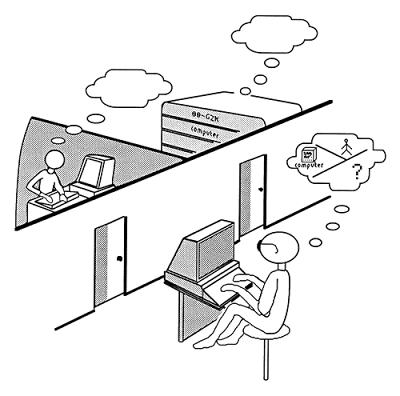
\includegraphics[width=0.6\textwidth]{img/teste-turing}
	\caption{Ideia geral do Teste de Turing}
	\label{fig:teste-turing}
\end{figure}

Logo, o Teste de Turing avalia se uma entidade é inteligente de acordo com a dimensão ``\textit{a entidade se comporta como um humano}''. O teste não avalia se a máquina pensa como um ser humano, pois não tem acesso à forma como a resposta foi inferida. Também não avalia a racionalidade, uma vez que:
\begin{itemize}
	\item O interrogado (seja o computador ou o humano) pode errar a resposta de alguma pergunta.
	\item Pode tomar uma decisão errada, ou não optar pela melhor decisão possível.
\end{itemize}

\insertspace

Até o momento, nenhuma máquina passou no teste, que ganhou popularidade por exigir uma série de capacidades da IA:
\begin{itemize}
	\item Processamento de linguagem natural
	\item Representação do conhecimento
	\item Raciocínio automatizado
	\item Aprendizagem de máquina
\end{itemize}
	
\insertspace
	
Considere as perguntas a seguir. Elas são simples de responder, mas não tão triviais a um computador.
\begin{itemize}
	\item Por que os cachorros não voam no inverno?
	\item O que você acha da papelaria de Presidente Getúlio?
\end{itemize}

\section{Hipóteses da IA}

Uma abordagem mais filosófica da IA sugere duas hipóteses: IA fraca e IA forte. A hipótese da IA fraca sugere que as máquinas podem \textbf{agir de maneira inteligente} (ou agir como se fossem inteligentes). A hipótese da IA forte sugere que as máquinas agem de forma inteligente porque \textbf{podem pensar} (quando o fazem, estão realmente pensando como um ser humano ou um ser racional).

\textbf{Em resumo:} simulação de inteligência (IA fraca) \textit{versus} inteligência real (IA forte).

\subsection{IA Fraca}
A IA fraca simula o pensamento ou comportamento inteligentes. Isto é, esta hipótese não se importa se a máquina está de fato pensando, ou se apenas segue um modelo que a leva para o resultado desejado. Esta hipótese preocupa-se em apresentar um comportamento inteligente. O Teste de Turing se preocupa em identificar entidades que são dotadas de inteligência seguindo esta abordagem. A pregunta que esta vertente busca responder é: \textit{as máquinas podem agir com inteligência}?

\subsection{IA Forte}

A IA forte visa o desenvolvimento de máquinas auto-conscientes. Ou seja, máquinas que efetivamente podem pensar. Esta abordagem considera ainda que a entidade, no seu processo cognitivo, é capaz de sentir, contêm emoções e são capazes de expressá-las. A pergunta que esta vertente busca responder é: \textit{as máquinas podem realmente pensar}? Como esperado, esta abordagem gera muitas discussões em torno da real possibilidade de se concretizar no futuro. Além disso, outros questionamentos se baseiam na ética em torno dos seus objetivos.

\section{Histórico}

A partir de 1943 alguns pesquisadores se dedicavam a estudar conceitos que se tornariam as bases para o que conhecemos hoje por inteligência artificial. Este período é chamado de \textit{gestação} da IA, que nasce no ano de 1956. A partir disso, foram anos de desenvolvimento acelerado da área e resultados otimistas. Mesmo assim, a área sofreu um período difícil pela dificuldade em tratar problemas reais, gerando perda de investimentos. Finalmente, a IA torna-se comercial principalmente pelos sistemas de apoio à tomada de decisão, bem como torna-se uma área de pesquisa científica, resultando no cenário atual. Abaixo apresenta-se um resumo da evolução da IA e dos seus principais marcos ao longo dos anos.

\insertspace

\begin{itemize}
	\item \textbf{1943:} modelagem de um neurônio artificial por Warren McCulloch e Walter Pitts e a ideia de simular o funcionamento do cérebro com uma rede de neurônios.
	
	\item \textbf{1950:} apresentação de uma visão completa da IA por Alan Turing, no seu artigo ``Computing Machinery and Intelligency''. Foram apresentados os conceitos de aprendizagem de máquina, algoritmos genéticos e aprendizagem por reforço.

	\item \textbf{1951:} primeira rede neural (SNARC), por Mrvin Minsky e Dean Edmonds.
	
	\item \textbf{1952:} aplicação de IA em jogos (damas, por exemplo), utilizando conceitos de aprendizagem de máquina, por Arthur Samuel.
	
	\item \textbf{1956:} considerado o nascimento da IA, por conta de um seminário organizado em Dartmouth College.
	\begin{itemize}
		\item Destaque para o programa de raciocínio \textit{Logic Theorist} (LT), criado por Allen Newell e Herbert Simon.
	\end{itemize}
	
	\item \textbf{1958:} John McCarthy cria a linguagem Lisp e, com ela, cria o primeiro sistema de IA completo: Advice Taker.
	\begin{itemize}
		\item Conceitos de representação do conhecimento e raciocínio.
	\end{itemize}
	
	\item \textbf{1960's:} rápida evolução das técnicas através da aplicação em problemas específicos, chamados \textit{minimundos}.
	\begin{itemize}
		\item Paralelo a isso, os pesquisadores perceberam que os métodos desenvolvidos eram limitados e resolver problemas da prática era um desafio ainda distante de ser alcançado.
		\item Exemplos: problemas com explosão combinatória; tradução de documentos.
	\end{itemize}
	
	\item \textbf{1970's:} incorporação de conhecimento do domínio para a resolução de problemas.
	\begin{itemize}
		\item Conceito de sistemas especialistas, que utilizam a representação do conhecimento e estratégias de raciocínio que exploram este conhecimento.
		\item Aplicações: DENDRAL, MYCIN.
	\end{itemize}
	
	\item \textbf{1980:} IA como uma indústria (aplicações comerciais).
	\begin{itemize}
		\item R1: primeiro sistema especialista comercial (1982).
		\item Grandes corporações investiam em um setor de IA, economizando milhões de dólares por ano.
	\end{itemize}
	
	\item \textbf{1987:} IA como uma ciência.
	\begin{itemize}
		\item Base nos fundamentos e teorias de outras áreas correlatas.
		\item Evolução dos métodos e bons resultados.
	\end{itemize}
	
	\item \textbf{1995:} conceito de agentes inteligentes.
	\begin{itemize}
		\item Formalização de uma estrutura para sistemas inteligentes.
		\item Um agente se divide em percepção, raciocínio e ação.
	\end{itemize}
	
	\item \textbf{1997:} Deep Blue versus Kasparov em uma disputa de xadrez.
	\begin{itemize}
		\item Kasparov: ``Senti uma nova espécia de inteligência do outro lado do tabuleiro.''
	\end{itemize}
	
	\item \textbf{2004:} agentes inteligentes na exploração espacial.
	
	\item \textbf{2007:} veículos autônomos.
	
	\item \textbf{2017:} uma máquina (AlphaGo) vence o melhor jogador de Go do mundo.
\end{itemize}


\section{Paradigmas}

Existem três paradigmas para a inteligência artificial: simbólico, conexionista e evolutivo. Estes paradigmas direcionam as pesquisas para a construção de sistemas inteligentes e apresentam técnicas sob diferentes perspectivas. A IA acabou dividindo-se em diferentes paradigmas por pesquisadores explorá-la através de diferentes caminhos: a IA deve se basear no estudo da psicologia (forma como entidades inteligentes raciocinam) ou da biologia (funcionamento estruturas biológicas que permitem o raciocínio)?

\subsection{IA simbólica}
Se baseia na representação do conhecimento através de símbolos. Este conhecimento é manipulado e, sobre ele, são realizadas inferências para a geração de novos conhecimentos. O exemplo mais comum de método simbólico na IA são os sistemas especialistas. As principais técnicas utilizadas são a lógica (proposicional e de primeira ordem) e a otimização.

\subsection{IA conexionista}
Se baseia na construção de sistemas inteligentes com base no funcionamento do cérebro humano, seus neurônios e conexões neurais. A inteligência do sistema emerge do funcionamento individual de cada neurônio, bem como da comunicação entre eles. Logo, este ramo é representado pelas redes neurais.

\subsection{IA evolutiva}
Este paradigma sugere que um sistema pode evoluir, de tal forma a tornar-se mais inteligente. Ou ainda, seus métodos propõem a evolução de soluções para problemas específicos. Esta evolução é obtida através de recombinações e mutações. O ramo mais conhecido deste paradigma são os algoritmos genéticos (bem como programação genética).

\section{Recursos disponíveis}

Existem softwares para uso pessoal que adotam técnicas de inteligência artificial no seu funcionamento interno. Exemplos são os assistentes pessoais que qualquer pessoa pode ter em seu smartphone ou computador. A Apple possui a Siri~\footnote{\url{https://support.apple.com/pt-br/HT204389}}, enquanto a Microsoft possui o Cortana~\footnote{\url{https://www.microsoft.com/pt-br/windows/cortana}} e a Google possui o Google Now~\footnote{\url{https://www.google.com/intl/pt-BR/landing/now/}}. Aplicações com inteligência artificial das mais diversas naturezas também estão disponíveis a usuários finais. Esta postagem~\footnote{\url{https://goo.gl/zXTnE8}} apresenta algumas delas.

Por outro lado, também existem diversas ferramentas para suporte a desenvolvedores que desejam construir aplicações com recursos de inteligência artificial. O PredictionIO~\footnote{\url{http://predictionio.incubator.apache.org}} é um servidor de aprendizagem de máquina para a criação de motores de predição. O Eclipse Deeplearning4j~\footnote{\url{https://projects.eclipse.org/proposals/eclipse-deeplearning4j}} é uma biblioteca de \textit{deep learning} para desenvolvedores Java com uma série de recursos disponíveis. A Microsoft apresenda o Azure~\footnote{\url{https://azure.microsoft.com/pt-br/overview/ai-platform/}}, que dentre uma série de outros recursos, possui uma plataforma de inteligência artificial com diversos serviços para desenvolvedores. Protégé~\footnote{\url{https://protege.stanford.edu}} é um framework para desenvolvimento de sistemas inteligentes baseados em conhecimento e que utilizem ontologias para sua representação. O Watson~\footnote{\url{https://www.ibm.com/watson/}} da IBM é uma plataforma que disponibiliza uma variedade de ferramentas de inteligência artificial, com exemplos de código e aplicações tanto para desenvolvedores como usuários finais. O DiffBlue~\footnote{\url{http://www.diffblue.com/}} é uma ferramenta para automação de código, que oferece serviços como localização de erros, refatoração de código e testes. O TensorFlow~\footnote{\url{https://www.tensorflow.org/}} da Google é uma plataforma para projetos de aprendizagem de máquina que disponibiliza uma variedade de recursos para desenvolvedores. O Nervana Neon~\footnote{\url{https://ai.intel.com/neon/}} é uma bilbioteca em Python para aprendizagem de máquina. Finalmente, o Neural Designer~\footnote{\url{https://www.neuraldesigner.com/}} é uma ferramenta que fornece suporte a tarefas de aprendizagem de máquina baseadas em redes neurais.

Ao longo dos capítulos seguintes, serão apresentados recursos específicos para os conteúdos estudados neste material, os quais poderão ser utilizados no desenvolvimento e solução dos exercícios propostos.

\section{Exercícios}

\begin{exercise}
Defina com suas próprias palavras: (a) inteligência, (b) inteligência artificial e (c) racionalidade.
\end{exercise}

\begin{exercise}
Suponha que a inteligência artificial seja utilizada para desenvolvimento de um sistema que atinja um grau 200 em um teste padrão de QI. Nesse caso, teríamos um programa mais inteligente que um ser humano? Explique.
\end{exercise}

\begin{exercise}
Até que ponto os sistemas seguintes são instâncias de inteligência artificial?
\begin{itemize}
	\item Leitores de código de barra de supermercados.
	\item Menus de voz de telefones.
	\item Mecanismos de busca na Web.
	\item Algoritmos de roteamento da Internet que respondem dinamicamente ao estado da rede.
\end{itemize}
\end{exercise}

\begin{exercise}
Todo ano o prêmio Loebner é entregue ao programa que chega mais perto de ser aprovado em uma versão do teste de Turing. Pesquise sobre o último vencedor do prêmio Loebner, comentando sobre os conceitos de inteligência artificial utilizados por ele.
\end{exercise}

\begin{exercise}
Examine a literatura de IA para descobrir se as tarefas a seguir podem ser resolvidas atualmente por computadores. Após isso, comente sobre as dificuldades das tarefas inviáveis.

\begin{enumerate}[a.]
	\item Jogar uma partida de tênis de mesa.
	\item Dirigir no centro do Cairo, Egito.
	\item Comprar mantimentos para uma semana no mercado.
	\item Comprar mantimentos para uma semana na Web.
	\item Jogar uma partida decente de \textit{bridge} em nível competitivo.
	\item Descobrir e provar novos teoremas matemáticos.
	\item Escrever uma história intencionalmente engraçada.
	\item Dar assessoria jurídica competente em uma área especializada de direito.
	\item Traduzir o inglês falado ao sueco falado, em tempo real.
	\item Executar uma operação cirúrgica complexa.
\end{enumerate}

\end{exercise}
\chapter{Agentes inteligentes}
\label{cap:agentes-inteligentes}

\framebox[\textwidth]{
	\hspace{1em}
	\vbox{
		\textbf{Leitura obrigatória:}
		\begin{itemize}
			\item \cite{RusselAndNorvig2010} -- Cap. 2 (Introdução).
		\end{itemize}
		
		\textbf{Leitura complementar:}
		\begin{itemize}
			\item \cite{Wooldridge2009} -- Cap. 2 (Intelligent Agents).
		\end{itemize}
	}
}

\section{Por que agentes?}

Muitos pesquisadores da área da inteligência artificial utilizam o conceito de agentes na construção de um sistema inteligente. Uma entidade computacional é, portanto, um agente que percebe seu ambiente e atua sobre ele em busca do seu objetivo. Dessa forma, podemos pensar em \textbf{agentes inteligentes} e \textbf{agentes racionais}, fazendo uso das ideias apresentadas no Capítulo~\ref{cap:introducao}. \citet{RusselAndNorvig2010} utilizam o conceito de agentes para definir um conjunto de princípios de projeto para a construção de sistemas inteligentes e norteiam o estudo da inteligência artificial em função destes conceitos. Logo, quando projetamos uma entidade dotada de inteligência artificial, estamos definindo um agente inteligente (ou agente racional).

\textbf{OBS:} existe uma vertente da inteligência artificial que estuda com maior profundidade os agentes inteligentes e os sistemas multiagente (sistema composto por um conjunto de agentes que interagem entre si). Para mais detalhes sobre este ramo, veja \citet{Weiss1999} e \citet{Wooldridge2009}.

\section{Conceitos básicos}

Esta seção apresenta os conceitos fundamentais de agentes inteligentes e ambientes, bem como sua relação com a construção de sistemas inteligentes.

\subsection{O que é um agente?}

\citet{RusselAndNorvig2010} definem agente como uma entidade (de software ou não) capaz de perceber seu \textbf{ambiente} por meio de \textbf{sensores} e atuar sobre o ambiente por meio de \textbf{atuadores}. Considerando ambiente como um provedor de entradas e receptor de saídas, podemos concluir que qualquer programa é um agente (tudo é um agente). Este conceito será utilizado no decorrer deste material, para a definição de agentes capazes de realizar tarefas com o uso de conceitos de inteligência artificial. No entanto, alguns autores questionam esta definição genérica de agentes, incluindo algumas características que diferem um simples programa computacional de um agente. \citet{FranklinAndGraesser1996} apresentam definições de vários autores e discutem sobre os pontos em comum e as diferenças nos conceitos fundamentais da área.

\textbf{Definição de \citet{FranklinAndGraesser1996}}
\begin{quotation}
``\textit{an \textbf{autonomous} agent is a system situated within and a part of an \textbf{environment} that \textbf{senses} that environment and \textbf{acts} on it, over time, in pursuit of its own \textbf{agenda} and so as to affect what it senses in the future}.''
\end{quotation}

\insertspace

\textbf{Definição de \citet{Wooldridge2009}}
\begin{quotation}
``\textit{a computer system that is situated in some \textbf{environment} and that is capable of independent (\textbf{autonomous}) \textbf{action} in this environment on behalf of its user or owner (figuring out what needs to be done to satisfy design \textbf{objectives}, rather than constantly being told)}.''
\end{quotation}

\insertspace

Algumas características gerais podem ser listadas a partir dessas definições:

\begin{itemize}
	\item O agente sempre está situado em um ambiente, percebe (sensores) seu estado e atua (atuadores) sobre ele.
	\item O agente deve ser autônomo, isto é, toma suas próprias decisões.
	\item O agente possui um objetivo, que conduz a sua tomada de decisões.
\end{itemize}

\insertspace

\begin{figure}[h]
	\centering
	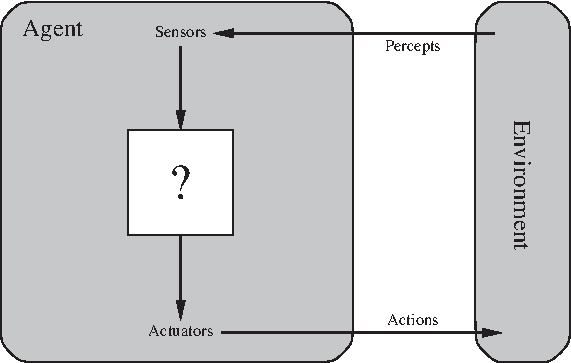
\includegraphics[width=0.5\textwidth]{img/agente-ambiente}
	\caption{Esquema geral de um agente e seu ambiente}
	\label{fig:agente-ambiente}
\end{figure}

A Figura~\ref{fig:agente-ambiente} apresenta o esquema geral de um agente e sua interação com o ambiente no qual está situado. O agente percebe o estado do seu ambiente através de sensores, infere sobre o que deve ser feito (tomada de decisão), e atua sobre o ambiente por meio de seus atuadores. A caixa representada por um sinal ``\textbf{?}'' define o funcionamento interno do agente. Ou seja, este elemento representa a implementação do agente, sua autonomia, seus objetivos e as técnicas de inteligência artificial utilizada por ele.

\subsection{Comportamento dos agentes}

Uma vez conhecido o conceito de agente, uma parte importante do seu projeto e implementação é a determinação do seu comportamento. Ou seja, como o agente processa as entradas, toma decisões e atua sobre o ambiente. A \textbf{percepção} é, portanto, aquilo que o agente enxerga do seu ambiente (seu estado). Um agente pode escolher uma ação não somente em função da sua percepção atual, mas da sequência de percepções obtidas anteriormente. A esta sequência de percepções damos o nome de história do agente.

Uma das formas de definirmos o comportamento do agente é através da construção de uma tabela que mapeia sequências de percepções para as ações desejadas. Este mapeamento é chamado de \textbf{função do agente} e sua implementação é chamada \textbf{programa do agente}. Na maioria dos casos, esta tabela seria infinita e, portanto, uma tabulação completa é impossível.

\textbf{Exemplo -- agente aspirador de pó:} o agente consiste em um robô cuja tarefa é aspirar o pó do chão. O ambiente é composto por dois quadrados (A e B). O agente percebe em qual quadrado está e se há sujeira, e pode (1) mover-se para a direita, (2) mover-se para a esquerda, (3) aspirar a sujeira ou (4) não fazer nada. A Figura~\ref{fig:agente-aspirador} ilustra o cenário apresentado.

\begin{figure}[h]
	\centering
	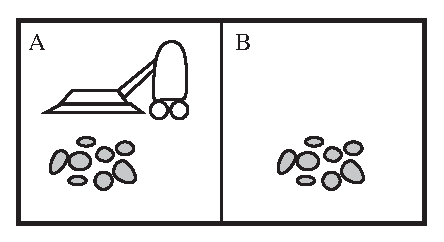
\includegraphics[width=0.5\textwidth]{img/agente-aspirador.eps}
	\caption{Agente aspirador e seu ambiente}
	\label{fig:agente-aspirador}
\end{figure}

A Tabela~\ref{tab:tabulacao-agente-aspirador} apresenta a função de agente do robô aspirador. Neste caso, a história completa do agente não é relevante. Basta ele perceber o estado do quadro em que se encontra (sujo ou limpo), para decidir sobre qual ação executar. No entanto, outras situações podem fazer uso do histórico para inferir sobre qual a melhor ação possível. Um ponto importante é: \textit{qual a melhor função de agente possível?} Ou seja, o que torna o agente bom ou ruim, inteligente ou não?

\begin{table}[h]
	\centering
	\begin{tabular}{p{13cm}l}
		\hline
		\textbf{Sequência de percepções} & \textbf{Ação} \\
		\hline
		$[$\textit{A}, \textit{Limpo}$]$ & \textit{Direita} \\
		$[$\textit{A}, \textit{Sujo}$]$ & \textit{Aspirar} \\
		$[$\textit{B}, \textit{Limpo}$]$ & \textit{Esquerda} \\
		$[$\textit{B}, \textit{Sujo}$]$ & \textit{Aspirar} \\
		$[$\textit{A}, \textit{Limpo}$]$, $[$\textit{A}, \textit{Limpo}$]$ & \textit{Direita} \\
		$[$\textit{A}, \textit{Limpo}$]$, $[$\textit{A}, \textit{Sujo}$]$ & \textit{Aspirar} \\
		$\vdots$ & $\vdots$ \\
		$[$\textit{A}, \textit{Limpo}$]$, $[$\textit{A}, \textit{Limpo}$]$, $[$\textit{A}, \textit{Limpo}$]$ & \textit{Direita} \\
		$[$\textit{A}, \textit{Limpo}$]$, $[$\textit{A}, \textit{Limpo}$]$, $[$\textit{A}, \textit{Sujo}$]$ & \textit{Aspirar} \\
		$\vdots$ & $\vdots$ \\
		\hline
	\end{tabular}
	\caption{Função de agente do robô aspirador}
	\label{tab:tabulacao-agente-aspirador}
\end{table}

Para definir o quão bom um agente é na realização de uma tarefa, precisamos de uma \textbf{medida de desempenho}, que determina o sucesso do comportamento de um agente, geralmente expresso quantitativamente. Em muitos casos chamaremos esta medida de \textbf{função objetivo}. Esta medida de desempenho deve ser imposta pelo projetista e, em geral, diz respeito ao estado do ambiente após a sequência de ações executadas pelo agente. Se o estado do ambiente é o estado desejado para a tarefa, o agente obteve sucesso. Nem sempre a definição da medida de sucesso é uma tarefa simples.

No exemplo do agente aspirador de pó, as seguintes medidas de sucesso poderiam ser definidas:
\begin{itemize}
	\item \textbf{\textit{Quantidade de sujeira limpa por dia}:} o agente pode repetir as ações de limpar a sujeira e jogá-la novamente no chão, maximizando sua medida de desempenho.
	\item \textbf{\textit{Quantidade de quadrados limpos no final do dia}:} o agente se limitaria a manter os dois quadrados limpos.
	\item \textbf{Conclusão:} é importante planejar a medida de desempenho em função da real expectativa de resultado.
	\item \textbf{Questões adicionais:} e se, além do chão limpo, quiséssemos minimizar o consumo de energia elétrica e a emissão de ruído?
\end{itemize}

\insertspace

Com base nestas informações, o conceito de \textbf{racionalidade} consiste em tomar a melhor decisão possível, levando em consideração os seguintes aspectos:
\begin{itemize}
	\item A medida de desempenho (critério de sucesso)
	\item O conhecimento do agente sobre o ambiente
	\item As ações que o agente pode executar
	\item A sequência de percepções do agente até o momento
\end{itemize}

\insertspace

Um \textbf{agente racional} é, portanto, um agente que toma suas decisões com racionalidade. Ou seja, um agente racional toma a melhor decisão que pode, conforme sua medida de desempenho, seu conhecimento, suas ações e percepções. \citet{RusselAndNorvig2010} apresentam uma definição formal para um agente racional:

\begin{quotation}
	\textit{``Para cada sequência de percepções possível, um agente racional deve selecionar uma ação que se espera venha a maximizar sua medida de desempenho, dada a evidência fornecida pela sequência de percepções e por qualquer conhecimento interno do agente.''}
\end{quotation}

Considere um agente aspirador de pó que limpa um quadrado se ele estiver sujo e passa para o outro quadrado se o primeiro não estiver sujo (repetidamente executa esta sequência de ações). Para definir se o mesmo é ou não racional, é necessário analisar o contexto no qual o agente se encontra segundo os fatores envolvidos no conceito de racionalidade (apresentados acima).
\begin{itemize}
	\item \textbf{Medida de desempenho:} o agente recebe um ponto para cada quadrado limpo ao fim do dia, ao longo de uma duração de 1000 dias;
	\item \textbf{Conhecimento do agente sobre o ambiente:} o agente conhece a ``geografia'' do ambiente e desconhece sua posição inicial e a distribuição da sujeira. Quadrados limpos permanecem limpos até o fim do dia. A ação de aspiração limpa o quadrado atual. As ações \textit{esquerda} e \textit{direita} movem o agente para o quadrado ao lado (conforme lado escolhido). O agente não pode movimentar-se para fora do ambiente.
	\item \textbf{As ações disponíveis:} \textit{esquerda}, \textit{direita}, \textit{aspirar} e \textit{nada} (não fazer nada).
	\item \textbf{Sequência de percepções:} o agente percebe sua posição e se a posição contém sujeira.
\end{itemize}

Podemos concluir que o agente em questão é racional, pois obterá a máxima pontuação possível (medida de desempenho) executando o comportamento apresentado. No entanto, se adicionarmos novas circunstâncias ao cenário, este mesmo agente pode passar a ser irracional. Se a medida de desempenho incluir o consumo de energia, existem funções de agente melhores (que não oscilam entre os quadrados após estarem limpos).

\subsection{Conceitos adicionais}

É importante destacar a diferença entre um agente racional e um agente onisciente (\textbf{racionalidade não é onisciência}). Um agente racional escolhe ações que maximizam a sua recompensa (maximiza a sua medida de desempenho). No entanto, em ambientes reais (ou suficientemente complexos) existem fatores externos ao conhecimento e percepções do agente, que podem afetar o resultado de uma ação. Por exemplo, o agente aspirador de pó pode selecionar a ação aspirar sem saber que junto da sujeira encontra-se uma substância danosa ao seu funcionamento. Neste caso, uma vez que o chão contém sujeira e o agente não sabe da substância danosa, a ação racional é aspirar a sujeira. Esta ação, mesmo que racional, leva a um resultado muito ruim.

Por outro lado, um agente onisciente possui conhecimento completo do contexto no qual está inserido. Ele decide sobre suas ações considerando todas as variáveis que podem influenciar no resultado final (em um valor menor ou maior de medida de desempenho). Em resumo, um agente racional maximiza o \textit{retorno esperado} de suas ações, enquanto um agente onisciente maximiza o \textit{retorno real} de suas ações.

Como na maior parte das vezes um agente racional não conhece completamente seu ambiente, uma estratégia racional é tomar ações que o permitam coletar informações. Por exemplo, o agente aspirador de pó poderia, antes de selecionar a ação \textit{aspirar}, executar a ação \textit{verificar}, que checa se existe alguma substância danosa na sujeira. Ou ainda, se modificarmos o ambiente deste agente para um conjunto de quadrados desconhecidos, o agente deveria executar ações de \textbf{exploração} do ambiente.

Paralelo às habilidades de coleta de informações e de exploração, um agente deve ser capaz de \textbf{aprender} ao longo do tempo. Em geral, o agente já possui um conhecimento prévio do ambiente, definido pelo projetista. Se este conhecimento for parcial e/ou limitado, ou ainda se o ambiente muda com o passar do tempo, um agente sem capacidade de adquirir novos conhecimentos dificilmente resolverá a tarefa com qualidade. Aprender significa utilizar a experiência para atualizar seu comportamento.

Quando um agente se comporta com base estritamente no conhecimento definido pelo projetista, este agente não possui \textbf{autonomia}. A medida que o agente aprende e passa a se comportar com base no conhecimento adquirido, dizemos que o agente é autônomo. Neste sentido, o agente inicialmente possui pouco conhecimento e a habilidade de aprender. Com o passar do tempo, o agente, autônomo e racional, pode se tornar independente do seu conhecimento prévio.

\section{O ambiente dos agentes}

Esta seção define o ambiente dos agentes e apresenta algumas propriedades destes ambientes, que o tornam mais ou menos complexos e impactam no projeto e implementação de agentes.

\subsection{Ambiente de tarefa}

O primeiro passo no projeto de um agente inteligente é a definição do seu \textbf{ambiente de tarefa}, composto pela medida de desempenho, ambiente, atuadores (ações) e sensores (percepções) do agente. Apesar do simples exemplo do aspirador de pó, a maioria dos ambientes são complexos e possuem características que dificultam a tarefa a ser executada (o que torna desafiador o campo de estudo da inteligência artificial). A Tabela~\ref{tab:ambientes-tarefa} apresenta alguns exemplos de ambientes de tarefa com diferentes níveis de complexidade.

\begin{table}[h]
	\centering
	\small
	\rowcolors{2}{white}{gray!25}
	\begin{tabular}{L{2cm} L{3cm} L{3cm} L{2.9cm} L{2.9cm}}
		\hline
		\rowcolor{black}
		\color{white}\textbf{Agente} & \color{white}\textbf{Medida de desempenho} & \color{white}\textbf{Ambiente} & \color{white}\textbf{Atuadores} & \color{white}\textbf{Sensores} \\
		\hline
		Veículo autônomo & Viagem segura, rápida, dentro da lei, minimizando tempo e consumo & Estradas, tráfego, pedestres, sinalização & Pedais, direção, sinal, buzina & Câmeras, sonar, velocímetro, GPS, hodômetro e acelerômetro  \\
		Sistema de diagnóstico médico & Acerto da doença, minimizar custos & Paciente, hospital, equipe & Painel de exibição de perguntas, testes, diagnósticos, tratamentos e indicações & Teclado para informar os sintomas \\
		Sistema de análise de imagens de satélite & Classificação correta da imagem & Link de transmissão & Monitor para exibir a categorização da imagem & Leitor de array de pixels \\
		Robô de seleção de peças & Percentual de peças na bandeja correta & Correia transportadora com peças, bandejas & Braço e mão articulados & Câmera, sensores angulares articulados \\
		Instrutor de inglês interativo & Maximizar nota do aluno em teste & Alunos, testes de agência & Monitor para exibir exercícios, sugestões e correções & Teclado para entrada de informações \\
		\hline
	\end{tabular}
	
	\caption{Exemplos de ambientes de tarefa}
	\label{tab:ambientes-tarefa}
\end{table}

Observações:
\begin{itemize}
	\item Alguns agentes são projetados para trabalhar em ambientes físicos (ex: veículo autônomo), enquanto outros se limitam a ambientes virtuais (ex: sistema de análise de imagens). Os agentes que operam exclusivamente em ambientes virtuais são chamados de \textbf{agentes de software}.
	
	\item Existem ambientes de tarefa (consequentemente os próprios agentes) simples e complexos, tanto em ambiente físico quanto virtual.
	\begin{itemize}
		\item \textbf{Agentes físicos:} aspirador de pó (simples) e robô para cuidado de pessoas idosas (complexo).
		\item \textbf{Agentes de software:} sistema para análise de palavras ofensivas em postagens (simples) e softbot para monitoramento do mercado financeiro (complexo).
	\end{itemize}
	
	\item A robótica é um importante (e vasto) campo de estudos no projeto e desenvolvimento de agentes físicos.
	
	\item Esta disciplina foca no estudo de agentes de software.
\end{itemize}

\subsection{Propriedades dos ambientes}

Os ambientes de tarefa podem ser classificados segundo seis dimensões. Estas dimensões balizam o projeto de agentes e a escolha da técnica de IA adequada para ele. Esta seção mostra a definição destas dimensões, as classificações existentes e alguns exemplos. Podemos adiantar que o caso mais difícil é um ambiente parcialmente observável, estocástico, sequencial, dinâmico, contínuo e multiagente (tenha isso em mente ao estudar as diferentes propriedades de cada dimensão). A tarefa de veículo autônomo, por exemplo, possui este nível de dificuldade.

\subsubsection{1. Completamente observável $\times$ parcialmente observável}

\begin{itemize}
	\item Se o agente consegue acessar o estado completo (ou pelo menos todas as informações que lhe importa) do ambiente, ele é completamente observável e, caso contrário, ele é parcialmente observável.
	
	\item Um ambiente pode ainda ser parcialmente observável quando as entradas são sensíveis a ruídos ou quando os sensores são imprecisos.
	
	\item \textbf{Aspirador de pó completamente observável:} o agente consegue observar todo o ambiente (dois quadrados).
	\item \textbf{Aspirador de pó parcialmente observável:} o agente possui um único sensor que só consegue verificar o quadrado atual.
\end{itemize}

\subsubsection{2. Determinístico $\times$ estocástico}

\begin{itemize}
	\item Se o próximo estado do ambiente é determinado pelo estado atual, mais a ação do agente, então o ambiente é determinístico. Se existem fatores externos que podem influenciar no próximo estado do ambiente, então ele é estocástico.
	
	\item Se o ambiente é determinístico exceto pelas ações de outros agentes, então ele é \textbf{estratégico}.
	
	\item \textbf{Aspirador de pó determinístico:} ele aspira a sujeira e o quadrado é limpo, os demais elementos do cenário permanecem no mesmo estado
	\item \textbf{Aspirador de pó estocástico:} o mecanismo de sucção não é confiável ou sujeira aparece aleatoriamente onde já estava limpo.
\end{itemize}

\subsubsection{3. Episódico $\times$ sequencial}

\begin{itemize}
	\item No caso episódico, a experiência do agente é dividida em episódios atômicos (iterações), onde o agente percebe o ambiente e executa uma ação. A escolha da ação do episódio não depende de episódios anteriores. No caso sequencial, uma ação pode modificar a escolha de ações futuras.
	
	\item Ambientes episódicos são mais simples, pois o agente não precisa pensar à frente. A classificação de uma peça não afeta a classificação das demais peças. Porém, uma jogada de xadrez pode afetar as demais jogadas e, por isso, o agente deve pensar nas consequências da ação no futuro.
	
	\item \textbf{Aspirador de pó episódico:} se o aspirador tivesse apenas a função de classificar um quadrado como sujo ou limpo.
	\item \textbf{Aspirador de pó sequencial:} considerando que a sujeira não retorna, a ação de limpar um quadrado implica no robô não precisar voltar ao referido quadrado no futuro.
\end{itemize}

\subsubsection{4. Estático $\times$ dinâmico}

\begin{itemize}
	\item O ambiente é dito estático quando ele não se altera com o passar do tempo. Isto é, desde que o agente percebe o ambiente até o momento da deliberação de uma ação, o ambiente possui o mesmo estado. Por outro lado, se o ambiente muda de estado enquanto o agente delibera, ele é dito dinâmico.
	
	\item Em ambientes dinâmicos o agente deve continuar observando o ambiente até decidir sobre uma ação, o que o torna mais complexo.
	
	\item Se o ambiente não muda ao longo do tempo, mas sim o nível de desempenho do agente, o ambiente é dito \textbf{semidinâmico}. Por exemplo, um jogo de xadrez com tempo se encaixa nesta classificação.
	
	\item \textbf{Aspirador de pó estático:} uma vez verificado o estado (limpo ou sujo), o ambiente não se altera.
	\item \textbf{Aspirador de pó dinâmico:} o agente pode perceber um quadrado limpo e, antes de tomar uma decisão, uma nova sujeira aparece no ambiente.
\end{itemize}

\subsubsection{5. Discreto $\times$ contínuo}

\begin{itemize}
	\item Este conceito se aplica a: (1) estado do ambiente, (2) modo como o tempo é tratado, ou ainda (3) percepções do agente. Ou seja, se o ambiente possui um número finito de estados discretos ou se ele é medido de forma contínua; se o tempo é discreto ou contínuo; se o agente percebe seu ambiente de forma discreta ou contínua.
	
	\item \textbf{Aspirador de pó discreto:} os estados são discretos (quadrado sujo ou quadrado limpo).
	\item \textbf{Aspirador de pó contínuo:} o agente poderia perceber a quantidade de sujeira, que poderia ser medida de forma contínua.
\end{itemize}

\subsubsection{Agente único $\times$ multiagente}

\begin{itemize}
	\item Quando o ambiente de tarefa envolve apenas um agente, o ambiente é dito de agente único, ou ainda \textbf{monoagente}. Quando diferentes agentes estão envolvidos no ambiente, temos um cenário multiagente.
	
	\item Um ambiente multiagente pode ser ainda \textbf{colaborativo}, quando o sucesso de um agente leva ao sucesso do outro agente, ou \textbf{competitivo}, quando o sucesso de um agente leva ao insucesso do outro agente.
	
	\item \textbf{Aspirador de pó de agente único:} um único aspirador de pó responsável pela limpeza do ambiente.
	\item \textbf{Aspirador de pó multiagente colaborativo:} dois ou mais aspiradores de pó responsáveis pela limpeza do ambiente, onde a medida de desempenho do agente é a área total limpa.
	\item \textbf{Aspirador de pó multiagente competitivo:} dois ou mais aspiradores de pó responsáveis pela limpeza do ambiente, onde a medida de desempenho do agente é a quantidade de sujeira limpa por ele.
\end{itemize}

\section{Projeto de agentes}

Um agente é composto por uma \textbf{arquitetura} e um \textbf{programa}. A arquitetura define o ``corpo'' do agente, ou seja, qual a estrutura do agente em termos de sensores e atuadores. Nesta disciplina, consideramos que os agentes são softwares e, portanto, não nos preocuparemos com estruturas físicas. O programa de agente define a forma como o mesmo se comporta para a realização de suas tarefas. Em geral, dividimos os agentes em quatro tipos básicos: \textit{agentes reativos simples}, \textit{agentes reativos baseados em modelo}, \textit{agentes baseados em objetivos} e \textit{agentes baseados na utilidade}.

\subsection{Agentes reativos simples}

Os agentes reativos simples compõem o tipo mais simples de agente. Eles selecionam suas ações com base na percepção atual do estado do ambiente. Em outras palavras, \textit{o agente reage ao ambiente que percebe}. Para selecionar uma ação, estes agentes são definidos por regras na estrutura de \textbf{condição-ação}:

\begin{center}
	\textbf{se} \textit{condição} \textbf{então} \textit{ação}.
\end{center}

Por exemplo:

\begin{center}
	\textbf{se} \textit{chão está sujo} \textbf{então} \textit{aspirar}.
\end{center}

\insertspace

A Figura~\ref{fig:agente-reativo-simples} apresenta o esquema geral de um agente reativo simples. Em um primeiro momento o estado do mundo é percebido e interpretado. O conjunto de regras que o agente possui é utilizado para a tomada de decisão da próxima ação a ser executada. O comando da ação selecionada é então enviada aos atuadores.

\insertspace

\begin{figure}[h]
	\centering
	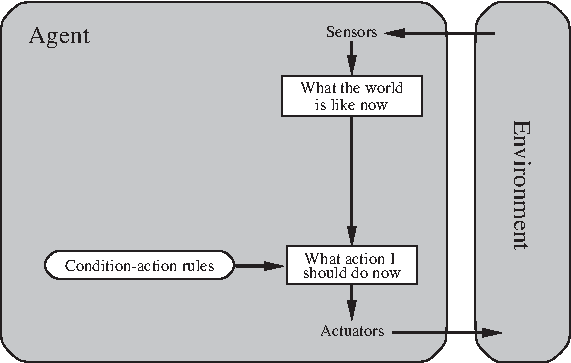
\includegraphics[width=0.5\textwidth]{img/agente-reativo-simples}
	\caption{Esquema geral de um agente reativo simples}
	\label{fig:agente-reativo-simples}
\end{figure}

O Algoritmo~\ref{alg:agente-reativo-simples} apresenta uma implementação básica para um agente reativo simples. A percepção é recebida através dos sensores do agente e é dada como entrada do algoritmo. A partir da percepção, é extraído o estado do ambiente (linha 2), que por sua vez serve de parâmetro para a seleção da regra correspondente (linha 3). Em geral, estes agentes selecionam a primeira regra cujas condições correspondem ao estado recuperado. A partir da regra selecionada, o agente extrai a ação a ser executada (linha 4), a qual é retornada e enviada aos atuadores.

\begin{algorithm}[h]
	\DontPrintSemicolon
	\Entrada{\textit{percepção}}
	\Saida{\textit{ação}}
	
	\Inicio{
		\textit{estado} $\gets$ INTERPRETAR-ENTRADA(\textit{percepção})\;
		\textit{regra} $\gets$ REGRA-CORRESPONDENTE(\textit{estado}, \textit{regras})\;
		\textit{ação} $\gets$ AÇÃO-DA-REGRA[\textit{regra}]\;
		\Retorna{\textit{ação}}
	}
	
	\caption{Pseudocódigo para um agente reativo simples}
	\label{alg:agente-reativo-simples}
\end{algorithm}

Podemos definir um agente reativo simples para o mundo do aspirador de pó. Dada sua simplicidade, o código deste agente pode ser ainda mais simples, uma vez que existem poucas regras. O Algoritmo~\ref{alg:agente-reativo-simples-aspirador} apresenta uma proposta de agente aspirador de pó reativo simples. Sempre que o estado da posição atual for \textit{Sujo}, o agente seleciona a ação \textit{Aspirar}. Caso contrário, ele move para o quadrado ao lado.

\begin{algorithm}[h]
	\DontPrintSemicolon
	\Entrada{\textit{percepção} na estrutura $[$\textit{posição},\,\textit{estado}$]$}
	\Saida{\textit{ação}}
	
	\Inicio{
		\Se{estado = Sujo}{
			\Retorna{\textit{Aspirar}}\;
		}\Senao{
			\Se{posição = A}{
				\Retorna{\textit{Direita}}\;
			}\Senao{
				\Retorna{\textit{Esquerda}}\;
			}
		}
	}
	
	\caption{Pseudocódigo para um agente aspirador de pó reativo simples}
	\label{alg:agente-reativo-simples-aspirador}
\end{algorithm}

Suponhamos que o sensor que determina a posição do robô estrague, levando-o a uma observação parcial do ambiente. Neste caso, o robô é capaz de apenas determinar se a posição em que se encontra está ou não com sujeira. Quando a posição estiver limpa, ele não consegue determinar para qual lado deve movimentar-se. Uma estratégia para superar esta dificuldade é fazer uso de \textbf{aleatoriedade} no momento de selecionar uma das ações de movimento. Ou seja, ele pode selecionar \textit{Direita} ou \textit{Esquerda} com probabilidade $0.5$. Em geral, agentes reativos simples possuem limitações, dada sua simplicidade, o que exige a adoção de técnicas como esta.


\subsection{Agentes reativos baseados em modelo}

Estes agentes são também chamados de \textbf{agentes deliberativos}. A ideia por trás dos agentes baseados em modelo consiste no agente ter uma representação do mundo (ambiente), de tal forma que ele entenda como o mundo funciona e como evolui com o passar do tempo. Um \textbf{modelo} é, portanto, a representação deste conhecimento que o agente possui do seu ambiente. Este modelo é construído e atualizado em função da sequência de percepções do agente. Neste sentido, o modelo é capaz de minimizar o problema da observação parcial do ambiente. Ou seja, caso o agente não consiga observar algum aspecto do ambiente, o modelo é capaz de determiná-lo (com certo nível de precisão).

A Figura~\ref{fig:agente-reativo-baseado-modelo} apresenta o esquema geral de um agente reativo baseado em modelo. Por ser um agente reativo, suas ações continuam sendo modeladas por regras condição-ação. No entanto, o agente mantém seu modelo do mundo (``como o mundo evolui'') que, juntamente com suas entradas sensoriais e as consequências de suas ações, serve para atualizar o estado percebido antes da tomada de decisão. Isto é, o estado é determinado pelas suas percepções do ambiente, seu conhecimento sobre aquilo que não foi possível perceber e as consequências da ação escolhida. Perceba que, para isso, o agente mantém uma representação interna do estado do ambiente.

\begin{figure}[h]
	\centering
	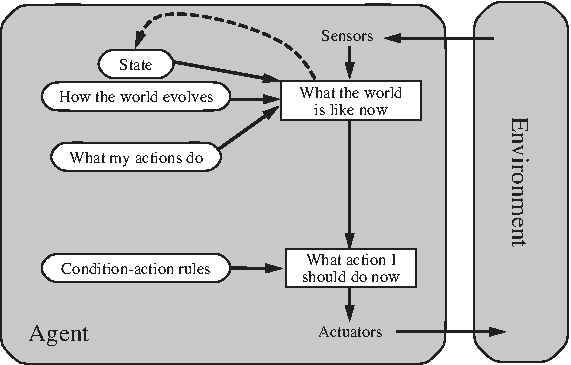
\includegraphics[width=0.5\textwidth]{img/agente-reativo-baseado-modelo}
	\caption{Esquema geral de um agente reativo baseado em modelo}
	\label{fig:agente-reativo-baseado-modelo}
\end{figure}

O Algoritmo~\ref{alg:agente-reativo-baseado-modelo} apresenta uma implementação básica para um agente reativo baseado em modelo. Em comparação com o pseudocódigo do agente reativo simples, a função \texttt{INTERPRETAR-ENTRADA} é substituída pela ação \texttt{ATUALIZAR-ESTADO} (linha 2). Antes, o agente só considerava suas percepções para definir o estado do ambiente. Agora, a percepção é utilizada em conjunto com o modelo e as ações do agente para determinar o estado do ambiente.

\begin{algorithm}[h]
	\DontPrintSemicolon
	\Entrada{\textit{percepção}}
	\Saida{\textit{ação}}
	
	\Inicio{
		\textit{estado} $\gets$ ATUALIZAR-ESTADO(\textit{estado}, \textit{ação}, \textit{percepção})\;
		\textit{regra} $\gets$ REGRA-CORRESPONDENTE(\textit{estado}, \textit{regras})\;
		\textit{ação} $\gets$ AÇÃO-DA-REGRA[\textit{regra}]\;
		\Retorna{\textit{ação}}
	}
	
	\caption{Pseudocódigo para um agente reativo baseado em modelo}
	\label{alg:agente-reativo-baseado-modelo}
\end{algorithm}

\subsection{Agentes baseados em objetivos}

Em muitos casos, não é suficiente manter uma representação do mundo e um conjunto de regras condição-ação. O agente pode deparar-se com situações de tomada de decisão em que é difícil definir a ação adequada. Neste caso, o agente deve manter um ou um conjunto de objetivos que descreva situações desejáveis. Por exemplo, um veículo autônomo que encontra um acidente de trânsito e precisa desviar seu caminho, escolhendo entre duas opções. Neste caso, seu objetivo é chegar no destino de sua viagem e a análise sobre qual rota tomar deve ser feita em função deste objetivo. Perceba que esta decisão não é tão simples como aquelas oriundas das regras condição-ação. Esta decisão deve considerar ações no futuro, definindo qual rota levará o agente a cumprir seu objetivo.

Os agentes baseados em objetivos são mais flexíveis, uma vez que o conhecimento que baliza suas decisões é representado explicitamente e pode ser facilmente modificado. Por exemplo, se começar a chover, o veículo autônomo tem o conhecimento de que o funcionamento do freio é alterado, bem como outros aspectos da dirigibilidade. Com isso, o veículo automaticamente ajusta todo o seu comportamento em função das novas condições climáticas. Para fazermos o mesmo com um agente reativo, teríamos que escrever um grande conjunto de regras condição-ação, que incluam a chuva como condição das novas ações.

\begin{figure}[h]
	\centering
	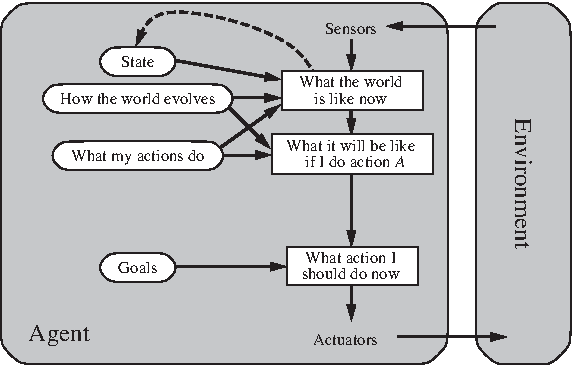
\includegraphics[width=0.5\textwidth]{img/agente-baseado-objetivos}
	\caption{Esquema geral de um agente baseado em objetivos}
	\label{fig:agente-baseado-objetivos}
\end{figure}

A Figura~\ref{fig:agente-baseado-objetivos} apresenta o esquema geral de um agente baseado em objetivos. Além de manter um estado interno, o modelo do seu ambiente e as consequências de suas ações, o agente mantém um conjunto de objetivos. Estes objetivos são utilizados na tomada de decisões, no lugar das regras condição-ação.

\subsection{Agentes baseados na utilidade}

Em geral, agentes baseados em objetivos utilizam seu conhecimento na tomada de decisões que atinjam seus objetivos. No entanto, esta abordagem não é suficiente para o desenvolvimento de agentes com alta qualidade. No exemplo do veículo autônomo, o agente escolherá pela rota que leve-o ao seu objetivo de chegar no destino da viagem. Se ambas as rotas o permitem chegar no seu destino, ele escolhe por qualquer uma das duas. Ou seja, seus objetivos servem para classificar as opções em alternativas de \textit{sucesso} e de \textit{insucesso}, na satisfação dos seus objetivos. Porém, se uma das rotas demora 5 minutos, enquanto a outra demora 30 minutos, é razoável optar pela primeira. Este comportamento não é obtido em um agente simples baseado em objetivos.

Para modelar este comportamento, definimos a \textbf{utilidade} como uma medida de recompensa na tomada de uma decisão. Neste sentido, a \textbf{função de utilidade} mapeia um estado (ou uma sequência de estados) em um número real que descreve o grau de sucesso (ou de felicidade) associado. Além de auxiliar na escolha de duas opções que levam ao objetivo, mas com graus de sucesso diferentes, a função de utilidade permite agir com inteligência em dois casos: (1) quando existem objetivos contraditórios e (2) quando incerteza no atingimento dos objetivos.
\begin{enumerate}[(1)]
	\item Considerando que o agente considera dois aspectos na escolha de rotas: tempo de viagem e desgaste do veículo. Se a primeira rota tem menor tempo e maior desgaste que a segunda, o agente terá que optar por um dos aspectos em detrimento do outro. A função de utilidade permite definir escolhas dessa natureza, onde o agente tem um compromisso com cada aspecto.
	\item Considerando que em ambas as rotas, não é certo que elas levam ao destino da viagem. Neste caso, a função de utilidade serve para definir a probabilidade de que cada rota leve ao destino, permitindo optar pela rota com maior valor de probabilidade.
\end{enumerate}

\begin{figure}[h]
	\centering
	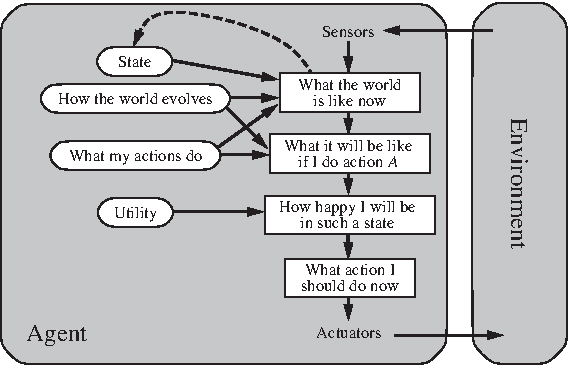
\includegraphics[width=0.5\textwidth]{img/agente-baseado-utilidade}
	\caption{Esquema geral de um agente baseado em utilidade}
	\label{fig:agente-baseado-utilidade}
\end{figure}

A Figura~\ref{fig:agente-baseado-utilidade} apresenta o esquema geral de um agente baseado em utilidade. Perceba que foram mantidos os componentes de um agente baseado em objetivos e que utiliza um modelo do mundo para tratar a observação parcial do ambiente. Agora, a tomada de decisão utiliza o conceito de utilidade para definir ``\textit{o quanto serei feliz em tal estado}'', optando pela ação que leva ao maior grau de felicidade. Em geral, agentes racionais utilizam esta estrutura interna, pois a racionalidade consiste em optar pela ação que maximiza os ganhos do agente, em termos de utilidade.

\subsection{Agentes com aprendizagem}

As seções anteriores apresentaram agentes com diferentes componentes, que definem a forma como eles se comportam. Em outras palavras, estes componentes definem a forma como as percepções são tratadas para a seleção de uma ação. Em agentes que aprendem com a experiência, são incluídos elementos que permitem ajustar os componentes citados, de tal forma que o comportamento seja aprimorado. A Figura~\ref{fig:agente-aprendizagem} mostra o esquema geral de um agente com aprendizagem, constituído por quatro componentes principais: \textit{elemento de desempenho}, \textit{elemento de aprendizado}, \textit{crítico} e \textit{gerador de problemas}.

\begin{figure}[h]
	\centering
	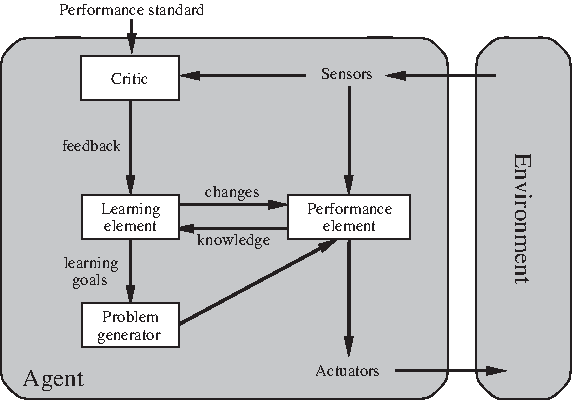
\includegraphics[width=0.5\textwidth]{img/agente-aprendizagem}
	\caption{Esquema geral de um agente com aprendizagem}
	\label{fig:agente-aprendizagem}
\end{figure}

O \textbf{elemento de desempenho} consiste na estrutura de tomada de decisão do agente, que recebe as percepções e delibera ações. Ou seja, este elemento contém uma das estruturas de componentes apresentadas nas seções anteriores (estrutura reativa simples, baseada em modelo, baseada em objetivos ou baseada na utilidade).

O \textbf{elemento de aprendizado} é responsável por ajustar o comportamento do agente, melhorando-o com o passar do tempo. Este elemento está em constante comunicação com o elemento de desempenho, pois sua tarefa é modificá-lo e receber o conhecimento obtido com a experiência. Por exemplo, o elemento de aprendizado cria novas regras e modifica as existentes no elemento de desempenho (considerando um agente reativo).

O \textbf{crítico} é responsável por medir o sucesso do agente sob o ponto de vista externo. Quando o agente executa uma determinada ação, o crítico informa o agente sobre o sucesso dela, de tal forma que o agente possa ajustar seu comportamento. Por exemplo, se o veículo autônomo fizer uma troca de pista brusca, ele atingiu seu objetivo interno de trocar de pista. No entanto, o ambiente externo (outros motoristas) mostra que não foi uma manobra segura. Esta consequência não é captada pelas percepções do agente e, portanto, é papel do crítico informar o elemento de aprendizado que esta manobra não deve ser realizada dessa forma. O elemento de aprendizado, por sua vez, inclui uma nova regra no elemento de desempenho, evitando situações similares no futuro. Ou seja, o agente aprendeu a não mudar de pista de forma brusca.

O \textbf{gerador de problemas} é responsável pelo comportamento exploratório do agente. Como vimos nas seções anteriores, o agente sempre seleciona a ação que lhe traz o maior retorno. Por exemplo, se uma rota leva ao destino e, no caso de uma segunda rota, não há certeza disso, o agente sempre seleciona a primeira rota. No entanto, se o agente explorar a segunda rota, pode descobrir um caminho mais curto para seu destino, ou descobrir que não é uma boa opção. Neste sentido, o gerador de problemas tem a tarefa de gerar situações de exploração, de tal forma que o agente aprenda com novas experiências.

\section{Recursos disponíveis}

Apesar de não ser necessário o uso de nenhuma tecnologia específica para o desenvolvimento de agentes, existem ferramentas que facilitam esta tarefa e fornecem uma arquitetura para a construção de agentes inteligentes. O Jason~\footnote{\url{http://jason.sourceforge.net/wp}} é uma extensão da linguagem AgentSpeak para o desenvolvimento de agentes e sistemas multiagentes. Outra linguagem bastante conhecida para o desenvolvimento de agentes em Java é o JADE~\footnote{\url{http://jade.tilab.com}}. O JaCaMo~\footnote{\url{http://jacamo.sourceforge.net}}, por sua vez, é um framework que combina a linguagem Jason com as tecnologias Cartago, para tratamento de artefatos, e Moise, para organizações de agentes.

Uma aplicação comum de sistemas multiagentes é a simulação de fenômenos do mundo real, área conhecida por simulação baseada em agentes. \cite{AbarEtAl2017} apresentam uma revisão atualizada dos softwares existentes para modelagem e simulação baseada em agentes. Uma ferramenta de destaque é o NetLogo~\footnote{\url{https://ccl.northwestern.edu/netlogo}}, que fornece um ambiente para o desenvolvimento de simulações baseadas em agentes de propósito geral. A linguagem fornece uma série de funções que facilitam o processo de desenvolvimento de sistemas dessa natureza.

\section{Exercícios}

\resetexercisenumbering

\begin{exercise}
Para cada uma das atividades (agente) abaixo, forneça uma descrição do ambiente de tarefa (medida de desempenho, ambiente, atuadores e sensores):
\begin{enumerate}[a.]
	\item Jogar futebol.
	\item Compra de livros usados de IA na Internet.
	\item Jogar uma partida de tênis.
	\item Praticar tênis contra uma parede.
	\item Realizar um salto em altura.
	\item Licitações de um item em um leilão.
\end{enumerate}
\end{exercise}

\begin{exercise}
Classifique os ambientes a seguir em: completamente observável ou parcialmente observável, determinístico ou estocástico (ou ainda, estratégico), episódico ou sequencial, estático ou dinâmico (ou ainda, semi-dinâmico), discreto ou contínuo, monoagente ou multiagente.

\begin{enumerate}[a.]
	\item Jogo de palavras cruzadas.
	\item Xadrez com relógio.
	\item Pôquer.
	\item Gamão.
	\item Veículo autônomo.
	\item Diagnóstico médico.
	\item Análise de imagens.
	\item Robô de seleção de peças.
	\item Controlador de refinaria.
	\item Instrutor interativo de inglês.
\end{enumerate}
\end{exercise}

\begin{exercise}
Implemente um simulador para o ambiente do aspirador de pó. Sua implementação deve ser modular, de forma que os sensores, atuadores e as características do ambiente (tamanho, forma, localização da sujeira, etc.) possam ser alterados facilmente.
\end{exercise}

\begin{exercise}
Implemente um agente reativo simples para o ambiente do aspirador de pó, usando o simulador desenvolvido no exercício anterior. Execute as simulações com diferentes posições de sujeira e de início do agente. Registre a pontuação de desempenho do agente para cada configuração e sua pontuação média global.
\end{exercise}

\begin{exercise}
Considere uma versão modificada do ambiente de aspirador de pó, na qual o agente é penalizado com um ponto para cada movimento.
\begin{enumerate}[a.]
	\item Um agente reativo simples pode ser perfeitamente racional para esse ambiente? Explique.
	\item E um agente reativo com estado? Projete tal agente.
	\item Como suas respostas para os itens \textbf{a} e \textbf{b} mudarão se as percepções do agente fornecerem o status limpo/sujo de cada quadrado do ambiente?
\end{enumerate}
\end{exercise}

\begin{exercise}
Considere uma versão modificada do ambiente de aspirador de pó, na qual a geografia do ambiente (extensão, limites e obstáculos) é desconhecida, bem como a configuração inicial de sujeira. Neste caso, o agente não se movimenta apenas para os lados, mas também para baixo e para cima.
\begin{enumerate}[a.]
	\item Um agente reativo simples pode ser perfeitamente racional para esse ambiente? Explique.
	\item Um agente reativo simples com uma função de agente \textit{aleatório} pode superar um agente reativo simples? Implemente tal agente e faça a medição de seu desempenho em vários ambientes.
	\item Você poderia projetar um ambiente no qual seu agente aleatório terá um desempenho muito ruim? Mostre seus resultados.
	\item Um agente reativo com estados pode superar um agente reativo simples? Implemente tal agente e faça a medição de seu desempenho em vários ambientes.
\end{enumerate}

\end{exercise}

\part{Resolução de problemas}
\chapter{Buscas em espaços de estados}
\label{cap:buscas}

\framebox[\textwidth]{
	\hspace{1em}
	\vbox{
		\textbf{Leitura obrigatória:}
		\begin{itemize}
			\item \cite{RusselAndNorvig2010} -- Cap. 3 (Resolução de problemas por meio de busca).
		\end{itemize}
		
		\textbf{Leitura complementar:}
		\begin{itemize}
			\item \cite{PooleAndMacworth2010} -- Cap. 3 (Searching for solutions).
		\end{itemize}
	}
}

\section{Agentes de resolução de problemas}

No Capítulo~\ref{cap:agentes-inteligentes} foi apresentado o conceito de agentes para a construção de sistemas inteligentes. Foram discutidas diferentes propriedades de ambientes e diferentes estruturas de agentes para operar sobre estes ambientes. O restante deste material apresenta conceitos, técnicas e abordagens de inteligência artificial que podem ser incorporadas nos agentes para obter um bom desempenho na execução de suas tarefas.

Em alguns casos, os agentes não possuem um mapeamento direto entre o estado observado e uma ação que satisfaça seu objetivo. O exemplo típico é um veículo autônomo que deve optar entre dois caminhos possíveis. Neste caso, se o agente conhece apenas o próximo ponto de cada caminho (e nenhum dos pontos é o destino da viagem), ele não terá escolha senão escolher aleatoriamente entre as opções. Em contrapartida, se o agente possui uma visão maior do seu ambiente, como um mapa da cidade, ele pode analisar qual caminho leva ao destino de sua viagem. Ou ainda, qual dos caminhos leva ao seu destino com o menor custo. Neste sentido, o agente está resolvendo o problema de chegar ao seu destino e, portanto, podemos classificá-lo como um agente que resolve problemas. Uma das formas de resolver problemas como a escolha de caminhos é através de algoritmos de \textbf{busca}, os quais são estudados neste capítulo.

\section{Formulação de problemas e soluções}

Um problema de busca pode ser definido por quatro componentes:
\begin{itemize}
	\item \textbf{Estado inicial}.
	\item \textbf{Função sucessor} ou \textbf{operador de estado}.
	\item \textbf{Teste de objetivo}.
	\item \textbf{Função de custo}.
\end{itemize}

O \textbf{estado inicial} define o estado em que a busca começa. A \textbf{função sucessor} retorna o conjunto de estados acessíveis a partir do estado atual. Em geral, costuma-se representar os sucessores como pares ordenados $\langle$\textit{ação}, \textit{sucessor}$\rangle$, ou seja, a ação que leva a determinado estado sucessor. Uma segunda abordagem consiste em utilizar \textbf{operadores de estado}, os quais operam sobre um estado, gerando o respectivo estado sucessor.

O \textbf{teste de objetivo} verifica se um determinado estado é aquele (ou um dos) que satisfaz o objetivo do agente. O \textbf{custo de caminho} atribui um custo numérico ao caminho que leva o estado inicial ao estado atual. Com isso, é possível determinar o custo de executar a sequência de ações para chegar no estado em questão.

\subsection{Exemplos de problemas}

Esta seção apresenta alguns exemplos de problemas típicos da área de inteligência artificial. Para a formalização dos problemas, é apresentada uma especificação dos estados possíveis, juntamente com a especificação dos componentes apresentados na seção anterior.

\subsubsection{Aspirador de pó}

Podemos modelar um problema de busca para o mundo do aspirador de pó apresentado no Capítulo~\ref{cap:agentes-inteligentes}.

\begin{itemize}
	\item \textbf{Estados:} cada estado é representado pela posição em que o robô se encontra e a situação (limpo ou sujo) dos dois quadrados. O robô tem $2$ possibilidades de posição, enquanto existem $2^2$ configurações possíveis de sujeira. Logo, existem $2 \times 2^2 = 8$ estados possíveis. O conjunto de estados possíveis é chamado de \textbf{espaço de estados}.
	
	\item \textbf{Estado inicial:} qualquer estado pode ser designado como estado inicial.
	
	\item \textbf{Função sucessor:} as ações possíveis do robô são: \textit{esquerda} (L), \textit{direita} (R) e \textit{aspirar} (S). Estas ações levam a novos estados ou permanecem no mesmo. O espaço de estados completo é apresentado na Figura~\ref{fig:espaco-estados-aspirador}.
	
	\item \textbf{Teste de objetivo:} verifica se todos os quadrados estão limpos.
	
	\item \textbf{Custo de caminho:} cada passo custa $1$, portanto, o custo do caminho é o número de passos realizados.
\end{itemize}

\begin{figure}[h]
	\centering
	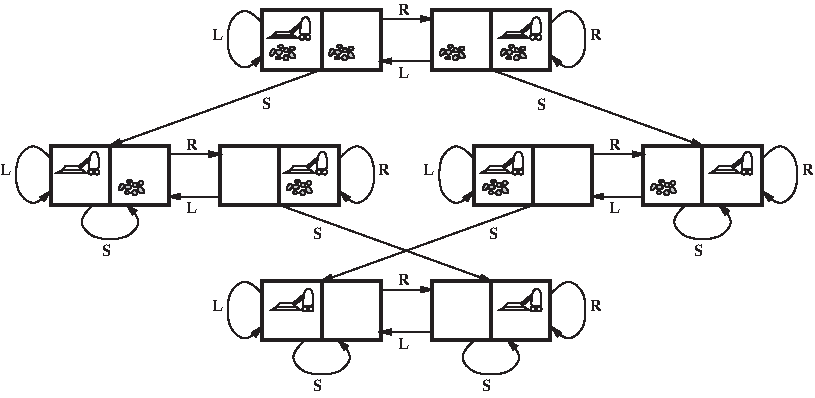
\includegraphics[width=\textwidth]{img/espaco-estados-aspirador}
	\caption{Espaço de estados para o mundo do aspirador de pó}
	\label{fig:espaco-estados-aspirador}
\end{figure}

\subsubsection{Quebra-cabeça de 8 peças}

O quebra-cabeça de 8 peças consiste em um tabuleiro de tamanho $3 \times 3$ com 8 peças numeradas e um espaço vazio. O objetivo é deslizar as peças pelo espaço vazio, de modo a ordená-las de forma crescente. A Figura~\ref{fig:quebra-cabeca-8-pecas} apresenta um exemplo do jogo com as peças embaralhadas e um exemplo com as mesmas ordenadas. É possível definir diferentes configurações de ordenação como estado objetivo.

\begin{itemize}
	\item \textbf{Estados:} cada estado especifica a posição de cada peça no tabuleiro e, consequentemente, o espaço vazio.
	
	\item \textbf{Estado inicial:} qualquer estado pode ser designado como estado inicial.
	
	\item \textbf{Função sucessor:} gera os estados válidos a partir das ações \textit{esquerda}, \textit{direita}, \textit{acima} e \textit{abaixo}, que podem er aplicadas à qualquer peça do jogo.
	
	\item \textbf{Teste de objetivo:} verifica se o estado corresponde à configuração desejada (conforme estado objetivo da Figura~\ref{fig:quebra-cabeca-8-pecas}).
	
	\item \textbf{Custo de caminho:} cada passo custa $1$, portanto, o custo do caminho é o número de passos realizados.
\end{itemize}

\begin{figure}[h]
	\centering
	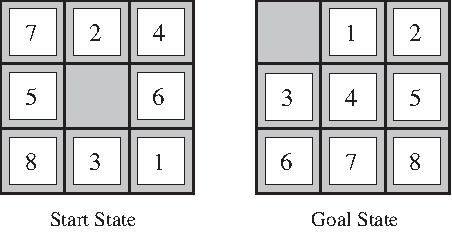
\includegraphics[width=0.5\textwidth]{img/quebra-cabeca-8-pecas}
	\caption{Exemplos de instâncias do quebra-cabeça de 8 peças}
	\label{fig:quebra-cabeca-8-pecas}
\end{figure}

\subsubsection{Problema das 8 rainhas}

O problema das 8 rainhas consiste em posicionar oito rainhas em um tabuleiro de xadrez\footnote{Existem variações com $n$ rainhas em tabuleiros $n \times n$.}, de tal forma que nenhuma rainha possa se atacar. Sabe-se que uma rainha pode atacar movimentando-se na linha, coluna ou na diagonal, um número qualquer de casas. A Figura~\ref{fig:exemplo-problema-8-rainhas} mostra um exemplo de posicionamento que não satisfaz o objetivo, pois as rainhas dos cantos superior esquerdo e inferior direito podem se atacar.

\begin{itemize}
	\item \textbf{Estados:} qualquer disposição de $0$ a $8$ rainhas no tabuleiro.
	
	\item \textbf{Estado inicial:} nenhuma rainha no tabuleiro.
	
	\item \textbf{Função sucessor:} colocar uma rainha em qualquer quadrado vazio.
	\begin{itemize}
		\item Uma abordagem que reduz o espaço de estados consiste em permitir a inserção de uma rainha apenas se o quadrado não estiver sob ataque.
	\end{itemize}
	
	\item \textbf{Teste de objetivo:} $8$ rainhas no tabuleiro sem que nenhuma possa se atacar.
	
	\item \textbf{Custo de caminho:} cada passo custa $1$, portanto, o custo do caminho é o número de passos realizados.
\end{itemize}

\begin{figure}[h]
	\centering
	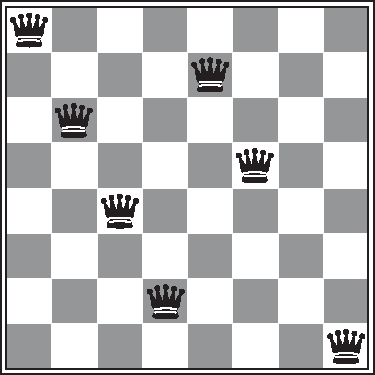
\includegraphics[width=0.5\textwidth]{img/exemplo-problema-8-rainhas}
	\caption{Exemplo de instância do problema das 8 rainhas}
	\label{fig:exemplo-problema-8-rainhas}
\end{figure}

\subsubsection{Roteamento}

Um dos problemas mais comuns é a definição de rotas, seja para veículos, pacotes em redes, aviões, etc. Consideremos o roteamento de veículos, tarefa similar à realizada por dispositivos GPS. A rede viária (mapa) é representada por um grafo, onde os vértices representam os pontos (cidades, por exemplo), enquanto os arcos representam caminhos de um ponto a outro (vias, por exemplo). A Figura~\ref{fig:grafo-cidades-roteamento} apresenta um grafo que representa o mapa de cidades da Romênia. O problema do roteamento consiste em encontrar o caminho de menor custo (também chamado de menor caminho ou caminho mínimo) entre uma origem e um destino. Por exemplo: qual o melhor caminho de \textit{Arad} até \textit{Bucharest}. Perceba que os arcos possuem valores associados, os quais representam o custo de viajar de um ponto a outro. Este grafo pode ser populado com diferentes custos, como distância, tempo de viagem, consumo de combustível, custo monetário, etc.

\begin{itemize}
	\item \textbf{Estados:} um estado é representado por um vértice (ou seja, uma cidade) acessível a partir do vértice de origem.
	
	\item \textbf{Estado inicial:} vértice de origem.
	
	\item \textbf{Função sucessor:} retorna o conjunto de vértices adjacentes do vértice atual. Ou seja, os vértices que possuam arcos com o vértice atual (comumente chamados de vizinhos).
	
	\item \textbf{Teste de objetivo:} verifica se o vértice atual é o vértice de destino.
	
	\item \textbf{Custo de caminho:} consiste no somatório dos custos dos arcos utilizados na rota.
\end{itemize}

\begin{figure}[h]
	\centering
	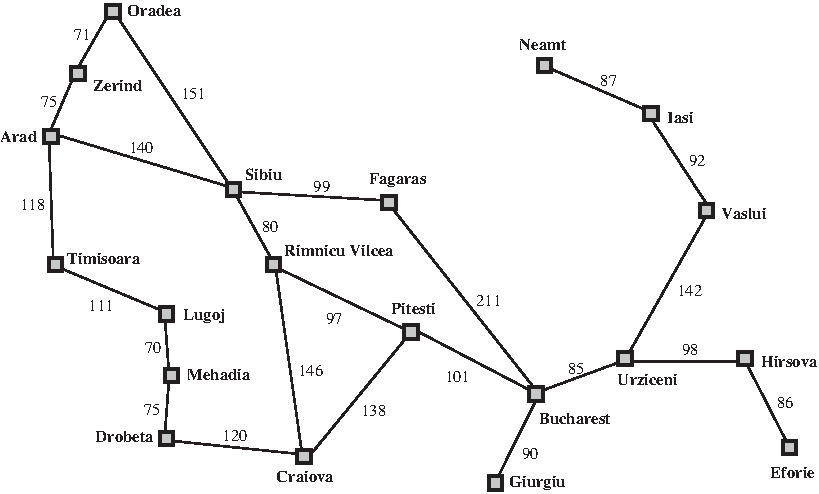
\includegraphics[width=\textwidth]{img/grafo-cidades-roteamento}
	\caption{Grafo das cidades da Romênia para o roteamento de veículos}
	\label{fig:grafo-cidades-roteamento}
\end{figure}

\subsection{Estratégia básica de busca}

A estratégia para solução destes problemas consiste em buscar no espaço de estados, algum estado que satisfaça o objetivo desejado (definido pelo teste de objetivo). Alguns problemas possuem uma única solução, isto é, um único estado que satisfaz o objetivo. Outros problemas, no entanto, possuem diferentes soluções, cada uma com seu respectivo custo. Finalmente, existem problemas para os quais qualquer estado é uma solução. Nos dois últimos casos, a estratégia de busca consiste em encontrar a melhor solução, ou seja, aquela que apresenta o menor custo. Esta solução é chamada de \textbf{solução ótima}.

Para realizar esta busca, deve-se partir do estado inicial e, através das ações disponíveis, caminhar para novos estados até encontrar um estado que satisfaça o objetivo. Para isso, criaremos uma \textbf{árvore de busca}, cujo nó raiz é o estado inicial, enquanto os nós filhos são os estados acessíveis mediante a realização das ações disponíveis. A Figura~\ref{fig:arvore-busca-roteamento} apresenta a árvore que busca uma rota entre as cidades de \textit{Arad} e \textit{Bucharest}, conforme o mapa apresentado na Figura~\ref{fig:grafo-cidades-roteamento}.

\begin{figure}[h]
	\centering
	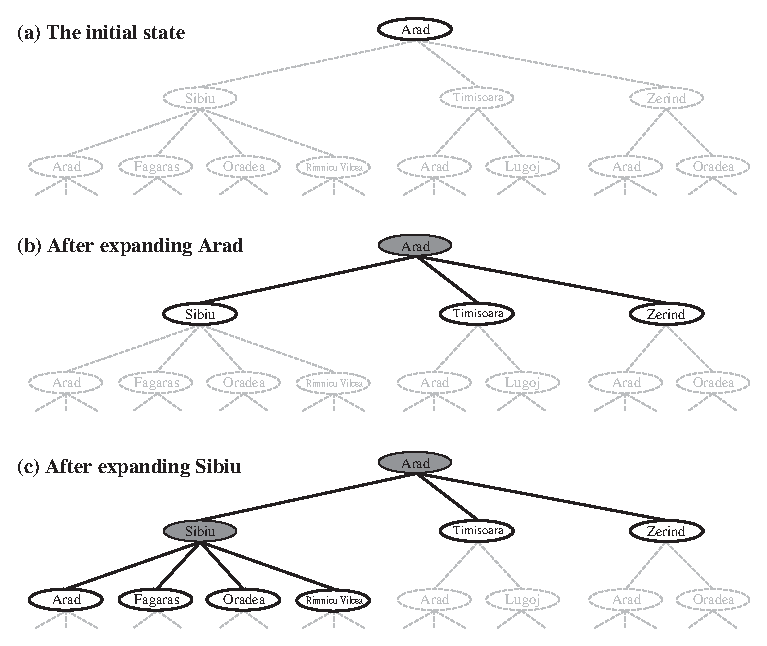
\includegraphics[width=\textwidth]{img/arvore-busca-roteamento}
	\caption{Árvore de busca para o problema de roteamento entre cidades da Romênia}
	\label{fig:arvore-busca-roteamento}
\end{figure}

A cada iteração, o algoritmo de busca deve verificar se o estado atual satisfaz o objetivo. No passo \texttt{(a)} da Figura~\ref{fig:arvore-busca-roteamento}, o estado atual consiste na cidade de origem, que é o estado inicial. Este nó é então expandido e os estados vizinhos são obtidos (através da função sucessor), o que é apresentado no momento \texttt{(b)}. O próximo estado é selecionado (\textit{Sibiu}). Como não satisfaz o objetivo, o nó é expandido \texttt{(c)}. A busca é executada até que o estado desejado (\textit{Bucharest}) é encontrado, ou quando se esgotam os vértices e a solução não é encontrada, caso em que o algoritmo deve retornar \texttt{falha}. O Algoritmo~\ref{alg:estrategia-basica-busca} apresenta um pseudocódigo para esta estratégia básica de busca.

\begin{algorithm}[h]
	\DontPrintSemicolon
	\Entrada{\textit{problema}, \textit{estratégia de seleção}}
	\Saida{\textit{solução}}
	
	\Inicio{
		\Repita{não haverem mais nós para expandir}{
			Seleciona um nó para expansão de acordo com \textit{\underline{estratégia de seleção}}\;
			\Se{nó contém um estado objetivo}{
				\Retorna{\textit{Solução correspondente}}
			}
			\Senao{
				Expandir o nó e adicionar os sucessores à árvore de busca\;
			}
		}
		\Retorna{\texttt{falha}}
	}
	
	\caption{Pseudocódigo para a estratégia básica de busca}
	\label{alg:estrategia-basica-busca}
\end{algorithm}

O que difere diferentes abordagens de busca é a estratégia de seleção de nós. Na Figura~\ref{fig:arvore-busca-roteamento}, o nó \textit{Arad} foi expandido para três filhos: \textit{Sibiu}, \textit{Timisoara} e \textit{Zerind}. No passo seguinte, o nó \textit{Sibiu} foi expandido para quatro novas cidades. Logo, o próximo passo poderia selecionar nós ainda não visitados do nível 2 ou do nível 3 da árvore. A estratégia de seleção de nós pode fazer com que o algoritmo tenha um desempenho melhor ou pior, de acordo com o problema tratado.

\textbf{Observação:} é importante diferenciar o \textit{espaço de estados} da \textit{árvore de busca}. No exemplo do roteamento, existem apenas 20 cidades no mapa e, portanto, 20 estados diferentes. Por outro lado, a árvore de busca é muito maior, pois consiste nos diferentes caminhos possíveis que podem ser feitos nesta rede. A árvore pode ser inclusive infinita, que é o caso deste problema de roteamento, uma vez que permite caminhos cíclicos\footnote{É claro que um bom algoritmo de busca deve evitar ciclos e, dessa forma, podar a árvore de busca.}. A árvore de busca é também chamada de \textbf{espaço de busca}.

\insertspace

Cada nó da árvore de busca é representado por uma estrutura de dados contendo:
\begin{itemize}
	\item \textbf{Estado:} o estado a que o nó corresponde.
	\item \textbf{Nó pai:} o nó da árvore que gerou esse nó.
	\item \textbf{Ação:} a ação que foi aplicada ao pai para gerar esse nó.
	\item \textbf{Custo:} o custo $g(n)$ do caminho desde o estado inicial até o nó.
	\item \textbf{Profundidade:} o número de passos ao longo do caminho, desde o estado inicial.
\end{itemize}

\insertspace

Finalmente, os diferentes algoritmos de busca são avaliados em função de quatro critérios:
\begin{itemize}
	\item \textbf{Completude:} o algoritmo oferece a garantia de encontrar uma solução, caso ela exista?
	
	\item \textbf{Otimalidade:} o algoritmo oferece a garantia de encontrar a solução ótima?
	
	\item \textbf{Complexidade de tempo:} quanto tempo ele leva para encontrar uma solução?
	
	\item \textbf{Complexidade de espaço:} quanta memória é necessária para executar a busca?
\end{itemize}

\insertspace

A complexidade em tempo e espaço é medida em função de alguns parâmetros do problema:
\begin{itemize}
	\item \textbf{Fator de ramificação $b$:} quantidade máxima de sucessores que qualquer nó pode gerar.
	
	\item \textbf{Profundidade $d$:} profundidade (nível) do nó meta mais próximo do inicial.
	
	\item \textbf{Comprimento máximo $m$:} comprimento máximo de qualquer caminho no espaço de estados.
\end{itemize}

\section{Algoritmos de busca cega}
\label{sec:busca-cega}

Os algoritmos de busca em árvore se dividem em duas categorias: busca cega e busca informada. A busca cega não possui qualquer informação sobre o problema, exceto sua definição. Com isso, ela tem que percorrer a árvore, verificando se o estado satisfaz o objetivo. Por outro lado, a busca informada consegue determinar o quanto um estado se aproxima do estado objetivo e, com isso, guiar a busca por ramos mais promissores da árvore, bem como descartar ramos ruins. Esta seção apresenta alguns algoritmos de busca cega que podem ser aplicados a qualquer problema\footnote{Ser aplicável a qualquer problema não significa que sua performance seja suficiente para resolver o problema.}.

\subsection{Busca em largura}

A busca em largura aplica uma estratégia onde o nó raiz é expandido, então todos os sucessores são expandidos, depois os sucessores dos sucessores, e assim por diante. Em outras palavras, todos os nós de uma dada profundidade na árvore de busca são expandidos, antes que todos os nós do nível seguinte sejam expandidos. A Figura~\ref{fig:busca-largura} mostra esta estratégia na exploração de uma árvore binária simples. Perceba que os nós \texttt{B} e \texttt{C} são expandidos antes dos nós \texttt{D}, \texttt{E}, \texttt{F} e \texttt{G}.

\begin{figure}[h]
	\centering
	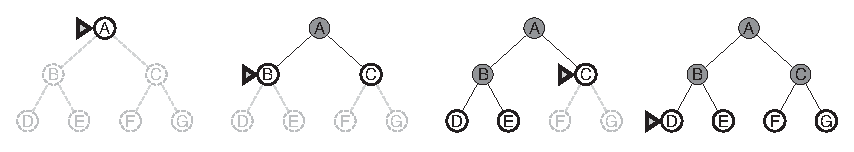
\includegraphics[width=\textwidth]{img/busca-largura}
	\caption{Busca em largura em uma árvore binária simples}
	\label{fig:busca-largura}
\end{figure}

A estratégia de busca em largura pode ser implementada utilizando uma estrutura de dados do tipo fila (FIFO -- \textit{first-in-first-out}) para armazenar os nós que ainda não foram expandidos. Em cada expansão, os filhos do nó expandido são inseridos na fila e, portanto, serão expandidos antes que seus filhos. O Algoritmo~\ref{alg:busca-largura} apresenta o pseudocódigo para uma busca em largura.

\begin{algorithm}[h]
	\DontPrintSemicolon
	\Entrada{\textit{nó inicial}}
	\Saida{\textit{solução}}
	
	\Inicio{
		Fila abertos $\gets \emptyset$\;
		abertos.add(inicial)\;
		\Enqto{abertos $\neq \emptyset$}{
			Nó atual $\gets$ abertos.remove()\;
			\Se{testeObjetivo(atual.estado)}{
				\Retorna{solução(atual)}
			}
			abertos.add(sucessores(atual))\;
		}
		
		\Retorna{\texttt{falha}}
	}
	
	\caption{Pseudocódigo para uma busca em largura}
	\label{alg:busca-largura}
\end{algorithm}

A busca em largura é \textit{completa}, pois sempre encontra uma solução caso ela exista. No entanto, esta solução não é garantidamente a melhor, portanto a busca não é ótima. Caso os custos sejam não-decrescentes à profundidade da solução, como um custo fixo igual para todas as ações, então a busca em largura é ótima, pois a melhor solução é a que se encontra no menor nível possível.

O problema da busca em largura é a complexidade de tempo e espaço. Considerando um fator de ramificação $b$ e uma profundidade $d$, cada nível $i$ expande $b^{i+1}$ nós da árvore de busca. No pior caso, a solução estará no último nó do nível $d$, o qual não será expandido. Portanto, no último nível a busca expande $b^{d+1} - b$ nós. Com isso, temos a complexidade\footnote{Esta complexidade pode ser diminuída para $O(b^d)$ se a verificação do nó possuir o estado objetivo ou não for realizada na sua geração, em vez de realizar na sua expansão.}
$$
b + b^2 + b^3 + \ldots + b^d + (b^{d+1} - b) = O(b^{d+1}).
$$

Considerando um fator de ramificação $b = 10$, que $10.000$ nós podem ser gerados por segundo e que um nó ocupa $1.000$\,bytes de espaço de armazenamento, a Tabela~\ref{tab:complexidade-busca-largura} mostra a quantidade de nós, o tempo gasto e a memória utilizada para uma busca em largura com diferentes valores de profundidade $d$. Muitos problemas apresentam estas características, o que nos leva a concluir que o tempo e a memória são os problemas críticos da busca em largura. Não temos computadores com memória na ordem de terabytes, por exemplo.

\begin{table}[h]
	\centering
	\setlength{\tabcolsep}{20pt}
	\begin{tabular}{rrrr}
		\hline
		\textbf{Profundidade} & \textbf{Nós} & \textbf{Tempo} & \textbf{Memória} \\
		\hline
		$2$ & $1100$ & $0,11$ segundo & $1$ megabyte \\
		$4$ & $111.100$ & $11$ segundos & $106$ megabytes \\
		$6$ & $10^7$ & $19$ minutos & $10$ gigabytes \\
		$8$ & $10^9$ & $31$ horas & $1$ terabyte \\
		$10$ & $10^{11}$ & $129$ dias & $101$ terabytes \\
		$12$ & $10^{13}$ & $35$ anos & $10$ petabytes \\
		$14$ & $10^{15}$ & $3.523$ anos & $1$ exabyte \\
		\hline
	\end{tabular}
	
	\caption{Desempenho de uma busca em largura em número de nós, tempo e espaço}
	\label{tab:complexidade-busca-largura}
\end{table}

\subsection{Busca em profundidade}

Diferente da anterior, a busca em profundidade sempre expande o nó mais profundo no conjunto de nós a serem expandidos. Esta estratégia é ilustrada na Figura~\ref{fig:busca-profundidade}, onde observamos que a busca desce os níveis na árvore até que o nó não tenha sucessores (\texttt{A} -- \texttt{B} -- \texttt{D} -- \texttt{H} $\ldots$). Quando os nós expandidos não tiverem mais sucessores a serem expandidos, eles não serão mais utilizados e podem ser removidos da memória, o que garante um consumo muito menor de espaço.

\begin{figure}[h]
	\centering
	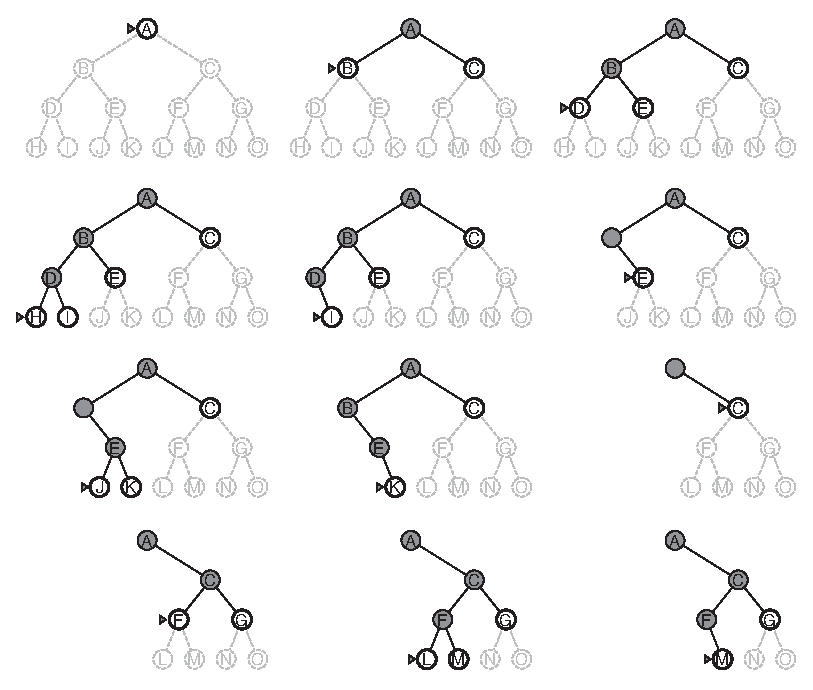
\includegraphics[width=\textwidth]{img/busca-profundidade}
	\caption{Busca em profundidade em uma árvore binária simples}
	\label{fig:busca-profundidade}
\end{figure}

Para implementar este comportamento, podemos utilizar uma estrutura de dados do tipo pilha (LIFO -- \textit{last-in-first-out}) para armazenar os nós que ainda não foram expandidos. Com isso, o último nó aberto é inserido na pilha e, portanto, será o primeiro a ser selecionado para expansão. O pseudocódigo para a busca em profundidade consiste em trocar a fila por uma pilha no Algoritmo~\ref{alg:busca-largura}. A busca em profundidade é completa somente se a árvore não é infinita, o que não é garantido em muitos problemas. Apesar de ser completa em árvores finitas, a busca não é ótima, pois uma solução sub-ótima pode ser encontrada em um primeiro ramo da árvore.

Como os ramos completamente explorados podem ser removidos da memória, a busca em profundidade só precisa armazenar um único caminho desde a raiz até um nó de folha, juntamente com os nós irmãos não expandidos restantes de cada nó no caminho. Considerando um fator de ramificação $b$ e uma profundidade máxima $m$, a busca em profundidade possui complexidade de espaço de $bm + 1 = O(bm)$. Considerando o mesmo cenário da Tabela~\ref{tab:complexidade-busca-largura} e supondo que nós da mesma profundidade do nó objetivo não têm sucessores, a busca em profundidade para $d = 12$ utilizaria $118$ kilobytes, ao invés de $10$ petabytes da busca em largura.

A complexidade de tempo de uma busca em profundidade depende da profundidade máxima $m$ da árvore de busca. Logo, podemos definir a complexidade de tempo como $O(b^m)$. Caso a árvore seja infinita (por conta de estados repetidos), a busca não terminaria sua execução e algum mecanismo de poda deve ser adotado.

\subsection{Busca em profundidade limitada}

Uma abordagem comum é limitar o nível de profundidade, gerando uma \textbf{busca em profundidade limitada}. Definindo um limite de profundidade $l$, nós no nível $l$ serão tratados como se não tivessem sucessores. A busca passa a ser incompleta se $l < d$, o que é um fator importante uma vez que na maioria dos problemas não se conhece $d$ \textit{a priori}. O Algoritmo~\ref{alg:busca-profundidade-limitada} apresenta um pseudocódigo para uma busca em profundidade limitada.

\begin{algorithm}[h]
	\DontPrintSemicolon
	\Entrada{\textit{nó inicial}, \textit{limite de profundidade} $l$}
	\Saida{\textit{solução}}
	
	\Inicio{
		Pilha abertos $\gets \emptyset$\;
		abertos.add(inicial)\;
		\Enqto{abertos $\neq \emptyset$}{
			Nó atual $\gets$ abertos.remove()\;
			\Se{testeObjetivo(atual.estado)}{
				\Retorna{solução(atual)}
			}
			
			\Se{atual.profundidade $< l$}{
				abertos.add(sucessores(atual))\;
			}
		}
		
		\Retorna{\texttt{falha}}
	}
	
	\caption{Pseudocódigo para uma busca em profundidade limitada}
	\label{alg:busca-profundidade-limitada}
\end{algorithm}

Mesmo com a seleção de um limite $l > d$, a busca em profundidade limitada não garante otimalidade. No entanto, suas complexidades de tempo e espaço são ainda menores, pois a exploração é feita em parte da árvore de busca. A busca em profundidade tradicional pode ser vista como uma busca em profundidade limitada com $l = \infty$.

A complexidade da busca é medida, obviamente, em função do limite $l$. A complexidade de tempo é é $O(b^l)$, enquanto a complexidade de espaço é $O(bl)$.

\subsection{Busca em profundidade iterativa}

Uma vez que não se conhece \textit{a priori} um valor adequado para o limite de profundidade $l$, a busca em profundidade iterativa tenta encontrar o melhor valor durante a sua execução. Para isso, o algoritmo aumenta gradativamente o valor de $l$, iniciando por 0 e incrementando em 1, até encontrar uma solução, que ocorre quando $l = d$. Em outras palavras, esta abordagem combina a busca em profundidade com a busca em largura. O Algoritmo~\ref{alg:busca-profundidade-iterativa} apresenta um pseudocódigo para a busca em profundidade iterativa.

\begin{algorithm}[h]
	\DontPrintSemicolon
	\Entrada{\textit{nó inicial}}
	\Saida{\textit{solução}}
	
	\Inicio{
		\Para{$l \gets 0$ \textbf{até} $\infty$}{
			solução $\gets$ BUSCA-PROFUNDIDADE-LIMITADA(\textit{inicial}, $l$)\;
			\Se{solução $\neq$ \texttt{falha}}{
				\Retorna{solução}
			}
		}
	}
	
	\caption{Pseudocódigo para uma busca em profundidade iterativa}
	\label{alg:busca-profundidade-iterativa}
\end{algorithm}

\begin{figure}[h]
	\centering
	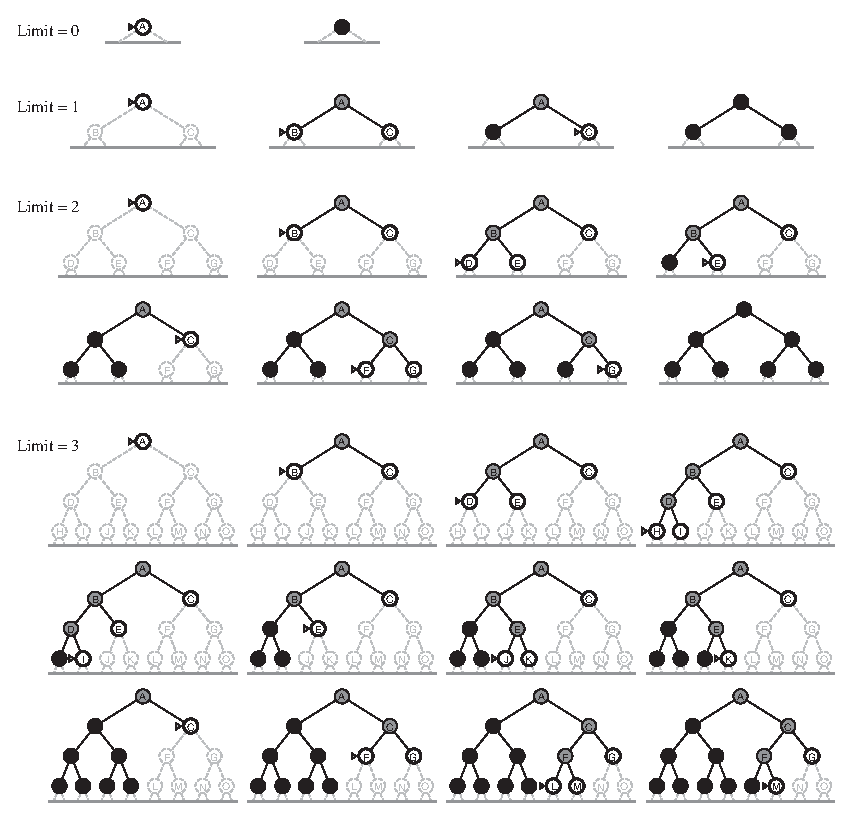
\includegraphics[width=0.995\textwidth]{img/busca-profundidade-iterativa}
	\caption{Busca em profundidade iterativa em uma árvore binária simples}
	\label{fig:busca-profundidade-iterativa}
\end{figure}

%\clearpage

A Figura~\ref{fig:busca-profundidade-iterativa} ilustra o funcionamento de uma busca em profundidade iterativa. No limite 0, apenas a raiz é analisada. No limite 1, a raiz é expandida e o primeiro nível é analisado. Quando os níveis aumentam, a estratégia de seleção de nós é idêntico ao de uma busca em profundidade, mas os nós mais rasos já foram explorados em iterações anteriores. Logo, este algoritmo faz uma busca em largura sem a necessidade de manter os nós em memória, isto é, utiliza os benefícios de ambas abordagens.

A busca em profundidade iterativa é completa, pois encontra uma solução, caso ela exista. Da mesma forma que ocorre na busca em largura, esta abordagem é ótima se o custo for não-decrescente (uniforme, por exemplo) ao nível de profundidade. Apesar de parecer desperdício gerar os mesmos estados repetidamente em diferentes iterações, o maior número de estados (em maiores níveis de profundidade) são gerados poucas vezes. De fato, o nível $d$ é gerado uma só vez, o nível $d+1$ é gerado duas vezes, e assim por diante. Logo, temos a seguinte complexidade de tempo:
$$
(d)b + (d - 1)b^2 + \ldots + (1)b^d = O(b^d).
$$

Comparando a complexidade da busca em profundidade iterativa ($O(b^d)$) com a busca em largura ($O(b^{d+1} - b)$), percebemos que a busca em largura é mais complexa, pois gera alguns nós de profundidade $d+1$. Como resultado, a busca em profundidade iterativa é mais rápida e, na maioria dos casos, é o algoritmo de busca preferido quando existe um espaço de busca grande e a profundidade da solução não é conhecida.

\subsection{Busca bidirecional}

A ideia da busca bidirecional é executar duas buscas em paralelo. A primeira busca é simples e explora os nós a partir do estado inicial, conforme visto até o momento. A segunda busca utiliza o estado objetivo como estado inicial, explorando a árvore de busca a partir dele. Quando as duas buscas encontrarem um nó em comum, o caminho desde o estado inicial até o estado objetivo é traçado. A ideia geral desta busca é expressa na Figura~\ref{fig:busca-bidirecional}. A motivação desta busca é que $b^{d/2} + b^{d/2} < b^d$. Isto é, a soma das áreas dos dois círculos é menor que a área de um grande círculo partindo do estado inicial até encontrar o estado objetivo. 

\begin{figure}[h]
	\centering
	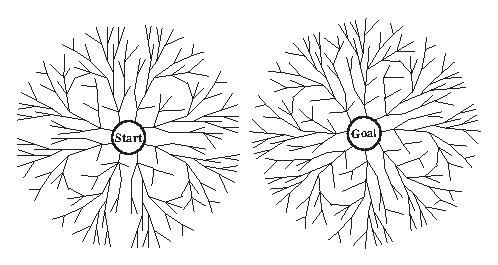
\includegraphics[width=0.8\textwidth]{img/busca-bidirecional}
	\caption{Ideia geral da busca bidirecional}
	\label{fig:busca-bidirecional}
\end{figure}

No momento da geração de nós, cada busca verifica se os nós não estão na lista de nós a serem explorados da outra busca. Em caso positivo, é encontrada uma solução. Se um problema possui solução na profundidade $d = 6$ e são executadas duas buscas em largura, então no pior caso cada busca expande todos os nós da profundidade 3, exceto um. Para $b = 10$, isso significa $22.200$ nós gerados, em comparação com $11.111.100$ nós gerados por uma busca em largura.

Como a busca de um nó na outra árvore pode ser feito em tempo constante, a complexidade de tempo de uma busca bidirecional é $O(b^{d/2})$. A complexidade de espaço é definida pelo armazenamento de pelo menos uma das árvores em memória, o que leva à mesma complexidade de $O(b^{d/2})$. Caso ambas as buscas forem em largura e os passos tiverem custo uniforme, então a busca é completa e ótima. Diferentes buscas podem sacrificar uma ou as duas características.

A dificuldade deste método está na exploração do espaço de estados a partir do estado objetivo. Nem sempre é possível determinar os predecessores de um estado, ou seja, os estados-pai possíveis. Isso faz com que a busca bidirecional não possa ser aplicada a qualquer problema.

\subsection{Comparação entre as abordagens}

A Tabela~\ref{tab:comparacao-busca-cega} resume a avaliação dos diferentes métodos de busca cega apresentados neste capítulo.

\begin{table}[h]
	\centering
	\small
	\begin{tabular}{l|L{2.5cm}L{2.5cm}L{2.5cm}L{2.5cm}}
		\hline
		\textbf{Busca} & \textbf{Completa} & \textbf{Ótima} & \textbf{Tempo} & \textbf{Espaço} \\
		\hline
		
		Largura & Sim & Sim\tablefootnote{Desde que o custo do passo seja não-decrescente ao nível de profundidade.} & $O(b^{d+1})$ & $O(b^{d+1})$ \\
		
		Profundidade & Não & Não & $O(b^m)$ & $O(bm)$ \\
		
		Profundidade limitada & Não & Não & $O(b^l)$ & $O(bl)$ \\
		
		Profundidade iterativa & Sim & Sim\tablefootnote{Desde que o custo do passo seja não-decrescente ao nível de profundidade.} & $O(b^d)$ & $O(bd)$ \\
		
		Bidirecional & Sim\tablefootnote{Desde que ambas as buscas sejam em largura.} & Sim\tablefootnote{Se ambas as buscas sejam em largura e os custos dos passos sejam todos idênticos.} & $O(b^{d/2})$ & $O(b^{d/2})$ \\
		\hline
		
	\end{tabular}
	\caption{Comparação de diferentes estratégias de busca cega}
	\label{tab:comparacao-busca-cega}
\end{table}

\section{Algoritmos de busca informada}

A Seção~\ref{sec:busca-cega} apresentou alguns algoritmos de busca que não possuem nenhuma informação do problema, exceto sua definição. Com isso, estes métodos exploram a árvore de busca, verificando cada estado gerado seguindo alguma estratégia genérica. Estes algoritmos não são aplicáveis a problemas reais, pois eles comumente são muito grandes e complexos. Com isso, a busca cega não consegue encontrar a solução em tempo razoável com os recursos de memória existentes. Para resolver este problema, podemos utilizar informações do problema para guiar a busca, explorando regiões promissoras da árvore de busca. Estes algoritmos são classificados como busca informada.

Para isso, utilizaremos uma \textbf{função de avaliação} $f(n)$ que determina o custo de um nó da árvore de busca. Dessa forma, a busca pode selecionar os nós de menor custo para exploração. Esta função é definida como:
$$
f(n) = g(n) + h(n),
$$
em que $n$ é um nó da árvore de busca, $g(n)$ é o \textbf{custo do caminho} desde o nó inicial até $n$ e $h(n)$ é chamada \textbf{função heurística}.

O custo do caminho é armazenado em cada nó da árvore e é proveniente do custo da execução das ações que levam até um determinado estado, conforme apresentado nas seções anteriores. A função heurística deve ser determinada pelo projetista e mede (ou estima) a distância do nó atual ($n$) até o nó objetivo.

\subsection{Busca uniforme}

Uma primeira abordagem consiste em selecionar o nó cujo caminho até ele seja o menor possível. Em outras palavras, consideramos $f(n) = g(n)$. Esta abordagem é chamada de busca uniforme e garante a otimalidade, desde que os custos sejam positivos. O Algoritmo~\ref{alg:busca-informada} mostra o pseudocódigo para uma busca informada, onde a lista de nós abertos é ordenada em função de $f(n)$ (linha 2), isto é, selecionando sempre o menor valor (linha 5).

\begin{algorithm}[h]
	\DontPrintSemicolon
	\Entrada{\textit{nó inicial}}
	\Saida{\textit{solução}}
	
	\Inicio{
		ListaOrdenada abertos $\gets \emptyset$\;
		abertos.add(inicial)\;
		\Enqto{abertos $\neq \emptyset$}{
			Nó atual $\gets$ abertos.removeFirst()\;
			\Se{testeObjetivo(atual.estado)}{
				\Retorna{solução(atual)}
			}
			abertos.add(sucessores(atual))\;
		}
		
		\Retorna{\texttt{falha}}
	}
	
	\caption{Pseudocódigo para uma busca informada}
	\label{alg:busca-informada}
\end{algorithm}

A busca uniforme garante que, quando um nó é selecionado para expansão, foi encontrado o menor caminho até ele. Ao retomar o problema do roteamento entre as cidades da Romênia (Figura~\ref{fig:grafo-cidades-roteamento-2}), consideremos a tarefa de ir de \textit{Sibiu} para \textit{Bucharest}. Ao expandir o nó \textit{Sibiu}, são abertos os nós \textit{Fagaras}, com custo de 99 e \textit{Rimnicu Vilcea}, com custo de 80. O nó \textit{Rimnicu Vilcea} é selecionado para expansão, adicionando as cidades de \textit{Pitesti} (custo de $80 + 97 = 177$) e \textit{Craiova} (custo de $80 + 146 = 226$). Com isso, o menor custo passa a ser \textit{Fagaras}, que é selecionado, abrindo o nó de \textit{Bucharest}, com custo de $99 + 211 = 310$. Apesar de este ser o nó destino, existem caminhos em aberto que possuem custo menor que 310. Ou seja, pode ser que encontremos um caminho com custo menor que o encontrado até o momento. Por isso, a busca uniforme só termina quando garantidamente não existe um caminho de menor custo.

Seguindo a busca, o nó de menor custo é \textit{Pitesti} (custo de $80 + 97 = 177$), que é selecionado, abrindo o nó \textit{Bucharest} com custo de $177 + 101 = 278$. Perceba que encontramos um caminho com menor custo que o anterior. Além disso, os caminhos em aberto possuem todos um custo maior que 278. Logo, o próximo nó selecionado é \textit{Bucharest} e garantimos que o caminho de menor custo foi encontrado.

\begin{figure}[h]
	\centering
	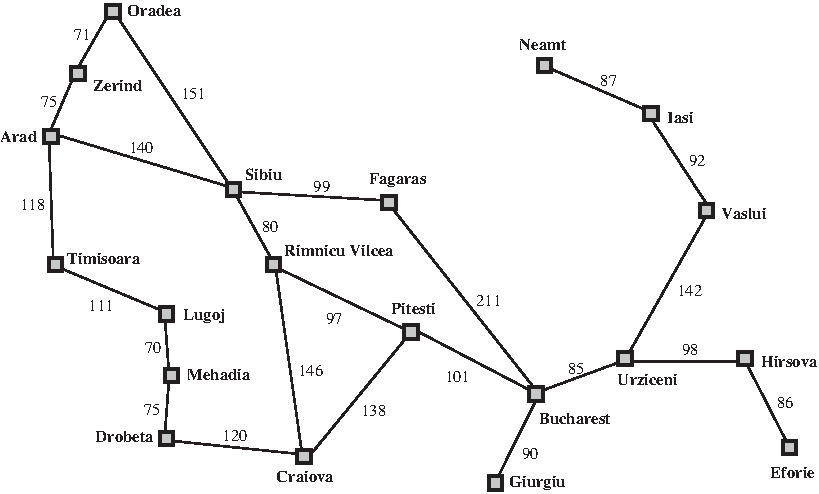
\includegraphics[width=\textwidth]{img/grafo-cidades-roteamento}
	\caption{Grafo das cidades da Romênia para o roteamento de veículos}
	\label{fig:grafo-cidades-roteamento-2}
\end{figure}

Apesar de ser um algoritmo ótimo quando os custos são positivos, esta estratégia demora para convergir, pois não descarta nenhum caminho (ramo da árvore) até ter a certeza de que não pode produzir um caminho melhor. Por exemplo, uma grande sequência de passos pequenos sempre será explorada até descobrir que adiante existe um passo gigante que elimina este caminho da solução. Além disso, se tivermos algum arco com custo igual a zero, a busca pode ficar presa em um laço infinito ao selecionar sempre o mesmo nó para expansão.

\subsection{Busca gulosa}

A busca gulosa (\textit{greedy search}) é também conhecida por busca gulosa de melhor escolha e utiliza a função heurística como guia para uma busca mais rápida. Ou seja, a busca gulosa define $f(n) = h(n)$ e expande o nó que apresenta o menor $f(n)$, até encontrar a solução. Seu funcionamento é o mesmo apresentado no Algoritmo~\ref{alg:busca-informada}, considerando a nova função $f(n)$. Em resumo, é a estratégia contrária à busca uniforme, pois ao invés de usar o custo do caminho do início até o nó $n$, utiliza o custo estimado do nó $n$ até o objetivo. 

Consideremos o problema de roteamento entre as cidades da Romênia (Figura~\ref{fig:grafo-cidades-roteamento-2}), partindo de \textit{Arad} com destino em \textit{Bucharest}. Como a busca não conhece o grafo completo, não é possível utilizar a distância real de cada cidade até o destino \textit{Bucharest}. Portanto, consideremos como função heurística $h(n)$ a distância em linha reta de cada cidade até \textit{Bucharest}. Estes valores são apresentados na Tabela~\ref{tab:distancias-cidades-bucareste}. Exemplo: $h($\textit{Arad}$) = 366$.

\begin{table}[b!]
	\centering
	\begin{tabular}{lr|lr}
		\hline
		\textbf{Cidade} & \textbf{Distância} & \textbf{Cidade} & \textbf{Distância}\\
		\hline
		Arad & 366 & Mehadia & 241 \\
		Bucharest & 0 & Neamt & 234 \\
		Craiova & 160 & Oradea & 380 \\
		Drobeta & 242 & Pitesti & 100 \\
		Eforie & 161 & Rimnicu Vilcea & 193 \\
		Fagaras & 176 & Sibiu & 253 \\
		Giurgiu & 77 & Timisoara & 329 \\
		Hirsova & 151 & Urzineci & 80 \\
		Iasi & 226 & Vaslui & 199 \\
		Lugoj & 244 & Zerind & 374 \\
		\hline
	\end{tabular}
	
	\caption{Distância de cada cidade até Bucharest -- para função heurística}
	\label{tab:distancias-cidades-bucareste}
\end{table}

O funcionamento da busca gulosa para o problema de roteamento na Romênia é ilustrado na Figura~\ref{fig:execucao-busca-gulosa}. O nó inicial é \textit{Arad}, que possui $f(n) = h(n) = 366$. A expansão desse nó gera os nós \textit{Sibiu}, \textit{Timisoara} e \textit{Zerind}. A busca seleciona o nó \textit{Sibiu}, pois apresenta menor $f(n)$. Sua expansão gera mais quatro nós, dos quais \textit{Fagaras} é selecionado, pois apresenta o menor $f(n)$. Finalmente, a expansão de \textit{Fagaras} gera \textit{Bucharest}, que é o nó objetivo. A busca encontra, portanto, a solução para o problema.

\insertspace

\begin{figure}[h]
	\centering
	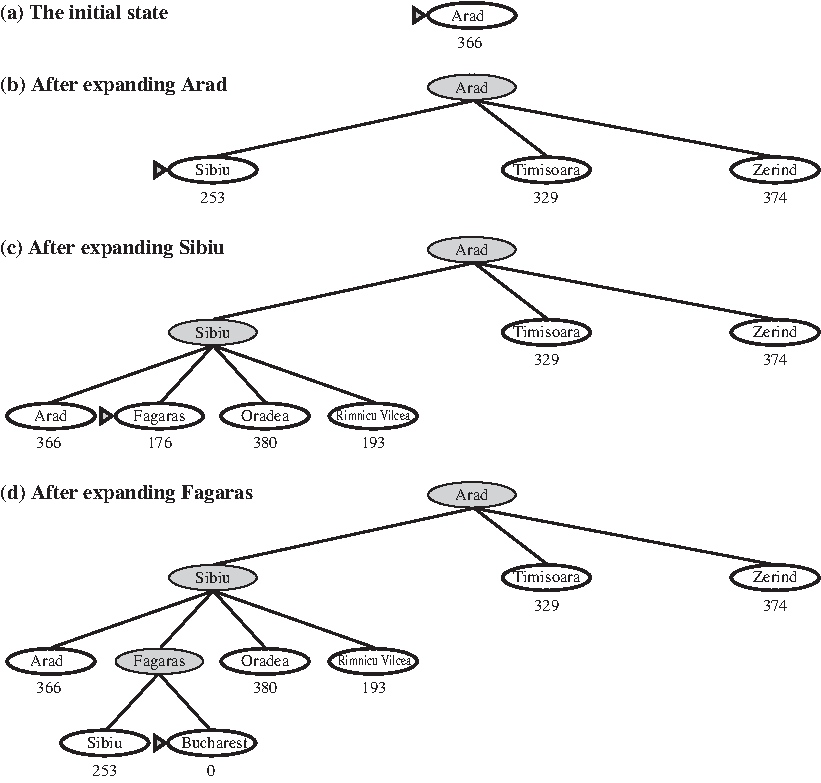
\includegraphics[width=\textwidth]{img/execucao-busca-gulosa}
	\caption{Execução de uma busca gulosa para roteamento entre cidades da Romênia}
	\label{fig:execucao-busca-gulosa}
\end{figure}

A busca gulosa não é ótima. Perceba que existe um caminho de menor custo (\textit{Arad} -- \textit{Sibiu} -- \textit{Rimnicu Vilcea} -- \textit{Pitesti}). Por conta da gulosidade (ambição) da busca, ela ignora regiões da árvore de busca que parecem ser mais custosas mas levam a uma solução melhor. Além disso, a busca não é completa caso nenhuma estratégia de poda seja utilizada, pois mesmo em espaços de estados finitos a árvore de busca pode ser infinita (ciclos) e a busca nunca encontra uma solução\footnote{Mesma situação da busca em profundidade.}.

\subsection{Busca A*}

A busca A* (A estrela) utiliza simultaneamente as estratégias adotadas nas buscas uniforme e gulosa. Isto é, considera o custo do caminho e o custo futuro estimado. Com isso, a busca A* considera caminhos com menor expectativa de custo, mas evita caminhos que já estejam muito caros. A função $f(n) = g(n) + h(n)$ pode ser vista como o custo estimado da solução que passa pelo nó $n$. Com isso, se garante a otimalidade da busca uniforme, mas a árvore não precisa ser explorada exaustivamente. O funcionamento da busca A* é idêntico ao Algoritmo~\ref{alg:busca-informada} com a lista de nós ordenada pela nova função $f(n)$.

A execução do algoritmo de busca A* para o roteamento entre cidades da Romênia é apresentada na Figura~\ref{fig:execucao-busca-a-estrela}. Observe que a busca considera $f(n) = g(n) + h(n)$ para a seleção de vértices. A cidade de \textit{Bucharest} aparece como candidata à seleção da etapa \texttt{(e)}. No entanto, o caminho passando por \textit{Rimnicu Vilcea} -- \textit{Pitesti} parece mais promissor, pois possui menor $f(n)$. Logo, a busca A* seleciona o nó \textit{Pitesti}, encontrando um caminho mais curto.

\begin{figure}[h]
	\centering
	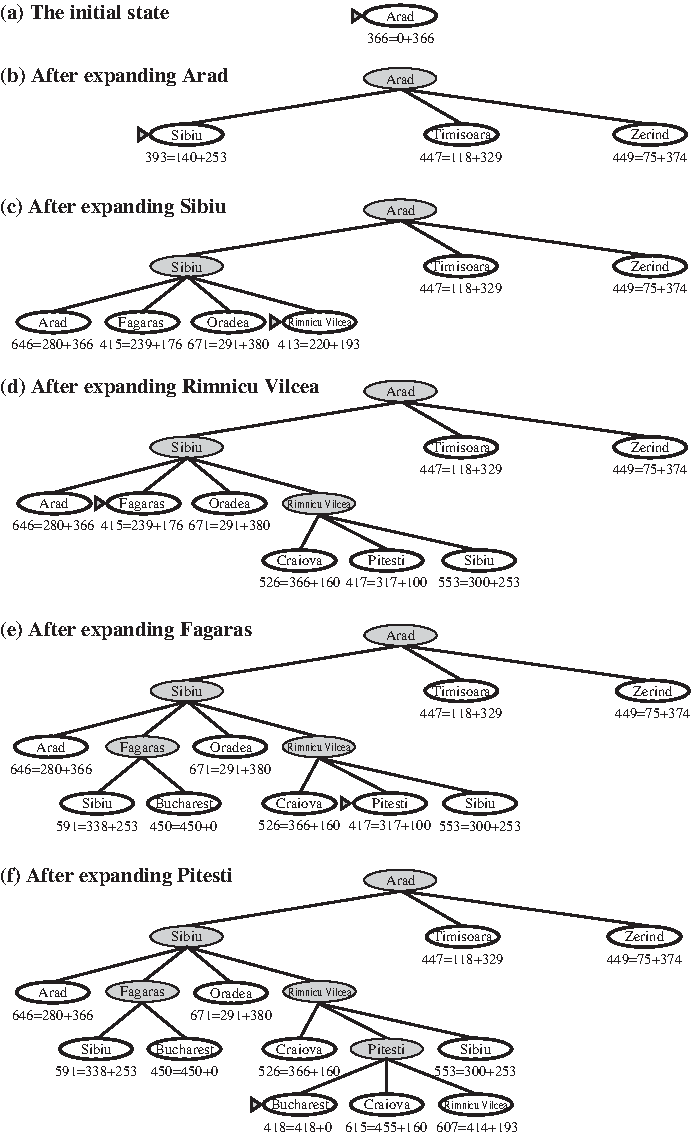
\includegraphics[width=0.9\textwidth]{img/execucao-busca-a-estrela}
	\caption{Execução de uma busca A* para roteamento entre cidades da Romênia}
	\label{fig:execucao-busca-a-estrela}
\end{figure}

A busca A* é completa, pois evita ciclos, uma vez que considera o custo passado. Obviamente, esta condição é verdadeira somente se os custos nas arestas forem maiores que zero. A busca A* é também ótima, desde que a função heursítica $h(n)$ seja \textbf{admissível}. A função é admissível caso ela \textbf{nunca superestime} o custo para alcançar o objetivo (dizemos que a função deve ser otimista). Em outras palavras, o custo estimado pela função heurística deve ser menor ou igual ao custo real. Caso a busca superestime o custo, ela pode descartar a solução ótima por calcular um custo superior ao real.

No caso do roteamento entre cidades da Romênia, a função heurística é admissível, pois a distância entre duas cidades não pode ser menor que a distância de uma linha reta entre elas. Logo, $h(n)$ não pode ser uma superestimativa e a busca é ótima para este problema.

\section{Recursos disponíveis}

Existem vários sites e aplicações com o objetivo de ensinar e esclarecer os algoritmos de busca em árvores, como o Visualgo~\footnote{\url{https://visualgo.net/en}} e as ferramentas disponibilizadas pelo professor David Galles~\footnote{\url{https://www.cs.usfca.edu/~galles/visualization/Algorithms.html}}. Além disso, a ferramenta Web de \textit{Graph Searching}~\footnote{\url{http://aispace.org/search}} da plataforma AIspace~\footnote{\url{http://www.aispace.org}}. Finalmente, existem bibliotecas que implementam os algoritmos de busca em árvore, como a disponibilizada pelo professor Jomi Hübner~\footnote{\url{http://jomi.das.ufsc.br/ia/busca/buscaJava/index.html}}.

\clearpage

\section{Exercícios}

\resetexercisenumbering

\begin{exercise}
Defina com suas próprias palavras os seguintes termos: estado, espaço de estados, árvore de busca, nó de busca, objetivo, ação, modelo de transição e fator de ramificação.
\end{exercise}

\begin{exercise}
Qual é a diferença entre um estado do mundo, uma descrição do estado e um nó de busca? Por que é útil essa distinção?
\end{exercise}

\begin{exercise}
Suponha que dois amigos vivam em cidades de locais diferentes no mapa da Romênia. Podemos mover cada amigo de cada vez simultaneamente para uma cidade vizinha no mapa. A quantidade de tempo necessário para se deslocar da cidade $i$ à vizinha $j$ é igual à distância $d(i,j)$ entre as cidades, mas a cada vez que o amigo chega primeiro deve
esperar até o outro chegar (e telefonar para o primeiro do celular) antes que comece a próxima vez de se movimentarem. Queremos que os dois amigos se encontrem o mais rápido possível.

\begin{enumerate}[a.]
	\item Escreva uma formulação detalhada para esse problema de busca (será útil definir alguma notação formal).
	
	\item Seja $D(i,j)$ a distância em linha reta entre as cidades $i$ e $j$. Qual das seguintes funções heurísticas é admissível? (i) $D(i,j)$, (ii) $2 \cdot D(i,j)$ e (iii) $D(i,j) / 2$.
	
	\item Há mapas completamente conectados para os quais não existe solução?
	
	\item Há mapas em que todas as soluções requerem que um amigo visite a mesma cidade duas vezes?
\end{enumerate}
\end{exercise}

\begin{exercise}
Forneça uma formulação completa do problema para cada um dos seguintes itens. Escolha a formulação suficientemente precisa para ser implementada.

\begin{enumerate}[a.]
	\item Usando apenas 4 cores, colorir um mapa plano de tal forma que duas regiões adjacentes não tenham a mesma cor.
	
	\item Um macaco com 30 cm está em uma sala onde tem algumas bananas suspensas em um teto de 80\,cm. Ele gostaria de pegar as bananas. A sala contém dois engradados móveis e escaláveis com 30\,cm de altura que podem ser empilhados.
	
	\item Existem três jarras que medem 12, 8 e 3 galões e uma torneira de água. As jarras podem ser enchidas ou esvaziadas uma da outra ou para o chão. Medir exatamente um galão, somente com essas operações.
\end{enumerate}
\end{exercise}

\begin{exercise}
Este exercício explora a aplicação dos algoritmos de busca quando existem custos negativos nos caminhos.

\begin{enumerate}[a.]
	\item Suponha que as ações possam ter custos negativos arbitrariamente grandes; explique por que essa possibilidade forçaria qualquer algoritmo ótimo a explorar todo o espaço de estados.
	
	\item Ajudaria se insistíssemos no fato de que os custos dos passos devem ser maiores ou iguais a alguma constante negativa $c$?
	
	\item Suponha que um conjunto de ações forme um laço no espaço de estados de modo que a cada execução dessas ações em alguma ordem não resulte em mudança no estado. Se todas essas ações tiverem custo negativo, qual será a implicação desse fato sobre o comportamento ótimo de um agente em tal ambiente?
	
	\item É possível imaginar facilmente ações com custo negativo alto, até mesmo em domínios como o de roteamento. Por exemplo, alguns trechos da estrada poderiam ter belas paisagens que superem de longe os custos normais em termos de tempo e combustível. Explique, em termos precisos, dentro do contexto de busca em espaços de estados, por que os seres humanos não dirigem indefinidamente em ciclos por belos cenários e explique como definir o espaço de estados e ações para roteamento, de forma que agentes artificiais também possam evitar ciclos repetitivos.
\end{enumerate}
\end{exercise}

\begin{exercise}
O problema de missionários e canibais é normalmente enunciado como a seguir. Três missionários e três canibais estão em um lado de um rio, juntamente com um barco que pode levar uma ou duas pessoas. Descubra um meio de fazer todos atravessarem o rio sem deixar que um grupo de missionários de um lado fique em número menor que o número de canibais nesse mesmo lado do rio.

\begin{enumerate}[a.]
	\item Formule o problema precisamente, fazendo apenas as especificações necessárias para assegurar uma solução válida. Faça um diagrama do espaço de estados completo.
	
	\item Implemente e resolva o problema de forma ótima, utilizando um algoritmo de busca apropriado. É uma boa ideia verificar a existência de estados repetidos?
	
	\item Por que você imagina que as pessoas têm dificuldades para resolver esse quebra-cabeça, considerando que o espaço de estados é tão simples?
\end{enumerate}
\end{exercise}

\begin{exercise}
Uma ação tal como \textit{Ir para Sibiu} consiste realmente em uma longa sequência de ações mais refinadas: ligar o carro, soltar o freio, acelerar para a frente, etc. Ter ações compostas desse tipo reduz o número de passos em uma sequência de soluções, reduzindo assim o tempo de busca. Suponha que tomemos essa lógica ao extremo, construindo ações supercompostas de todas as sequências possíveis de ações \textit{Ir}. Assim, cada instância do problema é resolvida por uma única ação supercomposta, como \textit{Ir para Sibiu -- Ir para Rimnicu Vilcea -- Ir para Pitesti -- Ir para Bucareste} . Explique como a busca trabalharia nessa formulação. Essa é uma abordagem prática para acelerar a resolução do problemas?
\end{exercise}

\begin{exercise}
Quais das seguintes alternativas são falsas e quais são verdadeiras? Explique suas respostas.

\begin{enumerate}[a.]
	\item A busca em profundidade sempre expande pelo menos tantos nós quanto a busca A* com uma heurística admissível.
	
	\item $h(n) = 0$ é uma heurística admissível para o quebra cabeças de 8 peças.
	
	\item Em robótica, A* não é útil porque as percepções, estados e ações são contínuas.
	
	\item A busca em largura é completa mesmo se os custos de passos iguais a zero forem permitidos.
	
	\item Assuma que a torre pode se mover em um tabuleiro de xadrez qualquer quantidade de quadrados em linha reta, verticalmente ou horizontalmente, mas não pode pular sobre as peças. A distância de Manhattan é uma heurística admissível para o problema de movimentar a torre do quadrado \texttt{A} para o \texttt{B} no menor número de movimentos.
\end{enumerate}
\end{exercise}

\begin{exercise}
Considere um espaço de estados onde o estado inicial é o número $1$ e cada estado $k$ tem dois sucessores: números $2k$ e $2k + 1$.

\begin{enumerate}[a.]
	\item Represente a porção do espaço de estados para os estados de 1 a 15.
	
	\item Suponha que o estado objetivo seja 11. Liste a ordem em que os nós serão visitados pela busca em largura, busca em profundidade limitada com o limite 3 e busca de aprofundamento iterativo.
	
	\item Como a busca bidirecional funcionaria nesse problema? Qual é o fator de ramificação em cada direção?
	
	\item A resposta ao item \texttt{(c)} sugere uma reformulação do problema que permitiria resolver o problema de ir do estado 1 para um determinado estado objetivo com quase nenhuma busca?
	
	\item Chame a ação que vai de $k$ para $2k$ de Esquerda e a ação de $k$ que vai para $2k + 1$ de Direita. É possível encontrar um algoritmo que devolva a solução desse problema absolutamente sem nenhuma busca?
\end{enumerate}
\end{exercise}

\begin{exercise}
Faça passo a passo a execução de uma busca A* aplicada para o problema de chegar a \textit{Bucharest} a partir de \textit{Lugoj} utilizando a distância heurística em linha reta. Isto é, mostre a sequência de nós que o algoritmo vai considerar e a pontuação $f$, $g$ e $h$ para cada nó.
\end{exercise}

\begin{exercise}
Considere o problema do quebra cabeça de 8 peças, formalizado neste capítulo. Implemente os seguintes algoritmos de busca:

\begin{itemize}
	\item Busca em largura
	\item Busca em profundidade
	\item Busca A*
\end{itemize}

Faça um relatório mostrando o desempenho de cada algoritmo: custo do caminho encontrado até a solução, quantidade de vértices visitados, quantidade de vértices armazenados na memória a cada iteração e tempo de execução.
\end{exercise}

\begin{exercise}
Utilize a biblioteca de algoritmos de busca disponibilizada em \url{http://jomi.das.ufsc.br/ia/busca/buscaJava/index.html}. Esta biblioteca implementa os principais algoritmos discutidos neste material e apresenta a documentação de uso desses algoritmos. Aplique os algoritmos abaixo para o problema das $N$-Rainhas (com diferentes valores de $N$) e analise o seu desempenho.

\begin{itemize}
	\item Busca em largura
	\item Busca em profundidade
	\item Busca A*
	\item Busca subida da montanha
\end{itemize}
\end{exercise}

\begin{exercise}
Utilize a biblioteca de algoritmos de busca disponibilizada em \url{http://jomi.das.ufsc.br/ia/busca/buscaJava/index.html} para o problema das Torres de Hanoi. Uma descrição do problema pode ser consultada em \url{https://goo.gl/X4fVMM}. Um jogo matemático do problema pode ser consultado em \url{http://www.somatematica.com.br/jogos/hanoi/}. Implemente variantes com diferentes números de discos. Compare o desempenho dos algoritmos neste problema.
\end{exercise}
\chapter{Metaheurísticas}

\framebox[\textwidth]{
	\hspace{1em}
	\vbox{
		\textbf{Leitura obrigatória:}
		\begin{itemize}
			\item \cite{ZapfelEtAl2010} -- Cap. 3 (Search heuristics).
			\item \cite{ZapfelEtAl2010} -- Cap. 4 (Metaheuristics in general).
		\end{itemize}
		
		\textbf{Leitura complementar:}
		\begin{itemize}
			\item \cite{RusselAndNorvig2010} -- Cap. 4 (Além da busca clássica).
		\end{itemize}
	}
}

\section{Introdução}

O Capítulo~\ref{cap:buscas} apresentou uma série de abordagens para a busca em espaço de estados. Estas abordagens partem de um estado inicial e exploram caminhos para encontrar um estado objetivo. Uma vez encontrado, a solução consiste na sequência de passos (ações) para se chegar no objetivo. No entanto, alguns problemas não se preocupam com o caminho até a solução. Por exemplo, no problema das 8 rainhas o que importa é a disposição final das rainhas no tabuleiro, e não a sequência de movimentos que levou a esta disposição. De fato, muitos problemas do mundo real consistem em apenas encontrar uma (ou a melhor) solução.

Quando a preocupação é apenas encontrar o estado objetivo do problema, podemos fazer uso de uma nova classe de algoritmos: as metaheurísticas. Uma metaheurística é um método heurístico de solução de problemas que pode ser aplicado a qualquer problema. Elas são comumente aplicadas a problemas de \textbf{otimização}, nos quais o objetivo é encontrar o melhor estado de acordo com uma função objetivo. Neste capítulo, trataremos qualquer estado como uma possível solução do problema, mesmo ele sendo de baixa qualidade ou violando restrições do problema. Logo, para aplicação de metaheurísticas, os termos \textit{estado} e \textit{solução} são sinônimos.

A \textbf{função objetivo} mede a qualidade de uma solução. Por exemplo, no problema das 8 rainhas a função objetivo pode ser definida como o número de rainhas que estão sendo atacadas por diferentes lados. Neste caso, queremos o menor valor possível (zero) para a função objetivo e classificamos o problema de otimização como um problema de minimização. Se definirmos a função objetivo como o número de rainhas que não conseguem atacar nenhuma outra peça, então queremos o maior valor possível (oito) e temos um problema de maximização. Em resumo, uma metaheurística explora o espaço de busca visando encontrar soluções que otimizem (minimizem ou maximizem) uma dada função objetivo.

Em geral, as metaheurísticas são aplicadas a espaços de busca grandes e até mesmo infinitos, para os quais não existem algoritmos sistemáticos adequados. Além dessa capacidade de exploração, elas consomem pouca memória, pois armazenam apenas uma ou um conjunto fixo de soluções. No entanto, as metaheurísticas não garantem completude e otimalidade. A ideia é encontrar uma solução de qualidade satisfatória, utilizando baixos recursos de tempo e armazenamento. Por conta disso, as metaheurísticas são geralmente escolhidas no tratamento de problemas NP-Completos.

As metaheurísticas podem ser classificadas de acordo com a natureza da busca que realizam:
\begin{itemize}
	\item \textbf{Busca por construção de soluções:} repetidamente constrói soluções e armazena a melhor solução construída. Uma construção pode utilizar conhecimento adquirido de iterações anteriores.
	\begin{itemize}
		\item \textbf{Exemplo das 8 rainhas:} inicia com o tabuleiro vazio e vai inserindo as peças até obter uma solução completa.
	\end{itemize}
	
	\item \textbf{Busca por modificação de soluções:} inicia com uma solução inicial e aplica modificações, de forma a melhorar a solução.
	\begin{itemize}
		\item \textbf{Exemplo das 8 rainhas:} inicia com uma disposição aleatória das peças no tabuleiro e iterativamente troca uma peça para uma posição que melhore a solução.
	\end{itemize}
	
	\item \textbf{Busca por recombinação de soluções:} mantém um conjunto de soluções na memória e aplica recombinação entre pares de soluções. Uma recombinação cria uma solução filha que herda parte da solução de cada solução recombinada. Após a fase de recombinação, seleciona a melhor população para a próxima iteração.
	\begin{itemize}
		\item \textbf{Exemplo das 8 rainhas:} mantém um conjunto de 10 soluções (diferentes disposições das peças no tabuleiro). A cada iteração, recombina cada par de soluções, tal que a solução filha posicione as quatro primeiras rainhas conforme a disposição da primeira solução geradora, e as quatro demais rainhas conforme a disposição da segunda solução geradora. Após isso, seleciona as 10 melhores soluções para a próxima iteração.
	\end{itemize}
\end{itemize}

Este capítulo foca no estudo de metaheurísticas por modificação e recombinação de soluções. Especificamente, são apresentados diferentes algoritmos de \textbf{busca local} como métodos de busca por modificação de soluções, e \textbf{algoritmos genéticos} como métodos de busca por recombinação de soluções.

\section{Busca local}

Os algoritmos de busca local recebem uma solução inicial e aplicam modificações em busca de melhorias na solução. Cada modificação é chamada de \textbf{movimento} e a solução resultante do movimento é chamada de \textbf{solução vizinha} ou simplesmente \textbf{vizinho}. O Algoritmo~\ref{alg:busca-local} apresenta o pseudocódigo para uma busca local considerando como objetivo a minimização da função objetivo $\varphi(s)$.

\begin{algorithm}[h]
	\DontPrintSemicolon
	\Entrada{\textit{solução inicial} -- $s$}
	\Saida{\textit{melhor solução encontrada} -- $s^*$}
	
	\Inicio{
		$s^* \gets s$\;
		\Enqto{critério de parada não satisfeito}{
			seleciona vizinho $s' \in N(s)$ de acordo com \textbf{estratégia de seleção}\;
			$s \gets s'$\;
			\Se{$\varphi(s) < \varphi(s^*)$}{
				$s* \gets s$\;
			}
		}
		\Retorna{$s^*$}
	}
	
	\caption{Pseudocódigo para uma busca local}
	\label{alg:busca-local}
\end{algorithm}

A \textit{solução inicial} $s$ consiste em uma solução com um estado válido do espaço de busca. O algoritmo mantém a melhor solução conhecida em $s^*$, que é retornada no final da execução. Enquanto um determinado critério de parada não é satisfeito, o algoritmo seleciona um vizinho $s'$ (linha 4) e, caso ele seja melhor que a melhor solução conhecida, ela é substituída (linhas 5, 6 e 7).

Para termos uma instância de uma busca local, temos que determinar a \textbf{forma como os vizinhos são gerados} e a \textbf{estratégia de seleção} do vizinho a cada iteração. Em geral, o projetista define um ou um conjunto de operadores que, aplicados à solução, geram um vizinho. Por exemplo, dada uma solução para o problema das 8 rainhas, um operador válido consiste em selecionar uma rainha e movê-la para uma casa adjacente. A aplicação deste operador gera um grande número de vizinhos diferentes, pois podemos selecionar cada vez uma das rainhas e cada vez uma das casas adjacentes. O conjunto de todos os vizinhos gerados pelo(s) operador(es) utilizado(s) é chamado de \textbf{vizinhança} da solução e está representada por $N(s)$ no Algoritmo~\ref{alg:busca-local}.

Uma vez definida a vizinhança utilizada $N(s)$ (o conjunto de operadores adotados), temos que definir a estratégia de seleção de um vizinho $s' \in N(s)$. Uma busca local simples sempre seleciona um vizinho que melhora o valor da função objetivo. Por conta disso, esta busca local é conhecida como \textbf{subida da montanha}\footnote{O algoritmo de subida da montanha geralmente propõe o uso da estratégia de seleção \textbf{melhora aleatória}.} (ou \textbf{hill climbing}), pois faz uma analogia de que a busca tenta sempre melhorar a qualidade da solução e, portanto, sempre sobe. Outros nomes decorrentes desta característica são \textbf{busca local gulosa} e \textbf{busca local monótona}. Apesar de sua simplicidade, existem diferentes estratégias para selecionar um vizinho melhor, as principais são apresentadas na sequência.

\begin{itemize}
	\item \textbf{Primeira melhora:} seleciona o primeiro vizinho que proporciona alguma melhora, isto é, que satisfaz $\varphi(s') < \varphi(s)$ para um problema de minimização. Esta estratégia não necessita que todos os vizinhos sejam gerados.
	
	\item \textbf{Melhor melhora:} seleciona o melhor vizinho de toda a vizinhança, isto é, aquele que apresenta o menor valor de $\varphi(s)$ para um problema de minimização. Esta estratégia exige que toda a vizinhança seja gerada.
	
	\item \textbf{Melhora aleatória:} seleciona aleatoriamente um dos vizinhos que proporciona alguma melhora. Esta abordagem também não exige a geração de toda a vizinhança.
\end{itemize}


\subsection{Topologia da vizinhança}

Para entender o funcionamento e o desempenho de buscas locais, é necessário considerar a topologia do espaço de busca (ou espaço de estados), que é definida em função da vizinhança adotada. A Figura~\ref{fig:topologia-espaco-busca} apresenta uma representação de um espaço de busca unidimensional, onde o eixo $x$ define o espaço de estados e o eixo $y$ mapeia o valor da função objetivo. Dois estados vizinhos no eixo $x$ são também vizinhos na busca local.

\begin{figure}[h]
	\centering
	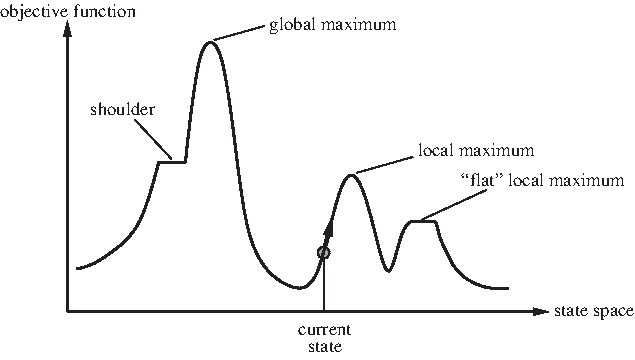
\includegraphics[width=0.75\textwidth]{img/topologia-espaco-busca}
	\caption{Uma representação da topologia de um espaço de estados unidimensional}
	\label{fig:topologia-espaco-busca}
\end{figure}

Considerando este espaço de busca para um problema de maximização, queremos encontrar a solução com maior valor possível para a função objetivo. Esta solução é chamada de máximo global e está representada na Figura~\ref{fig:topologia-espaco-busca}. O máximo global, além de ser o estado (ou a solução) que possui maior valor para a função objetivo, tem a característica de que todos os seus vizinhos possuem valor de função objetivo menores ou iguais ao seu. Portanto, se a busca encontrar uma solução com esta segunda característica, sabemos que trata-se de um máximo, mas não podemos garantir que este seja o máximo global, pois pode ocorrer em outras regiões do espaço de busca e não possuir o maior valor para a função objetivo. Neste caso, trata-se de um máximo local, também representado na Figura~\ref{fig:topologia-espaco-busca}. Finalmente, existem regiões em que as todas as soluções vizinhas possuem o mesmo valor de função objetivo. Este caso é chamado de platô (ou \textit{plateau}), ou ainda planície (representado pela região \textit{shoulder} na Figura~\ref{fig:topologia-espaco-busca}).

Conhecer as possíveis situações que a busca vai encontrar em diferentes topologias é importante para entender as limitações de uma busca local e os casos específicos com os quais se preocupar. Como a busca local somente seleciona vizinhos que melhoram a função objetivo, caso ela encontre um máximo local, não conseguirá ``sair'' desta solução. Observe o estado atual representado na Figura~\ref{fig:topologia-espaco-busca}. Esta solução encontra-se subindo na sua vizinhança, pois a busca tenta sempre melhorá-la. Ao chegar no máximo local, nenhum vizinho possui um melhor (maior) valor de função objetivo e a busca termina. No entanto, esta não é a melhor solução para o problema. A mesma situação acontece em platôs, onde uma busca local simples não é capaz de superá-los.

Portanto, uma busca local simples, do tipo subida da encosta, tem como critério de parada o fato de encontrar uma solução ótima, que não é garantidamente o ótimo global do problema. Esta é a deficiência desta busca e diferentes estratégias são adotadas para superá-la, dando origem às variantes da busca local.

\subsection{Exemplo: problema das 8 rainhas}

Consideremos o problema das 8-rainhas. É sabido que duas rainhas não podem estar na mesma linha ou coluna. Portanto, uma boa estratégia consiste em distribuir inicialmente cada rainha em uma das colunas e em linhas aleatórias gerando, assim, a solução inicial. Cada rainha permanece na sua coluna, portanto o movimento consiste em selecionar uma rainha e movê-la para outro quadrado da mesma coluna. Cada estado possui $8 \times 7 = 56$ estados sucessores, que compõem sua vizinhança. A função objetivo pode ser definida como o número de pares de rainhas que estão se atacando. O mínimo global dessa função é zero, que só ocorre em soluções perfeitas.

A Figura~\ref{fig:busca-local-oito-rainhas} mostra um possível estado para o problema, cuja função objetivo possui valor $17$. No tabuleiro, são apresentados os valores da função objetivo das soluções vizinhas. Percebe-se que alguns movimentos diminuem a função objetivo para $12$, que é a melhor melhora possível. Uma busca local, portanto, seleciona vizinhos que melhoram o valor da função objetivo de acordo com alguma das estratégias apresentadas.

\begin{figure}[h]
	\centering
	\hspace{15pt}
	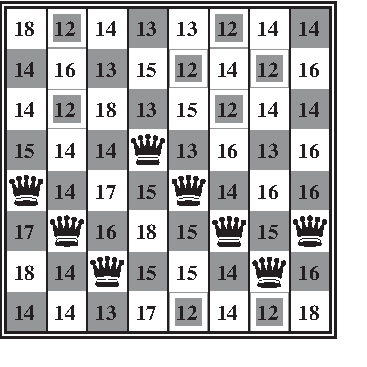
\includegraphics[width=0.5\textwidth]{img/busca-local-oito-rainhas}
	\caption{Uma solução parcial com custos para o problema das 8 rainhas}
	\label{fig:busca-local-oito-rainhas}
\end{figure}

Conforme discutido nas seções anteriores, a deficiência da busca local simples (subida da montanha) é a incapacidade de superar ótimos locais. O espaço de busca do problema das 8 rainhas é caracterizado por muitos mínimos locais, o que dificulta o desempenho da busca local. A Figura~\ref{fig:minimo-local-oito-rainhas} apresenta um mínimo local para o problema das 8 rainhas, cuja função objetivo soma $1$ (muito próximo da solução), mas todos os vizinhos possuem valores maiores.

\begin{figure}[h]
	\centering
	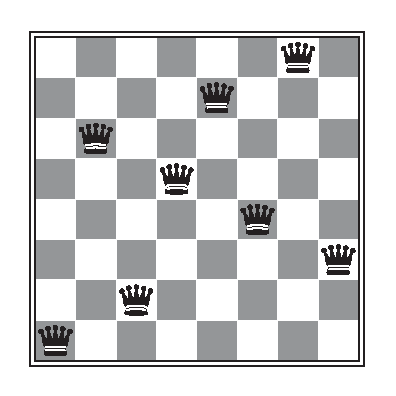
\includegraphics[width=0.55\textwidth]{img/minimo-local-oito-rainhas}
	\caption{Um mínimo local para o problema das 8 rainhas}
	\label{fig:minimo-local-oito-rainhas}
\end{figure}

Devido à topologia do seu espaço de estados, uma busca local retorna um ótimo local em aproximadamente 86\% dos casos para o problema das 8 rainhas e, portanto, resolve em apenas 14\% das vezes. Apesar disso, a convergência é rápida, pois a busca demora cerca de quatro passos quando encontra a solução ótima, e três passos quando encontra um ótimo local. Isso mostra o potencial da busca local, pois o espaço de busca contém $8^8 \approx 17$ milhões de estados.

Para chegar à solução ótima, o algoritmo deve adotar alguma estratégia para superar ótimos locais. Por exemplo, a busca poderia permitir soluções piores, visando uma melhora futura. As próximas seções apresentam variantes da busca local com o objetivo de superar esta deficiência.

\subsection{Busca local randomizada}

Uma primeira estratégia para superar ótimos locais consiste em incluir um componente aleatório que permite selecionar vizinhos iguais ou piores. Neste sentido, a busca local randomizada (ou \textbf{busca local estocástica}) recebe um parâmetro $p \in [0,1]$ como entrada, que define a probabilidade da busca fazer um movimento aleatório. Com probabilidade $p$ a busca seleciona um vizinho qualquer, e com probabilidade $1 - p$ a busca escolhe um vizinho melhor de acordo com alguma sub-estratégia de seleção (primeira melhora, melhor melhora ou melhora aleatória).

\begin{algorithm}[h]
	\DontPrintSemicolon
	\Entrada{\textit{solução inicial} -- $s$, \textit{probabilidade} -- $p$}
	\Saida{\textit{melhor solução encontrada} -- $s^*$}
	
	\Inicio{
		$s^* \gets s$\;
		\Enqto{critério de parada não satisfeito}{
			num $\gets$ randomFloat() \textit{//de 0 a 1}\;
			\Se{num $\le p$}{
				seleciona qualquer vizinho $s' \in N(s)$\;
			}
			\Senao{
				seleciona vizinho melhor $s' \in N(s)$\;
			}
			
			$s \gets s'$\;
			\Se{$\varphi(s) < \varphi(s^*)$}{
				$s* \gets s$\;
			}
		}
		\Retorna{$s^*$}
	}
	
	\caption{Pseudocódigo para uma busca local randomizada}
	\label{alg:busca-local-randomizada}
\end{algorithm}

O Algoritmo~\ref{alg:busca-local-randomizada} apresenta o pseudocódigo para uma busca local randomizada. A estratégia de randomização é implementada nas linhas 4 a 8, que seleciona os vizinhos em função da probabilidade $p$. Apesar de simples, esta estratégia consegue superar ótimos locais. No entanto, exigindo a calibração de $p$\footnote{Perceba que assumindo $p = 0$, temos uma busca local simples, enquanto com $p = 1$ temos uma \textbf{caminhada aleatória} no espaço de busca.}. O critério de parada pode ser a qualidade da melhor solução conhecida, o número de iterações sem melhora, o número máximo de iterações ou um limite em tempo de execução.

\subsection{Busca local iterada}

Uma segunda abordagem consiste em reiniciar a busca sempre que ela encontra um ótimo local. Isto é, executar a busca local repetidamente de forma a, em uma das execuções, encontrar o ótimo global. Uma alternativa mais interessante consiste em executar uma busca local iterativamente, alterando parte da solução sempre que um ótimo local for encontrado. Esta alteração é chamada de \textbf{perturbação} e o algoritmo é chamado de busca local iterada (\textbf{iterated local search}). Seu funcionamento é expresso no Algoritmo~\ref{alg:busca-local-iterada}.

\begin{algorithm}[h]
	\DontPrintSemicolon
	\Entrada{\textit{solução inicial} -- $s$}
	\Saida{\textit{melhor solução encontrada} -- $s^*$}
	
	\Inicio{
		$s^* \gets s$\;
		\Enqto{critério de parada não satisfeito}{
			s $\gets$ perturba($s$)\;
			s $\gets$ buscaLocal($s$)\;
			\Se{$\varphi(s) < \varphi(s^*)$}{
				$s* \gets s$\;
			}
		}
		\Retorna{$s^*$}
	}
	
	\caption{Pseudocódigo para uma busca local iterada}
	\label{alg:busca-local-iterada}
\end{algorithm}

Em resumo, uma busca local iterada repetidamente perturba uma solução e aplica uma busca local, armazenando a melhor solução encontrada. A perturbação consiste em modificar a solução de forma que na próxima busca local, outro ótimo seja encontrado. Um parâmetro que pode ser incluído na busca é o tamanho da perturbação, isto é, quanto da solução será modificada. No problema das 8 rainhas, por exemplo, uma possível perturbação consiste em selecionar parte das rainhas e mover para uma posição aleatória da mesma coluna. O critério de parada pode ser a qualidade da melhor solução conhecida, o número de iterações sem melhora, o número máximo de iterações ou um limite em tempo de execução.

\subsection{Simulated annealing}

As estratégias de busca local randomizada e busca local iterada tornam a busca completa, mas podem se apresentar ineficientes de acordo com o tamanho e topologia do espaço de busca. O algoritmo de simulated annealing (ou \textbf{têmpera simulada}) é uma tentativa de obter completude de forma mais eficiente. Esta abordagem foi proposta por \citet{KirkpatrickEtAl1983} e \citet{Cerny1985} e faz uma analogia à evolução de um sólido para o equilíbrio térmico, no processo conhecido como têmpera ou arrefecimento de metais. A ideia básica consiste em explorar o espaço de busca, aceitando soluções piores com maior probabilidade no início e decrescendo esta probabilidade com o passar do tempo, similar à diminuição de temperatura de uma têmpera.

O simulated annealing utiliza o \textbf{critério de aceitação de Metropolis}~\citep{MetropolisEtAl1953}, dado por:
$$
P[\text{aceitar } s' \mid s] = 
\begin{cases}
	1  & \text{caso } s' \text{ seja melhor que } s \\
	e^{-\Delta(s, s')/T}  & \text{caso contrário.}
\end{cases}
$$
Caso a nova solução $s'$ seja melhor, ela é sempre aceita. Caso ela seja pior, a probabilidade de ela ser aceita varia em função do quanto ela piora a solução atual $\Delta(s, s') = \varphi(s') - \varphi(s)$ e da temperatura $T$. A temperatura evolui, diminuindo a cada iteração. Dessa forma, no início a busca aceita mais soluções piores, enquanto no final a busca é intensificada (para soluções de melhor qualidade).

\begin{algorithm}[h]
	\DontPrintSemicolon
	\Entrada{\textit{solução inicial} -- $s$, \textit{temperatura inicial} -- $T_0$, \textit{temperatura final} -- $T_{final}$}
	\Saida{\textit{melhor solução encontrada} -- $s^*$}
	
	\Inicio{
		$s^* \gets s$\;
		$T \gets T_0$
		
		\Enqto{$T > T_{final}$}{
			seleciona vizinho $s' \in N(s)$ aleatoriamente\;
			\Se{$\Delta(s, s') <= 0$}{
				$s \gets s'$\;
			}
			\Senao{
				$s \gets s'$ com probabilidade $e^{-\Delta(s, s')/T}$\;
			}
			
			\Se{$\varphi(s) < \varphi(s^*)$}{
				$s* \gets s$\;
			}
			
			$T \gets$ proximaTemperatura($T$)\;
		}
		\Retorna{$s^*$}
	}
	
	\caption{Pseudocódigo para o algoritmo de simulated annealing}
	\label{alg:simulated-annealing}
\end{algorithm}

O Algoritmo~\ref{alg:simulated-annealing} apresenta o pseudocódigo do simulated annealing. Os parâmetros $T$, $T_{final}$ e a definição da estratégia de atualização de temperatura (linha 12) devem ser ajustados empiricamente, pois sua performance varia em função do problema. \citet{RusselAndNorvig2010} explicam didaticamente o método de simulated annealing da seguinte forma:

\begin{quotation}
``\textit{Para explicar a têmpera simulada, vamos mudar nosso ponto de vista de subida de encosta para descida de gradiente (isto é, minimização do custo) e imaginar a tarefa de colocar uma bola de pingue-pongue na fenda mais profunda em uma superfície acidentada. Se simplesmente deixarmos a bola rolar, ela acabará em um mínimo local. Se agitarmos a superfície, poderemos fazer a bola quicar para fora do mínimo local. O artifício é agitar com força suficiente para fazer a bola sair dos mínimos locais, mas não o bastante para desalojá-la do mínimo global. A solução de têmpera simulada é começar a agitar com força (isto é, em alta temperatura) e depois reduzir gradualmente a intensidade da agitação (ou seja, baixar a temperatura).}''
\end{quotation}

\section{Algoritmos genéticos}

Os algoritmos genéticos fazem parte de uma área de estudos chamada \textbf{computação evolucionária} (veja mais detalhes em \citet{EibenAndSmith2003}) e são uma metaheurística baseada em recombinação de soluções. Suas ideias se baseiam na teoria da evolução de Darwin e no mecanismo de seleção natural que fazem com que as espécies evoluam. Dessa forma, os algoritmos genéticos propõem a evolução de soluções mediante o processo de seleção natural. Por conta disso, esta abordagem compõe, juntamente com outras áreas da computação e da inteligência artificial, uma vertente chamada computação bioinspirada, ou computação baseada na natureza.

Em resumo, os seres vivos competem entre si por recursos limitados. Nesta competição, apenas os indivíduos mais aptos sobrevivem (seleção natural). Os seres vivos se reproduzem, gerando descendentes que herdam as características dos pais. Logo, as características de aptidão são passadas para as próximas gerações. Esta seção apresenta a forma como estes conceitos são aplicados aos algoritmos genéticos para a solução de problemas de otimização.

\subsection{Esquema geral}

Podemos decompor um algoritmo genético nas etapas ilustradas na Figura~\ref{fig:algoritmo-genetico}. Cada etapa é apresentada como um bloco, juntamente com o fluxo de execução entre elas. A população é composta por soluções viáveis do problema, isto é, estados possíveis para o problema. Na primeira etapa esta população é inicializada, ou seja, são criadas várias soluções, conforme o tamanho desejado para a população. Para cada indivíduo, é calculada sua aptidão (segunda etapa), que consiste na qualidade da solução. Caso algum critério de terminação seja satisfeito, a busca termina. Como critérios de terminação pode-se definir um número máximo de iterações, tempo limite, qualidade mínima da melhor solução encontrada, número máximo de iterações sem aumento significativo da aptidão máxima da população, entre outras.

\begin{figure}[H]
	\centering
	
	\tikzstyle{decision} = [diamond, draw, fill=blue!20, text width=6em, text badly centered, node distance=3cm, inner sep=0pt]
	\tikzstyle{block} = [rectangle, draw, fill=blue!20, text width=6.4em, text centered, rounded corners, minimum height=4em]
	\tikzstyle{line} = [draw, -latex']
	\tikzstyle{cloud} = [draw, ellipse,fill=red!20, node distance=3cm, minimum height=2em]	
	
	\begin{tikzpicture}[node distance = 2.5cm, auto]
		\node [block] (inicializa) {Inicializa população};
		\node [block, below of=inicializa] (aptidao) {Calcula aptidão};
		\node [decision, below of=aptidao, node distance=3.5cm] (terminacao) {Critério terminação?};
		\node [block, below of=terminacao, node distance=3.5cm] (selecao) {Seleção};
		\node [block, below of=selecao] (recombinacao) {Recombinação};
		\node [block, below of=recombinacao] (mutacao) {Mutação};
		\node [block, below of=mutacao] (substitui) {Substitui população};
		\node [left of=selecao, node distance=4cm] (temp) {Nova geração};
		\node [block, right of=terminacao, node distance=4.5cm] (fim) {Fim};
		
		\path [line] (inicializa) -- (aptidao);
		\path [line] (aptidao) -- (terminacao);
		\path [line] (terminacao) -- node {não}(selecao);
		\path [line] (selecao) -- (recombinacao);
		\path [line] (recombinacao) -- (mutacao);
		\path [line] (mutacao) -- (substitui);
		\draw (substitui) -| (temp);
		\path [line] (temp) |- (aptidao);
		\path [line] (terminacao) -- node {sim}(fim);
	\end{tikzpicture}
	
	\caption{Esquema geral de um algoritmo genético}
	\label{fig:algoritmo-genetico}
\end{figure}

Enquanto a busca não termina, parte da população é selecionada para a recombinação (terceira etapa). O número de indivíduos selecionados pode ser uma quantidade fixa ou um percentual do tamanho da população. A escolha de quais indivíduos serão selecionados é realizada em função do valor de aptidão de cada um (ex: indivíduos mais aptos recombinam). Cada par\footnote{Um número diferente de indivíduos pode ser utilizado na recombinação. Ex: três indivíduos recombinam e geram dois filhos.} de indivíduos selecionados é recombinado (quarta etapa), gerando novos indivíduos.

Os indivíduos que fazem parte da população e os indivíduos gerados podem sofrer uma mutação, que consiste na alteração de parte da solução. A mutação é utilizada como fator de diversificação da busca, similar à perturbação utilizada na busca local iterada. Finalmente, são selecionados os indivíduos (da população original e dos novos) para comporem a nova população. Esta seleção é geralmente realizada em função da aptidão dos indivíduos (os mais aptos, mais um pequeno grupo de menos aptos para diversificação). Este mesmo esquema geral está expresso no Algoritmo~\ref{alg:algoritmo-genetico}.

\begin{algorithm}[h]
	\DontPrintSemicolon
	\Entrada{\textit{parâmetros das etapas}}
	\Saida{\textit{melhor solução encontrada}}
	
	\Inicio{
		populacao $\gets$ inicializaPopulacao()\;
		calculaAptidao(populacao)\;
		
		\Se{critério de terminação satisfeito}{
			\Retorna{melhor solução da população}	
		}
		
		popRecombinar $\gets$ selecao(populacao)\;
		novosIndividuos $\gets$ recombinacao(popRecombinar)\;
		mutacao(populacao $\cup$ novosIndividuos)\;
		populacao $\gets$ substitui(populacao $\cup$ novosIndividuos)\;
	}
	
	\caption{Pseudocódigo para um algoritmo genético}
	\label{alg:algoritmo-genetico}
\end{algorithm}

As próximas seções apresentam os componentes que precisam ser projetados para o desenvolvimento de um algoritmo genético, bem como detalham as etapas discutidas nesta seção.

\subsection{Representação de estados/soluções}

Para exemplificar os passos na construção de um algoritmo genético, vamos considerar um problema simples de maximizar a função $f(x) = x^2$, com o domínio de $x \in [0, 63]$. Chamaremos este problema de ``maximização de função quadrática'' e podemos formalizá-lo como
$$
\begin{aligned}
	& \text{maximiza} & & f(x) = x^2 \\
	& \text{sujeito a} & & x \in [0, 63].
\end{aligned}
$$

Uma vez definido o problema a ser tratado, o primeiro passo consiste em determinar uma \textbf{representação cromossomial} (ou representação na forma de cromossomo) para a solução (estado). Consiste em uma representação \textbf{sequencial}, que permita realizar as operações de cálculo de aptidão, cruzamento (recombinação) e mutação. Para o problema da maximização de função quadrática, temos 64 soluções diferentes, que são números inteiros de 0 a 63. Uma representação cromossomial comum é a representação binária, que pode ser utilizada para representar o domínio em questão. Sendo assim, precisamos de 6 bits para representar o intervalo desejado. Por exemplo, o número 0 é representado por \texttt{000000}, o número 11 é representado por \texttt{001011}, o número 46 é representado por \texttt{101110} e o número 63 é representado por \texttt{111111}. A solução original (representação decimal) é chamada de \textbf{fenótipo}, sua representação sequencial é chamada de \textbf{cromossomo} e cada posição desta sequência é chamado de \textbf{gene}. Logo, cada valor binário dos exemplos anteriores é um gene do cromossomo, que é composto por 6 genes.

Apesar da maioria dos algoritmos genéticos utilizar uma representação binária, isso não é uma regra. É possível definir outras formas de representação sequencial. O problema das 8 rainhas, por exemplo, pode ser representado por um vetor de inteiros de 8 posições. Cada posição $i$ armazena valores de $1$ a $8$, que representam o quadrado que a rainha $i$ ocupa na coluna $i$.

Além da representação da solução, é preciso definir a função objetivo, que calcula a qualidade da solução. No contexto dos algoritmos genéticos, a função objetivo é chamada de \textbf{função de fitness} e a qualidade da solução é chamada de \textbf{fitness} ou \textbf{aptidão}. No caso do problema de maximização de função quadrática, a função de fitness é a própria função $f(x) = x^2$. Por exemplo, a solução $0 =$ \texttt{000000} possui fitness de $0$. A solução $11 =$ \texttt{001011} possui fitness de $121$. A solução $46 =$ \texttt{101110} possui fitness de 2116. A solução $63 =$ \texttt{111111} possui fitness de 3969 e, obviamente, é a solução ótima.

\textbf{Observação:} perceba que em um problema de minimização, quanto menor o valor da função objetivo, maior a qualidade da solução. Neste caso, a função de fitness pode ser definida como a inversa da função objetivo ($1/\varphi(s)$). Caso contrário, as demais etapas devem ser ajustadas para tratar uma função de fitness de minimização.

\subsection{Seleção de indivíduos}

A etapa de seleção define quais indivíduos serão utilizados para a recombinação. A estratégia mais simples consiste em selecionar todos os indivíduos. No entanto, esta abordagem pode ser ineficiente, pois o tempo de processamento é alto. Outra abordagem consiste em selecionar apenas parte da população. Selecionar apenas os indivíduos com maior aptidão não é adequado, pois pode enviesar a busca. O ideal é selecionar os bons indivíduos e alguns com menor aptidão para diversidade.

Uma abordagem simples consiste em selecionar os 50\% melhores indivíduos, juntamente com os 10\% piores (estes percentuais podem ser ajustados). Uma segunda abordagem seleciona indivíduos probabilisticamente. Quanto maior a aptidão do indivíduo, maior a probabilidade de ser selecionado. Uma proposta amplamente utilizada é
$$
P[\text{selecionar } i] = \frac{fitness(i)}{\sum_{j} fitness(j)}
$$

\begin{table}[h]
	\centering
	
	\begin{tabular}{L{3cm}R{2.5cm}R{2.5cm}R{4.5cm}}
		\hline
		\textbf{Cromossomo} & \textbf{Fenótipo} & \textbf{Fitness} & $P[\text{selecionar }i]$ \\
		\hline
		\texttt{000000} & 0 & 0 & 0 \\
		\texttt{001011} & 11 & 121 & $121/6206 = 0,02$ \\
		\texttt{101110} & 46 & 2116 & $2116/6206 = 0,34$ \\
		\texttt{111111} & 63 & 3969 & $3969/6206 = 0,64$ \\
		\hline
	\end{tabular}
	
	\caption{Exemplo de seleção probabilística para a maximização de função quadrática}
	\label{tab:selecao-probabilistica}
\end{table}

\insertspace

A Tabela~\ref{tab:selecao-probabilistica} mostra quatro soluções para o problema de maximização de função quadrática, com o respectivo fitness e a probabilidade de seleção de recombinação. O somatório dos valores de fitness é 6206. Perceba que qualquer solução (exceto com fitness 0) pode ser selecionada. A seleção apenas prioriza soluções com maior aptidão.

Uma abordagem para a implementação de decisões probabilísticas é chamado de \textbf{método da roleta}. Consiste em definir o intervalo de valores para seleção dos indivíduos. A Tabela~\ref{tab:selecao-probabilistica-roleta} mostra a probabilidade acumulada de cada indivíduo, isto é, a sua probabilidade somada às probabilidades dos indivíduos anteriores. Com isso, ao sortear um número, verificamos em qual intervalo ele se encontra e selecionamos o indivíduo correspondente. Por exemplo, se sorteamos o número 0,12, percebemos que se encontra entre 0,02 e 0,36. Logo, selecionamos o indivíduo \texttt{101110}. Ao sortear o número 0,7, percebemos que se encontra entre 0,36 e 1,0. Logo, selecionamos o indivíduo \texttt{111111}.

\begin{table}[h]
	\centering
	
	\begin{tabular}{L{3cm}R{2cm}R{2cm}R{3cm}R{2.5cm}}
		\hline
		\textbf{Cromossomo} & \textbf{Fenótipo} & \textbf{Fitness} & $P[\text{selecionar }i]$ & \textbf{Acumulado}\\
		\hline
		\texttt{000000} & 0 & 0 & 0 & 0 \\
		\texttt{001011} & 11 & 121 & $0,02$ & $0,02$ \\
		\texttt{101110} & 46 & 2116 & $0,34$ & $0,36$ \\
		\texttt{111111} & 63 & 3969 & $0,64$ & $1,0$ \\
		\hline
	\end{tabular}
	
	\caption{Exemplo de seleção probabilística pelo método da roleta}
	\label{tab:selecao-probabilistica-roleta}
\end{table}

\subsection{Recombinação de indivíduos}

A etapa de recombinação utiliza os indivíduos selecionados para gerar novos indivíduos. Ela pode ser vista como a reprodução dos indivíduos dessa população. A forma mais comum de recombinação é o \textbf{cruzamento} realizado entre um par de indivíduos. No entanto, existem outros operadores de recombinação, assim como a recombinação pode ser realizada com um número maior de indivíduos. Este material apresenta três formas de cruzamento, que é realizado com um par de indivíduos e gera dois descendentes (filhos).

O \textbf{cruzamento de ponto único} define um ponto de corte para dividir o cromossomo de cada solução pai. Os novos cromossomos são gerados combinando as metades de cada pai.

\insertspace
\textbf{Exemplo}
\begin{align*}
	\textbf{Soluções pai:}	& \hspace{1cm} \textbf{{\color{blue}101}|{\color{blue}001}} \\
							& \hspace{1cm} \textbf{{\color{red}011}|{\color{red}100}}
\end{align*}
\begin{center}
	\makebox[7cm]{\hrulefill}
\end{center}
\begin{align*}
	\textbf{Descendentes:}	& \hspace{1cm} \textbf{{\color{blue}101}|{\color{red}100}} \\
							& \hspace{1cm} \textbf{{\color{red}011}|{\color{blue}001}}
\end{align*}

O \textbf{cruzamento com dois pontos} segue a mesma ideia de cruzamento, porém utilizando dois pontos de corte. Observe que neste caso é possível gerar mais de dois descendentes, uma vez que o número de combinações possíveis das partes é maior.

\insertspace
\textbf{Exemplo}
\begin{align*}
	\textbf{Soluções pai:}	& \hspace{1cm} \textbf{{\color{blue}10}|{\color{blue}10}|{\color{blue}01}} \\
							& \hspace{1cm} \textbf{{\color{red}01}|{\color{red}11}|{\color{red}00}}
\end{align*}
\begin{center}
	\makebox[7cm]{\hrulefill}
\end{center}
\begin{align*}
	\textbf{Descendentes:}	& \hspace{1cm} \textbf{{\color{blue}10}|{\color{red}11}|{\color{blue}01}} \\
							& \hspace{1cm} \textbf{{\color{red}01}|{\color{blue}10}|{\color{red}00}}
\end{align*}

O \textbf{cruzamento uniforme} seleciona genes de ambos os pais conforme uma distribuição predefinida, dada por um padrão. Comumente, cada posição deste padrão é gerado aleatoriamente, com igual probabilidade de selecionar o valor de cada pai, por isso o nome de cruzamento uniforme. Por exemplo, o padrão \texttt{ABAABA} seleciona os genes 1, 3, 4 e 6 do primeiro indivíduo (\texttt{A}), e seleciona os genes 2 e 5 do segundo indivíduo (\texttt{B}). Isto é suficiente para gerar um descendente. No caso da geração de dois descendentes, o segundo seleciona os genes de forma inversa~\footnote{Uma outra possibilidade consiste em estimar a contribuição de cada gene das soluções na aptidão da mesma e selecionar segundo este valor.}.

\insertspace
\textbf{Exemplo}

\begin{center}
	\textbf{Padrão:} \texttt{AABABB}
\end{center}
\begin{center}
	\makebox[7cm]{\hrulefill}
\end{center}
\begin{align*}
	\textbf{Soluções pai:}	& \hspace{1cm} \textbf{\color{blue}101001} \\
	& \hspace{1cm} \textbf{\color{red}011100}
\end{align*}
\begin{center}
	\makebox[7cm]{\hrulefill}
\end{center}
\begin{align*}
	\textbf{Descendentes:}	& \hspace{1cm} \textbf{{\color{blue}10}{\color{red}1}{\color{blue}0}{\color{red}00}} \\
	& \hspace{1cm} \textbf{{\color{red}01}{\color{blue}1}{\color{red}1}{\color{blue}01}}
\end{align*}

\subsection{Mutação de indivíduos}

Conforme apresentado, a mutação é um componente de diversificação da busca. Consiste em modificar parte da solução, como a alteração no valor de um ou mais genes. Neste sentido, o algoritmo genético possui dois parâmetros: taxa de mutação e tamanho da mutação. A taxa de mutação $m \in [0, 1]$ define a probabilidade do indivíduo sofrer mutação. O tamanho da mutação $t_m$ define quantos genes serão modificados. Em geral, assume-se $t_m = 1$.

Com a população completa (população inicial e indivíduos gerados na recombinação), cada indivíduo pode sofrer mutação com probabilidade $m$, isto é, $P[\text{mutar } i] = m, \forall i$. No caso de uma representação binária, a mutação consiste em trocar o valor de $t_m$ genes aleatórios.

A implementação dessa estratégia probabilística segue a mesma ideia da roleta. Se o número sorteado (no intervalo 0 a 1) for menor ou igual que a taxa de mutação $m$, o indivíduo sofre mutação. Por exemplo, considerando $m = 0,05$ (5\% de chance do indivíduo sofrer mutação), ao sortear o número $0,35$, o indivíduo não sofre mutação. Em contrapartida, ao sortear o número $0,043$, o indivíduo sofre mutação.

\subsection{Substituição da população}

Após as fases anteriores, existem indivíduos da população anterior e indivíduos gerados na recombinação. De todos estes indivíduos, devem ser selecionados aqueles que farão parte da população da próxima iteração. Existem diversas estratégias de substituição da população. A \textbf{estratégia elitista} consiste em selecionar os melhores indivíduos e, possivelmente, indivíduos com menor aptidão. A seleção de indivíduos ``ruins'' é importante como mecanismo de diversificação, evitando uma busca enviesada.

Outras abordagens propõem que a nova população seja selecionada apenas dos novos indivíduos. Ou ainda, que a população deve ser renovada de tempos em tempos, após um determinado número de iterações. Cada nova população é chamada de \textbf{geração} e, portanto, uma iteração do algoritmo genético é também chamado de geração.

\section{Recursos disponíveis}

Algumas ferramentas, conhecidas como solvers, implementam algoritmos heurísticos para a solução de problemas de otimização combinatória. O site Spreadsheet Analytics~\footnote{\url{https://sites.google.com/a/usfca.edu/business-analytics/model-driven-analytics/solvers/meta-heuristics}} apresenta algumas delas. Estas ferramentas podem ser usadas para uma análise inicial da solução de problemas dessa natureza através de metaheurísticas. Uma ferramenta de destaque é o HeuristicLab~\footnote{\url{https://dev.heuristiclab.com}}, que implementa uma variedade de metaheurísticas, como buscas locais, métodos construtivos e populacionais, e ainda fornece uma interface gráfica para o uso e apresentação dos resultados. Uma segunda ferramenta black-box é o LocalSolver~\footnote{\url{http://www.localsolver.com}}, que fornece uma linguagem de modelagem para a aplicação em qualquer problema de otimização. Para programação matemática e métodos exatos, a Google disponibiliza o Google Optimization Tools~\footnote{\url{https://developers.google.com/optimization}}.

Além das ferramentas, existem diversas bibliotecas que podem ser utilizadas no desenvolvimento de metaheurísticas. \cite{FinkEtAl2003} discute algumas delas, comentando sobre os métodos heurísticos implementados. Para a linguagem Java, duas opções são a BiCIAM~\footnote{\url{http://modo.ugr.es/algorithmportfolio}} e a JAMES~\footnote{\url{http://www.jamesframework.org/}}. Para MATLAB se destaca a MHTB~\footnote{\url{http://neo.lcc.uma.es/software/mhtb}}.

\section{Exercícios}
\resetexercisenumbering

\begin{exercise}
Explique por que uma busca local do tipo subida da encosta frequentemente retorna um ótimo local. Ilustre a explanação através de um exemplo.
\end{exercise}

\begin{exercise}
Considere o problema de maximização da função $f(x) = x^2 - 4x$, formalizado como
$$
\begin{aligned}
	& \text{maximiza} & & f(x) = x^2 - 4x \\
	& \text{sujeito a} & & x \in [0, 10].
\end{aligned}
$$

A solução é composta por um número inteiro no intervalo de 0 a 10 e a vizinhança é composta pelo incremento e decremento do valor em 1. Por exemplo, a solução `6' possui como vizinhança as soluções `5' e `7'. O que acontece se executarmos uma busca local do tipo subida da encosta com solução inicial igual a `1'? E se executarmos a mesma busca com solução inicial igual a `3'? Finalmente, o que acontece se executarmos a busca com solução inicial igual a `2'?

\textbf{Dica:} plote o gráfico da função objetivo para visualizar o espaço de busca.

\end{exercise}

\begin{exercise}
O problema do \textbf{caixeiro viajante} (PCV) consiste em encontrar o menor caminho em um mapa, saindo de uma cidade, visitando todas as cidades uma única vez e retornando à cidade de origem. Em outras palavras, dado um grafo completo, encontrar o menor ciclo hamiltoniano. Considere a instância abaixo composta por 5 cidades \texttt{(a)}, cujas distâncias são dadas pela matriz de adjacências \texttt{(b)}.

\begin{figure}[h]
	\centering

\subfigure[]{
	\begin{tikzpicture}
		\draw
			(0, 0) node[circle, draw] (a) {A}
			(-2, -1.25) node[circle, draw] (b) {B}
			(-1, -3) node[circle, draw] (c) {C}
			(1, -3) node[circle, draw] (d) {D}
			(2, -1.25) node[circle, draw] (e) {E};
			
		\draw (a) -- (b);	
		\draw (a) -- (d);
		\draw (a) -- (c);
		\draw (a) -- (e);
		\draw (b) -- (d);
		\draw (b) -- (e);
		\draw (b) -- (c);
		\draw (c) -- (d);
		\draw (c) -- (e);
		\draw (d) -- (e);
	\end{tikzpicture}
}
\subtable[]{
	\begin{tabular}[b]{c|ccccc}
		& \textbf{A} & \textbf{B} & \textbf{C} & \textbf{D} & \textbf{E} \\
		\hline
		\textbf{A} & 0 & 10 & 5 & 3 & 12 \\
		\textbf{B} & 10 & 0 & 6 & 8 & 10 \\
		\textbf{C} & 5 & 6 & 0 & 9 & 1 \\
		\textbf{D} & 3 & 8 & 9 & 0 & 4 \\
		\textbf{E} & 12 & 10 & 1 & 4 & 0 \\
	\end{tabular}
}
\end{figure}

\end{exercise}

Uma solução é representada pela lista ordenada de cidades. Por exemplo, um caminho que inicie na cidade \texttt{A}, siga para as cidades \texttt{B}, \texttt{C}, \texttt{D}, \texttt{E} e retorne para a cidade \texttt{A} é representada por \{A,B,C,D,E\}. Esta solução possui um custo total de 41, que é o somatório dos custos dos caminhos entre as cidades, conforme matriz de adjacências.

Mostre a execução de uma busca local simples, considerando que a vizinhança é composta pela permutação de duas posições vizinhas na solução. A seleção do vizinho utiliza a estratégia \textit{melhor melhora}. Considere como solução inicial o caminho \{A, E, B, D, C\}. Qual a solução resultante dessa busca? Trata-se de um mínimo local ou global?

Mostre a execução de uma busca local randomizada com $p = 0,2$. Cada vez que necessitar de uma decisão aleatória, considere o sorteio do próximo número da sequência abaixo. Quantas iterações a busca precisa para encontrar o ótimo global? A busca melhora se alterarmos o valor de $p$?

\begin{itemize}
	\item 0,4; 0,12; 0,08; 0,93; 0,71; 0,44; 0,1; 0,67; 0,83; 0,21; 0,09; 0;13; 0,7.
\end{itemize}

\insertspace

\begin{exercise}
Considere o problema das $N$-Rainhas com $N = 5$ (podemos chamar de problema das 5-Rainhas). O tabuleiro possui tamanho $5 \times 5$. Uma solução é representada por um vetor de inteiros $x = (r_1, r_2, r_3, r_4, r_5)$, onde $r_i$ representa a linha que a rainha $r$ ocupa na coluna $i$. A função objetivo corresponde ao número pares de rainhas que se atacam. Mostre a execução de um algoritmo genético considerando os parâmetros abaixo:
\begin{itemize}
	\item \textbf{Tamanho da população:} 5.
	\item \textbf{Função de fitness:} $1/$função objetivo.
	\item \textbf{Critério de parada:} solução encontrada (função objetivo igual a zero).
	\item \textbf{Estratégia de seleção para recombinação:} 3 melhores indivíduos.
	\item \textbf{Recombinação:} cruzamento com um ponto de corte entre $r_2$ e $r_3$.
	\item \textbf{Mutação:} troca o valor aleatoriamente de uma posição, também aleatória, da solução. O indivíduo sofre mutação com probabilidade $0.1$.
	\item \textbf{Substituição da população:} toda a população anterior é substituída pela nova população, exceto o melhor indivíduo.
\end{itemize}

\insertspace

Considere a seguinte população inicial:
\begin{itemize}
	\item $x_1 = (1, 3, 2, 4, 5)$
	\item $x_2 = (2, 3, 4, 1, 5)$
	\item $x_3 = (1, 4, 5, 2, 3)$
	\item $x_4 = (3, 4, 5, 1, 3)$
	\item $x_5 = (5, 5, 2, 3, 1)$
\end{itemize}

\insertspace

Para as decisões probabilísticas, considere a seguinte sequência de números sorteados:
\begin{itemize}
	\item 0,1; 0,4; 0,3; 0,02; 0,9; 0,05; 0,65; 0,43; 0,7; 0,1; 0,18; 0,2; 0,6; 0,85; 0,7; 0,08; 0,89.
\end{itemize}

\insertspace

Para facilitar o cáclulo do custo das soluções, pode-se utilizar o programa abaixo.

\begin{minted}{java}
public class CustoNRainhas {
	public static void main(String[] args) {
		int n = 5;
		int[] x = {5, 2, 1, 3, 4};
		int custo = 0;
		
		for(int i = 0; i < n; i++) {
			for(int j = 0; j < n; j++) {
				if(i == j) break;
				if(x[i] == x[j]) custo ++;
				
				int dif = j - i;
				if(x[i] == (x[j] + dif)) custo++;
				if(x[i] == (x[j] - dif)) custo++;
			}
		}   
		System.out.println(custo);
	}
}
\end{minted}

\end{exercise}

\begin{exercise}	
O \textbf{problema da diversidade máxima} (MDP -- \textit{Maximum Diversity Problem}) é um problema NP-Completo de otimização combinatória. Dado um conjunto de $n$ elementos, seleciona um subconjunto de $m$ elementos, tal que a diversidade entre eles seja a maior possível. Sendo $d_{ij}$ a diversidade entre os elementos $i$ e $j$ e $x_i \in \{0, 1\}$ a variável que indica se o elemento $i$ foi selecionado (valor $1$) ou não (valor $0$), podemos formalizar o problema como:
$$
\begin{aligned}
	& \text{maximiza} & & \sum_{i = 1}^{n-1} \sum_{j = i + 1}^{n} d_{ij} x_i x_j \\
	& \text{sujeito a} & & \sum_{i = 1}^{n} x_i = m, \\
	& & & x_i \in \{0, 1\}, \textbf{   } 1 \le i \le n.
\end{aligned}
$$

Uma instância do problema consiste nos valores de $n$ e $m$ e em uma matriz com os valores de diversidade $d_{ij}$ entre os elementos $i$ e $j$. A solução consiste em um vetor binário de tamanho $n$, onde a posição $i$ deste vetor indica se o elemento $i$ foi selecionado ($1$) ou não ($0$). Logo, resolver o problema significa encontrar os valores do vetor que maximizem a função objetivo dada acima. A única restrição do problema é a quantidade de elementos selecionados. Logo, a vizinhança deve ser projetada de modo a garantir que a restrição não seja violada. Mais detalhes sobre este problema podem ser consultados em \url{http://www.optsicom.es/mdp}.

Implemente uma busca local simples (subida da encosta) para o MDP. Utilize as estratégias de seleção de vizinhos Primeira Melhora -- PM e Melhor Melhora -- MM. A solução inicial deve ser gerada aleatoriamente. Faça 20 replicações de cada busca local para cada instância do problema e reporte as médias dos seguintes valores:

\begin{itemize}
	\item Tempo de execução.
	\item Número de iterações da busca.
	\item Qualidade da solução encontrada.
	\item Desvio relativo da melhor solução conhecida.
\end{itemize}

Compare os resultados das duas estratégias e comente, justificando os resultados: qual leva menos tempo para executar? Qual realiza um menor número de iterações? Qual encontra as melhores soluções? Por que as buscas não encontram soluções ótimas? Após isso, implemente alguma estratégia para fugir de mínimos locais, reportando os mesmos dados que a análise anterior e comparando com as buscas locais simples.

As \textbf{instâncias} podem ser obtidas em \url{http://www.optsicom.es/mdp}.
\begin{itemize}
	\item Utilize apenas as instâncias do conjunto \texttt{SOM-b}.
	\item $n \in \{100, 200, 300, 400, 500\}$.
	\item $m \in \{10, 20, 30, 40, 60, 80, 90, 120, 150, 160, 200\}$.
\end{itemize}

\insertspace

\textbf{Exemplo de estrutura para os resultados}

\begin{table}[h]
	\centering
	\begin{tabular}{lrrrrrr}
		\hline
		\textbf{alg} & \textbf{n} & \textbf{m} & \textbf{time (s)} & \textbf{iterations} & \textbf{value} & \textbf{dev} \\
		\hline
		PM & 100 & 10 & 0.001 & 12 & 123456.2 & 0.34 \\
		MM & 100 & 10 & 0.003 & 8 & 123123.4 & 0.22 \\
		$\vdots$ & $\vdots$ & $\vdots$ & $\vdots$ & $\vdots$ & $\vdots$ & $\vdots$ \\
		\hline
	\end{tabular}
\end{table}
\end{exercise}

\begin{exercise}
Implemente um algoritmo genético para resolver o MDP (apresentado no exercício anterior). Utilize valores de parâmetros, conforme abaixo:
\begin{itemize}
	\item \textbf{Tamanho da população:} 100.
	\item \textbf{Critério de terminação:} encontra a melhor solução conhecida ou tempo limite de 5 minutos.
	\item \textbf{Seleção para a recombinação:} seleciona 50\% da população (50 indivíduos), sendo deste os 90\% melhores (45 indivíduos) e os 10\% piores (5 indivíduos).
	\item \textbf{Recombinação:} cruzamento simples com um ponto de corte no meio da solução.
	\item \textbf{Mutação:} cada indivíduo tem 1\% de chance de sofrer mutação. A mutação substitui aleatoriamente um elemento selecionado por outro.
	\item \textbf{Substituição da população:} a nova população é composta pelos 75\% = 38 melhores indivíduos e o restante (25\% = 12 indivíduos) selecionados aleatoriamente entre os que restaram.
	\item Demais parâmetros necessários devem ser estimados empiricamente.
\end{itemize}

\insertspace

\textbf{Observação:} perceba que a recombinação de duas soluções pode gerar um descendente infactível, pois a solução deve conter exatamente $m$ elementos selecionados (posições com valor $1$). Logo, você deve desenvolver alguma estratégia para corrigir as soluções geradas que não satisfazem a restrição do problema.

Compare os resultados do algoritmo genético com os obtidos nas buscas locais do exercício anterior. Quais conclusões podem ser obtidas? Varie os parâmetros do algoritmo genético para obter um melhor desempenho. Qual o impacto de cada parâmetro na qualidade da solução encontrada?

\end{exercise}
 
\part{Aprendizagem de máquina}
\chapter{Conceitos básicos de aprendizagem de máquina}
\label{cap:conceitos-basicos-aprendizagem-maquina}

\framebox[\textwidth]{
	\hspace{1em}
	\vbox{
		\textbf{Leitura obrigatória:}
		\begin{itemize}
			\item \cite{FaceliEtAl2011} -- Cap. 1 (Introdução).
			\item \cite{MullerAndGuido2017} -- Cap. 1 (Introduction).
		\end{itemize}
		
		\textbf{Leitura complementar:}
		\begin{itemize}
			\item \cite{Mitchell1997} -- Cap. 1 (Introduction).
			\item \cite{FaceliEtAl2011} -- Cap. 2 (Análise de Dados).
		\end{itemize}
	}
}

\section{O que é aprendizagem de máquina?}

A ideia fundamental da aprendizagem de máquina é fazer com que o agente melhore o seu desempenho na execução de alguma tarefa. Muitas vezes é impossível programar um agente que execute uma determinada tarefa com qualidade. Por exemplo, implementar um agente capaz de reconhecer pessoas pela sua face e sua voz poderia exigir que todas as situações possíveis sejam levadas em conta durante o projeto. Uma pessoa pode ter sua voz alterada por conta de um resfriado, ou por estar ofegante após realizar alguma atividade física. A face também pode ser alterada pelo crescimento da barba ou uso de um óculos. Agentes dessa natureza aprendem quais os padrões que devem ser reconhecidos para identificação e usam experiências anteriores para identificarem novas imagens.

Um segundo exemplo consiste no diagnóstico de doenças. Não existe um conjunto de regras predefinidas que mapeiem sintomas a doenças. Geralmente, o médico utiliza sua formação e experiência para realizar esta identificação. Um agente que execute esta tarefa deve aprender a diagnosticar com base em dados anteriores, de tal forma que possa fazê-lo com qualidade.

Em outros casos, o nível de processamento necessário para executar uma tarefa é muito alto, ou a quantidade de dados a serem analisados é muito grande. Por exemplo, dado um banco de dados com milhões de registros de vendas de uma loja, encontrar o produto mais vendido ou o vendedor com maior valor de comissão são tarefas simples de serem implementadas. No entanto, considere as tarefas de \textit{identificar conjuntos de produtos que são frequentemente vendidos juntos}, ou \textit{recomendar novos produtos a clientes que costumam comprar produtos semelhantes}. Estas tarefas são difíceis ou até mesmo impossíveis a seres humanos. Escrever um programa para fazê-lo também não é simples. Nestes casos, os algoritmos de aprendizagem de máquina fazem com que o agente aprenda a realizar estas tarefas.

Logo, a \textbf{aprendizagem de máquina} é um ramo da inteligência artificial que busca resolver problemas reais que um software simples não é capaz. Neste sentido, estes algoritmos resolvem os problemas criando por si próprios uma hipótese ou função com base em experiências anteriores. A este processo de indução de uma hipótese (ou função) a partir da experiência passada damos o nome de aprendizagem de máquina. Alguns exemplos de aplicações bem sucedidas de técnicas de aprendizagem de máquina incluem:

\begin{itemize}
	\item Reconhecimento de fala.
	\item Detecção de fraudes no uso de cartões de crédito.
	\item Direção autônoma de veículos em rodovias.
	\item Programas que jogam gamão e xadrez.
	\item Diagnóstico de câncer.
\end{itemize}


\section{Tarefas de aprendizagem}

Para detalhar o processo de indução de hipóteses, vamos considerar uma base de dados referentes aos pacientes de um hospital. Cada dado (também chamado de objeto, exemplo, padrão ou registro) corresponde a um paciente e é composto por uma tupla com suas características ou atributos (também chamados de campos ou variáveis). Por exemplo, os atributos podem ser o nome, idade, sexo, peso, sintomas, etc. Algumas tarefas de aprendizado definem um atributo como atributo de saída (também chamado atributo alvo ou atributo meta), cujos valores podem ser estimados em função dos demais, neste caso chamados de atributos de entrada (ou ainda atributos previsores). Em outras palavras, estas técnicas de aprendizagem de máquina tem por objetivo aprender uma hipótese que relacione os atributos de entrada com o atributo de saída, de tal forma que o valor do atributo de saída de novos pacientes possa ser estimado a partir dos valores dos seus atributos de entrada.

Quando o atributo alvo que se deseja determinar é um elemento de um conjunto discreto de valores, temos uma tarefa de \textbf{classificação}. Por exemplo, podemos determinar se um paciente está doente com base na sua temperatura, pressão arterial e se o mesmo está com dor de cabeça. O atributo alvo consiste no estado do paciente e pode assumir os valores (as classes) \textit{doente} ou \textit{saudável}. Quando o atributo alvo é uma variável contínua, temos um problema de \textbf{regressão}. Por exemplo, podemos determinar a gravidade da doença de acordo com os sintomas observados, podendo assumir um valor no intervalo $[0, 1]$.

Outras tarefas de aprendizagem não se baseiam em um atributo alvo a ser determinado, mas na extração de outras informações. A tarefa mais comum é o \textbf{agrupamento}, que consiste em dividir os objetos em grupos de acordo com os seus atributos. Por exemplo, o agrupamento pode ser aplicado para identificar os pacientes sujeitos a contrair uma virose, com base nos seus demais atributos. Outra tarefa que não se baseia em um atributo alvo é a \textbf{associação}, que busca identificar relações existentes entre diferentes grupos de atributos. Por exemplo, um algoritmo de associação poderia identificar que os pacientes que apresentam manchas na pele possuem um baixo nível de glóbulos brancos no sangue. O usuário pode utilizar este tipo de informação para gerar novos conhecimentos ou tomar decisões.

\section{Classificação dos algoritmos}

Os algoritmos de aprendizagem de máquina são classificados de acordo com o paradigma de aprendizado no qual se aplicam. Existem três principais tipos: aprendizado supervisionado, aprendizado não supervisionado e aprendizado por reforço.

O \textbf{aprendizado supervisionado} agrega os métodos que buscam induzir uma hipótese que relacione os atributos de entrada com um atributo alvo. Por conta disso, estes métodos são também chamados de \textbf{métodos preditivos}. Como visto na seção anterior, dois exemplos deste tipo de abordagem são a classificação e a regressão. O aprendizado é chamado supervisionado pois os métodos se baseiam em um conjunto de dados rotulados, onde já se conhece o valor do atributo alvo. Isto é, este conjunto de dados atua como um ``supervisor externo'', que conduz os algoritmos para a indução da hipótese.

O \textbf{aprendizado não supervisionado} agrega os métodos que exploram e descrevem um conjunto de dados e, portanto, não fazem uso de um atributo alvo. Por isso, estes métodos são chamados de \textbf{métodos descritivos}. Como visto na seção anterior, as principais tarefas do aprendizado não supervisionado são o agrupamento e a associação.

Finalmente, o \textbf{aprendizado por reforço} considera um agente que deve executar uma tarefa de qualquer natureza. O ambiente é responsável por oferecer uma recompensa conforme a ação tomada pelo agente. Caso a ação seja desejada, a recompensa é positiva, caso contrário, a recompensa é negativa. Através da experiência em várias tentativas, o agente ajusta seu comportamento conforme a recompensa recebida do sistema e, com isso, aprende o comportamento desejado. Um exemplo consiste em um robô que deve aprender um caminho entre dois pontos de um prédio.

\begin{figure}[h]
	\centering
	\begin{tikzpicture}[sibling distance=13em,every node/.style = {shape=rectangle, rounded corners,draw,align=center,fill=blue!20}]]
		
		\node {Aprendizagem de máquina}
		child { node {Aprendizado\\supervisionado}
			child{ node at (1.25,0) {Classificação}}
			child{ node at (-1.25,0) {Regressão}}
		}
		child { node {Aprendizado\\não supervisionado}
			child{ node at (1.25,0) {Agrupamento}}
			child{ node at (-1.25,0) {Associação}}	
		}
		child { node {Aprendizado\\por reforço} };
			
	\end{tikzpicture}

	\caption{Taxonomia dos principais métodos e tarefas de aprendizagem de máquina}
	\label{fig:taxonomia-aprendizagem-maquina}
\end{figure}

A Figura~\ref{fig:taxonomia-aprendizagem-maquina} apresenta uma taxonomia com base nas informações apresentadas. A aprendizagem de máquina se divide em aprendizado supervisionado, aprendizado não supervisionado e aprendizado por reforço. O aprendizado supervisionado é composto pelas tarefas de classificação e regressão, enquanto o aprendizado não supervisionado é composto pelas tarefas de agrupamento e associação. Este material apresenta os métodos de aprendizagem de máquina seguindo esta organização.

\section{Overfitting e underfitting}

Um importante conceito inerente a qualquer tarefa de aprendizagem é a generalização da hipótese induzida. Dizemos que uma hipótese possui boa generalização quando ela funciona adequadamente para novos objetos. No entanto, alguns problemas podem fazer com que os algoritmos resultem em hipóteses com baixa generalização. O principal deles é chamado de \textit{overfitting} (ou sobreajuste), que acontece quando a hipótese está especializada nos dados de treinamento, e não consegue predizer com qualidade para novos dados. Em outras palavras, quando o modelo se ajusta demasiado aos dados existentes, ele torna-se complexo e não generaliza para novos dados.

Por outro lado, quando o modelo é simplificado demais, ele não possui boa performance, nem sobre o conjunto de dados existentes, nem sobre novos dados. Esta característica é chamada de \textit{underfitting} (ou subajuste). O ideal, portanto, consiste em encontrar um modelo que possua boa performance nos dados existentes e ao mesmo tempo seja simples o suficiente para uma boa generalização a novos dados.

\begin{figure}[h]
	\centering
	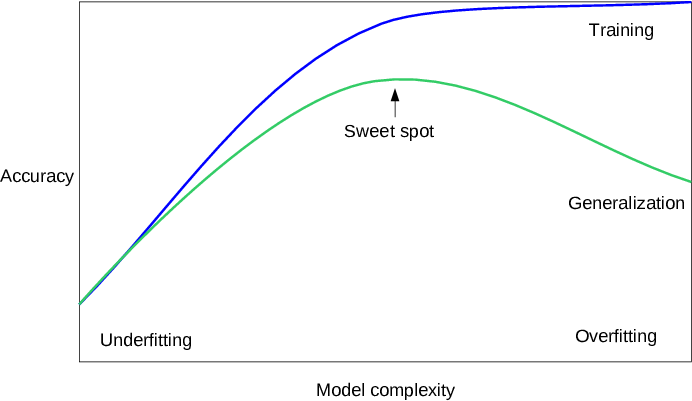
\includegraphics[width=0.7\textwidth]{img/overfitting-underfitting}
	\caption{Trade-off entre complexidade do modelo e generalização}
	\label{fig:overfitting-underfitting}
\end{figure}

A Figura~\ref{fig:overfitting-underfitting} ilustra estes problemas. Quando o modelo se ajusta demais aos dados (curva em azul), a complexidade aumenta e a generalização diminui. O ponto ótimo (representado pelo \textit{sweet pot}) possui uma complexidade intermediária, capaz de responder com qualidade aos dados existentes e novos.

\section{Repositório de dados}

No projeto e desenvolvimento de métodos de aprendizagem de máquina, é comum o uso de conjuntos de dados comuns e disponíveis à comunidade científica. Isso facilita a execução de experimentos, pois o projetista não precisa se preocupar em preparar diferentes conjuntos de dados, bem como permite a comparação de distintas técnicas em um número maior de bases de dados.O repositório mais conhecido é o UCI, que pode ser acessado no endereço \url{http://archive.ics.uci.edu/ml}. Este repositório possui 383 conjuntos de dados que podem ser utilizados para aplicação de diferentes métodos de aprendizagem de máquina. Para cada conjunto de dados, são apresentadas suas informações básicas (número de instâncias, números de atributos, tarefa de aprendizagem associada, etc.), uma descrição sobre a origem dos dados e artigos científicos relacionados.

O conjunto de dados das espécies de íris, por exemplo, pode ser consultado em \url{http://archive.ics.uci.edu/ml/datasets/Iris}. Ele possui 150 instâncias, cada uma com 4 atributos e a tarefa de aprendizagem é a classificação. Com base nos 4 atributos de entrada, a tarefa consiste em determinar uma entre as três classes possíveis (\textit{íris setosa}, \textit{íris versicolor} e \textit{íris virgínica}). Os dados são disponibilizados em um arquivo com extensão \texttt{.data} e possuem uma estrutura simples que facilita sua leitura. O arquivo \texttt{iris.data} apresenta o valor de cada atributo separado por vírgula, com a classe sendo apresentada por último (Figura~\ref{fig:estrutura-dados-iris}).

\begin{figure}[h]
\framebox[\textwidth]{
	\hspace{1em}
	\vbox{
		\texttt{5.1,3.5,1.4,0.2,Iris-setosa} \\
		\texttt{4.9,3.0,1.4,0.2,Iris-setosa} \\
		\texttt{4.7,3.2,1.3,0.2,Iris-setosa} \\
		\texttt{4.6,3.1,1.5,0.2,Iris-setosa} \\
		\texttt{5.0,3.6,1.4,0.2,Iris-setosa} \\
		\texttt{5.4,3.9,1.7,0.4,Iris-setosa} \\
		$\vdots$
	}
}

\caption{Estrutura do conjunto de dados \texttt{iris}}
\label{fig:estrutura-dados-iris}
\end{figure}

\section{Recursos disponíveis}

Existem alguns softwares que implementam métodos de aprendizagem de máquina e possibilitam o seu uso sem a necessidade de escrita de código. O mais conhecido deles é o Weka~\footnote{\url{http://www.cs.waikato.ac.nz/ml/weka}}. O software disponibiliza a implementação de diversos algoritmos de aprendizagem de máquina, bem como tarefas de pré-processamento de dados, visualização gráfica e avaliação dos resultados. Além disso, ele permite a integração com Java, podendo ser utilizado como uma biblioteca com os algoritmos. Por ser um software popular, possui boa documentação e uma ativa comunidade de usuários. Consulte a documentação em \url{http://www.cs.waikato.ac.nz/ml/weka/documentation.html}.

Uma boa opção para desenvolvedores Python é a biblioteca \texttt{scikit-learn}~\footnote{\url{http://scikit-learn.org}}. Esta biblioteca é apresentada e utilizada em~\cite{MullerAndGuido2017}, o que auxilia no seu entendimento, pois a obra apresenta muitos exemplos para diferentes tarefas de aprendizagem de máquina. Esta biblioteca implementa vários algoritmos e, juntamente com as bibliotecas \texttt{scipy}, \texttt{numpy} e \texttt{matplotlib}, permite a análise de resultados e a visualização gráfica dos mesmos.

Para desenvolvedores Java existem outras bibliotecas além do Weka. Uma das mais conhecidas é o \texttt{Java-ML}~\footnote{\url{http://java-ml.sourceforge.net}} (\textit{Java Machine Learning}). Esta biblioteca implementa uma série de algoritmos de aprendizagem de máquina e fornece uma interface simples para seu uso. A documentação é bastante abrangente e existem vários tutoriais para conhecer e utilizar os recursos disponíveis. Mais detalhes sobre as bibliotecas e ferramentas disponíveis, bem como o uso de Java na aprendizagem de máquina podem ser consultados em~\cite{Kaluza2016} e~\cite{KamathAndChoppella2017}.

\section{Exercícios}

\resetexercisenumbering

\begin{exercise}
Pesquise aplicações reais onde algoritmos de aprendizagem de máquina são empregados. Comente sobre quais técnicas são utilizadas e quais os resultados obtidos por tais aplicações.
\end{exercise}

\begin{exercise}
Pesquise e explique o conceito de aprendizado semi-supervisionado, comentando sobre os métodos existentes e suas aplicações.
\end{exercise}

\begin{exercise}
Considere a tarefa de um ser humano de aprender a jogar tênis. Explique como esse processo pode ser comparado aos conceitos de aprendizagem de máquina. Descreva as percepções e ações do indivíduo e as subfunções que ele está tentando aprender. Trata-se de uma aprendizagem supervisionada ou de uma aprendizagem por reforço?
\end{exercise}

\begin{exercise}
Cada professor possui um bolsista, responsável por auxiliar nas atividades das disciplinas por ele ministradas. Considere um bolsista que, com base no gabarito fornecido pelo professor, corrija as provas de uma disciplina. Como seria um bolsista que aprendeu a corrigir provas nas situações de \textit{underfitting} e \textit{overfitting}.
\end{exercise}
\chapter{Aprendizado supervisionado}
\label{cap:aprendizado-supervisionado}

\framebox[\textwidth]{
	\hspace{1em}
	\vbox{
		\textbf{Leitura obrigatória:}
		\begin{itemize}
			\item \cite{FaceliEtAl2011} -- Cap. 4 (Métodos Baseados em Distâncias).
			\item \cite{Mitchell1997} -- Cap. 3 (Decision Tree Learning).
		\end{itemize}
		
		\textbf{Leitura complementar:}
		\begin{itemize}
			\item \cite{RusselAndNorvig2010} -- Cap. 18 (Aprendendo através de exemplos).
			\item \cite{MullerAndGuido2017} -- Cap. 2 (Supervised Learning).
		\end{itemize}
	}
}

\section{Visão geral}

Conforme discutido no Capítulo~\ref{cap:conceitos-basicos-aprendizagem-maquina}, o aprendizado supervisionado é aplicado a tarefas preditivas de classificação e regressão. As técnicas de aprendizado supervisionado se baseiam em um conjunto de dados rotulados e tem por objetivo aprender uma hipótese ou função que relacione os atributos de entrada com o atributo de saída. Com isso, o valor do atributo de saída de uma nova entrada pode ser estimada.

A aprendizagem é chamada supervisionada pois os dados servem como exemplos, que são utilizados durante o processo de aprendizagem. Com isso, cada tentativa de predição é avaliada por um ``supervisor'', o qual se baseia nos dados rotulados. Este paradigma exige um esforço humano em rotular um conjunto de dados para a aprendizagem, mas produzem hipóteses que podem ser utilizadas em tarefas de predição futuras. Os dados rotulados utilizados na indução da hipótese são chamados de \textbf{conjunto de treinamento}, enquanto os dados utilizados para validar a hipótese induzida são chamados de \textbf{conjunto de teste}. O processo de aprendizagem, portanto, pode ser chamado de \textbf{treinamento} do modelo.

Após realizado o treinamento do modelo, temos um \textbf{estimador}, capaz de predizer o valor do atributo alvo de novos e desconhecidos dados. Caso o atributo alvo toma valores de um domínio de valores nominais, temos a tarefa de \textbf{classificação} e chamamos o modelo de \textbf{classificador}. Caso o atributo alvo toma valores em um intervalo contínuo e ordenado, temos uma tarefa de \textbf{regressão} e chamamos o modelo de \textbf{regressor}.

A Tabela~\ref{tab:exemplo-classificacao} apresenta um exemplo de classificação. Trata-se de parte do conjunto de dados chamado \texttt{iris}, que contém registros do tamanho (comprimento e largura) da pétala e da sépala de diferentes flores íris. Com base nos quatro atributos de entrada, a tarefa consiste em classificar as flores segundo sua espécie: íris setosa, íris versicolor ou íris virgínica. Perceba que o atributo alvo (espécie) consiste em um valor nominal (conjunto discreto) e, portanto, trata-se de uma tarefa de classificação.

\begin{table}[h]
	\centering
	
	\begin{tabular}{rrrrl}
		\hline
		\textbf{Comp. (P)} & \textbf{Larg. (P)} & \textbf{Comp. (S)} & \textbf{Larg. (S)} & \textbf{Espécie} \\
		\hline
		5,1 & 3,5 & 1,4 & 0,2 & Setosa \\
		4,9 & 3,0 & 1,4 & 0,2 & Setosa \\
		7,0 & 3,2 & 4,7 & 1,4 & Versicolor \\
		6,4 & 3,2 & 4,5 & 1,5 & Versicolor \\
		6,3 & 3,3 & 6,0 & 2,5 & Virgínica \\
		5,8 & 2,7 & 5,1 & 1,9 & Virgínica \\
		$\vdots$ & $\vdots$ & $\vdots$ & $\vdots$ & $\vdots$ \\
		\hline
	\end{tabular}
	
	\caption{Exemplo de classificação das espécies de íris}
	\label{tab:exemplo-classificacao}
\end{table}

A Tabela~\ref{tab:exemplo-regressao} apresenta um exemplo de regressão. Trata-se de um conjunto de dados chamado \texttt{swiss}, que contém registros estatísticos de uma população, como educação e taxa de fertilidade. A tarefa é definir, com base nos atributos de entrada, a taxa de mortalidade da população (atributo alvo). Trata-se de um problema de regressão, pois o atributo alvo pode assumir qualquer valor em um intervalo contínuo.

\begin{table}[h]
	\centering
	
	\begin{tabular}{rrrrr}
		\hline
		\textbf{Fertilidade} & \textbf{Agricultura} & \textbf{Educação} & \textbf{Renda} & \textbf{Mortalidade} \\
		\hline
		80,2 & 17,0 & 12 & 9,9 & 22,2\\
		83,1 & 45,1 & 9 & 84,8 & 22,2\\
		92,5 & 39,7 & 5 & 93,4 & 20,2\\
		85,8 & 36,5 & 7 & 33,7 & 20,3\\
		76,9 & 43,5 & 15 & 5,2 & 20,6\\
		$\vdots$ & $\vdots$ & $\vdots$ & $\vdots$ & $\vdots$ \\
		\hline
	\end{tabular}
	
	\caption{Exemplo de regressão da taxa de mortalidade}
	\label{tab:exemplo-regressao}
\end{table}

Finalmente, a Figura~\ref{fig:exemplo-classificacao-regressao} ilustra as tarefas de classificação e regressão. Na primeira imagem, a classe do objeto é determinada em função dos valores das duas características de entrada, que são representadas pelos eixos $x$ e $y$. Na segunda imagem, o eixo $x$ apresenta o valor de uma característica, enquanto o eixo $y$ mostra o valor do atributo alvo. A tarefa consiste em determina a função que mapeia o valor no atributo de entrada para o valor do atributo alvo.

\begin{figure}[h]
	\centering
	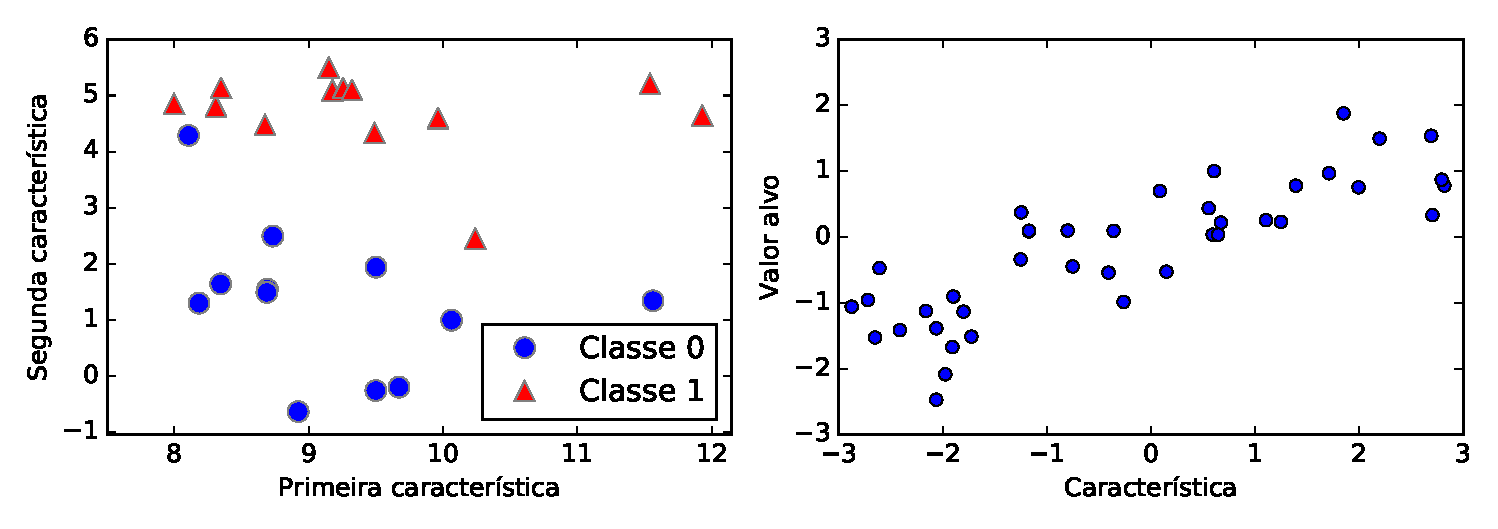
\includegraphics[width=\textwidth]{img/exemplo-classificacao-regressao}
	\caption{Ilustração das tarefas de classificação e regressão}
	\label{fig:exemplo-classificacao-regressao}
\end{figure}

\section{Algoritmo \textit{k}NN -- \textit{k}-Nearest Neighbors}

O algoritmo do $k$NN (do inglês $k$-Nearest Neighbors), ou $k$-Vizinhos Mais Próximos é um método de aprendizagem de máquina baseado em instância, também classificado por muitos autores como uma técnica de \textbf{raciocínio baseado em casos}. O $k$NN considera a proximidade dos dados (das instâncias) para realização da predição. Ele consiste na técnica mais simples de aprendizagem de máquina e pode ser aplicado tanto para classificação como para regressão. A ideia principal é de que \textit{objetos relacionados ao mesmo conceito são semelhantes entre si}. O $k$NN é uma técnica simples pois não aprende um modelo compacto para os dados, mas memoriza todos eles durante a fase de treinamento, para então classificar novos dados com base na proximidade dos existentes.

\subsection{Esquema geral}

A distância entre dois objetos pode ser determinada pela distância euclidiana, calculada com base nos valores dos seus atributos de entrada. Seja $x_i$ o valor do atributo $i$ do objeto $x$ e $d$ o número de atributos do objeto, a distância entre dois objetos $a$ e $b$ pode ser definida como:
$$
d(a, b) = \sqrt{\sum_{i=1}^{d} (a_i - b_i)^2}
$$

\textbf{Observações:}
\begin{itemize}
	\item Esta medida é chamada de \textbf{distância euclidiana}. Existem outras medidas que podem ser aplicadas, como a \textit{distância de Manhattan} ou a \textit{distância Supremum}.
	\item Caso o atributo $i$ seja qualitativo (nominal, por exemplo), $a_i - b_i = 1$, caso $a_i \neq b_i$ e 0, caso contrário. Neste caso, é comum eliminar a radiciação do cálculo da distância.
	\item Existem outras medidas de distância para atributos qualitativos, como a \textit{separação angular} e a \textit{correlação de pearson}.
\end{itemize}

\insertspace

O algoritmo kNN estima o valor do atributo alvo de um novo objeto com base nos seus $k$ vizinhos mais próximos. Ou seja, dado um novo objeto, o algoritmo calcula a distância entre si e cada objeto do conjunto de treinamento, selecionando os $k$ mais próximos. No caso da classificação, o algoritmo atribui ao novo objeto a classe destes vizinhos. Caso ocorra divergências, o algoritmo seleciona a classe mais frequente, chamada de classe majoritária. Esta estratégia é chamada de \textbf{votação}. No caso da regressão, o algoritmo calcula a média dos valores dos $k$ vizinhos mais próximos, ou ainda outra medida estatística (como a mediana, por exemplo).

O caso mais simples é o algoritmo 1NN, que considera apenas o vizinho mais próximo e seleciona sua classe para a predição (ou o valor numérico do seu atributo alvo). A Figura~\ref{fig:exemplo-1nn} mostra um conjunto de dados onde os dados de treinamento são apresentados como círculos em azul (para a classe 0) e triângulos em vermelho (para a classe 1). Os dados de teste são apresentados como estrelas e sua cor indica a classe que foi atribuída a cada um. Como podemos perceber, a classe do vizinho mais próximo é atribuída ao novo dado.

\begin{figure}[h]
	\centering
	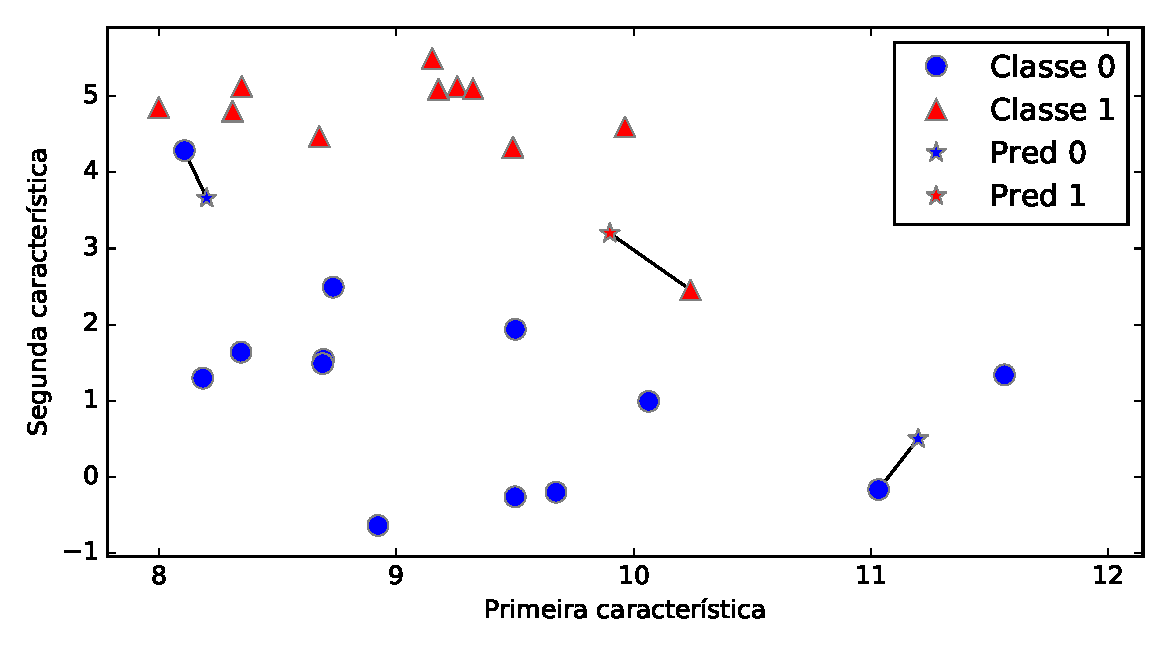
\includegraphics[width=0.7\textwidth]{img/exemplo-1nn}
	\caption{Exemplo de aplicação do algoritmo 1NN}
	\label{fig:exemplo-1nn}
\end{figure}

\begin{figure}[h]
	\centering
	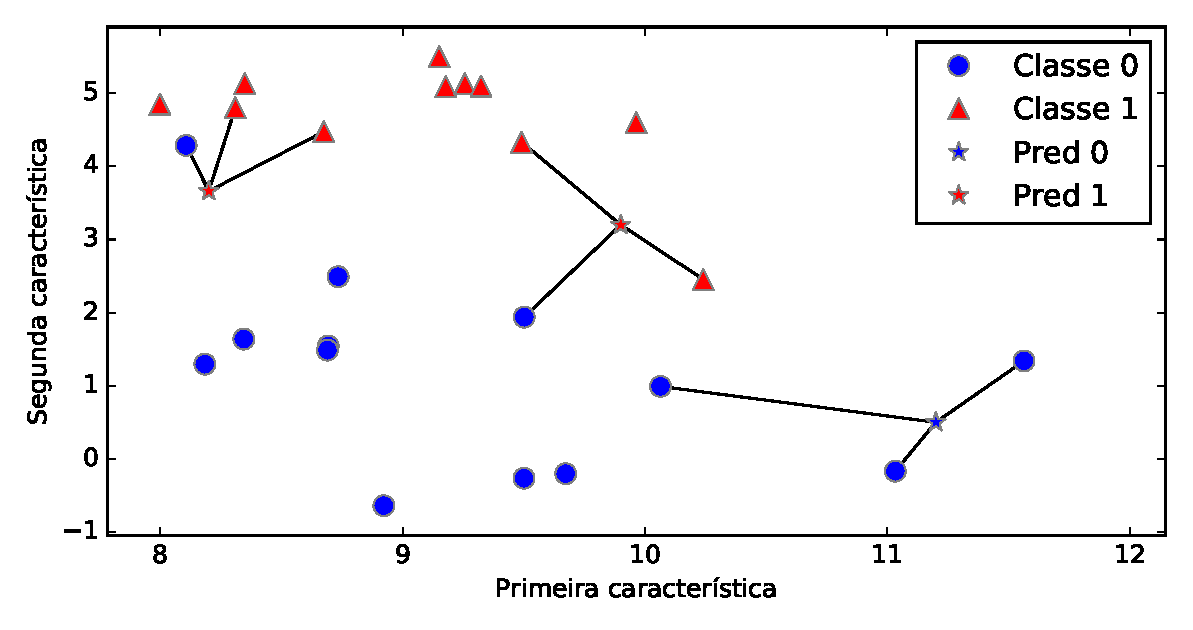
\includegraphics[width=0.7\textwidth]{img/exemplo-3nn}
	\caption{Exemplo de aplicação do algoritmo 3NN}
	\label{fig:exemplo-3nn}
\end{figure}

Ao executar o algoritmo com um número maior de vizinhos, a predição torna-se mais precisa. A Figura~\ref{fig:exemplo-3nn} mostra o mesmo conjunto de dados sendo utilizado para a predição de três novos dados usando o algoritmo de 3NN. Neste caso, a classe é atribuída conforme os 3 vizinhos mais próximos, utilizando a estratégia de votação para resolver divergências. Perceba que a estrela do canto superior esquerdo, apesar de estar mais próxima a um objeto da classe 0, possui maior similaridade com a classe 1, pois a região superior é dominada por objetos desta classe. Esta característica só foi identificada com o uso de um maior número de vizinhos. Por outro lado, deve-se tomar cuidado para não atribuir um número muito elevado de vizinhos, gerando sub e sobreajuste. Cabe ressaltar que em tarefas de classificação binária, onde existem apenas duas classes possíveis, um número ímpar de vizinhos deve ser utilizado para evitar empates.

A Figura~\ref{fig:exemplo-1nn-regressao} mostra a aplicação do algoritmo 1NN para uma tarefa de regressão. O eixo $x$ mostra a característica, enquanto o eixo $y$ mapeia o valor do atributo alvo. O valor da predição é igual ao vizinho mais próximo do dado a ser estimado. A Figura~\ref{fig:exemplo-3nn-regressao} mostra a mesma tarefa sendo executada por um algoritmo 3NN. Dado o maior número de vizinhos, o valor alvo é melhor estimado, como pode ser percebido no primeiro dado de teste (mais a esquerda).

\begin{figure}[h]
	\centering
	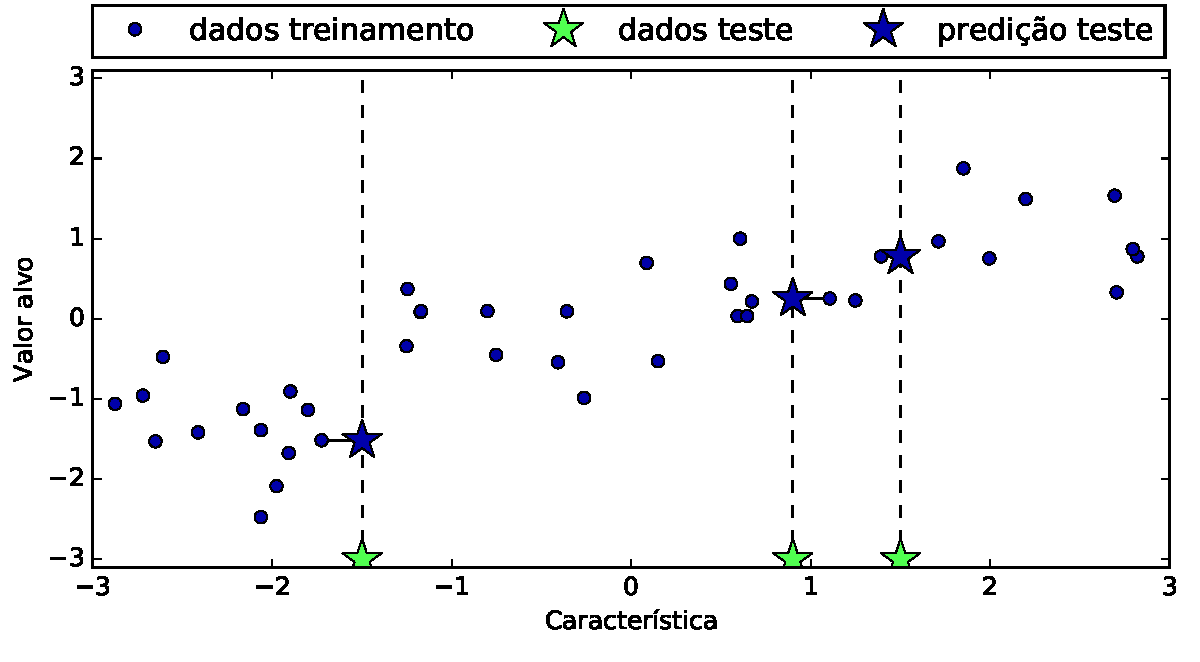
\includegraphics[width=0.85\textwidth]{img/exemplo-1nn-regressao}
	\caption{Exemplo de aplicação do algoritmo 1NN para regressão}
	\label{fig:exemplo-1nn-regressao}
\end{figure}

\begin{figure}[h!]
	\centering
	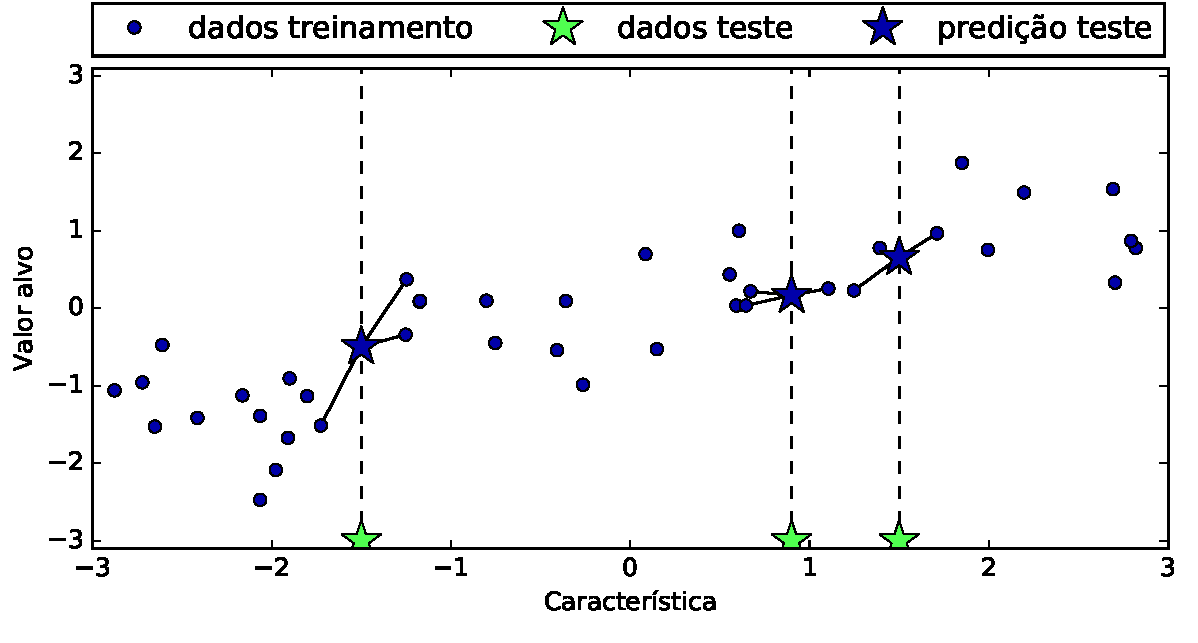
\includegraphics[width=0.85\textwidth]{img/exemplo-3nn-regressao}
	\caption{Exemplo de aplicação do algoritmo 3NN para regressão}
	\label{fig:exemplo-3nn-regressao}
\end{figure}

A medida de similaridade dos objetos é impactada pela ordem de grandeza dos atributos de entrada. Considere um atributo $x$ que assume um valor no intervalo $[1, 10]$, e um segundo atributo $y$ que assume um valor no intervalo $[1, 1000]$. Agora considere que um objeto possui os seguintes valores de atributos $(x, y) = (1, 1)$. Se definirmos um segundo objeto com valores $(10, 10)$, temos que este objeto é muito distante do primeiro ao considerar o atributo $x$, mas bastante próximo ao considerar o atributo $y$. No entanto, a diferença absoluta entre os valores dos atributos de cada objeto é a mesma (10). Ou seja, o valor 10 significa distância máxima com relação ao atributo $x$, e proximidade com relação ao atributo $y$. Ao considerar apenas valores absolutos, o método pode induzir uma hipótese de baixa qualidade por conta da sensibilidade em relação à ordem de grandeza de diferentes atributos. Por isso, é recomendável que todos os atributos quantitativos passem por um processo de \textbf{normalização} antes de executar o algoritmo $k$NN.

A normalização pode ser feita selecionando, a partir dos dados de treinamento, o maior valor apresentado. Este valor passa a ser 1 e todos os demais são atualizados proporcionalmente. Por exemplo, se o maior valor de um atributo é 100, este passa a valer 1 e o valor 75 passa a valer 0,75, e assim por diante. Com isso, todos os atributos quantitativos terão intervalo $[0, 1]$, resolvendo o problema da sensibilidade à grandeza dos atributos.

\textbf{Observação:} além da normalização, outra medida de pré-processamento recomendada é a eliminação de atributos irrelevantes. Por exemplo, para definir se o paciente é \textit{doente} ou \textit{saudável}, não importa saber o valor do atributo \texttt{nome}.

\subsection{Análise do algoritmo}

Para um algoritmo $k$NN, podemos definir as áreas do conjunto de dados que resultarão na predição de cada classe. Isto é, se um novo dado se encontrar em uma determinada área, ele receberá a classe correspondente. A Figura~\ref{fig:analise-knn} mostra as áreas para as classes 0 e 1 para diferentes valores de $k$. Como pode ser observado, a predição com 9 vizinhos divide o conjunto de dados utilizando uma fronteira de decisão mais simples e, por isso, possui uma melhor generalização.

\begin{figure}[h]
	\centering
	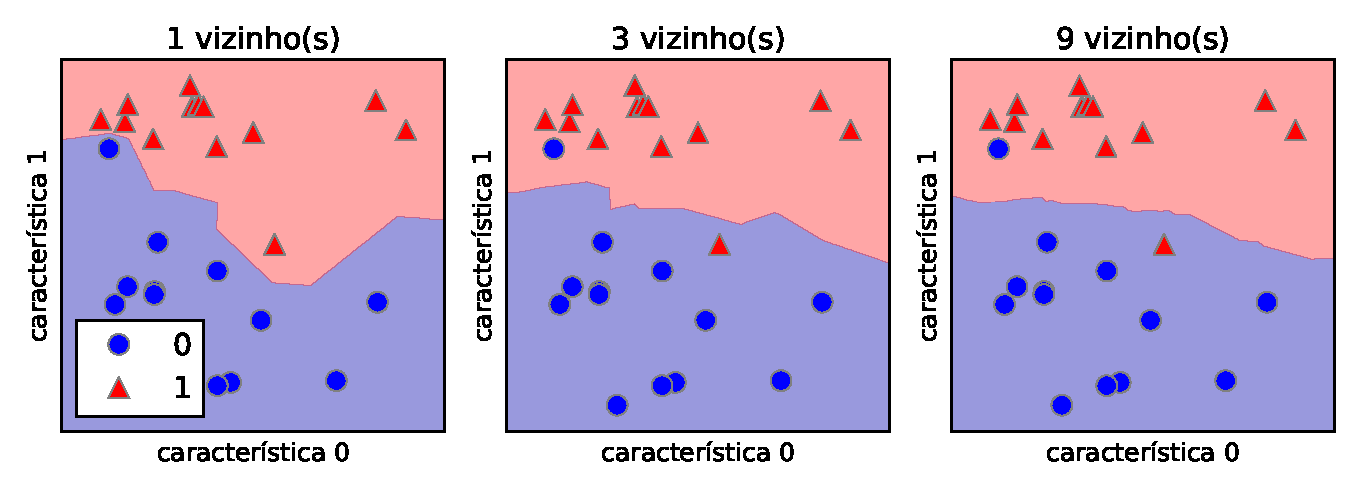
\includegraphics[width=\textwidth]{img/analise-knn}
	\caption{Análise do algoritmo KNN para classificação com diferentes valores de $k$}
	\label{fig:analise-knn}
\end{figure}

A mesma ideia se aplica para problemas de regressão. A Figura~\ref{fig:analise-knn-regressao} mostra a execução do algoritmo com diferentes valores de vizinhos. Ao utilizar apenas 1 vizinho, a predição se ajusta aos dados de treinamento. O \textit{score} de treinamento é 1,00, enquanto o \textit{score} do teste é baixo (0,35). Ao aumentar o número de vizinhos, o \textit{score} de treinamento diminui, pois o modelo deixa de se ajustar perfeitamente aos dados de treinamento, mas aumenta a capacidade de generalização, o que é percebido no crescimento do \textit{score} de teste. Em outras palavras, com um maior número de vizinhos a predição produz uma curva que não possui predição exata para os dados de treinamento, mas generaliza melhor para novos dados.

\begin{figure}[h]
	\centering
	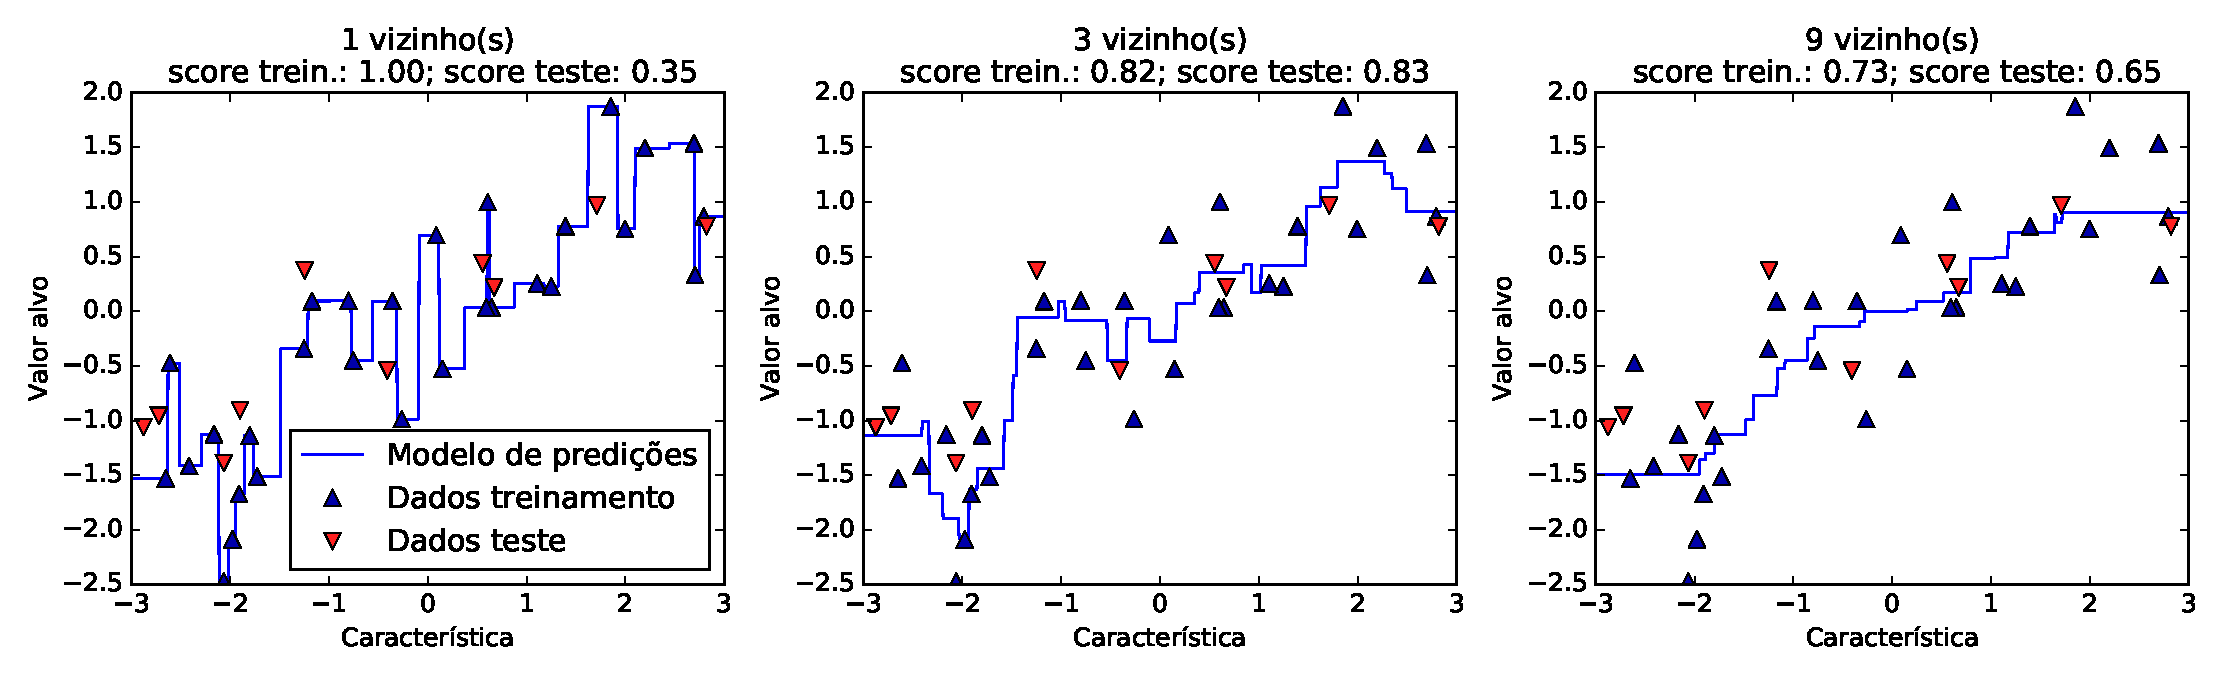
\includegraphics[width=\textwidth]{img/analise-knn-regressao}
	\caption{Análise do algoritmo KNN para regressão com diferentes valores de $k$}
	\label{fig:analise-knn-regressao}
\end{figure}

Apesar dessas análises indicarem problemas ao se utilizar um número muito baixo de vizinhos, adotar um número muito elevado também deve ser evitado. Se utilizarmos $k$ igual ao número total de objetos de treinamento, toda a classificação será baseada na classe majoritária do conjunto de treinamento, enquanto toda a regressão resultará na média do valor do atributo alvo de todos os dados de treinamento. Obter um bom desempenho do $k$NN consiste em determinar um valor adequado para $k$. Esta situação é demonstrada na Figura~\ref{fig:acuracia-knn-diferentes-k}, que apresenta os resultados do algoritmo $k$NN para diferentes valores de $k$. A curva em azul mostra a acurácia da predição sobre o conjunto de treinamento, enquanto a curva tracejada em vermelho mostra a acurácia no conjunto de teste. Valores pequenos de $k$ levam a um sobreajuste, pois a predição é boa para o conjunto de treinamento e ruim para o conjunto de teste. Valores muito elevados de $k$ levam a um subajuste, onde a predição não é boa em nenhum dos casos. Concluindo, um valor intermediário é desejado e deve ser obtido experimentalmente.

\begin{figure}[h]
	\centering
	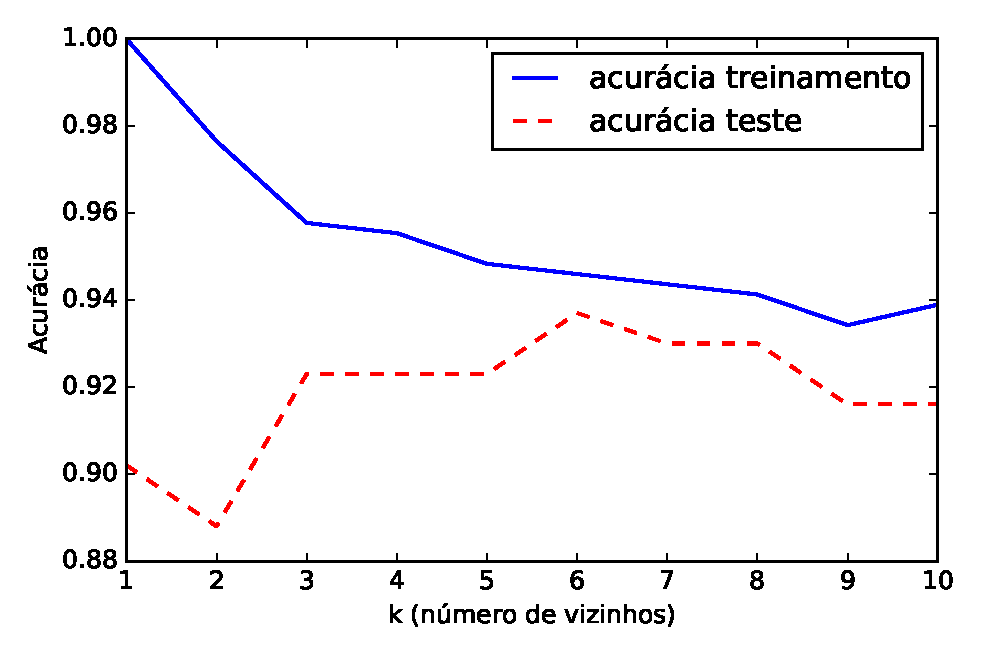
\includegraphics[width=0.75\textwidth]{img/acuracia-knn-diferentes-k}
	\caption{Acurácia do algoritmo $k$NN para diferentes valores de $k$}
	\label{fig:acuracia-knn-diferentes-k}
\end{figure}

Entre os pontos positivos do algoritmo de $k$NN, destacam-se:
\begin{itemize}
	\item Simplicidade.
	\item A fase de treinamento é simples.
	\item É aplicável a problemas complexos e, em geral, apresenta bom desempenho.
	\item Naturalmente incremental: se existem novos dados de exemplo, basta incluir no conjunto de treinamento.
\end{itemize}

\insertspace

Entre os pontos negativos do algoritmo de $k$NN, destacam-se:
\begin{itemize}
	\item Não retorna uma representação compacta dos dados.
	\item A fase de teste é custosa.
	\item É afetado com a presença de dados redundantes e atributos irrelevantes.
\end{itemize}

\subsection{\textit{k}NN ponderado}

Uma extensão do algoritmo $k$NN consiste em ponderar a contribuição de cada vizinho, de tal forma que vizinhos mais próximos tenham maior influência na determinação do valor alvo do elemento analisado. Uma prática comum é adotar o inverso do quadrado da distância entre o elemento e o vizinho. Ou seja, sendo $a$ o elemento a ser analisado e $b$ um dos vizinhos mais próximos, o peso $w_b$ com o qual a contribuição de $b$ será ponderada é dado por

$$
w_b = \frac{1}{d(x_a, x_b)^2}
$$

Com o uso de uma ponderação baseada na distância, é possível aumentar o valor de $k$ sem sofrer com overfitting. É possível, inclusive, utilizar todos os exemplos de treinamento para a classificação de uma instância, pois vizinhos distantes possuem pouca influência no resultado da classificação. Perceba que utilizar todo o conjunto de treinamento sem aplicar ponderação implica em uma classificação igual à classe majoritária, o que evidentemente não é desejado. O mesmo efeito ocorre na regressão, onde o valor médio de todo o conjunto de treinamento seria atribuído a qualquer instância de teste.

O único fator que impede adotar todo o conjunto de treinamento no $k$NN ponderado é o aumento na complexidade de computação. Se o conjunto de treinamento for grande, o tempo de processamento acaba crescendo em demasia. Uma prática comum é adotar o maior número possível de vizinhos, capaz de ser processado em tempo razoável. Quando a tarefa considera todos os exemplos de treinamento, chamamos de \textbf{método global}. Quando um menor número de exemplos de treinamento é adotado, chamamos de \textbf{método local}.

\section{Árvores de decisão}

Árvores de decisão são muito comuns e largamente utilizadas para inferência indutiva. Sistemas inteligentes baseados em árvores de decisão possuem diversas aplicações de sucesso, como diagnóstico médico, identificação de riscos em investimentos financeiros ou análise de crédito. Esta técnica é utilizada principalmente para tarefas de classificação, mas existem extensões que permitem sua aplicações para tarefas de regressão, ainda que menos comuns. Esta seção apresenta os conceitos relacionados às árvores de decisão e detalha o funcionamento dos seus algoritmos de indução com o foco em tarefas de classificação.

\subsection{Esquema geral}
\label{sec:arvores-decisao-esquema-geral}

Uma árvore de decisão classifica uma nova instância analisando seus atributos. Cada nó da árvore testa um atributo e cada ramo que descende do nó corresponde a um possível valor para ele. Para classificar uma instância, iniciam-se pelo nó raiz da árvore, testando primeiro atributo. De acordo com o valor, a busca desce ao nó correspondente e repete-se o processo até chegar em uma das folhas. As folhas fornecem as possíveis classes.

A Figura~\ref{fig:exemplo-arvore-decisao} apresenta uma árvore de decisão que avalia as condições meteorológicas de uma manhã de sábado, decidindo sobre jogar ou não tênis. Cada nó avalia uma característica e os ramos representam os valores possíveis. As folhas apresentam a decisão, ou seja, as classes \textit{Sim} (jogar) ou \textit{Não} (não jogar). Por exemplo, a instância
\begin{center}
	$\langle$ Clima = Ensolarado, Temperatura = Quente, Umidade = Alta, Vento = Forte $\rangle$
\end{center}
seria classificada pelo ramo da esquerda, que seleciona o atributo \textit{clima} como \textit{ensolarado} e a \textit{umidade} como \textit{alta} (como resultado, a predição é \textit{Jogar tênis = não}). Neste caso, o atributo \textit{vento} não foi utilizado. Além disso, a árvore não considera o atributo \textit{temperatura} para a classificação.

\begin{figure}[h]
	\centering
	\tikzstyle{no} = [draw, rectangle, inner sep=7pt, minimum width=2.5cm]
	\tikzstyle{folha} = [draw, ellipse, inner sep=5pt, minimum width=2cm, dashed]
	\tikzstyle{texto} = [pos=.5, fill=white]
	
	\begin{tikzpicture}
		\node[no] (clima) at (0,0) {Clima};
		\node[no] (umidade) at (-4,-2.5) {Umidade};
		\node[no] (vento) at (4,-2.5) {Vento};
		\node[folha] (sim1) at (0,-2.5) {Sim};
		\node[folha] (nao1) at (-6,-5) {Não};
		\node[folha] (sim2) at (-2,-5) {Sim};
		\node[folha] (nao2) at (2,-5) {Não};
		\node[folha] (sim3) at (6,-5) {Sim};
		
		\draw (clima) -- (umidade) node[texto] {\small Ensolarado};
		\draw (clima) -- (vento) node[texto] {\small Chuvoso};
		\draw (clima) -- (sim1) node[texto] {\small Nublado};
		\draw (umidade) -- (nao1) node[texto] {\small Alta};
		\draw (umidade) -- (sim2) node[texto] {\small Normal};
		\draw (vento) -- (nao2) node[texto] {\small Forte};
		\draw (vento) -- (sim3) node[texto] {\small Fraco};
	\end{tikzpicture}
	
	\caption{Árvore de decisão para decidir sobre jogar tênis}
	\label{fig:exemplo-arvore-decisao}
\end{figure}

\insertspace

Podemos representar uma árvore de decisão como um conjunto de regras do tipo \texttt{se--então}. A árvore da Figura~\ref{fig:exemplo-arvore-decisao} mapeia as seguintes regras:

\insertspace

\framebox[\textwidth]{
	\hspace{1em}
	\vbox{
		\textbf{SE} \textit{Clima = Ensolarado} \textbf{E} \textit{Umidade = Alta} \textbf{ENTÃO} \textit{Jogar tênis = Não}
		
		\textbf{SE} \textit{Clima = Ensolarado} \textbf{E} \textit{Umidade = Normal} \textbf{ENTÃO} \textit{Jogar tênis = Sim}
		
		\textbf{SE} \textit{Clima = Nublado} \textbf{ENTÃO} \textit{Jogar tênis = Sim}
		
		\textbf{SE} \textit{Clima = Chuvoso} \textbf{E} \textit{Vento = Forte} \textbf{ENTÃO} \textit{Jogar tênis = Não}
		
		\textbf{SE} \textit{Clima = Chuvoso} \textbf{E} \textit{Vento = Fraco} \textbf{ENTÃO} \textit{Jogar tênis = Sim}
	}
}

\insertspace

Cada classe pode ainda ser representada como uma conjunção de disjunções dos valores dos atributos das instâncias. Por exemplo, a classe \textit{Jogar tênis = Sim} da árvore da Figura~\ref{fig:exemplo-arvore-decisao} pode ser representada por:

\insertspace

\framebox[\textwidth]{
	\hspace{1em}
	\vbox{
		\begin{tabular}{ll}
			& (Clima = Ensolarado $\wedge$ Umidade = Normal) \\
			$\vee$ & (Clima = Nublado) \\
			$\vee$ & (Clima = Chuvoso $\wedge$ Vento = Forte)
		\end{tabular}
	}
}

\insertspace

As árvores de decisão são apropriadas para uma grande variedade de problemas. Em especial, algumas características contribuem para uma melhor aplicabilidade da técnica:

\begin{itemize}
	\item Instâncias são representadas por pares \texttt{atributo--valor}.
	\item A função objetivo possui valores discretos (classificação).
	\item O conjunto de treinamento pode conter erros.
	\item O conjunto de treinamento pode conter dados faltantes.
\end{itemize}

\subsection{Indução de árvores de decisão}

Uma vez conhecido o funcionamento de uma árvore de decisão, o objetivo é induzi-la a partir de um conjunto de dados de treinamento. Ou seja, com base nos dados existentes, construir uma árvore de decisão capaz de classificar novos e desconhecidos dados. A estratégia de indução dessas árvores consiste em uma busca gulosa \textit{top-down} no espaço de possíveis árvores de decisão. Os principais algoritmos que implementam esta estratégia são o ID3~\citep{Quinlan1986} e seu sucessor C4.5~\citep{Quinlan1993}.

A estratégia básica para a indução de uma árvore de decisão é implementada pelo algoritmo ID3. O primeiro passo consiste em selecionar o melhor atributo para ser testado no nó raiz da árvore. Cada atributo é testado de acordo com alguma métrica estatística que determina o quão bem aquele atributo classifica (sozinho) o conjunto de dados. O melhor atributo é selecionado para o nó raiz e um ramo descendente é criado para cada valor possível do atributo. Os dados são então separados para cada ramo, conforme o valor apresentado para o atributo selecionado. Todo o processo é repetido para cada ramo, utilizando o subconjunto de dados correspondente até a construção completa da árvore. Este procedimento é apresentado no Algoritmo~\ref{alg:id3}.

\begin{algorithm}[h]
	\DontPrintSemicolon
	\Entrada{\textit{exemplos -- $S$, atributo alvo -- $t$, atributos -- $A$}}
	\Saida{\textit{árvore de decisão}}
	
	\Inicio{
		\Se{todos os exemplos $s \in S$ são da mesma classe $c$}{
			\Retorna nó \textit{raiz}, que é uma folha com decisão $c$\;
		}
		
		\Se{$A = \emptyset$}{
			\Retorna nó \textit{raiz} com decisão igual à classe mais comum de $t$ em $S$\;
		}

		\textit{raiz.teste} $ \gets $ atributo $a \in A$ que melhor classifica $S$\;
		\Para{cada possível valor $v$ de \textit{raiz.teste}}{
			$S_v \gets $ subconjunto de $S$ em que $raiz.teste.valor = v$\;
			Adiciona um ramo ao nó \textit{raiz}\;
			Conecta neste ramo o resultado de ID3($S_v$, $t$, $A \setminus \{raiz.teste\}$)\;
		}
		
		\Retorna \textit{raiz}\;
	}
	
	\caption{Pseudocódigo para o algoritmo de indução de árvores ID3}
	\label{alg:id3}
\end{algorithm}

Perceba que o ID3 é aplicado apenas a problemas de classificação, isto é, quando o atributo alvo assume valores de um conjunto discreto de possibilidades. Além disso, os atributos devem ser discretos, pois ele testa todas as possibilidades de valores para cada atributo. Antes de discutir extensões do ID3 para contornar estas restrições, é importante entender a estratégia de seleção de atributos, ou seja, como a qualidade dos atributos é avaliada. Para isso, utiliza-se duas métricas: \textbf{entropia} e \textbf{ganho de informação}.

\subsection{Entropia e ganho de informação}

Estas métricas tem por objetivo avaliar o quão bem um atributo separa os exemplos para a classificação final. A \textbf{entropia} é uma medida bastante utilizada em teoria da informação e determina a \textit{impureza} dos dados. Dado um conjunto de dados de treinamento $S$, as possíveis classes $i = 1, 2, \hdots, c$ e a proporção $p_i$ dos exemplos com classe $i$, a entropia $E$ de $S$ é dada por
$$
E(S) = \sum_{i=1}^{c} -p_i \log_2 p_i.
$$

Considerando que $S$ é um conjunto completo dos dados de treinamento e $S_i$ são os exemplos cuja classe é $i$, a proporção $p_i = |S_i| / |S|$.

O \textbf{ganho de informação} define quanto a entropia será reduzida ao particionar o conjunto de exemplos $S$ de acordo com o atributo $A$. Sendo $S$ o conjunto completo de exemplos, $V$ o conjunto de valores possíveis do atributo $A$ e $S_v$ o conjunto de exemplos em que $A = v$, o ganho de informação é dado por
$$
G(S, A) = E(S) - \sum_{v \in V} \frac{|S_v|}{|S|} E(S_v)
$$

Isto é, o ganho de informação calcula a diferença de entropia entre o conjunto de dados original e aquele particionado em função do atributo $A$.

\subsection{Exemplo -- linguagens de programação}

Consideremos o problema da escolha de uma linguagem de programação para desenvolvimento de um software. A Tabela~\ref{tab:dados-linguagens-programacao} apresenta os dados relacionados a este problema. Os atributos definem a natureza da aplicação a ser desenvolvida: \textit{Comercial}, \textit{Internet} e \textit{Tempo Real}. O atributo alvo consiste na \textit{linguagem} de programação a ser escolhida.

\begin{table}[h]
	\centering
	
	\begin{tabular}{ccccl}
		\hline
		\textbf{\#} & \textbf{Comercial} & \textbf{Internet} & \textbf{Tempo Real} & \textbf{Linguagem} \\
		\hline
		1 & S & N & N & Delphi \\
		2 & S & N & S & C++ \\
		3 & S & S & N & Java \\
		4 & N & S & S & Java \\
		5 & N & N & S & C++ \\
		6 & N & S & N & Java \\
		\hline
	\end{tabular}
	
	\caption{Dados de treinamento para escolha de linguagem de programação}
	\label{tab:dados-linguagens-programacao}
\end{table}

\subsubsection{Cálculo da entropia}

O primeiro passo consiste em selecionar o nó raiz da árvore. Para isso, devemos calcular a entropia do conjunto $S = \{1, 2, 3, 4, 5, 6\}$. As classes são $i \in \{\text{Delphi}, \text{C++}, \text{Java}\}$. Logo,
\begin{align*}
	p_{\text{Delphi}} = \frac{|S_{\text{Delphi}}|}{S} &= \frac{1}{6} \\[10pt]
	p_{\text{C++}} = \frac{|S_{\text{C++}}|}{S} &= \frac{2}{6} \\[10pt]
	p_{\text{Java}} = \frac{|S_{\text{Java}}|}{S} &= \frac{3}{6}
\end{align*}

Com isso, o valor de entropia pode ser calculado como
\begin{align*}
	E(S) &= \sum_{i=1}^{c} -p_i \log_2 p_i \\[10pt]
	&= (-p_{\text{Delphi}} \log_2 p_{\text{Delphi}}) + (-p_{\text{C++}} \log_2 p_{\text{C++}}) + (-p_{\text{Java}} \log_2 p_{\text{Java}}) \\[10pt]
	&= \left( -\frac{1}{6} \log_2 \frac{1}{6} \right) + \left( -\frac{2}{6} \log_2 \frac{2}{6} \right) + \left( -\frac{3}{6} \log_2 \frac{3}{6} \right) \\[10pt]
	&= 0.43 + 0.528 + 0.5\\[10pt]
	&= 1.459
\end{align*}

\subsubsection{Cálculo do ganho de informação}

Uma vez conhecida a entropia do conjunto de dados, cada atributo é analisado, a fim de verificar qual apresenta o maior ganho de informação. Considerando o conjunto de dados $S = \{1, 2, 3, 4, 5, 6\}$, os atributos $A \in {\text{Comercial}, \text{Internet}, \text{Tempo Real}}$, cada atributo possui os possíveis valores $v \in \{\text{sim}, \text{não}\}$. Cada atributo possui $|S_\text{sim}| = 3$ e $|S_\text{não}| = 3$. Importante: os valores possíveis e o número de exemplos de cada valor poderiam ser diferentes para cada atributo.

Para o atributo \textit{Comercial}, a entropia para cada possível valor pode ser determinada com base nos valores de $p_i$, os quais são determinados para o novo conjunto de dados onde $A = v$, e não mais para todos os exemplos existentes. A entropia para \textit{Comercial = sim} é dada por
\begin{align*}
	E(S_\text{sim}) &= (-p_\text{Delphi} \log_2 p_\text{Delphi}) + (-p_\text{C++} \log_2 p_\text{C++}) + (-p_\text{Java} \log_2 p_\text{Java})\\[10pt]
	&= \left( - \frac{1}{3} \log_2 \frac{1}{3} \right) + \left( - \frac{1}{3} \log_2 \frac{1}{3} \right) + \left( - \frac{1}{3} \log_2 \frac{1}{3} \right)\\[10pt]
	&= 0.528 + 0.528 + 0.528\\[10pt]
	&= 1.584
\end{align*}

Da mesma forma, a entropia para \textit{Comercial = não} é calculada por 
\begin{align*}
	E(S_\text{não}) &= (-p_\text{Delphi} \log_2 p_\text{Delphi}) + (-p_\text{C++} \log_2 p_\text{C++}) + (-p_\text{Java} \log_2 p_\text{Java})\\[10pt]
	&= \left( - \frac{0}{3} \log_2 \frac{0}{3} \right) + \left( - \frac{1}{3} \log_2 \frac{1}{3} \right) + \left( - \frac{2}{3} \log_2 \frac{2}{3} \right)\\[10pt]
	&= 0.0 + 0.528 + 0.38\\[10pt]
	&= 0.918
\end{align*}

Finalmente, o ganho de informação pode ser calculado:
\begin{align*}
	G(S, \text{Comercial}) &= E(S) - \sum_{v \in V} \frac{|S_v|}{|S|} E(S_v)\\[10pt]
	&= E(S) - \left[ \frac{|S_\text{sim}|}{|S|} E(S_\text{sim}) + \frac{|S_\text{não}|}{|S|} E(S_\text{não}) \right]\\[10pt]
	&= 1.459 - \left[ \frac{3}{6} E(S_\text{sim}) + \frac{3}{6} E(S_\text{não}) \right]\\[10pt]
	&= 1.459 - \left[ \frac{3}{6} 1.58 + \frac{3}{6} 0.918 \right]\\[10pt]
	&= 1.459 - \left[ 0.792 + 0.459 \right]\\[10pt]
	&= 0.207
\end{align*}

O processo é repetido para cada atributo, resultando nos seguintes ganhos de informação:
\begin{itemize}
	\item $G(S, \text{Comercial}) = 0.207$
	\item $G(S, \text{Internet}) = 1$
	\item $G(S, \text{Tempo Real}) = 0.540$
\end{itemize}

\insertspace

\subsubsection{Seleção do atributo e construção da árvore}

Com base nos valores de ganho de informação, o melhor atributo para compor a raiz da árvore é \textit{Internet}. Ao selecionar este atributo, são criados os ramos \textit{sim} e \textit{não}. O ramo \textit{sim} possui o conjunto de exemplos $S_\text{sim} = \{3, 4, 6\}$, enquanto o ramo \textit{não} possui o conjunto de exemplos $S_\text{não} = \{1, 2, 5\}$. Para cada novo ramo, o mesmo processo é repetido considerando o subconjunto de exemplos que satisfaz o ramo em questão. A Figura~\ref{fig:arvore-parcial-linguagens-programacao-1} apresenta a árvore parcial (primeiro passo) com o nó raiz e os dois ramos construídos.

\begin{figure}[h]
	\centering
	\tikzstyle{no} = [draw, rectangle, inner sep=7pt, minimum width=2.5cm]
	\tikzstyle{folha} = [draw, ellipse, inner sep=5pt, minimum width=2cm, dashed]
	\tikzstyle{texto} = [pos=.5, fill=white]
	
	\begin{tikzpicture}
	\node[no] (internet) at (0,0) {Internet};
	\node (sim) at (-2,-2.5) {\textbf{?}};
	\node (nao) at (2,-2.5) {\textbf{?}};
	
	\draw (internet) -- (sim) node[texto] {\small S};
	\draw (internet) -- (nao) node[texto] {\small N};
	\end{tikzpicture}
	
	\caption{Árvore de decisão parcial (passo 1) para as linguagens de programação}
	\label{fig:arvore-parcial-linguagens-programacao-1}
\end{figure}

Ao selecionar o ramo \textit{Internet = S} para continuar a construção da árvore, percebemos que o subconjunto $S_\text{sim}$ possui todos os elementos com valor alvo \textit{Linguagem = Java}. Logo, não é necessário calcular a entropia e o ganho de informação destes exemplos, uma vez que todos possuem a mesma classe. Podemos, portanto, adicionar um nó folha neste ramo com a classe \textit{Java}. A árvore parcial (segundo passo) é apresentada na Figura~\ref{fig:arvore-parcial-linguagens-programacao-2}, incluindo a decisão sobre a classe \textit{Java}.

\begin{figure}[h]
	\centering
	\tikzstyle{no} = [draw, rectangle, inner sep=7pt, minimum width=2.5cm]
	\tikzstyle{folha} = [draw, ellipse, inner sep=5pt, minimum width=2cm, dashed]
	\tikzstyle{texto} = [pos=.5, fill=white]
	
	\begin{tikzpicture}
	\node[no] (internet) at (0,0) {Internet};
	\node[folha] (java) at (-2,-2.5) {Java};
	\node (nao) at (2,-2.5) {\textbf{?}};
	
	\draw (internet) -- (java) node[texto] {\small S};
	\draw (internet) -- (nao) node[texto] {\small N};
	\end{tikzpicture}
	
	\caption{Árvore de decisão parcial (passo 2) para as linguagens de programação}
	\label{fig:arvore-parcial-linguagens-programacao-2}
\end{figure}

Na sequência, devemos determinar o melhor atributo para testar os elementos do ramo \textit{Internet = N}. Consideremos os exemplos $S_\text{não} = \{1, 2, 5\}$ da Tabela~\ref{tab:dados-linguagens-programacao}. Estes dados estão apresentados na Tabela~\ref{tab:dados-linguagens-programacao-internet-nao}.

\begin{table}[h]
	\centering
	
	\begin{tabular}{ccccl}
		\hline
		\textbf{\#} & \textbf{Comercial} & \textbf{Internet} & \textbf{Tempo Real} & \textbf{Linguagem} \\
		\hline
		1 & S & N & N & Delphi \\
		2 & S & N & S & C++ \\
		5 & N & N & S & C++ \\
		\hline
	\end{tabular}
	
	\caption{Dados para escolha de linguagem de programação com \textit{Internet = N}}
	\label{tab:dados-linguagens-programacao-internet-nao}
\end{table}

\subsubsection{Próxima iteração}

Os valores de $p_i$ são determinados para $i \in \{\text{Delphi}, \text{C++}\}$, pois a classe \textit{Java} não está presente nos novos dados:
\begin{align*}
	p_{\text{Delphi}} = \frac{|S_{\text{Delphi}}|}{S} &= \frac{1}{3} \\[10pt]
	p_{\text{C++}} = \frac{|S_{\text{C++}}|}{S} &= \frac{2}{3} \\[10pt]
\end{align*}

Logo, a entropia é calculada como:
\begin{align*}
	E(S) &= \sum_{i=1}^{c} -p_i \log_2 p_i \\[10pt]
	&= (-p_{\text{Delphi}} \log_2 p_{\text{Delphi}}) + (-p_{\text{C++}} \log_2 p_{\text{C++}}) \\[10pt]
	&= \left( -\frac{1}{3} \log_2 \frac{1}{3} \right) + \left( -\frac{2}{3} \log_2 \frac{2}{3} \right) \\[10pt]
	&= 0.528 + 0.38\\[10pt]
	&= 0.908
\end{align*}

O próximo passo consiste em calcular os valores de entropia para os atributos \textit{Comercial} e \textit{Tempo Real}. Para o atributo \textit{Comercial}, temos $S_\text{sim} = \{1, 2\}$ e $S_\text{não} = \{5\}$. Com isso, para \textit{Comercial = sim}, temos:
\begin{align*}
	E(S_\text{sim}) &= (-p_\text{Delphi} \log_2 p_\text{Delphi}) + (-p_\text{C++} \log_2 p_\text{C++})\\[10pt]
	&= \left( - \frac{1}{2} \log_2 \frac{1}{2} \right) + \left( - \frac{1}{2} \log_2 \frac{1}{2} \right)\\[10pt]
	&= 0.5 + 0.5\\[10pt]
	&= 1.0
\end{align*}

Da mesma forma, a entropia para \textit{Comercial = não} é calculada por 
\begin{align*}
	E(S_\text{não}) &= (-p_\text{Delphi} \log_2 p_\text{Delphi}) + (-p_\text{C++} \log_2 p_\text{C++})\\[10pt]
	&= \left( - \frac{0}{1} \log_2 \frac{0}{1} \right) + \left( - \frac{1}{1} \log_2 \frac{1}{1} \right)\\[10pt]
	&= 0.0 + 0.0\\[10pt]
	&= 0.0
\end{align*}

Finalmente, o ganho de informação pode ser calculado para o atributo \textit{Comercial}:
\begin{align*}
	G(S, \text{Comercial}) &= E(S) - \sum_{v \in V} \frac{|S_v|}{|S|} E(S_v)\\[10pt]
	&= E(S) - \left[ \frac{|S_\text{sim}|}{|S|} E(S_\text{sim}) + \frac{|S_\text{não}|}{|S|} E(S_\text{não}) \right]\\[10pt]
	&= 0.908 - \left[ \frac{2}{3} E(S_\text{sim}) + \frac{1}{3} E(S_\text{não}) \right]\\[10pt]
	&= 0.908 - \left[ \frac{2}{3} 1.0 + \frac{1}{3} 0.0 \right]\\[10pt]
	&= 0.908 - \left[ 0.667 + 0.0 \right]\\[10pt]
	&= 0.241
\end{align*}

Façamos o mesmo procedimento para o atributo \textit{Tempo Real}. Sabemos que $p_\text{Delphi} = 1/3$, $p_\text{C++} = 2/3$ e $E(S) = 0.908$. Calculemos $E(S_\text{sim})$ e $E(S_\text{não})$, tendo em vista que $S_\text{sim} = \{2, 5\}$ e $S_\text{não} = \{1\}$. Para \textit{Tempo Real = sim}, temos:
\begin{align*}
	E(S_\text{sim}) &= (-p_\text{Delphi} \log_2 p_\text{Delphi}) + (-p_\text{C++} \log_2 p_\text{C++})\\[10pt]
	&= \left( - \frac{0}{2} \log_2 \frac{0}{2} \right) + \left( - \frac{2}{2} \log_2 \frac{2}{2} \right)\\[10pt]
	&= 0.0 + 0.0\\[10pt]
	&= 0.0
\end{align*}

Para \textit{Tempo Real = não}, temos:
\begin{align*}
	E(S_\text{não}) &= (-p_\text{Delphi} \log_2 p_\text{Delphi}) + (-p_\text{C++} \log_2 p_\text{C++})\\[10pt]
	&= \left( - \frac{1}{1} \log_2 \frac{1}{1} \right) + \left( - \frac{0}{1} \log_2 \frac{0}{1} \right)\\[10pt]
	&= 0.0 + 0.0\\[10pt]
	&= 0.0
\end{align*}

Com isso, o ganho de informação é:
\begin{align*}
	G(S, \text{Tempo Real}) &= E(S) - \sum_{v \in V} \frac{|S_v|}{|S|} E(S_v)\\[10pt]
	&= E(S) - \left[ \frac{|S_\text{sim}|}{|S|} E(S_\text{sim}) + \frac{|S_\text{não}|}{|S|} E(S_\text{não}) \right]\\[10pt]
	&= 0.908 - \left[ \frac{2}{3} E(S_\text{sim}) + \frac{1}{3} E(S_\text{não}) \right]\\[10pt]
	&= 0.908 - \left[ \frac{2}{3} 0.0 + \frac{1}{3} 0.0 \right]\\[10pt]
	&= 0.908 - \left[ 0.0 + 0.0 \right]\\[10pt]
	&= 0.908
\end{align*}

Logo, o ganho de informação ao selecionar o atributo \textit{Tempo Real} é maior. Este atributo é selecionado como teste do nó inserido no ramo \textit{Internet = N}. A Figura~\ref{fig:arvore-parcial-linguagens-programacao-3} apresenta a árvore parcial (terceiro passo) para este problema, incluindo o nó \textit{Tempo Real} e os ramos correspondentes aos possíveis valores.

\begin{figure}[h]
	\centering
	\tikzstyle{no} = [draw, rectangle, inner sep=7pt, minimum width=2.5cm]
	\tikzstyle{folha} = [draw, ellipse, inner sep=5pt, minimum width=2cm, dashed]
	\tikzstyle{texto} = [pos=.5, fill=white]
	
	\begin{tikzpicture}
	\node[no] (internet) at (0,0) {Internet};
	\node[folha] (java) at (-2,-2.5) {Java};
	\node[no] (temporeal) at (2,-2.5) {Tempo Real};
		
	\node (nao) at (4,-5) {\textbf{?}};
	\node (sim) at (0,-5) {\textbf{?}};
	
	\draw (internet) -- (java) node[texto] {\small S};
	\draw (internet) -- (temporeal) node[texto] {\small N};
	\draw (temporeal) -- (sim) node[texto] {\small S};
	\draw (temporeal) -- (nao) node[texto] {\small N};
	\end{tikzpicture}
	
	\caption{Árvore de decisão parcial (passo 3) para as linguagens de programação}
	\label{fig:arvore-parcial-linguagens-programacao-3}
\end{figure}

Ao selecionar o ramo \textit{Tempo Real = S} para continuar a construção da árvore, percebemos que o subconjunto $S_\text{sim}$ possui todos os elementos com valor alvo \textit{Linguagem = C++}. Logo, podemos diretamente atribuir um nó folha a este ramo com a respectiva classe \textit{C++}. O mesmo acontece no ramo \textit{Tempo Real = N}, onde todos os exemplos classificam \textit{Linguagem = Delphi}. Logo, podemos igualmente incluir um nó folha com esta informação, o que completa a construção da árvore. A Figura~\ref{fig:arvore-parcial-linguagens-programacao-completa} apresenta a árvore completa, induzida pela execução do algoritmo ID3 sobre os dados de treinamento. Com isso, novas instâncias podem ser classificadas utilizando esta árvore de decisão.

\begin{figure}[h]
	\centering
	\tikzstyle{no} = [draw, rectangle, inner sep=7pt, minimum width=2.5cm]
	\tikzstyle{folha} = [draw, ellipse, inner sep=5pt, minimum width=2cm, dashed]
	\tikzstyle{texto} = [pos=.5, fill=white]
	
	\begin{tikzpicture}
	\node[no] (internet) at (0,0) {Internet};
	\node[folha] (java) at (-2,-2.5) {Java};
	\node[no] (temporeal) at (2,-2.5) {Tempo Real};
	\node[folha] (cpp) at (0,-5) {C++};
	\node[folha] (delphi) at (4,-5) {Delphi};
	
	\draw (internet) -- (java) node[texto] {\small S};
	\draw (internet) -- (temporeal) node[texto] {\small N};
	\draw (temporeal) -- (cpp) node[texto] {\small S};
	\draw (temporeal) -- (delphi) node[texto] {\small N};
	\end{tikzpicture}
	
	\caption{Árvore de decisão completa para as linguagens de programação}
	\label{fig:arvore-parcial-linguagens-programacao-completa}
\end{figure}

\subsection{Limitações e extensões}

O algoritmo ID3 possui algumas limitações na indução de árvores de decisão. Entre elas, podemos destacar:
\begin{itemize}
	\item Como o algoritmo testa todas as possibilidades e constrói uma árvore que descreve completamente os dados, frequentemente induz uma hipótese com \textbf{overfitting}. Este aspecto é ainda mais comum quando os dados possuem ruído, como uma instância com classificação incorreta.
	
	\item O ID3 trata apenas atributos discretos e apenas tarefas de classificação. Atributos contínuos exigem um tratamento diferenciado, pois não é possível gerar ramos para todas as possibilidades de valores, nem testar todos os possíveis valores para determinar o ganho de informação.
	
	\item O ID3 tampouco se preocupa com atributos faltantes. Nenhum tratamento nos dados é aplicado.
\end{itemize}

Para contornar estas limitações, pesquisadores propuseram uma série de extensões ao ID3, dando origem ao algoritmo C4.5. Este material não apresenta em detalhes seu funcionamento, mas discute as estratégias adotadas pelo C4.5 para um melhor desempenho na indução de árvores de decisão.

\subsubsection{Evitar overfitting}

Para construir árvores que generalizem para dados de teste (ou seja, evitando overfitting), existem duas estratégias básicas:
\begin{itemize}
	\item \textbf{Pré-poda (\textit{pre-pruning}):} finaliza a construção da árvore antes do fim do algoritmo, evitando que ela classifique perfeitamente os dados de treinamento.
	\item \textbf{Pós-poda (\textit{post-pruning}):} permite a construção completa da árvore e, após isso, remove um ou mais ramos.
\end{itemize}

A estratégia de pós-poda é mais comum, uma vez que é muito difícil determinar o ponto de parada da pré-poda. Uma proposta para a pós-poda é conhecida por \textit{rule post-pruning} e consiste em transformar a árvore construída em um conjunto de regras (uma regra para cada folha). Para cada regra gerada, a poda remove uma pré-condição (elemento do antecedente) e testa sua acurácia estimada. Caso a acurácia aumente, esta poda é mantida. Ao final, as regras são ordenadas pela maior acurácia estimada e são utilizadas nesta sequência para classificar novas instâncias.

Por exemplo, a poda da regra ``\textbf{SE} \textit{Clima = Ensolarado} \textbf{E} \textit{Umidade = Alta} \textbf{ENTÃO} \textit{Jogar tênis = Não}'' consiste em remover o antecedente ``\textit{Clima = Ensolarado}'' e testar a acurácia estimada. Após isso, fazer o mesmo para o antecedente ``\textit{Umidade = Alta}''.

Uma forma simples e eficaz de estimar a acurácia consiste em manter alguns registros dos dados de treinamento específicos para esta etapa. Ou seja, parte dos dados são utilizados para a indução da árvore, e o restante é utilizado para a fase de poda. A acurácia medida nos novos dados (não utilizados no treinamento) serve como estimativa da acurácia da árvore construída.

\subsubsection{Atributos com valores contínuos}

Uma estratégia comum para tratar atributos com valores contínuos consiste em discretizar os possíveis valores em intervalos. Com isso, os intervalos podem ser utilizados para testar o valor dos atributos em nós da árvore. Por exemplo, considerando a decisão sobre jogar tênis, o atributo temperatura poderia ser adotado como um atributo contínuo, variando de 0\degree\,C a 40\degree\,C e podendo assumir infinitos valores neste intervalo. Para testar este atributo na árvore de decisão, podemos definir um limiar (\textit{threshold}) de 25\degree\,C, por exemplo.  \textit{Temperatura < 25}, então \textit{Jogar tênis = Sim}. Caso \textit{Temperatura $\ge$ 25}, então \textit{Jogar tênis = Não}. Perceba que neste caso transformamos a variável \textit{Temperatura} em um tipo booleano. No entanto, podemos definir um número maior de intervalos (com mais limiares) para fins de classificação.

Em geral, é selecionado um conjunto de possíveis limiares para discretização do atributo contínuo. Para cada um, é determinado o ganho de informação resultante da sua adoção. Com base nesta métrica, os limiares são selecionados e descartados. A Figura~\ref{fig:exemplo-arvore-decisao-continua} apresenta um exemplo de árvore de decisão com atributos contínuos discretizados. Perceba que o teste do atributo \textit{Idade} separa as instâncias caso elas sejam menores, maiores ou iguais ao limiar 30.

\begin{figure}[h]
	\centering
	\tikzstyle{no} = [draw, rectangle, inner sep=7pt, minimum width=2.5cm]
	\tikzstyle{folha} = [draw, ellipse, inner sep=5pt, minimum width=2cm, dashed]
	\tikzstyle{texto} = [pos=.5, fill=white]
	
	\begin{tikzpicture}
	\node[no] (escolaridade) at (0,0) {Escolaridade};
	\node[folha] (nao1) at (-4,-2.5) {Não};
	\node[folha] (sim1) at (0,-2.5) {Sim};
	\node[no] (idade) at (4,-2.5) {Idade};
	\node[folha] (nao2) at (2,-5) {Não};
	\node[folha] (sim2) at (6,-5) {Sim};
	
	\draw (escolaridade) -- (nao1) node[texto] {\small Graduação};
	\draw (escolaridade) -- (sim1) node[texto] {\small Doutorado};
	\draw (escolaridade) -- (idade) node[texto] {\small Mestrado};
	\draw (idade) -- (nao2) node[texto] {\small > 30};
	\draw (idade) -- (sim2) node[texto] {\small $\le$ 30};
	\end{tikzpicture}
	
	\caption{Exemplo de árvore de decisão com um atributo contínuo}
	\label{fig:exemplo-arvore-decisao-continua}
\end{figure}

\subsubsection{Tratamento de atributos faltantes}

É bastante comum existirem bases de dados com atributos que se aplicam apenas a parte das instâncias. Por exemplo, um conjunto de dados com pacientes de um hospital e a respectiva doença pode conter o atributo \textit{Resultado do exame de sangue}, o qual não é presente para todos os paciente, mas somente àqueles que realizaram tal exame. Uma estratégia básica consiste em atribuir o valor mais comum do conjunto de dados às instâncias que não possuem valor para o atributo. Ou ainda, atribuir o valor mais comum do subconjunto dos dados que se está considerando no dado momento.

Uma abordagem mais complexa consiste em alocar uma probabilidade para cada possível valor do atributo, ao invés de considerar o valor mais comum. Por exemplo, se um atributo booleano $A$ possui 4 instâncias com valor 0 e 6 instâncias com valor 1, a probabilidade de uma instância com valor faltante receber 0 é 0.4 e de receber 1 é 0.6. Os valores são distribuídos utilizando esta proporção (40\% e 60\%), para fins de cálculo do ganho de informação.

\section{Avaliação de métodos supervisionados}

Como foi discutido nas seções anteriores, técnicas de aprendizado supervisionado induzem uma hipótese com base em um conjunto de dados rotulados. Esta hipótese, chamada de modelo, pode ser utilizada para determinar o valor do atributo alvo de novos e desconhecidos dados. Como então avaliar a qualidade de um modelo e o quanto ele generaliza para novos dados?

\subsection{Aproveitamento dos dados}

Os dados de treinamento consistem em instâncias com os valores dos atributos de entrada e o valor do atributo alvo. Para testar a qualidade de um modelo, parte destes dados são reservados como o conjunto de teste. Neste sentido, a hipótese é induzida sobre o conjunto de dados de treinamento, e avaliada utilizando o conjunto de dados de teste. Por exemplo, 70\% dos dados é destinado ao treinamento, enquanto os 30\% restantes são reservados para teste. Após avaliar a qualidade de um modelo, todo o conjunto de treinamento pode ser utilizado para uma nova construção. Este método é chamado de \textbf{holdout}.

Uma prática comum, sobretudo quando os dados de treinamento são escassos, é chamada de \textbf{validação cruzada} (\textit{\textbf{cross-validation}}). Esta técnica divide o conjunto de dados em $k$ subconjuntos de tamanhos aproximadamente iguais. Após isso, a tarefa de predição é realizada $k$ vezes, onde a cada iteração cada subconjunto é utilizado como conjunto de teste, e os demais como conjunto de treinamento. Com isso, temos uma validação cruzada por $k$ vezes, ou ainda \textit{k-fold-cross-validation}. Usualmente utiliza-se $k = 10$, valor que se mostrou adequado experimentalmente.

Finalmente, para um conjunto de dados de tamanho $n$, a \textbf{validação cruzada deixando um fora} (\textit{\textbf{leave-one-out c-v}}) constrói $n$ estimadores, cada vez deixando um dos elementos para teste e os $n - 1$ demais para treinamento. Esta abordagem aproveita o máximo dos dados, pois não envolve sub-amostragem aleatória. No entanto é computacionalmente muito custoso.

\subsection{Métricas de avaliação}

Uma vez definidas as estratégias de divisão do conjunto de dados em treinamento e teste, é preciso determinar as formas de medir a qualidade do modelo gerado. O foco é avaliar a capacidade preditiva do modelo. Uma primeira métrica consiste em determinar o erro na predição. Ou seja, a quantidade de elementos classificados de forma errada, para problemas de classificação, ou o erro quadrado médio, para problemas de regressão. Apesar do erro ser uma métrica natural de desempenho, ele não distingue entre erros cometidos em uma classe ou outra, por exemplo.

Podemos adotar a \textbf{matriz de confusão} para identificar o tipo de erro em problemas de classificação e contabilizar os acertos e os erros feitos pela hipótese avaliada. Ela pode ser aplicada a problemas de classificação com qualquer número de classes. Para fins didáticos, serão apresentados exemplos onde a tarefa possui as classes positivo (P) e negativo (N).

\begin{table}[h]
	\centering
	
	\begin{tabular}{cc|c|c|}
		\cline{3-4}
		&                   & \multicolumn{2}{c|}{\textbf{Classe prevista}}       \\ \cline{3-4} 
		&                   & \textbf{Positivo}        & \textbf{Negativo}        \\ \hline
		\multicolumn{1}{|c|}{\multirow{2}{*}{\textbf{Classe real}}} & \textbf{Positivo} & Verdadeiro Positivo (VP) & Falso Negativo (FN)      \\ \cline{2-4} 
		\multicolumn{1}{|c|}{}                                      & \textbf{Negativo} & Falso Positivo (FP)      & Verdadeiro Negativo (VN) \\ \hline
	\end{tabular}
	
	\caption{Funcionamento geral de uma matriz de confusão}
	\label{tab:matriz-confusao-geral}
\end{table}

A Tabela~\ref{tab:matriz-confusao-geral} apresenta a proposta de uma matriz de confusão. De um lado, é apresentada a classe real dos exemplos, enquanto do outro lado a classe prevista pelo modelo. Na diagonal principal está a quantidade de instâncias classificadas corretamente (verdadeiro positivo e verdadeiro negativo). As demais células apresentam a quantidade de instâncias classificadas de forma incorreta (falso positivo e falso negativo).

Com base na matriz de confusão, é possível calcular a qualidade do modelo segundo algumas métricas Dentre elas, destacam-se: acurácia, erro e custo. A \textbf{acurácia} mede a proporção das instâncias classificadas corretamente. Sendo $n$ o total de instâncias utilizadas no teste, a acurácia $A$ de um modelo $M$ é dada por

$$
A(M) = \frac{VP + VN}{n}
$$

Por outro lado, o \textbf{erro} mede a proporção das instâncias classificadas incorretamente. O erro é calculado como

$$
E(M) = \frac{FP + FN}{n}
$$

Apesar de serem bons indicativos da qualidade do modelo estimado, a acurácia e o erro fornecem uma visão geral do desempenho, ignorando a gravidade dos erros cometidos. Diferentes tipos de erro podem ter diferentes impactos na realização da tarefa. Por exemplo, classificar um paciente saudável como doente é um erro indesejável. Porém, classificar um paciente doente como saudável pode ser muito perigoso e, portanto, constitui um erro muito grave para o modelo. O ideal é medir o \textbf{custo} dos erros cometidos pelo modelo. Classificar um paciente doente como saudável tem, portanto, um custo maior que classificar um paciente saudável como doente.

\begin{table}[h]
	\centering
	
	\begin{tabular}{cc|c|c|}
		\cline{3-4}
		&                   & \multicolumn{2}{c|}{\textbf{Classe prevista}} \\ \cline{3-4} 
		&                   & \textbf{Positivo}     & \textbf{Negativo}     \\ \hline
		\multicolumn{1}{|c|}{\multirow{2}{*}{\textbf{Classe real}}} & \textbf{Positivo} & Custo P = P           & Custo P = N           \\ \cline{2-4} 
		\multicolumn{1}{|c|}{}                                      & \textbf{Negativo} & Custo N = P           & Custo N = N           \\ \hline
	\end{tabular}
	
	\caption{Funcionamento geral de uma matriz de custo}
	\label{tab:matriz-custo-geral}
\end{table}

Para endereçar o custo na métrica de qualidade de um modelo, o projetista deve definir uma matriz de custo, que mapeia o custo de cada predição. O esquema geral de uma matriz de custo é apresentado na Tabela~\ref{tab:matriz-custo-geral}. Um exemplo concreto é apresentado na Tabela~\ref{tab:exemplo-matriz-custo}. Ao classificar corretamente exemplos da classe P, o custo é decrescido em 1. Ao classificar corretamente exemplos da classe N, o custo não é afetado. Ao classificar de maneira errada, o custo é acrescido em 1 para a classe N classificada como P, e em 100 para a classe P classificada como N. Isso mostra que classificar elementos da classe P como N é um erro mais grave e, por isso, possui um custo maior. O cálculo do custo consiste em multiplicar a quantidade de predições de cada tipo pelo respectivo custo, dado pela matriz de custo, somando todos os valores.

\begin{table}[h]
	\centering
	
	\begin{tabular}{cc|c|c|}
		\cline{3-4}
		&                   & \multicolumn{2}{c|}{\textbf{Classe prevista}} \\ \cline{3-4} 
		&                   & \textbf{Positivo}     & \textbf{Negativo}     \\ \hline
		\multicolumn{1}{|c|}{\multirow{2}{*}{\textbf{Classe real}}} & \textbf{Positivo} & 1           & 100           \\ \cline{2-4} 
		\multicolumn{1}{|c|}{}                                      & \textbf{Negativo} & 1           & 0           \\ \hline
	\end{tabular}
	
	\caption{Funcionamento geral de uma matriz de custo}
	\label{tab:exemplo-matriz-custo}
\end{table}

\subsection{Exemplo -- avaliação de modelo de classificação}

Consideremos o problema da classificação de espécies de íris (conjunto de dados \texttt{iris}). Este conjunto possui 150 instâncias e três possíveis classes. Logo, podemos dividir os dados em 90\% para treinamento (135 instâncias) e 10\% para teste (15 instâncias), escolhendo aleatoriamente as instâncias para compor cada conjunto. Uma segunda possibilidade seria realizar uma validação cruzada por 10 vezes \textit{10-fold-cross-validation}. Neste caso, dividimos os dados em 10 subconjuntos, cada um com 15 instâncias. Executamos o método de indução de hipóteses 10 vezes, cada vez utilizando um subconjunto diferente para teste, e os demais para treinamento. Finalmente, uma terceira abordagem consiste em executar 150 vezes o método de indução de hipóteses, cada vez selecionando uma instância diferente para teste e as demais para treinamento.

Para fins de simplicidade, consideremos a primeira abordagem, dividindo os dados na proporção 90\%/10\%. Neste caso, podemos aplicar o método desejado sobre o conjunto de treinamento, e verificarmos seu desempenho utilizando o conjunto de teste. Podemos utilizar o algoritmo $k$NN para, com base nos dados de treinamento, estimar a classe de cada instância do conjunto de teste. Ou podemos treinar uma árvore de decisão utilizando os algoritmos ID3 ou C4.5 sobre o conjunto de treinamento, e posteriormente classificarmos cada instância de teste utilizando a árvore construída.

\begin{table}[h]
	\centering
	
	\begin{tabular}{rrrrll}
		\hline
		\textbf{Comp. (P)} & \textbf{Larg. (P)} & \textbf{Comp. (S)} & \textbf{Larg. (S)} & \textbf{Classe real} & \textbf{Previsão} \\
		\hline
		5,1 & 3,5 & 1,4 & 0,2 & Setosa & Setosa \\
		4,9 & 3,0 & 1,4 & 0,2 & Setosa & Setosa \\
		7,0 & 3,2 & 4,7 & 1,4 & Versicolor & Virgínica \\
		6,4 & 3,2 & 4,5 & 1,5 & Versicolor & Versicolor \\
		6,3 & 3,3 & 6,0 & 2,5 & Virgínica & Versicolor \\
		5,8 & 2,7 & 5,1 & 1,9 & Virgínica & Versicolor \\
		6,3 & 2,7 & 4,9 & 1,8 & Virgínica & Virgínica \\
		6,6 & 3,0 & 4,4 & 1,4 & Versicolor & Versicolor \\
		5,0 & 3,0 & 1,6 & 0,2 & Setosa & Setosa \\
		6,2 & 2,9 & 4,3 & 1,3 & Versicolor & Versicolor \\
		6,9 & 3,2 & 5,7 & 2,3 & Virgínica & Virgínica \\
		5,9 & 3,2 & 4,2 & 1,8 & Versicolor & Versicolor \\
		4,6 & 3,6 & 1,0 & 0,2 & Setosa & Setosa \\
		4,4 & 3,0 & 1,3 & 0,2 & Setosa & Setosa \\
		5,9 & 3,0 & 5,1 & 1,8 & Virgínica & Versicolor \\
		\hline
	\end{tabular}
	
	\caption{Resultados da classificação das espécies de íris}
	\label{tab:dados-testados-iris}
\end{table}

Consideremos que um dos métodos tenha sido utilizado para induzir uma hipótese e classificar os dados de teste. A Tabela~\ref{tab:dados-testados-iris} apresenta possíveis resultados de um modelo. A matriz de confusão destes resultados é apresentada na Tabela~\ref{tab:matriz-confusao-iris}.

\begin{table}[h]
	\centering
	
	\begin{tabular}{cc|c|c|c|}
		\cline{3-5}
		                                                            &                     &       \multicolumn{3}{c|}{\textbf{Classe prevista}}        \\ \cline{3-5}
		                                                            &                     & \textbf{Setosa} & \textbf{Virgínica} & \textbf{Versicolor} \\ \hline
		\multicolumn{1}{|c|}{\multirow{3}{*}{\textbf{Classe real}}} &   \textbf{Setosa}   &        5        &         0          &          0          \\ \cline{2-5}
		                  \multicolumn{1}{|c|}{}                    & \textbf{Virgínica}  &        0        &         2          &          3          \\ \cline{2-5}
		                  \multicolumn{1}{|c|}{}                    & \textbf{Versicolor} &        0        &         1          &          4          \\ \hline
	\end{tabular}
	
	\caption{Matriz de confusão para os resultados das espécies de íris}
	\label{tab:matriz-confusao-iris}
\end{table}

Com base na matriz de confusão, podemos calcular a acurácia e o erro como

$$
A(M) = \frac{\text{CORRETOS}}{n} = \frac{11}{15} = 0,73
$$

$$
E(M) = \frac{\text{INCORRETOS}}{n} = \frac{4}{15} = 0,27
$$

Supondo que a espécie \textit{Íris Versicolor} possa ser usada para fins medicinais, enquanto a espécie \textit{Íris Virgínica} possui uma substância prejudicial à saúde. Neste caso, qualquer erro de classificação é aceitável, exceto se classificarmos flores da espécie \textit{Íris Virgínica} como \textit{Íris Versicolor}, pois poderiam ser usadas para fins medicinais, prejudicando a saúde do paciente, dada a classificação incorreta. Podemos então montar uma matriz de custo, onde classificações corretas possuem custo -1, classificações erradas possuem custo 1 e a classificação de espécies de \textit{Íris Virgínica} como \textit{Íris Versicolor} possui custo 100, dada sua gravidade. Esta matriz de custo é apresentada na Tabela~\ref{tab:matriz-custo-iris}.

\begin{table}[h]
	\centering
	
	\begin{tabular}{cc|c|c|c|}
		\cline{3-5}
		&                     & \multicolumn{3}{c|}{\textbf{Classe prevista}}              \\ \cline{3-5} 
		&                     & \textbf{Setosa} & \textbf{Virgínica} & \textbf{Versicolor} \\ \hline
		\multicolumn{1}{|c|}{\multirow{3}{*}{\textbf{Classe real}}} & \textbf{Setosa}     & -1              & 1                  & 1                   \\ \cline{2-5} 
		\multicolumn{1}{|c|}{}                                      & \textbf{Virgínica}  & 1               & -1                 & 100                 \\ \cline{2-5} 
		\multicolumn{1}{|c|}{}                                      & \textbf{Versicolor} & 1               & 1                  & -1                  \\ \hline
	\end{tabular}
	
	\caption{Matriz de custo para a classificação das espécies de íris}
	\label{tab:matriz-custo-iris}
\end{table}

Com base na matriz de confusão, podemos calcular o custo como

$$
C(M) = (5 \times -1) + (2 \times -1) + (4 \times -1) + (1 \times 1) + (3 \times 100) = 290
$$

\begin{table}[h]
	\centering
	
	\begin{tabular}{cc|c|c|c|}
		\cline{3-5}
		&                     & \multicolumn{3}{c|}{\textbf{Classe prevista}}              \\ \cline{3-5} 
		&                     & \textbf{Setosa} & \textbf{Virgínica} & \textbf{Versicolor} \\ \hline
		\multicolumn{1}{|c|}{\multirow{3}{*}{\textbf{Classe real}}} & \textbf{Setosa}     & 1               & 2                  & 2                   \\ \cline{2-5} 
		\multicolumn{1}{|c|}{}                                      & \textbf{Virgínica}  & 0               & 4                  & 1                   \\ \cline{2-5} 
		\multicolumn{1}{|c|}{}                                      & \textbf{Versicolor} & 0               & 3                  & 2                   \\ \hline
	\end{tabular}
	
	\caption{Matriz de confusão do segundo modelo para as espécies de íris}
	\label{tab:matriz-confusao-iris-2}
\end{table}

Consideremos um segundo modelo, cujos resultados são apresentados na matriz de confusão da Tabela~\ref{tab:matriz-confusao-iris-2}. Este modelo tem um número maior de classificações erradas. Porém, os erros cometidos são menos graves. Isso pode ser observado no cálculo da acurácia, erro e custo:

$$
A(M) = \frac{CORRETOS}{n} = \frac{7}{15} = 0,47
$$

$$
E(M) = \frac{INCORRETOS}{n} = \frac{8}{15} = 0,53
$$

$$
C(M) = (1 \times -1) + (4 \times -1) + (2 \times -1) + (2 \times 1) + (2 \times 1) + (3 \times 1) + (1 \times 100) = 100
$$

Concluindo, o segundo modelo possui uma taxa de erro maior e, portanto, menor acurácia. No entanto, os erros cometidos são menos graves e, por isso, possui um custo menor. Dependendo do aspecto a ser considerado, um modelo ou outro pode ser escolhido.

\subsection{Exemplo -- avaliação de modelo de regressão}

Consideremos o problema de estimar o risco de acidentes, conforme o tipo do veículo e os atributos do motorista. O nível de risco assume um valor no intervalo $[0, 10]$. Por conta disso, temos um problema de regressão e podemos aplicar o método $k$NN para sua solução. A Tabela~\ref{tab:resultados-regressao} apresenta os dados de teste, contendo os atributos de entrada do problema, o risco correspondente e a predição realizada. Ao final, é apresentado o erro quadrático da predição.

\begin{table}[h]
	\centering
	
	\begin{tabular}{ccc|cc|ccc}
		\hline
		         \multicolumn{3}{c|}{\textbf{Motorista}}           & \multicolumn{2}{c|}{\textbf{Veículo}} &        \multicolumn{3}{c}{\textbf{Resultados}}        \\ \hline
		\textbf{Idade} & \textbf{Est. civil} & \textbf{Tempo CNH} & \textbf{Tipo} &     \textbf{Ano}      & \textbf{Risco} & \textbf{Predição} & \textbf{(p - r)²} \\ \hline
		      20       &      solteiro       &         2          &    passeio    &         2010          &      7,8       &        7,0        &       0,64        \\
		      18       &      solteiro       &         0          &   esportivo   &         2012          &      9,7       &        9,1        &       0,36        \\
		      31       &       casado        &         10         &   esportivo   &         2018          &      7,3       &        6,7        &       0,36        \\
		      40       &        viúvo        &         17         &     carga     &         2017          &      3,1       &        3,5        &       0,16        \\
		      28       &       casado        &         10         &    passeio    &         2016          &      5,2       &        5,0        &       0,04        \\ \hline
	\end{tabular}
	
	\caption{Resultados da regressão da avaliação de risco}
	\label{tab:resultados-regressao}
\end{table}

Podemos definir a qualidade deste modelo como a média no erro quadrático. O modelo cujos resultados são apresentados na Tabela~\ref{tab:resultados-regressao} possui erro quadrático médio de $0,312$. Isso permite analisar diferentes configurações do algoritmo e comparar modelos resultantes de diferentes métodos.

\clearpage

\section{Exercícios}

\resetexercisenumbering

\begin{exercise}
Considere parte do conjunto de dados das espécies de íris apresentada abaixo.

\begin{table}[h]
	\centering
	\begin{tabular}{rrrrl}
		\hline
		\textbf{Comp. (P)} & \textbf{Larg. (P)} & \textbf{Comp. (S)} & \textbf{Larg. (S)} & \textbf{Espécie} \\
		\hline
		5,1 & 3,5 & 1,4 & 0,2 & Setosa \\
		4,9 & 3,0 & 1,4 & 0,2 & Setosa \\
		7,0 & 3,2 & 4,7 & 1,4 & Versicolor \\
		6,4 & 3,2 & 4,5 & 1,5 & Versicolor \\
		6,3 & 3,3 & 6,0 & 2,5 & Virgínica \\
		5,8 & 2,7 & 5,1 & 1,9 & Virgínica \\
		\hline
	\end{tabular}
\end{table}

Classifique os elementos abaixo utilizando os algoritmos 1NN e 3NN.

\begin{table}[h]
	\centering
	\begin{tabular}{rrrrc}
		\hline
		\textbf{Comp. (P)} & \textbf{Larg. (P)} & \textbf{Comp. (S)} & \textbf{Larg. (S)} & \textbf{Espécie} \\
		\hline
		4,3 & 3,0 & 1,4 & 0,6 & ? \\
		7,2 & 3,3 & 4,5 & 1,6 & ? \\
		5,3 & 2,1 & 3,4 & 1,2 & ? \\
		\hline
	\end{tabular}
\end{table}

\end{exercise}

\begin{exercise}
Considere o mesmo conjunto de dados do exercício anterior e classifique os elementos utilizando o algoritmo 3NN com ponderação inversa ao quadrado da distância.
\end{exercise}

\begin{exercise}
Considere os dados de treinamentos representados no gráfico abaixo. Estes dados são referentes à quantidade de horas que o aluno dedicou no ambiente virtual de aprendizagem, juntamente com a nota obtida na avaliação.

\begin{figure}[H]
	\centering
	\pgfplotsset{cycle list={black}}
	
	\begin{tikzpicture}
		\begin{axis}[
			grid=both,
			xmin=0, xmax=20,
			ymin=0, ymax=10,
			minor x tick num = 4,
			minor y tick num = 1,
			nodes near coords,
			xlabel=horas,
			ylabel=nota
		]
			
		\addplot+[only marks, point meta=explicit symbolic, mark=*]
			coordinates {
				(1, 1.5)
				(2, 2)
				(4, 3.5)
				(6, 4)
				(8, 4.5)
				(9, 5.5)
				(11, 6.5)
				(13, 8)
				(17, 9)
				(19, 9.5)
				%outliers
				(16, 5)
				(7, 7.5)
		};
		\end{axis}
	\end{tikzpicture}
\end{figure}

Com base nisso, estime a nota dos alunos abaixo utilizando os algoritmos 1NN e 3NN.
\begin{itemize}
	\item Aluno A: 4 horas.
	\item Aluno B: 15 horas.
	\item Aluno C: 7 horas.
	\item Aluno D: 19 horas.
	\item Aluno E: 10 horas.
\end{itemize}
\end{exercise}

\begin{exercise}
Considere o mesmo cenário do exercício anterior e classifique os dados usando o algoritmo de 3NN ponderado pelo inverso do quadrado da distância.
\end{exercise}

\begin{exercise}
Considere o conjunto de dados para determinação da qualidade do vinho disponível em \url{http://archive.ics.uci.edu/ml/datasets/Wine+Quality}. Implemente o algoritmo de $k$NN com diferentes valores de $k$. Trate o problema como classificação e regressão (o conjunto de dados permite isso). Apresente um relatório contendo os resultados obtidos por cada algoritmo, as matrizes de confusão, custo e métricas de avaliação.
\end{exercise}

\begin{exercise}
Modifique a implementação do exercício anterior e utilize alguma das bibliotecas apresentadas na apostila (ou outra da sua escolha) para a execução do algoritmo de $k$NN. Apresente o mesmo relatório com os resultados e compare com a sua implementação.
\end{exercise}

\begin{exercise}
Selecione um conjunto de dados de sua preferência em \url{http://archive.ics.uci.edu/ml/index.php}. Utilize a ferramenta Weka para executar o algoritmo de $k$NN e analise os resultados apresentados pela ferramenta. Compare os resultados para diferentes valores de $k$.
\end{exercise}

\begin{exercise}
Considere a árvore de decisão apresentada abaixo. Esta árvore decide sobre comprar ou não um veículo, com base nas suas características. Utilizando a árvore, classifique os elementos abaixo.

\begin{table}[h]
	\centering
	\begin{tabular}{rllrc}
		\hline
		\textbf{Valor} & \textbf{Consumo} & \textbf{Opcionais} & \textbf{Potência} & \textbf{Comprar?} \\ \hline
		     78.000,00 & Alto             & Sim                &               112 &         ?         \\
		     43.000,00 & Baixo            & Não                &                88 &         ?         \\
		     26.000,00 & Baixo            & Sim                &                82 &         ?         \\
		    112.000,00 & Baixo            & Sim                &               120 &         ?         \\
		     50.000,00 & Alto             & Não                &                96 &         ?         \\ \hline
	\end{tabular}
\end{table}

\begin{figure}[h]
	\centering
	\tikzstyle{no} = [draw, rectangle, inner sep=7pt, minimum width=2.5cm]
	\tikzstyle{folha} = [draw, ellipse, inner sep=5pt, minimum width=2cm, dashed]
	\tikzstyle{texto} = [pos=.5, fill=white]
	
	\begin{tikzpicture}
	\node[no] (valor) at (0,0) {Valor};
	
	\node[no] (consumo) at (-4,-2.5) {Consumo};
	\node[no] (opcionais) at (4,-2.5) {Opcionais};
	
	\node[no] (potencia) at (-2.5,-5) {Potência};
	\node[no] (consumo2) at (2.5,-5) {Consumo};
	
	\node[folha] (sim1) at (-5.5,-5) {Sim};
	\node[folha] (sim2) at (-3.75,-7.5) {Sim};
	\node[folha] (nao1) at (-1.25,-7.5) {Não};
	\node[folha] (sim3) at (1.25,-7.5) {Sim};
	\node[folha] (nao2) at (3.75,-7.5) {Não};
	\node[folha] (sim4) at (5.5,-5) {Sim};
	
	\draw (valor) -- (consumo) node[texto] {\small $\leq 50.000$};
	\draw (valor) -- (opcionais) node[texto] {\small $> 50.000$};
	\draw (opcionais) -- (consumo2) node[texto] {\small Não};
	\draw (consumo) -- (potencia) node[texto] {\small Alto};
	\draw (consumo) -- (sim1) node[texto] {\small Baixo};
	\draw (potencia) -- (sim2) node[texto] {\small $> 90$};
	\draw (potencia) -- (nao1) node[texto] {\small $\leq 90$};
	\draw (consumo2) -- (sim3) node[texto] {\small Baixo};
	\draw (consumo2) -- (nao2) node[texto] {\small Alto};
	\draw (opcionais) -- (sim4) node[texto] {\small Sim};
	
	\end{tikzpicture}
\end{figure}
\end{exercise}

\begin{exercise}
Considere a árvore de decisão apresentada no exercício anterior. Represente-a como (i) um conjunto de regras na estrutura \texttt{se-então} e (ii) uma conjunção de disjunções.
\end{exercise}

\begin{exercise}
Considere o conjunto de dados sobre \textit{jogar tênis} (tabela abaixo). Calcule a entropia e o ganho de informação e indique qual o melhor atributo para compor a raiz da árvore de decisão.

\insertspace

\begin{table}[h]
	\centering
	\def\arraystretch{1.3}
	\begin{tabular}{ccccc}
		\hline
		\textbf{Clima} & \textbf{Temperatura} & \textbf{Umidade} & \textbf{Vento} & \textbf{Jogar?} \\ \hline
		  ensolarado   &        quente        &       alta       &     falso      &       não       \\
		  ensolarado   &        quente        &       alta       &   verdadeiro   &       não       \\
		   nublado     &        quente        &       alta       &     falso      &       sim       \\
		   chuvoso     &        amena         &       alta       &     falso      &       sim       \\
		   chuvoso     &         fria         &      normal      &     falso      &       sim       \\
		   chuvoso     &         fria         &      normal      &   verdadeiro   &       não       \\
		   nublado     &         fria         &      normal      &   verdadeiro   &       sim       \\
		  ensolarado   &        amena         &       alta       &     falso      &       não       \\
		  ensolarado   &         fria         &      normal      &     falso      &       sim       \\
		   chuvoso     &        amena         &      normal      &     falso      &       sim       \\
		  ensolarado   &        amena         &      normal      &   verdadeiro   &       sim       \\
		   nublado     &        amena         &       alta       &   verdadeiro   &       sim       \\
		   nublado     &        quente        &      normal      &     falso      &       sim       \\
		   chuvoso     &        amena         &       alta       &   verdadeiro   &       não       \\ \hline
	\end{tabular}
\end{table}
\end{exercise}

\begin{exercise}
Com base na árvore de decisão apresentada na Figura~\ref{fig:exemplo-arvore-decisao} da Seção~\ref{sec:arvores-decisao-esquema-geral}, calcule a qualidade do modelo utilizando para teste os dados do exercício anterior. Mostre a matriz de confusão, a acurácia e a taxa de erro. Com base na matriz de custo abaixo, calcule o custo deste modelo.

\begin{table}[h]
	\centering
	\begin{tabular}{cc|c|c|}
		\cline{3-4}
		&                   & \multicolumn{2}{c|}{\textbf{Classe prevista}} \\ \cline{3-4} 
		&                   & \textbf{Jogar}     & \textbf{Não jogar}     \\ \hline
		\multicolumn{1}{|c|}{\multirow{2}{*}{\textbf{Classe real}}} & \textbf{Jogar} & -10           & 15           \\ \cline{2-4} 
		\multicolumn{1}{|c|}{}                                      & \textbf{Não jogar} & 50           & -10           \\ \hline
	\end{tabular}
\end{table}

\end{exercise}

\begin{exercise}
Apresente a árvore de decisão completa para o problema de \textit{jogar tênis}.
\end{exercise}

\begin{exercise}
Considere o conjunto de dados disponível em \url{https://goo.gl/1H215P}. Estes dados apresentam informações sobre um experimento realizado com 30 voluntários com idades entre 19 e 48 anos. Neste experimento os usuários realizaram diferentes atividades com seus smartphones (caminhada, subida e descida de escadas, etc.). Foram capturados dados a partir dos sensores de giroscópio e acelerômetro. A tarefa consiste em determinar a atividade que o usuário está realizando, com base nos dados obtidos pelos sensores. Utilize a ferramenta Weka para induzir uma árvore de decisão para realização desta tarefa. Mostre a árvore induzida e seu desempenho nos testes.
\end{exercise}

\begin{exercise}
Modifique o exercício anterior, substituindo o Weka por uma biblioteca de \textit{machine learning} (recomenda-se o uso da biblioteca JavaML). Mostre os resultados obtidos utilizando a biblioteca e compare com a avaliação obtida no exercício anterior.
\end{exercise}
\chapter{Aprendizado não supervisionado}

\framebox[\textwidth]{
	\hspace{1em}
	\vbox{
		\textbf{Leitura obrigatória:}
		\begin{itemize}
			\item \cite{FaceliEtAl2011} -- Cap. 11 (Análise de agrupamentos).
			\item \cite{FaceliEtAl2011} -- Cap. 11 (Algoritmos de agrupamentos).
		\end{itemize}
		
		\textbf{Leitura complementar:}
		\begin{itemize}
			\item \cite{MullerAndGuido2017} -- Cap. 3 (Unsupervised Learning and Preprocessing).
		\end{itemize}
	}
}

\section{Visão geral}

Conforme apresentado no Capítulo~\ref{cap:conceitos-basicos-aprendizagem-maquina}, métodos não supervisionados de aprendizagem de máquina extraem características das instâncias sem a necessidade de estarem rotuladas. Por conta disso, estes métodos são classificados como \textit{descritivos}. Uma das tarefas às quais se aplicam é o \textbf{agrupamento}, que tem por objetivo formar grupos com dados similares entre si. A Figura~\ref{fig:exemplos-agrupamentos} apresenta alguns exemplos de agrupamento. O primeiro quadro (superior esquerdo) apresenta um conjunto de objetos. Estes objetos podem ser agrupados segundo diferentes aspectos. O segundo quadro (superior direito) agrupa os objetos segundo sua forma, enquanto o terceiro quadro (inferior esquerdo) agrupa segundo o preenchimento de cada objeto. Finalmente, os objetos podem ser agrupados considerando os dois aspectos (formato e preenchimento) simultaneamente, o que é apresentado no quarto quadro (inferior direito).

\begin{figure}
	\centering
	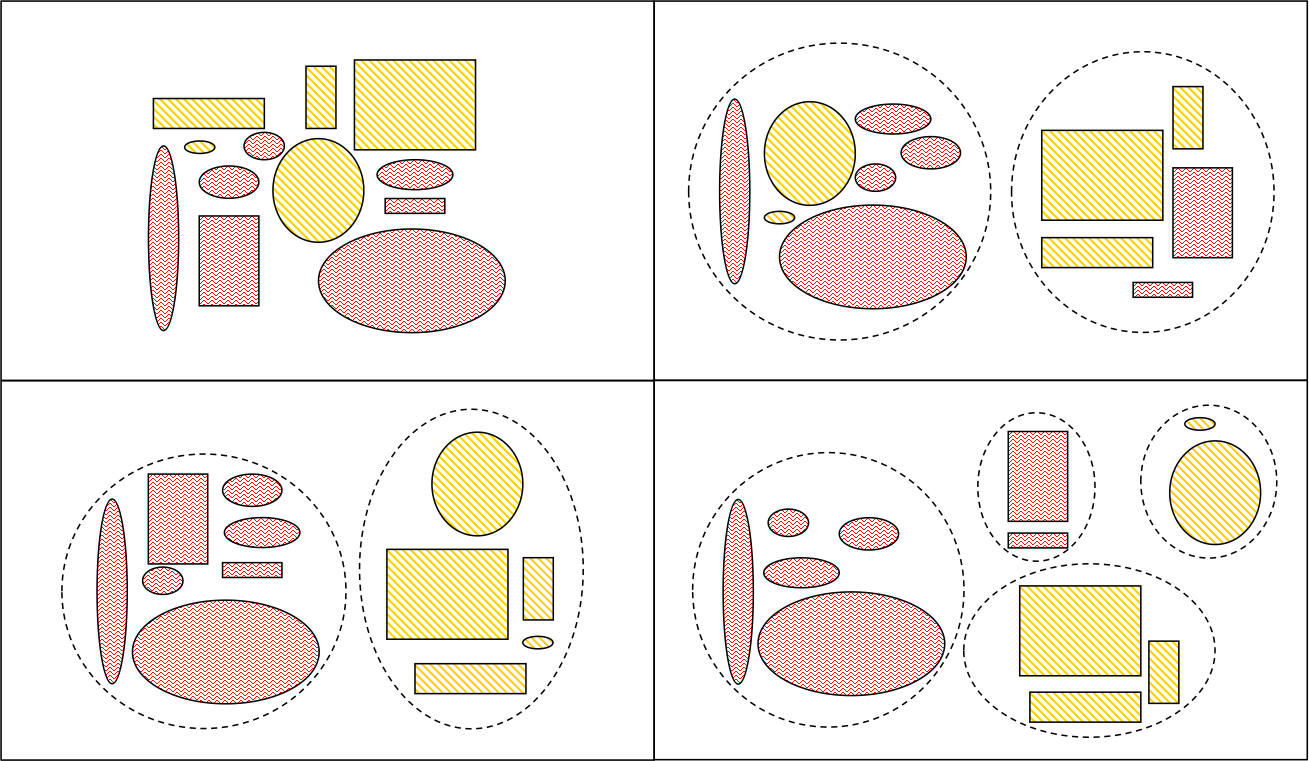
\includegraphics[width=0.7\textwidth]{img/exemplos-agrupamentos}
	\caption{Exemplos de possíveis agrupamentos de um conjunto de objetos}
	\label{fig:exemplos-agrupamentos}
\end{figure}

Uma aplicação típica das técnicas de agrupamento é a identificação de perfis similares de consumidores. Por exemplo, pode ser útil determinar consumidores com gostos em comum no serviço \textit{Netflix}. Ao agrupar os usuários de acordo com seus gostos, é possível direcionar a apresentação de novos títulos em função dessa informação. Se em um grupo de usuários com gostos similares, metade deles avaliou bem um determinado título, seria interessante apresentar este título aos usuários que ainda não assistiram, pois a probabilidade de aceitação é alta. Um segundo exemplo acontece nos mecanismos de busca da Internet. Dado o histórico de visitas de um usuário, quando ele realiza uma nova pesquisa, o motor de busca agrupa os resultados pela similaridade com seu histórico, apresentando assim resultados que com maior probabilidade interesse ao usuário.

Existem diferentes estratégias para agrupamento, como abordagens baseadas em proximidade, probabilísticas ou baseadas em hierarquia. Este capítulo apresenta dois algoritmos de agrupamento, um hierárquico e outro particional. O \textbf{algoritmo hierárquico aglomerativo} é um método que cria diferentes grupos de dados em uma estrutura de hierarquia, que pode ser decomposta conforme a hierarquia desejada. O algoritmo \textbf{$K$-Means} (ou $K$-Médias) é um método particional baseado na proximidade dos dados que utiliza um conjunto de centroides para definir cada grupo.

Ambos os métodos exigem a definição das métricas de similaridade entre dois indivíduos do conjunto de dados. Conforme apresentado no Capítulo~\ref{cap:aprendizado-supervisionado}, uma métrica muito comum é a distância Euclidiana. Seja $x_i$ o valor do atributo $i$ do objeto $x$ e $d$ o número de atributos do objeto, a distância entre dois objetos $a$ e $b$ pode ser definida como:

$$
d(a, b) = \sqrt{\sum_{i=1}^{d} (a_i - b_i)^2}
$$

Para atributos qualitativos, podemos definir que a distância entre dois objetos $a$ e $b$ em função do atributo $i$ (portanto $a_i - b_i$) é 1, caso $a_i \neq b_i$ e 0, caso $a_i = b_i$. Com isso, podemos calcular a distância total em função de todos os $d$ atributos qualitativos como:

$$
d(a, b) = \sum_{i=1}^{d} (a_i - b_i)
$$

Com isso, se um conjunto de dados possui tanto atributos quantitativos quanto qualitativos, devemos calcular as duas distâncias (utilizando os dois conjuntos de atributos) e somá-las para obter a distância final. As seções seguintes apresentam em detalhes o agrupamento de dados utilizando estas métricas de distância.

\section{Agrupamento particional}

Os métodos particionais de agrupamento criam um conjunto de \textit{clusters} (grupos) iniciais e, iterativamente, movem elementos de um \textit{cluster} a outro a fim de melhorar o valor do critério de agrupamento. O número de \textit{clusters} é um parâmetro fixo do algoritmo e um critério comum de agrupamento é a distância entre cada elemento e o centroide do \textit{cluster} ao qual pertence.

\subsection{Algoritmo de \textit{K}-Means}

O principal método de agrupamento particional é o $K$-Means (ou $K$-Médias), que é também um dos algoritmos de agrupamento mais simples e conhecidos. Seu pseudocódigo é apresentado no Algoritmo~\ref{alg:k-means}. O algoritmo escolhe aleatoriamente $k$ objetos do conjunto de dados para formarem os centroides dos $k$ \textit{clusters} que serão construídos. Iterativamente, para cada objeto calcula-se a distância para cada um dos $k$ centroides. O objeto é alocado ao \textit{cluster} cujo centroide está mais próximo. Quando todos os objetos foram alocados, os centroides são recalculados. Na iteração seguinte, os centroides já foram recalculados e alguns objetos passam a estar mais próximo de outro centroide. Neste caso, estes objetos são realocados e os centroides são recalculados. O algoritmo termina quando não existe mais movimentação de objetos de um centroide a outro. Ao final, cada objeto pertence a um dos $k$ \textit{clusters}.

\begin{algorithm}[h]
	\DontPrintSemicolon
	\Entrada{\textit{conjunto de dados -- $X$, número de clusters $k$}}
	\Saida{\textit{partição de $X$ em $k$ clusters}}
	
	\Inicio{
		Escolhe aleatoriamente $k$ elementos de $X$ para formarem os centroides dos \textit{clusters}\;
		
		\Repita{não haverem mais objetos a serem alterados de cluster}{
			\Para{cada objeto $x_i \in X$}{
				\Para{cada cluster $C_j, j = 1, \hdots, k$}{
					Calcula distância entre o objeto $x$ e o centroide $\overline{c}_j$ do cluster $C_j$\;
				}
				Associa $x_i$ ao \textit{cluster} com centroide mais próximo\;
			}
			
			\Para{cada cluster $C_j, j = 1, \hdots, k$}{
				Recalcula o centroide\;
			}
		}
	}
	
	\caption{Pseudocódigo para o algoritmo $K$-Means}
	\label{alg:k-means}
\end{algorithm}

O cálculo do centroide é bastante simples: para cada atributo, o centroide apresenta o valor médio do atributo nos objetos pertencente a ele. No caso de atributos qualitativos, o centroide apresenta a moda observada nos objetos pertencentes a ele. Pelo fato do algoritmo se basear na distância entre os objetos e os centroides, os \textit{clusters} formados são compactos e possuem formato esférico.

Entre as limitações do $K$-Means, destacam-se o fato de não se ajustar a \textit{clusters} com formatos irregulares e a necessidade do usuário informar o número de \textit{clusters}. Para muitos problemas, não se conhece o valor adequado de $k$, o que influencia diretamente na qualidade do agrupamento. Existem algumas variantes deste algoritmo que buscam minimizar estes problemas. A principal vantagem deste algoritmo é sua baixa complexidade -- $O(n)$ -- uma vez que o número de iterações é tipicamente pequeno, $k << n$ e $d << n$.

\begin{figure}[h]
	\centering
	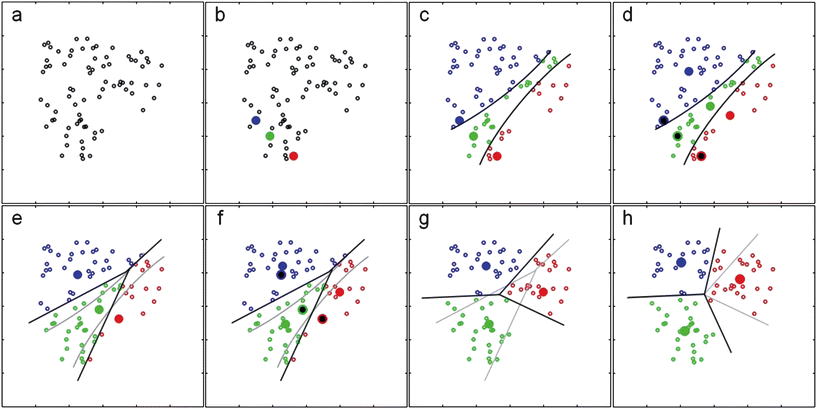
\includegraphics[width=\textwidth]{img/funcionamento-k-means}
	\caption{Funcionamento do algoritmo $K$-Means}
	\label{fig:funcionamento-k-means}
\end{figure}

A Figura~\ref{fig:funcionamento-k-means} apresenta o funcionamento do $K$-Means para um conjunto de dados de duas dimensões. No passo \texttt{(a)} são apresentados os dados, posicionados em função dos valores dos seus dois atributos. No passo \texttt{(b)} são escolhidos três pontos como os centroides (nas cores azul, verde e vermelho), portanto $k = 3$ (existem 3 \textit{clusters}). Os elementos são alocados aos \textit{clusters} no passo \texttt{(c)}. No passo \texttt{(d)}, os centroides são recalculados em função dos elementos dos seu \textit{cluster}. Com isso, os elementos são realocados no passo \texttt{(e)}. O processo se repete nos passos seguintes até a convergência. A figura ainda apresenta as fronteiras que dividem cada \textit{cluster}, conforme a posição dos seus centroides.

\subsection{Exemplo -- agrupamento particional de alunos}
\label{sec:exemplo-k-means}

Vamos considerar um conjunto de dados contendo as notas obtidas por cinco alunos ($A_1, \hdots, A_5$) nas disciplinas de português e matemática. A Tabela~\ref{tab:dados-notas-alunos} apresenta os valores para este conjunto de dados. A Figura~\ref{fig:dados-notas-alunos} apresenta uma representação gráfica destes dados.

\begin{table}[h]
	\centering
	
	\begin{tabular}{lrr}
		\hline
		\textbf{Aluno} & \textbf{Português} & \textbf{Matemática} \\
		\hline
		$A_1$ & 7,0 & 6,5 \\
		$A_2$ & 2,0 & 3,0 \\
		$A_3$ & 7,0 & 5,0 \\
		$A_4$ & 9,5 & 8,0 \\
		$A_5$ & 3,0 & 2,0 \\
		\hline
	\end{tabular}
	
	\caption{Conjunto de dados das notas dos alunos}
	\label{tab:dados-notas-alunos}
\end{table}

\begin{figure}[h]
	\centering
	\pgfplotsset{cycle list={black}}
	
	\begin{tikzpicture}
		\begin{axis}[
			grid=both,
			xmin=0, xmax=10,
			ymin=0, ymax=10,
			minor tick num = 1,
			nodes near coords,
			xlabel=português,
			ylabel=matemática
		]
		
			\addplot+[only marks, point meta=explicit symbolic, mark=o]
				coordinates {
				(7, 6.5) [$A_1$]
				(2, 3) [$A_2$]
				(7, 5) [$A_3$]
				(9.5, 8) [$A_4$]
				(3, 2) [$A_5$]
			};
		\end{axis}
	\end{tikzpicture}
	
	\caption{Representação gráfica das notas dos alunos}
	\label{fig:dados-notas-alunos}
\end{figure}

O primeiro passo consiste em definir o número de \textit{clusters} desejado $k$. Para este exemplo, consideremos $k = 2$. Com isso, definimos aleatoriamente dois elementos para servirem de centroides iniciais. Consideremos os elementos $A_1$ e $A_3$ como centroides e, portanto, $\overline{c}_1 = (7,0; 6,5)$ e $\overline{c}_2 = (7,0; 5,0)$. A Figura~\ref{fig:dados-notas-alunos-centroides-iniciais} apresenta os dados com os centroides posicionados em $A_1$ e $A_3$.

\begin{figure}[h]
	\centering
	\pgfplotsset{cycle list={black\\red\\blue\\}}
	
	
	\begin{tikzpicture}
	\begin{axis}[
		grid=both,
		xmin=0, xmax=10,
		ymin=0, ymax=10,
		minor tick num = 1,
		nodes near coords,
		xlabel=português,
		ylabel=matemática
	]
	
	\addplot+[only marks, point meta=explicit symbolic, mark=*]
		coordinates {
			(2, 3) [$A_2$]
			(9.5, 8) [$A_4$]
			(3, 2) [$A_5$]
		};
		
	\addplot+[only marks, point meta=explicit symbolic, mark=x]
		coordinates {
			(7, 6.5) [$A_1$/$\overline{c}_1$]
		};
	
	\addplot+[only marks, point meta=explicit symbolic, mark=x]
		coordinates {
			(7, 5) [$A_3$/$\overline{c}_2$]
		};
	\end{axis}
	\end{tikzpicture}
	
	\caption{Representação gráfica das notas dos alunos com centroides iniciais}
	\label{fig:dados-notas-alunos-centroides-iniciais}
\end{figure}

O passo seguinte é calcular as distâncias de cada ponto para cada centroide. A métrica adotada é a distância euclidiana. Logo, podemos calcular a distância entre o ponto $A_2$ e o centroide $\overline{c}_1$ como:

\begin{align*}
d(A_2, \overline{c}_1) &= \sqrt{\sum_{i=1}^{d} ({A_2}_i - {\overline{c}_1}_i)^2} \\[10pt]
&= \sqrt{(2,0 - 7,0)^2 + (3,0 - 6,5)^2} \\[10pt]
&= \sqrt{(-5,0)^2 + (-3,5)^2} \\[10pt]
&= \sqrt{25 + 12,25} \\[10pt]
&= \sqrt{37,25} \\[10pt]
&= 6,1
\end{align*}

A matriz de distâncias entre cada elemento e cada centroide é:

\insertspace

\begin{center}
	\begin{tabular}{cccccccc}
		& & $A_1$ & $A_2$ & $A_3$ & $A_4$ & $A_5$ & \\
		$\overline{c}_1$ & \multirow{2}{*}{$\Bigg[$} & 0,0  & 6,1  & 1,5  & 2,9  & 6,0  & \multirow{2}{*}{$\Bigg]$} \\
		\multicolumn{1}{l}{$\overline{c}_2$} & & 1,5  & 5,4  & 0,0  & 3,9  & 5,0  &                  
	\end{tabular}
\end{center}

\insertspace

Com base na matriz de distâncias, atribuímos cada elemento a um dos \textit{clusters}. Caso ele esteja mais próximo do centroide $\overline{c}_1$, ele é alocado ao primeiro \textit{cluster}. Caso ele esteja mais próximo do centroide $\overline{c}_2$, ele é alocado ao segundo \textit{cluster}. A alocação resultante é (matriz de alocação):

\insertspace

\begin{center}
	\begin{tabular}{cccccccc}
		& & $A_1$ & $A_2$ & $A_3$ & $A_4$ & $A_5$ & \\
		$\overline{c}_1$ & \multirow{2}{*}{$\Bigg[$} & 1  & 0  & 0  & 1  & 0  & \multirow{2}{*}{$\Bigg]$} \\
		\multicolumn{1}{l}{$\overline{c}_2$} & & 0  & 1  & 1  & 0  & 1  &                  
	\end{tabular}
\end{center}

\insertspace

A Figura~\ref{fig:dados-notas-alunos-primeira-alocacao} apresenta os elementos alocados a cada cluster, conforme a matriz de alocação apresentada. É possível perceber que a alocação segue a proximidade de cada elemento aos centroides.

\begin{figure}[h]
	\centering
	\pgfplotsset{cycle list={red\\blue\\}}
	
	
	\begin{tikzpicture}
	\begin{axis}[
	grid=both,
	xmin=0, xmax=10,
	ymin=0, ymax=10,
	minor tick num = 1,
	nodes near coords,
	xlabel=português,
	ylabel=matemática
	]
	
	\addplot+[only marks, point meta=explicit symbolic, mark=triangle*]
	coordinates {
		(7, 6.5) [$A_1$/$\overline{c}_1$]
		(9.5, 8) [$A_4$]
	};
	
	\addplot+[only marks, point meta=explicit symbolic, mark=square*]
	coordinates {
		(7, 5) [$A_3$/$\overline{c}_2$]
		(2, 3) [$A_2$]
		(3, 2) [$A_5$]
	};
	\end{axis}
	\end{tikzpicture}
	
	\caption{Representação gráfica das notas dos alunos com alocação inicial}
	\label{fig:dados-notas-alunos-primeira-alocacao}
\end{figure}

O próximo passo consiste em recalcular os centroides em função dos elementos alocados a cada \textit{cluster}. O centroide será posicionado no valor médio dos atributos dos elementos. Como temos dois atributos, recalculamos os centroides como:

\begin{align*}
{\overline{c}_1}_1 &= ({A_1}_1 + {A_4}_1)/2 = (7,0 + 9,5)/2 = 8,25 \\
{\overline{c}_1}_2 &= ({A_1}_2 + {A_4}_2)/2 = (6,5 + 8,0)/2 = 7,25 \\
{\overline{c}_2}_1 &= ({A_2}_1 + {A_3}_1 + {A_5}_1)/3 = (2,0 + 7,0 + 3,0)/3 = 4,0 \\
{\overline{c}_2}_2 &= ({A_2}_2 + {A_3}_2 + {A_5}_2)/3 = (3,0 + 5,0 + 2,0)/3 = 3,3
\end{align*}

Logo, $\overline{c}_1 = (8,25; 7,25)$ e $\overline{c}_2 = (4,0; 3,3)$. A Figura~\ref{fig:dados-notas-alunos-novos-centroides} apresenta o conjunto de dados com os novos centroides (os centroides estão apresentados com o símbolo $\times$). Perceba que os centroides são posicionados no valor médio dos elementos do \textit{cluster}.

\begin{figure}[h]
	\centering
	\pgfplotsset{cycle list={red\\blue\\red\\blue\\}}
	
	
	\begin{tikzpicture}
	\begin{axis}[
	grid=both,
	xmin=0, xmax=10,
	ymin=0, ymax=10,
	minor tick num = 1,
	nodes near coords,
	xlabel=português,
	ylabel=matemática
	]
	
	\addplot+[only marks, point meta=explicit symbolic, mark=x]
		coordinates {
			(8.25, 7.25) [$\overline{c}_1$]
		};
	
	\addplot+[only marks, point meta=explicit symbolic, mark=x]
		coordinates {
			(4, 3.3) [$\overline{c}_2$]
		};
	
	\addplot+[only marks, point meta=explicit symbolic, mark=triangle*]
		coordinates {
			(7, 6.5) [$A_1$]
			(9.5, 8) [$A_4$]
		};
	
	\addplot+[only marks, point meta=explicit symbolic, mark=square*]
		coordinates {
			(7, 5) [$A_3$]
			(2, 3) [$A_2$]
			(3, 2) [$A_5$]
		};
	\end{axis}
	\end{tikzpicture}
	
	\caption{Representação gráfica das notas dos alunos com novos centroides}
	\label{fig:dados-notas-alunos-novos-centroides}
\end{figure}

Com novos centroides, o próximo passo consiste em calcular as novas distâncias entre cada elemento e cada centroide. A matriz de distâncias resultante é apresentada abaixo.

\insertspace

\begin{center}
	\begin{tabular}{cccccccc}
		& & $A_1$ & $A_2$ & $A_3$ & $A_4$ & $A_5$ & \\
		$\overline{c}_1$ & \multirow{2}{*}{$\Bigg[$} & 1,5 & 7,6 & 2,6 & 1,5 & 7,4 & \multirow{2}{*}{$\Bigg]$} \\
		\multicolumn{1}{l}{$\overline{c}_2$} & & 4,4 & 2,0 & 3,4 & 7,2 & 1,6 & 
	\end{tabular}
\end{center}

\insertspace

Perceba que o elemento $A_3$, que antes pertencia ao \textit{cluster} $\overline{c}_2$, possui menor distância ao novo centroide $\overline{c}_1$. Logo, ele será realocado para este \textit{cluster}. A realocação é apresentada na matriz de alocação abaixo e a nova distribuição é apresentada na Figura~\ref{fig:dados-notas-alunos-nova-alocacao}.

\insertspace

\begin{center}
	\begin{tabular}{cccccccc}
		& & $A_1$ & $A_2$ & $A_3$ & $A_4$ & $A_5$ & \\
		$\overline{c}_1$ & \multirow{2}{*}{$\Bigg[$} & 1 & 0 & 1 & 1 & 0 & \multirow{2}{*}{$\Bigg]$} \\
		\multicolumn{1}{l}{$\overline{c}_2$} & & 0 & 1 & 0 & 0 & 1 & 
	\end{tabular}
\end{center}

\insertspace

\begin{figure}[h]
	\centering
	\pgfplotsset{cycle list={red\\blue\\red\\blue\\}}
	
	
	\begin{tikzpicture}
	\begin{axis}[
	grid=both,
	xmin=0, xmax=10,
	ymin=0, ymax=10,
	minor tick num = 1,
	nodes near coords,
	xlabel=português,
	ylabel=matemática
	]
	
	\addplot+[only marks, point meta=explicit symbolic, mark=x]
		coordinates {
			(8.25, 7.25) [$\overline{c}_1$]
		};
	
	\addplot+[only marks, point meta=explicit symbolic, mark=x]
		coordinates {
			(4, 3.3) [$\overline{c}_2$]
		};
	
	\addplot+[only marks, point meta=explicit symbolic, mark=triangle*]
		coordinates {
			(7, 6.5) [$A_1$]
			(7, 5) [$A_3$]
			(9.5, 8) [$A_4$]
		};
	
	\addplot+[only marks, point meta=explicit symbolic, mark=square*]
		coordinates {
			(2, 3) [$A_2$]
			(3, 2) [$A_5$]
		};
	\end{axis}
	\end{tikzpicture}
	
	\caption{Representação gráfica das notas dos alunos com a nova alocação}
	\label{fig:dados-notas-alunos-nova-alocacao}
\end{figure}

Como houveram mudanças de elementos entre os \textit{clusters}, os centroides devem ser recalculados. Os novos centroides são definidos por:

\begin{align*}
	{\overline{c}_1}_1 &= ({A_1}_1 + {A_3}_1 + {A_4}_1)/2 = (7,0 + 7,0 + 9,5)/3 = 7,8 \\
	{\overline{c}_1}_2 &= ({A_1}_2 + {A_3}_2 + {A_4}_2)/2 = (6,5 + 5,0 + 8,0)/3 = 6,5 \\
	{\overline{c}_2}_1 &= ({A_2}_1 + {A_5}_1)/3 = (2,0 + 3,0)/2 = 2,5 \\
	{\overline{c}_2}_2 &= ({A_2}_2 + {A_5}_2)/3 = (3,0 + 2,0)/2 = 2,5
\end{align*}

Os novos centroides são, portanto, $\overline{c}_1 = (7,8; 6,5)$ e $\overline{c}_2 = (2,5; 2,5)$. A Figura~\ref{fig:dados-notas-alunos-novos-centroides-2} apresenta os dados com os novos centroides. Novamente, os centroides são ajustados conforme a proximidade com os novos elementos dos \textit{clusters}.

\begin{figure}[h]
	\centering
	\pgfplotsset{cycle list={red\\blue\\red\\blue\\}}
	
	
	\begin{tikzpicture}
	\begin{axis}[
	grid=both,
	xmin=0, xmax=10,
	ymin=0, ymax=10,
	minor tick num = 1,
	nodes near coords,
	xlabel=português,
	ylabel=matemática
	]
	
	\addplot+[only marks, point meta=explicit symbolic, mark=x]
		coordinates {
			(7.8, 6.5) [$\overline{c}_1$]
		};
	
	\addplot+[only marks, point meta=explicit symbolic, mark=x]
		coordinates {
			(2.5, 2.5) [$\overline{c}_2$]
		};
	
	\addplot+[only marks, point meta=explicit symbolic, mark=triangle*]
		coordinates {
			(7, 6.5) [$A_1$]
			(7, 5) [$A_3$]
			(9.5, 8) [$A_4$]
		};
	
	\addplot+[only marks, point meta=explicit symbolic, mark=square*]
		coordinates {
			(2, 3) [$A_2$]
			(3, 2) [$A_5$]
		};
	\end{axis}
	\end{tikzpicture}
	
	\caption{Representação gráfica das notas dos alunos com novos centroides -- 2}
	\label{fig:dados-notas-alunos-novos-centroides-2}
\end{figure}

O próximo passo consiste em recalcular as distâncias entre cada elemento e cada novo centroide. A matriz de distâncias é dada por:

\insertspace

\begin{center}
	\begin{tabular}{cccccccc}
		& & $A_1$ & $A_2$ & $A_3$ & $A_4$ & $A_5$ & \\
		$\overline{c}_1$ & \multirow{2}{*}{$\Bigg[$} & 0,8 & 6,8 & 1,7 & 2,3 & 6,6 & \multirow{2}{*}{$\Bigg]$} \\
		\multicolumn{1}{l}{$\overline{c}_2$} & & 6,0 & 0,7 & 5,1 & 8,9 & 0,7 & 
	\end{tabular}
\end{center}

\insertspace

Com isso, a distribuição dos elementos aos \textit{cluster} fica a seguinte:

\insertspace

\begin{center}
	\begin{tabular}{cccccccc}
		& & $A_1$ & $A_2$ & $A_3$ & $A_4$ & $A_5$ & \\
		$\overline{c}_1$ & \multirow{2}{*}{$\Bigg[$} & 1 & 0 & 1 & 1 & 0 & \multirow{2}{*}{$\Bigg]$} \\
		\multicolumn{1}{l}{$\overline{c}_2$} & & 0 & 1 & 0 & 0 & 1 & 
	\end{tabular}
\end{center}

\insertspace

Como nenhum elemento trocou de \textit{cluster}, os centroides permanecem os mesmos e o algoritmo termina. Logo, o agrupamento final é aquele apresentado na Figura~\ref{fig:dados-notas-alunos-novos-centroides-2}. O primeiro \textit{cluster} é composto pelos elementos $\{A_1, A_3, A_4\}$, enquanto o segundo \textit{cluster} é composto pelos elementos $\{A_2, A_5\}$.

\section{Agrupamento hierárquico}

Os métodos de agrupamento hierárquicos também se baseiam na proximidade dos dados para execução da tarefa. Eles criam uma sequência de partições aninhadas, iniciando com cada elemento em um \textit{cluster} único e, iterativamente, une dois \textit{clusters} até formar um grande \textit{cluster} único. Cada partição intermediária é mantida e pode ser recuperada.

\subsection{Método aglomerativo}

O método aglomerativo é o algoritmo hierárquico de agrupamento mais utilizado. Seu pseudocódigo é apresentado no Algoritmo~\ref{alg:metodo-aglomerativo}. Considerando o tamanho do conjunto de dados $|X| = n$, criamos $n$ \textit{clusters}, cada um com um único elemento. A cada iteração, selecionamos os dois \textit{clusters} mais próximos e combinamos em um \textit{cluster} único. O algoritmo termina quando todos os elementos pertencem ao mesmo \textit{cluster}.

\begin{algorithm}[h]
	\DontPrintSemicolon
	\Entrada{\textit{conjunto de dados -- $X$}}
	\Saida{\textit{hierarquia de partições de $X$}}
	
	\Inicio{
		Criar $|X|$ \textit{clusters} e alocar cada objeto a um \textit{cluster}\;
		\Enqto{há clusters para agrupar}{
			Calcular matriz de distâncias entre os pares de \textit{clusters} disponíveis, utilizando uma \textit{\underline{métrica de integração}}\;
			Combinar o par de \textit{clusters} $c_i$ e $c_j$ mais próximo, gerando um único \textit{cluster} $c_{ij}$\;
		}
	}
	
	\caption{Pseudocódigo para o método aglomerativo de agrupamento hierárquico}
	\label{alg:metodo-aglomerativo}
\end{algorithm}

O resultado do método aglomerativo é toda a sequência de \textit{clusters} gerada durante a execução do algoritmo. Esta sequência pode ser analisada na forma de um dendrograma, como mostra a Figura~\ref{fig:exemplo-dendrograma}. O início do algoritmo apresenta todos os elementos separados em $n$ \textit{clusters} (base da imagem da esquerda). Na primeira iteração, os \textit{clusters} dos elementos $D$ e $E$ são combinados. Na segunda iteração, o \textit{cluster} $\{D, E\}$ é combinado com o \textit{cluster} do elemento $C$. Na terceira iteração, os \textit{clusters} dos elementos $A$ e $B$ são combinados. A execução segue até que todos os elementos estejam combinados em um elemento único. As uniões do dendrograma mostram a hierarquia dos \textit{clusters}, quanto mais acima, mais geral é o \textit{cluster}.

\begin{figure}[h]
	\centering
	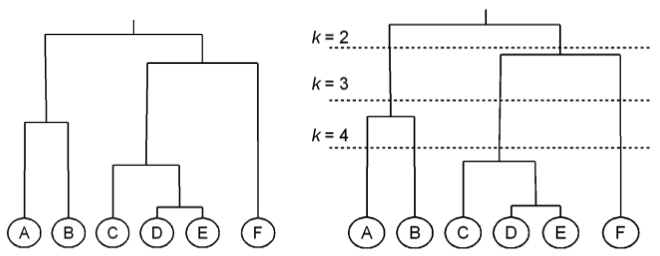
\includegraphics[width=\textwidth]{img/exemplo-dendrograma}
	\caption{Exemplo de dendrograma resultante do método aglomerativo}
	\label{fig:exemplo-dendrograma}
\end{figure}

Dada a hierarquia gerada, é possível recuperar o número desejado de \textit{clusters}. Isso é apresentado na imagem da direita da Figura~\ref{fig:exemplo-dendrograma}. Caso queiramos obter 4 \textit{clusters}, é realizado um corte no dendrograma com o número de partições correspondente. Ou seja, é possível recuperar qualquer quantidade de \textit{clusters}. Por exemplo, os \textit{clusters} resultantes para diferentes valores de $k$ são:
\begin{itemize}
	\item $k = 2$: $\{A, B\}$ e $\{C, D, E, F\}$.
	\item $k = 3$: $\{A, B\}$, $\{C, D, E\}$ e $\{F\}$.
	\item $k = 4$: $\{A\}$, $\{B\}$, $\{C, D, E\}$ e $\{F\}$.
\end{itemize}

Para implementar o método aglomerativo, é necessário definir a \textbf{métrica de integração} utilizada para calcular a distância entre diferentes \textit{clusters}. Existem quatro principais abordagens: ligação mínima, ligação máxima, ligação média e centroide. Estas abordagens são ilustradas na Figura~\ref{fig:exemplos-distancias-cluster}.

\begin{figure}[h]
	\centering
	
	\subfigure[]{
		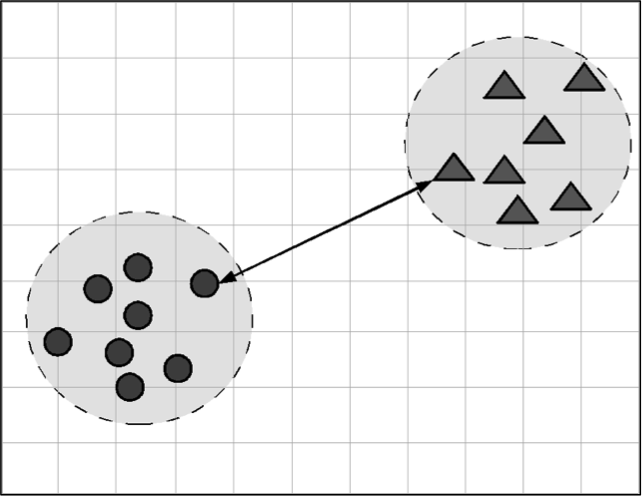
\includegraphics[width=0.4\textwidth]{img/dist-ligacao-minima}
	}
	\subfigure[]{
		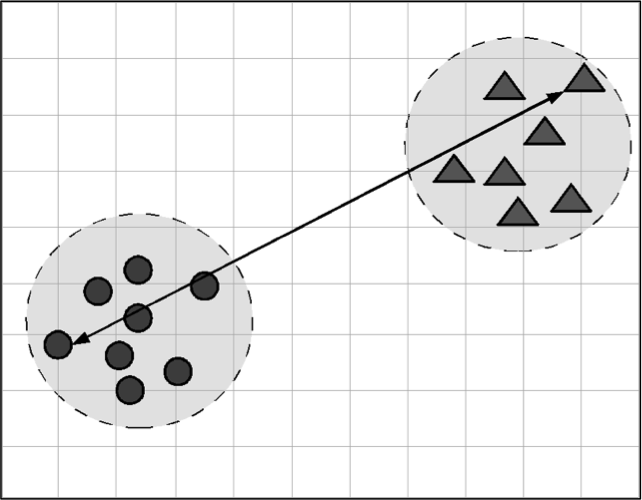
\includegraphics[width=0.4\textwidth]{img/dist-ligacao-maxima}
	}
	\subfigure[]{
		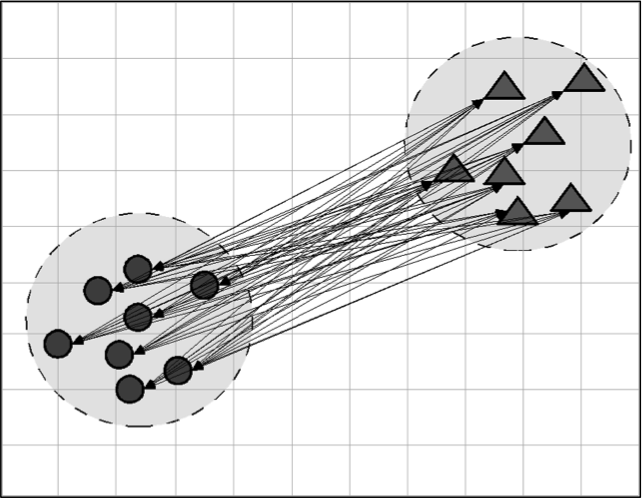
\includegraphics[width=0.4\textwidth]{img/dist-ligacao-media}
	}
	\subfigure[]{
		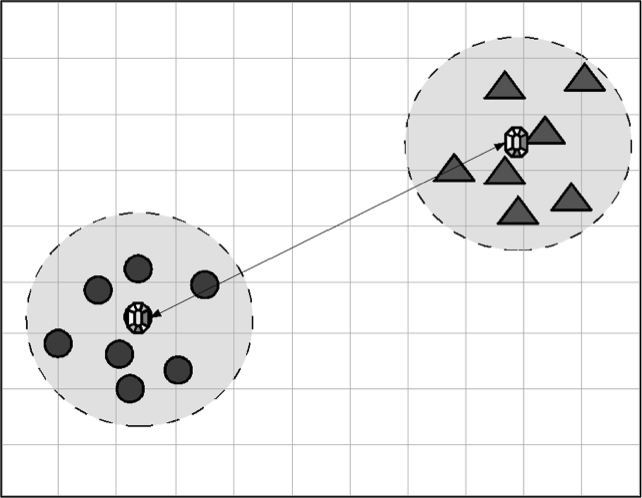
\includegraphics[width=0.4\textwidth]{img/dist-centroide}
	}
	
	\caption{Métricas de integração (distâncias) entre \textit{clusters}}
	\label{fig:exemplos-distancias-cluster}
\end{figure}

A \textbf{ligação mínima} (Figura~\ref{fig:exemplos-distancias-cluster} -- \texttt{a}) utiliza como distância entre dois \textit{clusters} a distância entre o par de elementos mais próximos de ambos. A \textbf{ligação máxima} (Figura~\ref{fig:exemplos-distancias-cluster} -- \texttt{b}) adota a estratégia oposta, utilizando a distância entre o par de elementos mais distantes em ambos os \textit{clusters}. A \textbf{ligação média} (Figura~\ref{fig:exemplos-distancias-cluster} -- \texttt{c}) calcula a distância entre todos os pares de elementos entre os \textit{clusters} e utiliza como média a métrica destes valores. Finalmente, a abordagem por \textbf{centroide} (Figura~\ref{fig:exemplos-distancias-cluster} -- \texttt{d}) calcula o centroide de cada \textit{cluster} e adota como métrica a distância entre eles.

O método aglomerativo é frequentemente utilizado pela sua flexibilidade com relação ao nível de granularidade, pela facilidade de adoção de diferentes métricas para a distância e pela possibilidade de utilizar atributos de diferentes naturezas. No entanto, esta abordagem possui um critério de terminação vago e não retorna para modificar \textit{clusters} já construídos. A complexidade do método é $O(n^2)$.

\subsection{Exemplo -- agrupamento hierárquico de alunos}

Vamos considerar o mesmo conjunto de dados da Seção~\ref{sec:exemplo-k-means}, com as notas obtidas pelos cinco alunos nas disciplinas de português e matemática. A Tabela~\ref{tab:dados-notas-alunos-2} apresenta novamente estes dados. A representação gráfica dos dados é reapresentada na Figura~\ref{fig:dados-notas-alunos-2}.

\begin{table}[h]
	\centering
	
	\begin{tabular}{lrr}
		\hline
		\textbf{Aluno} & \textbf{Português} & \textbf{Matemática} \\
		\hline
		$A_1$ & 7,0 & 6,5 \\
		$A_2$ & 2,0 & 3,0 \\
		$A_3$ & 7,0 & 5,0 \\
		$A_4$ & 9,5 & 8,0 \\
		$A_5$ & 3,0 & 2,0 \\
		\hline
	\end{tabular}
	
	\caption{Conjunto de dados das notas dos alunos}
	\label{tab:dados-notas-alunos-2}
\end{table}

\begin{figure}[h]
	\centering
	\pgfplotsset{cycle list={black}}
	
	\begin{tikzpicture}
	\begin{axis}[
		grid=both,
		xmin=0, xmax=10,
		ymin=0, ymax=10,
		minor tick num = 1,
		nodes near coords,
		xlabel=português,
		ylabel=matemática
	]
	
	\addplot+[only marks, point meta=explicit symbolic, mark=*]
		coordinates {
			(7, 6.5) [$A_1$]
			(2, 3) [$A_2$]
			(7, 5) [$A_3$]
			(9.5, 8) [$A_4$]
			(3, 2) [$A_5$]
		};
	\end{axis}
	\end{tikzpicture}
	
	\caption{Representação gráfica das notas dos alunos}
	\label{fig:dados-notas-alunos-2}
\end{figure}

Cada elemento do conjunto de dados forma um \textit{cluster}. O primeiro passo consiste em calcular a distância entre cada \textit{cluster}. Adotaremos a ligação mínima entre \textit{clusters} como métrica de integração. Com isso, as distâncias são definidas como:

\insertspace

\begin{center}
	\begin{tabular}{cccccc}
		      & $A_1$ & $A_2$ & $A_3$ & $A_4$ & $A_5$ \\
		$A_1$ &   0   &  6,1  &  1,5  &  2,9  &  6,0  \\
		$A_2$ &   -   &   0   &  5,4  &  9,0  &  1,4  \\
		$A_3$ &   -   &   -   &   0   &  2,4  &  5,0  \\
		$A_4$ &   -   &   -   &   -   &   0   &  8,8  \\
		$A_5$ &   -   &   -   &   -   &   -   &   0
	\end{tabular}
\end{center}

\insertspace

Os elementos/\textit{clusters} mais próximos são $A_2$ e $A_5$. Logo, eles são selecionados para formar um único \textit{cluster}. A Figura~\ref{fig:dados-notas-alunos-particao} apresenta o conjunto de dados com a combinação dos elementos $A_2$ e $A_5$ em um único \textit{cluster}.

\begin{figure}[h]
	\centering
	\pgfplotsset{cycle list={black}}
	
	\begin{tikzpicture}
	\begin{axis}[
		grid=both,
		xmin=0, xmax=10,
		ymin=0, ymax=10,
		minor tick num = 1,
		nodes near coords,
		xlabel=português,
		ylabel=matemática
	]
	
	\addplot+[only marks, point meta=explicit symbolic, mark=*]
	coordinates {
		(7, 6.5) [$A_1$]
		(2, 3) [$A_2$]
		(7, 5) [$A_3$]
		(9.5, 8) [$A_4$]
		(3, 2) [$A_5$]
	};
	
	\draw [red] (26,28) ellipse [
		rotate=45,
		x radius=8,
		y radius=16,
	];
	
	\end{axis}
	\end{tikzpicture}
	
	\caption{Representação gráfica das notas dos alunos com a primeira combinação}
	\label{fig:dados-notas-alunos-particao}
\end{figure}

Ao recalcular as distâncias, devemos considerar os quatro \textit{clusters} existentes: $\{A_2, A_5\}$, $A_1$, $A,3$ e $A_4$. No cálculo da distância entre um elemento e o \textit{cluster} $\{A_2, A_5\}$, devemos considerar o elemento do \textit{cluster} mais próximo do segundo elemento (ligação mínima). Observando a Figura~\ref{fig:dados-notas-alunos-particao}, percebemos que os \textit{clusters} mais próximos são $\{A_1\}$ e $\{A_3\}$, que serão recombinados. Os \textit{clusters} da nova iteração são apresentados na Figura~\ref{fig:dados-notas-alunos-particao-2}.

\begin{figure}[h]
	\centering
	\pgfplotsset{cycle list={black}}
	
	\begin{tikzpicture}
	\begin{axis}[
		grid=both,
		xmin=0, xmax=10,
		ymin=0, ymax=10,
		minor tick num = 1,
		nodes near coords,
		xlabel=português,
		ylabel=matemática
	]
	
	\addplot+[only marks, point meta=explicit symbolic, mark=*]
		coordinates {
			(7, 6.5) [$A_1$]
			(2, 3) [$A_2$]
			(7, 5) [$A_3$]
			(9.5, 8) [$A_4$]
			(3, 2) [$A_5$]
		};
	
	\draw [red] (26,28) ellipse [
		rotate=45,
		x radius=8,
		y radius=16,
	];
	
	\draw [blue] (70,60) ellipse [
		rotate=0,
		x radius=8,
		y radius=16,
	];
	
	\end{axis}
	\end{tikzpicture}
	
	\caption{Representação gráfica das notas dos alunos com a segunda combinação}
	\label{fig:dados-notas-alunos-particao-2}
\end{figure}

A próxima iteração seleciona os \textit{clusters} $\{A_1, A_3\}$ e $\{A_4\}$ para combinação, gerando a partição apresentada na Figura~\ref{fig:dados-notas-alunos-particao-3}. Finalmente, os dois \textit{clusters} são combinados, conforme apresentado na Figura~\ref{fig:dados-notas-alunos-particao-4}. O algoritmo finaliza sua execução, pois criou toda a hierarquia de \textit{clusters}.

\begin{figure}[h]
	\centering
	\pgfplotsset{cycle list={black}}
	
	\begin{tikzpicture}
	\begin{axis}[
		grid=both,
		xmin=0, xmax=10,
		ymin=0, ymax=10,
		minor tick num = 1,
		nodes near coords,
		xlabel=português,
		ylabel=matemática
	]
	
	\addplot+[only marks, point meta=explicit symbolic, mark=*]
		coordinates {
			(7, 6.5) [$A_1$]
			(2, 3) [$A_2$]
			(7, 5) [$A_3$]
			(9.5, 8) [$A_4$]
			(3, 2) [$A_5$]
		};
	
	\draw [red] (26,28) ellipse [
		rotate=45,
		x radius=8,
		y radius=16,
	];
	
	\draw [blue] (70,60) ellipse [
		rotate=0,
		x radius=8,
		y radius=16,
	];
	
	\draw [green] (78,68) ellipse [
		rotate=315,
		x radius=16,
		y radius=30,
	];
	
	\end{axis}
	\end{tikzpicture}
	
	\caption{Representação gráfica das notas dos alunos com a terceira combinação}
	\label{fig:dados-notas-alunos-particao-3}
\end{figure}

\begin{figure}[h]
	\centering
	\pgfplotsset{cycle list={black}}
	
	\begin{tikzpicture}
	\begin{axis}[
		grid=both,
		xmin=0, xmax=10,
		ymin=0, ymax=10,
		minor tick num = 1,
		nodes near coords,
		xlabel=português,
		ylabel=matemática
	]
	
	\addplot+[only marks, point meta=explicit symbolic, mark=*]
		coordinates {
			(7, 6.5) [$A_1$]
			(2, 3) [$A_2$]
			(7, 5) [$A_3$]
			(9.5, 8) [$A_4$]
			(3, 2) [$A_5$]
		};
	
	\draw [red] (26,28) ellipse [
		rotate=45,
		x radius=8,
		y radius=16,
	];
	
	\draw [blue] (70,60) ellipse [
		rotate=0,
		x radius=8,
		y radius=16,
	];
	
	\draw [green] (78,68) ellipse [
		rotate=315,
		x radius=16,
		y radius=30,
	];
	
	\draw [brown] (56,55) ellipse [
		rotate=304,
		x radius=25,
		y radius=60,
	];
	
	\end{axis}
	\end{tikzpicture}
	
	\caption{Representação gráfica das notas dos alunos com a quarta combinação}
	\label{fig:dados-notas-alunos-particao-4}
\end{figure}

O resultado do método aglomerativo com as notas dos alunos pode (e deve) ser representado através de um dendrograma. Ele é capaz de apresentar a hierarquia de \textit{clusters} e facilita a recuperação deles conforme o número de \textit{clusters} desejado. A Figura~\ref{fig:dados-notas-alunos-dendrograma} apresenta o dendrograma resultante. Finalmente, podemos obter os \textit{clusters} de acordo com o valor desejado para $k$ (número de \textit{clusters}):
\begin{itemize}
	\item $k = 2$: $\{A_1, A_3, A_4\}$ e $\{A_2, A_5\}$.
	\item $k = 3$: $\{A_1, A_3\}$, $\{A_4\}$ e $\{A_2, A_5\}$.
	\item $k = 4$: $\{A_1\}$, $\{A_3\}$, $\{A_4\}$ e $\{A_2, A_5\}$.
\end{itemize}

\begin{figure}[h!]
	\centering
	
	\begin{tikzpicture}[sloped]
		\node (a1) at (-4,0) {$A_1$};
		\node (a3) at (-2,0) {$A_3$};
		\node (a4) at (0,0) {$A_4$};
		\node (a2) at (2,0) {$A_2$};
		\node (a5) at (4,0) {$A_5$};
		
		\node (a2a5) at (3,1) {};
		\draw (a2) |- (a2a5.center);
		\draw (a5) |- (a2a5.center);
		
		\node (a1a3) at (-3,2) {};
		\draw (a1) |- (a1a3.center);
		\draw (a3) |- (a1a3.center);
		
		\node (a1a3a4) at (-1.5,3) {};
		\draw (a1a3.center) |- (a1a3a4.center);
		\draw (a4) |- (a1a3a4.center);
		
		\node (a1a3a4a2a5) at (0.75,4) {};
		\draw (a1a3a4.center) |- (a1a3a4a2a5.center);
		\draw (a2a5.center) |- (a1a3a4a2a5.center);
		
		\node (top) at (0.75,4.5) {};
		\draw (a1a3a4a2a5.center) |- (top.center);
	\end{tikzpicture}
	
	\caption{Dendrograma do agrupamento hierárquico das notas dos alunos}
	\label{fig:dados-notas-alunos-dendrograma}
\end{figure}

\section{Exercícios}

\resetexercisenumbering

\begin{exercise}
Pesquise aplicações de algoritmos de agrupamento. Destaque as técnicas utilizadas e os resultados obtidos.
\end{exercise}

\begin{exercise}
Pesquise casos onde o algoritmo de $K$-Means não apresenta bons resultados.
\end{exercise}

\begin{exercise}
Pesquise sobre o algoritmo de agrupamento \textit{DBScan}. Como ele funciona quais suas vantagens em relação ao $K$-Means?
\end{exercise}

\begin{exercise}
Dados os três objetos apresentados abaixo (atributos de funcionários), calcule a distância entre cada par de elementos e mostre os dois elementos mais próximos.

\begin{table}[h]
	\centering
	\begin{tabular}{ccccc}
		\hline
		\textbf{Idade} & \textbf{Gênero} & \textbf{Tempo de serviço} & \textbf{Formação} & \textbf{Salário} \\ \hline
		24 & feminino  & 2                &   pós-graduação &         3.200,00         \\ 
		38 & masculino  & 12                &   superior &         4.800,00         \\
		29 & feminino  & 5                &   médio &         2.600,00         \\
		\hline
	\end{tabular}
\end{table}
\end{exercise}

\begin{exercise}
O dendrograma abaixo mostra o agrupamento hierárquico de marcas de veículos. Mostre os elementos de cada grupo, considerando diferentes quantidades de grupos: 2, 3 e 4.

\begin{figure}[h!]
	\centering
	
	\begin{tikzpicture}[sloped]
	\node (a1) at (-4,0) {VW};
	\node (a3) at (-2,0) {GM};
	\node (a4) at (0,0) {Honda};
	\node (a2) at (2,0) {BMW};
	\node (a5) at (4,0) {Audi};
	
	\node (a2a5) at (3,1) {};
	\draw (a2) |- (a2a5.center);
	\draw (a5) |- (a2a5.center);
	
	\node (a1a3) at (-3,2) {};
	\draw (a1) |- (a1a3.center);
	\draw (a3) |- (a1a3.center);
	
	\node (a1a3a4) at (-1.5,3) {};
	\draw (a1a3.center) |- (a1a3a4.center);
	\draw (a4) |- (a1a3a4.center);
	
	\node (a1a3a4a2a5) at (0.75,4) {};
	\draw (a1a3a4.center) |- (a1a3a4a2a5.center);
	\draw (a2a5.center) |- (a1a3a4a2a5.center);
	
	\node (top) at (0.75,4.5) {};
	\draw (a1a3a4a2a5.center) |- (top.center);
	\end{tikzpicture}
\end{figure}
\end{exercise}

\begin{exercise}
Considere parte do conjunto de dados das espécies de íris apresentada abaixo. Mostre a execução do algoritmo $K$-Means com $k = 3$ e apresente os três grupos resultantes. Mostre o resultado final em planos cartesianos para visualização dos elementos, elipses e grupos (o atributo espécie não deve ser utilizado).

\begin{table}[h]
	\centering
	\begin{tabular}{rrrrl}
		\hline
		\textbf{Comp. (P)} & \textbf{Larg. (P)} & \textbf{Comp. (S)} & \textbf{Larg. (S)} & \textbf{Espécie} \\
		\hline
		5,1 & 3,5 & 1,4 & 0,2 & Setosa \\
		4,9 & 3,0 & 1,4 & 0,2 & Setosa \\
		7,0 & 3,2 & 4,7 & 1,4 & Versicolor \\
		6,4 & 3,2 & 4,5 & 1,5 & Versicolor \\
		6,3 & 3,3 & 6,0 & 2,5 & Virgínica \\
		5,8 & 2,7 & 5,1 & 1,9 & Virgínica \\
		\hline
	\end{tabular}
\end{table}
\end{exercise}

\begin{exercise}
Considere os mesmos dados do exercício anterior. Mostre a execução do algoritmo aglomerativo de agrupamento hierárquico e apresente o dendrograma resultante.
\end{exercise}

\begin{exercise}
Considere os dados com as características de esponjas marinhas disponível em \url{https://archive.ics.uci.edu/ml/datasets/Sponge}. Utilize a ferramenta Weka para o agrupamento destes dados. Teste diferentes algoritmos de agrupamento e seus parâmetros. Verifique as métricas de avaliação proporcionadas pela ferramenta e analise o desempenho de cada algoritmo.
\end{exercise}

\begin{exercise}
Considere o mesmo conjunto de dados do exercício anterior. Utilize a biblioteca \textit{JavaML} (ou outra da sua escolha) para execução e avaliação dos algoritmos de agrupamento. Compare o desempenho com aqueles implementados na ferramenta Weka.
\end{exercise}

\begin{exercise}
Implemente o algoritmo de $K$-Means para o conjunto de 100 pontos abaixo. Mostre o valor dos centroides ao final da execução, a disposição dos pontos nos grupos e a representação cartesiana dos resultados.

\begin{table}[h]
	\centering
	\def\arraystretch{1}
	\resizebox{\textwidth}{!}{%
	\begin{tabular}{rr|rr|rr|rr|rr}
		\hline
		\textbf{x} & \textbf{y} & \textbf{x} & \textbf{y} & \textbf{x} & \textbf{y} & \textbf{x} & \textbf{y} & \textbf{x} & \textbf{y} \\ \hline
		2.9986 & 5.4115 	&	7.3792 & 5.6468 	&	2.2180 & 1.7299 	&	6.4154 & 5.4805 	&	8.7612 & 6.4911 	\\
		8.1588 & 4.9327 	&	7.7253 & 6.2002 	&	6.1123 & 5.3547 	&	6.7577 & 5.8193 	&	8.7992 & 6.4291 	\\
		-0.1911 & -1.7320 	&	11.1470 & 7.7087 	&	2.4562 & 3.5604 	&	7.3953 & 5.6697 	&	-1.5520 & -3.9206 	\\
		9.1571 & 6.2303 	&	1.8570 & 2.1072 	&	1.3797 & 0.3961 	&	9.5569 & 7.2170 	&	8.1765 & 6.0644 	\\
		0.8224 & -1.1243 	&	2.9573 & 3.7049 	&	3.2149 & 3.3001 	&	5.9958 & 4.5021 	&	6.8398 & 5.1538 	\\
		0.1308 & -1.8648 	&	0.8489 & 0.2223 	&	9.0940 & 7.0498 	&	8.2078 & 6.2118 	&	0.4978 & 0.4194 	\\
		8.7121 & 6.1395 	&	1.8367 & 1.5076 	&	2.3842 & 2.6039 	&	11.9082 & 7.6112 	&	6.0912 & 4.3148 	\\
		2.2625 & 3.1703 	&	4.7384 & 5.1813 	&	3.3281 & 5.1815 	&	6.0547 & 7.2849 	&	7.3719 & 5.9768 	\\
		1.7972 & 1.7397 	&	1.3665 & 0.6363 	&	8.8959 & 6.4742 	&	8.1267 & 7.0309 	&	8.4350 & 6.3067 	\\
		3.0634 & 3.0133 	&	10.5466 & 6.5951 	&	0.1479 & -0.6412 	&	5.3031 & 4.6593 	&	8.2206 & 6.7469 	\\
		8.1291 & 5.9392 	&	1.6342 & 2.1033 	&	3.0903 & 3.3168 	&	1.4604 & 1.1574 	&	8.2105 & 5.5732 	\\
		10.8097 & 6.8504 	&	6.5543 & 6.2060 	&	0.5014 & -0.0152 	&	10.4773 & 6.5726 	&	8.6842 & 6.3063 	\\
		0.6106 & 0.7215 	&	7.4471 & 6.0770 	&	4.3224 & 5.3156 	&	3.9189 & 4.9542 	&	7.2223 & 5.7820 	\\
		6.1466 & 5.7468 	&	8.0574 & 6.1558 	&	7.1978 & 5.5789 	&	1.1550 & 0.6860 	&	3.0846 & 1.4112 	\\
		6.3625 & 5.1882 	&	8.0896 & 6.3030 	&	7.8588 & 6.7083 	&	0.2094 & -1.9528 	&	6.6620 & 5.3358 	\\
		-1.6208 & -3.8387 	&	1.3350 & 0.4894 	&	9.0953 & 7.3278 	&	7.7698 & 4.9409 	&	4.1014 & 5.9718 	\\
		1.6859 & 1.6659 	&	3.1120 & 3.3676 	&	4.2530 & 5.6024 	&	5.5875 & 5.2593 	&	2.8341 & 4.9589 	\\
		3.8979 & 5.4510 	&	1.0531 & 1.6620 	&	9.4268 & 6.8458 	&	5.7082 & 4.2622 	&	7.8170 & 5.7399 	\\
		1.3537 & 0.7185 	&	1.7550 & 1.7793 	&	2.4428 & 2.1498 	&	2.5005 & 2.8861 	&	7.5139 & 6.1183 	\\
		1.2620 & 1.7233 	&	1.8914 & 0.7850 	&	9.0287 & 6.6842 	&	1.0037 & 0.3312 	&	2.1673 & 3.0574 	\\
		
		\hline
	\end{tabular}
	}
\end{table}
\end{exercise}
\chapter{Aprendizado por reforço}

\framebox[\textwidth]{
	\hspace{1em}
	\vbox{
		\textbf{Leitura obrigatória:}
		\begin{itemize}
			\item \cite{RusselAndNorvig2010} -- Cap. 21 (Aprendizagem por reforço).
			\item \cite{Mitchell1997} -- Cap. 13 (Reinforcement Learning).
		\end{itemize}
		
		\textbf{Leitura complementar:}
		\begin{itemize}
			\item \cite{SuttonAndBarto1998} -- Cap. 1 (Introduction).
			\item \cite{SuttonAndBarto1998} -- Cap. 3 (The Reinforcement Learning Problem).
		\end{itemize}
	}
}

\section{Visão geral}

O aprendizado por reforço tem por objetivo fazer com que um agente aprenda a forma como deve agir para execução de alguma tarefa. O agente aprende a escolher a ação ótima através da sua interação com o ambiente. Por exemplo, um agente pode aprender a movimentar-se em um ambiente físico, organizar volumes em um estoque, ou ainda jogar algum jogo de tabuleiro.

Para isso, o aprendizado por reforço considera que o ambiente (ou um supervisor externo) forneça um retorno ao agente quando ele atinge o objetivo ou quando atinge algum estado de fracasso. O agente recebe uma recompensa (positiva ou negativa) conforme as ações executadas e, com isso, aprende a sequência de ações que maximiza a recompensa. Por exemplo, treinar um agente para jogar damas consiste em dar uma recompensa positiva caso ele ganhe o jogo, uma recompensa negativa caso ele perca o jogo, e nenhuma recompensa nos estágios intermediários. Com isso, o agente aprende a sequência de ações que o levam à vitória e, dessa forma, aprende a jogar damas.

\begin{figure}
	\centering
	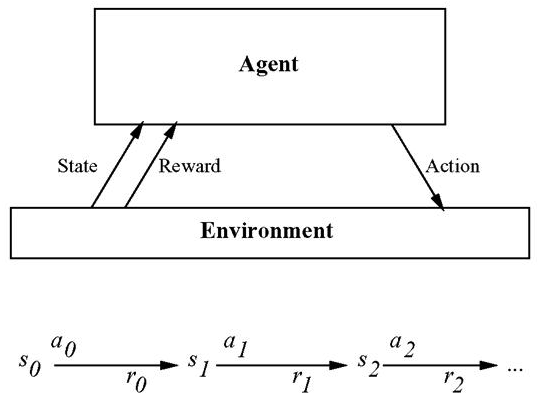
\includegraphics[width=0.5\textwidth]{img/agente-ambiente-recompensa}
	\caption{Interação entre agente e ambiente com recompensa pelas ações}
	\label{fig:agente-ambiente-recompensa}
\end{figure}

A Figura~\ref{fig:agente-ambiente-recompensa} apresenta a ideia geral onde o agente, além de perceber o ambiente e agir sobre ele, recebe uma recompensa em função da ação executada e do resultado obtido por ela. A figura ainda mostra os elementos principais do aprendizado por reforço. Dado um estado $s_0$, o agente executa a ação $a_0$, que modifica o ambiente para o estado $s_1$. Com isso, o agente recebe a recompensa $r_0$. O mesmo ocorre quando, a partir do estado $s_1$, o agente executa a ação $a_1$, levando-o para o estado $s_2$ e recebendo a recompensa $r_1$. Neste sentido, a tarefa do agente é aprender a sequência de ações que maximize as recompensas obtidas. Logo, o aprendizado por reforço torna-se bastante abrangente, podendo ser aplicado a uma variedade de problemas de aprendizagem.

A sequência de ações que o agente deve aprender é chamada de \textbf{política} (ou política de controle). A política é, portanto, uma função que mapeia estados para ações. Podemos denotar a política como $\pi : S \rightarrow A$, que retorna uma ação $a \in A$, dado um estado $s \in S$. Uma notação igualmente comum é $a = \pi(s)$.

O aprendizado por reforço possui algumas características que o difere de outras técnicas de aprendizagem de máquina:

\begin{itemize}
	\item \textbf{Recompensa tardia:} em outras tarefas de aprendizagem de máquina, o agente possui um conjunto de dados de treinamento, sobre o qual deve induzir uma hipótese. No aprendizado por reforço, não existem dados rotulados ou disponíveis \textit{a priori}. O agente deve explorar o conjunto possível de ações e, com o retorno recebido, aprender a política ótima.
	
	\item \textbf{Exploração:} para conhecer as diferentes possibilidades de ações e transições de estados, bem como descobrir qual a melhor sequência de ações, o agente deve explorar o ambiente. Com isso, o agente deve preocupar-se com o equilíbrio entre \textit{explorar} ações desconhecidas, ou \textit{intensificar} sua busca nos melhores caminhos de ações já encontrados (exploração $\times$ intensificação).
	
	\item \textbf{Estados parcialmente observáveis:} muitas vezes o agente não possui a visão completa do seu ambiente. Neste caso, é comum que a melhor ação a se tomar seja aquela que permita uma percepção mais abrangente do seu ambiente. Como exemplo, considere um robô cuja câmera consiga captar apenas parte do entorno.
	
	\item \textbf{Aprendizado de vida longa:} diferente de tarefas de predição de uma função isolada, um agente físico deve aprender atividades periféricas como recarregar sua bateria, movimentar-se para chegar a um ponto específico, etc. Uma vez que o agente pode aprender a partir da exploração do ambiente, não se faz necessária a manutenção de um grande conjunto de dados de teste.
\end{itemize}

\section{Processo de decisão de Markov}

O Processo de Decisão de Markov (MDP -- \textit{Markov Decision Process}) é aplicado quando se deseja tomar uma sequência de decisões, mas o resultado de cada decisão não é claro. O MDP permite, matematicamente, determinar uma política que maximize o retorno esperado da sequência de decisões. Neste sentido, a tarefa de aprendizagem por reforço pode ser modelada como um MDP.

\subsection{Funcionamento}

Em cada instance discreto de tempo $t$, o agente percebe o estado atual $s_t$, escolhe e executa a ação atual $a_t$. O ambiente responde com uma recompensa $r_t = (s_t, a_t)$ e produz o estado sucessor $s_{t+1} = \delta(s_t, a_t)$. As funções $r$ e $\delta$ fazem parte do ambiente e não necessariamente são conhecidas pelo agente\footnote{Em muitos casos, estas funções podem ser implementadas diretamente no agente.}.

Queremos aprender uma política ótima $\pi(s_t) = a_t$ em que dado um estado $s_t$, o agente possa escolher a melhor ação possível $a_t$. A política ótima é aquela que produz a maior recompensa acumulada. Logo, podemos definir a recompensa acumulada como:

\begin{align*}
V^\pi(s_t) &\equiv r_t + \gamma r_{t+1} + \gamma^2 r_{t+2} + \hdots \\[10pt]
&\equiv \sum_{i=0}^{\infty} \gamma^i r_{t+i}
\end{align*}

A constance $0 \le \gamma < 1$ determina o valor relativo entre recompensas a serem recebidas no futuro e a recompensa imediata. Ou seja, uma recompensa recebida $i$ passos a frente é descontada exponencialmente por um fator $\gamma^i$. Se definirmos $\gamma = 0$, somente a recompensa imediata é considerada. Por outro lado, com $\gamma$ próximo a 1 é dada maior ênfase a recompensas futuras em relação à recompensa imediata. Logo, $V^\pi(s)$ pode ser chamada de \textit{recompensa cumulativa descontada} obtida pela política $\pi$ a partir do estado $s$.

Com isso, a tarefa de aprendizado do agente consiste em selecionar a política que maximiza a recompensa cumulativa descontada para todos os estados. Chamamos esta política de \textbf{política ótima} e denotamos por $\pi^*$. A recompensa cumulativa descontada da política ótima $V^{\pi^*}(s)$ pode ser simplificada para $V^*(s)$. Com isso, denotamos a política ótima como:

$$
\pi^* \equiv \argmax_{\pi} V^\pi(s), \forall s
$$

\subsection{Exemplo -- movimentação no ambiente de grade}

Consideremos o ambiente apresentado na Figura~\ref{fig:exemplo-rl-cenario}. Consiste em uma grade em que cada célula representa um possível estado. As setas representam as possíveis ações de movimentação do agente, cujo valor associado corresponde à recompensa da respectiva ação. Perceba que o estado \textbf{G} é o único que atribui uma recompensa diferente de zero às ações que levam a ele. Logo, podemos chamá-lo de \textit{estado objetivo}. Além disso, ele não possui ações que permitam ao agente sair deste estado, o que nos permite chamá-lo de \textit{estado de absorção}. A tarefa, portanto, consiste em determinar a sequência de ações que levam ao estado objetivo pelo menor caminho.

\begin{figure}[h]
	\centering
	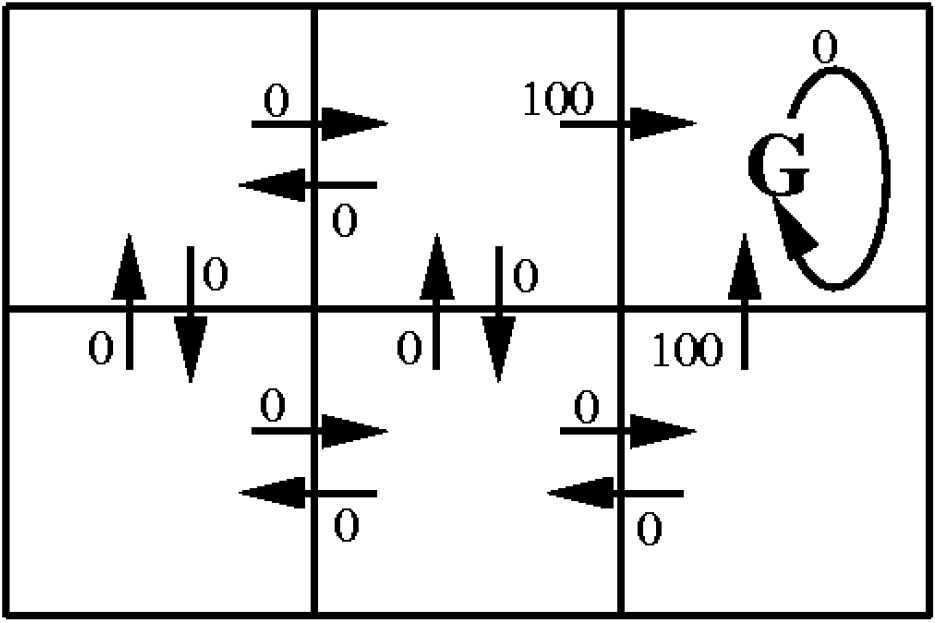
\includegraphics[width=0.3\textwidth]{img/exemplo-rl-cenario}
	\caption{Ambiente em grade cuja tarefa é chegar ao estado G}
	\label{fig:exemplo-rl-cenario}
\end{figure}

Uma vez definidos os estados, ações e recompensas, precisamos definir o valor do desconto $\gamma$ para definir a política ótima $\pi^*$. Consideremos $\gamma = 0.9$. A Figura~\ref{fig:exemplo-rl-politica-otima} mostra uma política ótima (podem existir outras) para este cenário. Esta política move o agente diretamente para o estado objetivo, considerando o menor número de passos possível. Como qualquer política, ela define uma única possível ação a partir de um determinado estado.

\begin{figure}[h]
	\centering
	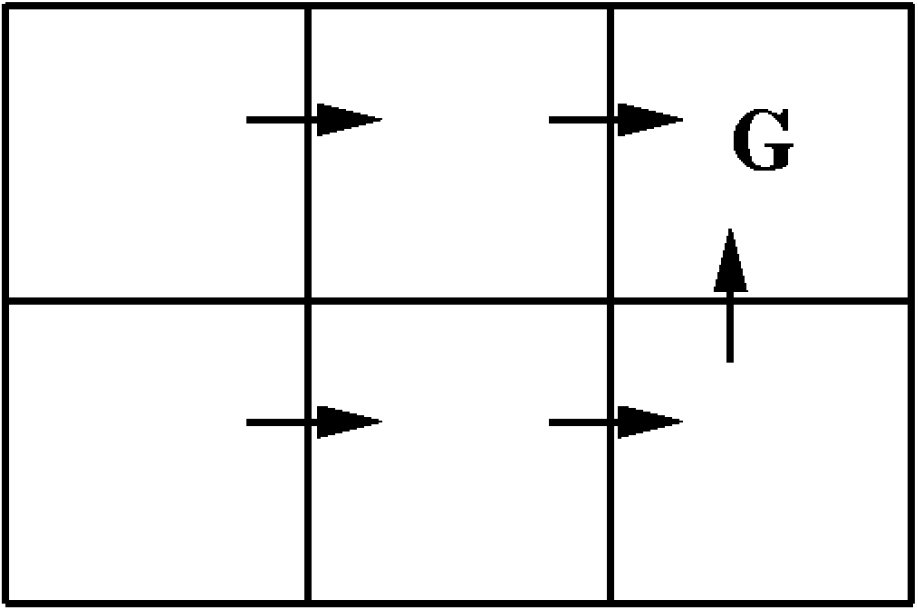
\includegraphics[width=0.3\textwidth]{img/exemplo-rl-politica-otima}
	\caption{Uma política ótima para o ambiente em grade}
	\label{fig:exemplo-rl-politica-otima}
\end{figure}

A Figura~\ref{fig:exemplo-rl-recompensas} mostra o ambiente em grade preenchido com os valores de recompensa $V^*(s)$ para cada estado, considerando o fator de desconto $\gamma = 0.9$. O estado inferior direito possui valor associado de recompensa 100 pois selecionando a ação ``\textit{para cima}'' o agente receberá uma recompensa \textit{imediata} de 100. O mesmo acontece com o estado a esquerda do estado \textbf{G}. Já o estado inferior central possui recompensa de 90, pois a ação ``\textit{para direita}'' não leva a uma recompensa imediata. Logo, a recompensa futura deve ser descontada. Aplicando o fator de desconto $\gamma^1$, pois a recompensa será recebida 1 passo no futuro, associamos a recompensa resultante ($0.9 \times 100 = 90$) a este estado. O mesmo acontece com o estado inferior esquerdo, a recompensa está dois passos a frente, logo utilizamos o fator de desconto $\gamma^2 = 0.81$ e associamos a recompensa $0.81 \times 100 = 81$ a este estado.

\begin{figure}[h]
	\centering
	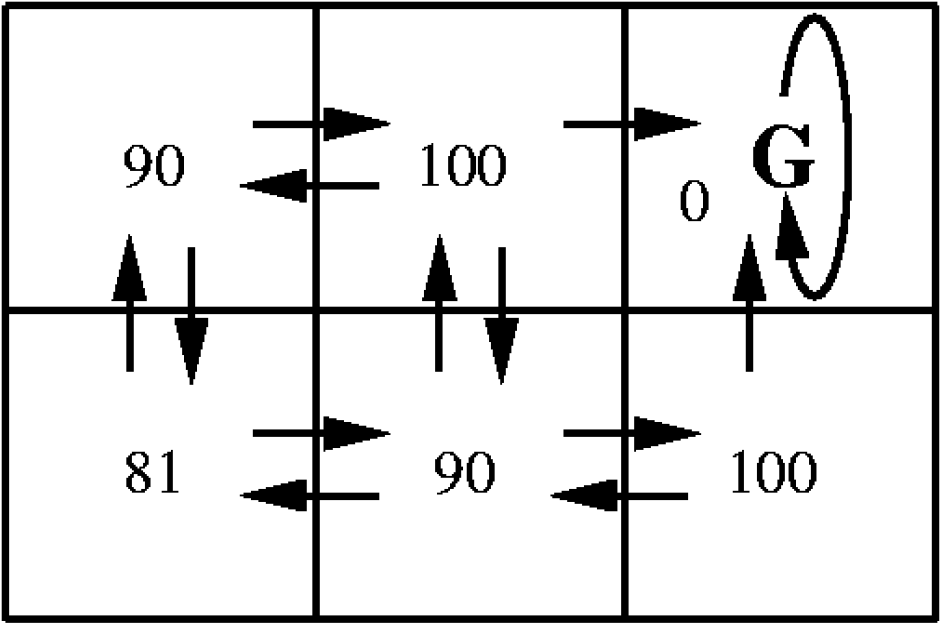
\includegraphics[width=0.3\textwidth]{img/exemplo-rl-recompensas}
	\caption{Valores de recompensa $V^*(s)$ da política ótima para o ambiente em grade}
	\label{fig:exemplo-rl-recompensas}
\end{figure}

\section{Algoritmo de \textit{Q}-Learning}

O algoritmo de $Q$-Learning é a abordagem mais conhecida de aprendizado por reforço. Esta seção mostra seu funcionamento, aplicação e um exemplo.

\subsection{Funcionamento}

O Algoritmo de $Q$-Learning permite ao agente aprender uma política ótima $\pi^*$ para qualquer ambiente arbitrário. A cada estado, o agente deve selecionar a ação $a$ que forneça o maior benefício em termos da recompensa imediata $r(s, a)$ somada à recompensa futura acumulada do próximo estado $V^*(s')$, descontado por $\gamma$. Considerando que o próximo estado é obtido em função da execução da ação $a$ no estado atual $s$, temos $s' = \delta(s, a)$. Com isso, definimos a função $Q$ (que dá nome ao algoritmo), como a maior recompensa acumulada descontada que pode ser obtida a partir do estado $s$, aplicando a ação $a$ como primeira ação.

$$
Q(s, a) = r(s, a) + \gamma V^* (\delta(s, a))
$$

A função $Q$ pode ainda ser vista como a recompensa obtida pela execução de $a$ em $s$, mais a recompensa descontada ao seguir a política ótima após isso. Como o agente seleciona a ação que maximiza $Q(s, a)$, a política ótima é definida por:

$$
\pi^*(s) = \argmax_{a} Q(s, a)
$$

Se o agente conhece as funções $r(s, a)$ e $\delta(s, a)$, isto é, ele possui conhecimento completo do ambiente, ele pode determinar o valor de $Q$ para todas as ações e, com isso, obter a política ótima. A Figura~\ref{fig:exemplo-rl-tabela-q} apresenta o valor de $Q$ para todas as ações possíveis. Perceba que ao selecionar a ação que maximiza $Q$ em cada estado, chegamos ao estado objetivo com o menor número de passos possível.

\begin{figure}[h]
	\centering
	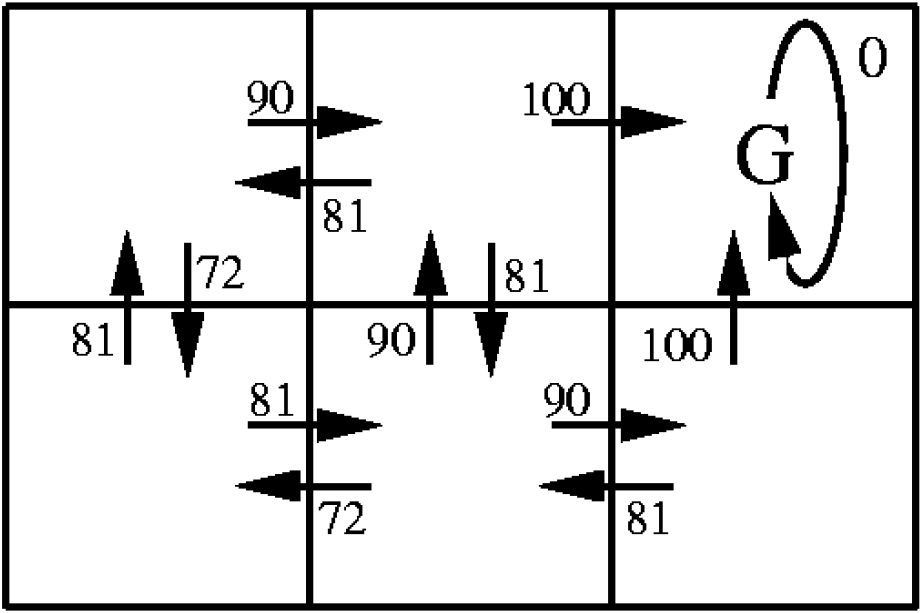
\includegraphics[width=0.3\textwidth]{img/exemplo-rl-tabela-q}
	\caption{Valores de $Q(s, a)$ para o ambiente em grade}
	\label{fig:exemplo-rl-tabela-q}
\end{figure}

É correto afirmar que a recompensa acumulada descontada $V^*(s)$ é igual à maximização da função $Q$, para um dado estado. Ou seja:

$$
V^*(s) = \max_{a'} Q(s, a')
$$

Com isso, podemos reescrever a função $Q$ como uma recursão da seguinte forma:

$$
Q(s, a) = r(s, a) + \gamma \max_{a'} Q(\delta(s, a), a')
$$

O agente deve induzir uma hipótese para a função $Q$. A hipótese induzida é representada por $\widehat{Q}$. O agente representa esta hipótese através de uma grande tabela, contendo o valor associado a cada par \textit{estado-ação}. Ou seja, a entrada $\langle s, a \rangle$ armazena o valor de $\widehat{Q}(s, a)$\footnote{Perceba que não se trata do valor real $Q(s, a)$, mas da indução do agente sobre este valor.}. O agente inicializa esta tabela com zero (ou outros valores aleatórios) e repetidamente observa seu estado atual $s$, seleciona uma ação $a$, executa a ação e observa a recompensa $r = r(s, a)$ e o novo estado $s'= \delta(s, a)$. Após isso, ele atualiza a entrada da tabela $\widehat{Q}(s, a)$ seguindo a regra:

$$
\widehat{Q}(s, a) \gets r + \gamma \max_{a'} \widehat{Q}(s', a')
$$

Perceba que a atualização da tabela utiliza os próprios valores previamente armazenados ($\widehat{Q}$). Com isso, o agente não precisa conhecer as funções $\delta$ e $r$ para aprender, basta repetidamente explorar o ambiente, verificando o estado e a recompensa resultante da ação executada e, com isso, atualizar a tabela $\widehat{Q}$. Portanto, $\widehat{Q}$ pode ser visto como uma aproximação da função real $Q$.

O Algoritmo~\ref{alg:q-learning} apresenta um pseudocódigo para o algoritmo de $Q$-Learning. O primeiro passo consiste em inicializar a tabela $\widehat{Q}$. Após isso, repetidamente o agente percebe seu estado inicial e, enquanto não encontrar o estado objetivo ele seleciona uma ação, a executa, verifica a recompensa imediata e o estado resultante, atualizando a tabela $Q$. Este processo é repetido por um conjunto finito de iterações, chamadas de \textbf{episódios}. A quantidade de episódios é determinada pelo parâmetro $e$. Ao final, o agente aproxima a política ótima, que é armazenada na tabela $\widehat{Q}$.

\begin{algorithm}[h]
	\DontPrintSemicolon
	\Entrada{\textit{fator de desconto} -- $\gamma$; \textit{número de episódios} -- $e$}
	\Saida{\textit{agente aprende um comportamento}}
	
	\Inicio{
		\Para{cada par $\langle s, a \rangle$}{
			Inicializa a entrada da tabela $\widehat{Q}(s, a)$ com zero\;
		}
		Observa o estado atual $s$\;
		
		\Enqto{$e > 0$}{
			\Enqto{$s$ não é o estado objetivo}{
				Seleciona uma ação $a$ e a executa\;
				Recebe a recompensa imediata $r$\;
				Observa o novo estado resultante $s'$\;
				Atualiza a entrada da tabela: $\widehat{Q}(s, a) \gets r + \gamma \max_{a'} \widehat{Q}(s', a')$\;
				$s \gets s'$\;
			}
			$e \gets e - 1$\;
		}
	}
	
	\caption{Pseudocódigo para o algoritmo $Q$-Learning}
	\label{alg:q-learning}
\end{algorithm}

A estratégia de escolha da ação $a$ (linha 7) é fundamental na implementação do algoritmo $Q$-Learning. Se sempre escolhermos a melhor ação conhecida, podemos descartar sequências de ações melhores, porém desconhecidas. É importante definirmos um comportamento exploratório, combinado com a intensificação das melhores ações conhecidas (exploração $\times$ intensificação).

A abordagem gulosa sempre escolhe a melhor ação possível. Para evitar a convergência para uma política ruim, a estratégia $\epsilon$-gulosa propõe selecionar uma ação aleatória com probabilidade $\epsilon$, e selecionar a melhor ação conhecida com probabilidade $1 - \epsilon$ (neste caso, $\epsilon$ é um parâmetro de entrada do algoritmo). Finalmente, uma prática comum é atualizar o valor de $\epsilon$ com o passar do tempo, mantendo um comportamento mais exploratório no início e menos exploratório a medida que os episódios são executados. Por exemplo, pode-se iniciar com $\epsilon = 1$ (totalmente aleatório) e, a cada episódio, multiplicar $\epsilon$ por $0,95$.

Outras estratégias são:
\begin{itemize}
	\item A cada episódio fazer com que o agente inicie em um estado diferente, fazendo com que ele explore diferentes situações. Nem todos os problemas permitem a aplicação desta estratégia.
	
	\item Limitar o número máximo de passos para o agente cumprir a tarefa. Caso ele não obtenha sucesso após o número máximo de passos, ele reinicia o processo (próximo episódio).
\end{itemize}

\subsection{Exemplo -- encontrar a moeda em um cenário em grade}

Vamos considerar um agente que se movimenta em um ambiente em grade com o objetivo de coletar uma moeda. O ambiente é apresentado na Figura~\ref{fig:exemplo-moeda-q-learning}, sendo composto por nove células e, portanto, nove estados. Cada estado é identificado por uma letra: $A, B, \hdots, I$. O agente pode iniciar em qualquer posição do ambiente (por exemplo: $A$) e a moeda possui uma posição fixa ($I$). O agente deve aprender a movimentar-se no sistema para coletar a moeda com o menor número possível de passos.

\begin{figure}[h]
	\centering
	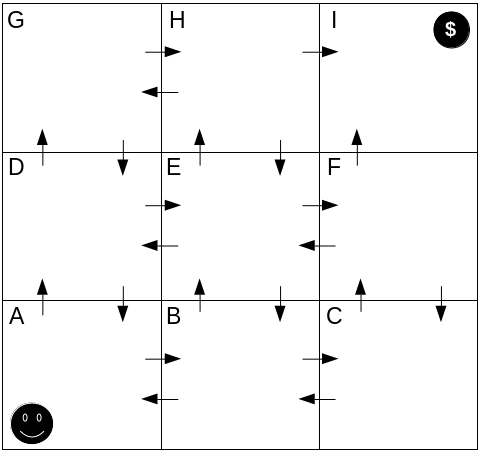
\includegraphics[width=0.45\textwidth]{img/exemplo-moeda-q-learning-1}
	\caption{Cenário da moeda na sua situação inicial}
	\label{fig:exemplo-moeda-q-learning}
\end{figure}

Para implementar o algoritmo de aprendizado por reforço para este agente, devemos definir o esquema de recompensas que o agente recebe, a estratégia com a qual o agente seleciona uma ação e o fator de desconto.
\begin{itemize}
	\item \textbf{Recompensas:} ao chegar no estado onde encontra-se a moeda, o agente recebe uma recompensa de 100. Nos demais estados o agente não recebe recompensa (ou seja, recebe 0). Consideremos ainda $I$ como o estado final e um estado de absorção.
	\item \textbf{Seleção de ações:} estratégia $\epsilon$-gulosa com $\epsilon = 0.2$.
	\item \textbf{Fator de desconto:} consideremos $\gamma = 0.9$.
\end{itemize}
.
Inicialmente, todas as entradas da tabela $\widehat{Q}(s, a)$ são inicializadas com zero, conforme a situação apresentada na Figura~\ref{fig:exemplo-moeda-q-learning}, em que nenhuma seta (ação) possui valor atribuído. Neste caso, todas as ações possuem recompensa esperada de zero, o que faz com que o agente selecione qualquer ação em qualquer estado que se encontre. Suponha que o agente selecione aleatoriamente a ação $A \rightarrow B$. Isso faz com que o agente receba recompensa imediata $r = 0$. A entrada correspondente da tabela $\widehat{Q}$ é atualizada conforme:

$$
\widehat{Q}(s, a) \gets r + \gamma \max_{a'} \widehat{Q}(s', a')
$$

Neste caso, $r = 0$ (recompensa imediata). Dado o novo estado $s' = B$, o agente deve verificar a melhor ação possível a partir de $B$ e somar a sua recompensa esperada, aplicando o desconto $\gamma$. A partir do estado $B$, todas as ações possuem recompensa esperada igual a 0. Logo, a entrada $\widehat{Q}(A, A \rightarrow B)$ permanece com o valor 0. Isso se repete enquanto o agente se movimenta no ambiente sem receber uma recompensa. Por exemplo, o agente poderia fazer o caminho $A \rightarrow B \rightarrow E \rightarrow D \rightarrow E \rightarrow H$. Ao selecionar uma ação que leva ao estado $I$ (por exemplo, $H \rightarrow I$), o agente recebe uma recompensa imediata $r = 100$. A recompensa futura esperada é 0, pois $I$ é um estado de absorção. Logo, $\widehat{Q}(H, H \rightarrow I) = 100$. Com isso, o primeiro episódio termina e a Figura~\ref{fig:exemplo-moeda-q-learning-2} apresenta o ambiente com os valores de recompensa atualizados.

\begin{figure}[h]
	\centering
	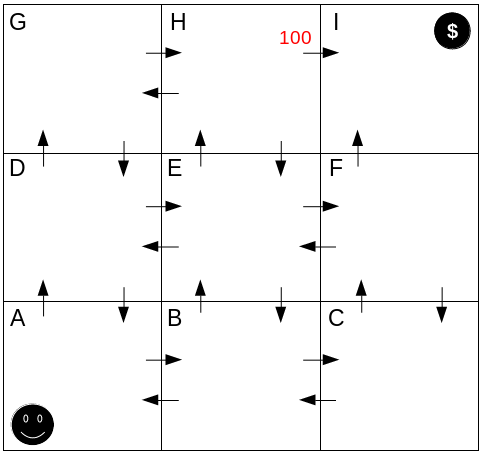
\includegraphics[width=0.44\textwidth]{img/exemplo-moeda-q-learning-2}
	\caption{Cenário da moeda ao encontrar o estado objetivo a partir de $H$}
	\label{fig:exemplo-moeda-q-learning-2}
\end{figure}

No segundo episódio, novamente o agente inicia no estado $A$ e não sabe qual a melhor ação a ser tomada, escolhendo aleatoriamente entre as ações disponíveis. Porém, suponhamos que o agente chegue no estado $G$ e selecione a ação $G \rightarrow H$. Neste caso, ele recebe uma recompensa imediata igual a 0, mas ao computar a recompensa futura, ele sabe que a partir de $H$ ele pode chegar a um estado com recompensa 100. Ou seja, $\max_{a'} \widehat{Q}(H, H \rightarrow I) = 100$. Logo, $\widehat{Q}(G, G \rightarrow H) = 0 + 0.9 \times 100 = 90$. Com isso, ao final do segundo episódio temos a situação apresentada na Figura~\ref{fig:exemplo-moeda-q-learning-3}.

\begin{figure}[h]
	\centering
	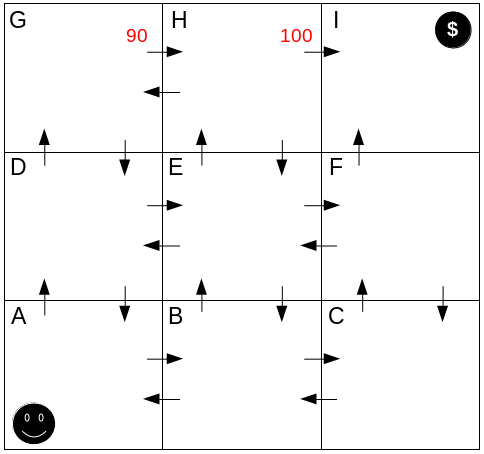
\includegraphics[width=0.44\textwidth]{img/exemplo-moeda-q-learning-3}
	\caption{Cenário da moeda ao encontrar um estado com recompensa futura}
	\label{fig:exemplo-moeda-q-learning-3}
\end{figure}

No terceiro episódio, novamente o agente inicia no estado $A$. Consideremos que o agente percorra o caminho $A \rightarrow B \rightarrow C \rightarrow F \rightarrow I$. Neste caso, ele só recebe uma recompensa quando atinge o estado $I$, fazendo com que a ação $F \rightarrow I$ receba o valor 100. Em um próximo episódio, uma ação que leve ao estado $F$ vai considerar a recompensa futura esperada da ação $F \rightarrow I$. Dessa forma, a cada episódio as recompensas são propagadas (aplicando o devido desconto), fazendo com que o conhecimento do agente sobre as melhores ações cresça. A Figura~\ref{fig:exemplo-moeda-q-learning-4} mostra uma situação intermediária, onde as recompensas já foram propagadas para vários pares $\langle s, a \rangle$. Perceba que, apesar do agente conhecer uma ação com uma grande recompensa $F \rightarrow I$, por exemplo, ele pode selecionar uma ação pior ou desconhecida para exploração, por exemplo $F \rightarrow E$. Este é o comportamento definido pela estratégia $\epsilon$-gulosa.

\begin{figure}[h]
	\centering
	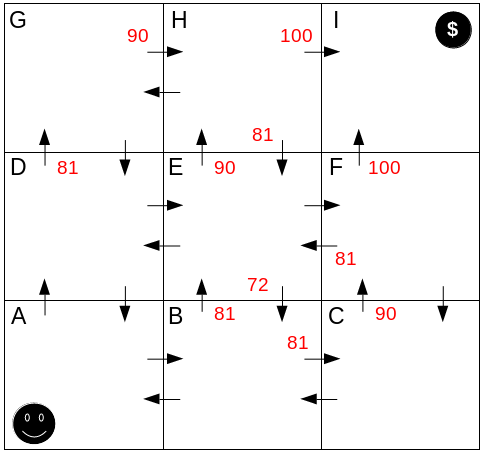
\includegraphics[width=0.44\textwidth]{img/exemplo-moeda-q-learning-4}
	\caption{Cenário da moeda com uma situação intermediária na execução do algoritmo}
	\label{fig:exemplo-moeda-q-learning-4}
\end{figure}

Ao final, desde que o número de episódios seja suficientemente grande, o algoritmo converge para a política ótima. Ou seja, a tabela $\widehat{Q}$ possui os valores de recompensa que fazem com que o agente siga a melhor sequência de ações possível. A Figura~\ref{fig:exemplo-moeda-q-learning-5} apresenta os valores de recompensa ao final da execução do algoritmo. Perceba que se o agente escolher a melhor ação de cada estado, ele chega ao destino com o menor número possível de passos. Perceba ainda que existem diferentes caminhos com o mesmo custo.

\begin{figure}[h]
	\centering
	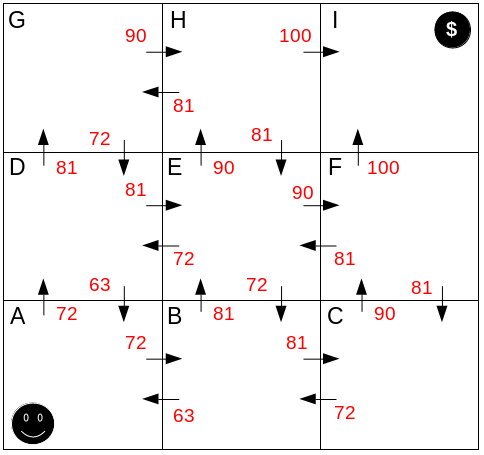
\includegraphics[width=0.44\textwidth]{img/exemplo-moeda-q-learning-5}
	\caption{Cenário da moeda ao finalizar a execução do algoritmo}
	\label{fig:exemplo-moeda-q-learning-5}
\end{figure}

Conforme discutido, a implementação de $\widehat{Q}$ geralmente é feita utilizando uma tabela com os estados $s \in S$ e as ações $a \in A$. A Tabela~\ref{tab:exemplo-moeda-q-learning} apresenta um exemplo de tabela $\widehat{Q}$ com os valores referentes ao estado intermediário apresentado na Figura~\ref{fig:exemplo-moeda-q-learning-4}. Para cada estado, o valor de recompensa esperada para cada ação é armazenado. Células com o caractere ``-'' indicam que não é possível realizar a respectiva ação no estado correspondente.

\begin{table}[h]
	\centering
	\begin{tabular}{r|ccccccccc}
		\multicolumn{1}{l|}{} & \textbf{A} & \textbf{B} & \textbf{C} & \textbf{D} & \textbf{E} & \textbf{F} & \textbf{G} & \textbf{H} & \textbf{I} \\ \hline
		\textbf{cima}         & 0          & 81         & 90         & 81         & 90         & 100        & -          & -          & -          \\
		\textbf{baixo}        & -          & -          & -          & 0          & 72         & 0          & 0          & 81         & -          \\
		\textbf{esquerda}     & -          & 0          & 0          & -          & 0          & 81         & -          & 0          & -          \\
		\textbf{direita}      & 0          & 81         & -          & 0          & 0          & -          & 90         & 100        & -         
	\end{tabular}
	\caption{Exemplo de tabela $\widehat{Q}$, representando a situação da Figura~\ref{fig:exemplo-moeda-q-learning-4}}
	\label{tab:exemplo-moeda-q-learning}
\end{table}

\clearpage

\section{Exercícios}

\resetexercisenumbering

\begin{exercise}
Mostre outras políticas ótimas para o ambiente em grade apresentado na Figura~\ref{fig:exemplo-rl-politica-otima}.
\end{exercise}

\begin{exercise}
Considere o cenário em grade apresentado abaixo com o estado objetivo de absorção \texttt{G}. A recompensa imediata é 10 para as transições rotuladas, e 0 para todas as demais.
\begin{enumerate}[a.]
	\item Apresente o valor de $V^*$ para cada estado do cenário. Apresente o valor de $Q(s, a)$ para cada transição. Finalmente, apresente uma política ótima. Use $\gamma = 0.8$.
	
	\item Sugira uma alteração na função de recompensa $r(s, a)$ que altera os valores de $Q(s, a)$, mas não altera a política ótima. Sugira uma mudança em $r(s, a)$ que altere $Q(s, a)$, mas não altere $V^*(s, a)$.
	
	\item Considere aplicar o algoritmo de $Q$-Learning no cenário em grade, assumindo que a tabela $\widehat{Q}$ é inicializada com zero. Assuma que o agente inicie na célula inferior esquerda e viaje no sentido horário ao redor do perímetro da grade, até encontrar o estado objetivo, completando o primeiro episódio. Descreva quais valores de $\widehat{Q}$ são modificados como resultado do episódio, e apresente seus valores atualizados. Responda à questão novamente, assumindo que o agente realize um episódio idêntico. Responda novamente para um terceiro episódio.
\end{enumerate}

\begin{figure}[h]
	\centering
	\includegraphics[width=0.25\textwidth]{img/exercicios/grade-rl}
\end{figure}
\end{exercise}

\begin{exercise}
O problema do penhasco é definido da seguinte forma:
\begin{itemize}
	\item Um robô está em uma sala mapeada como uma grade, conforme figura abaixo, onde seu objetivo é encontrar a saída. A posição inicial do robô é apresentada em verde, enquanto a porta é representada em azul. As células em vermelho compõem o penhasco. Logo, o robô deve aprender o menor caminho até a porta, sem que caia no penhasco.
	
	\item Os movimentos possíveis são \textit{cima}, \textit{baixo}, \textit{esquerda} e \textit{direita} (\textit{c}, \textit{b}, \textit{e}, \textit{d}).
	
	\item Ações que levariam o agente para fora da grade o deixam no mesmo lugar.
	
	\item Qualquer transição produz retorno imediato de -1, com exceção das que levam a estados do penhasco, que têm valor -100 e levam o agente de volta ao estado inicial.
\end{itemize}

\begin{figure}
	\centering
	\includegraphics[width=0.5\textwidth]{img/exercicios/problema-penhasco}
\end{figure}

Com base nisso, implemente o algoritmo de $Q$-Learning para fazer com que o agente aprenda a sair da sala. Implemente uma interface para que o usuário possa informar os parâmetros do algoritmo, conforme abaixo:
\begin{itemize}
	\item Número de episódios.
	\item Estratégia de seleção da ação: \textit{guloso} ou \textit{$\epsilon$-guloso}.
	\item Valor de $\epsilon$.
\end{itemize}

Apresente os resultados, mostrando:
\begin{itemize}
	\item A tabela $\widehat{Q}$ resultante.
	\item A política ótima.
	\item Quantos episódios o algoritmo levou até a convergência.
	\item Qual o resultado de cada episódio.
	\item Comparação entre as diferentes estratégias de seleção da ação e os diferentes valores de $\epsilon$.
\end{itemize}

\end{exercise}


\part{Apêndices}
\appendix
\chapter{Resoluções dos exercícios}
\renewcommand\thechapter{}
\renewcommand\thesection{\arabic{section}}

Este capítulo apresenta um direcionamento para a resolução dos exercícios. O pensamento, resolução ou descrição esperados são apresentados de forma resumida. É recomendável ao aluno apresentar respostas com o maior detalhamento possível, para praticar o entendimento completo de cada questão. Este aspecto é especialmente importante para as questões discursivas e aquelas solicitadas como parte de trabalhos e pesquisas da disciplina.

\section{Definição, histórico e paradigmas}

\begin{solution}
Definições:
\begin{enumerate}[a.]
	\item \textbf{Inteligência.} Algumas das definições encontradas no dicionário para inteligência são ``\textit{A capacidade de adquirir e aplicar conhecimento}'', ``\textit{A capacidade de pensamento e razão}'' e ``\textit{A capacidade de compreender e lucrar com a experiência}''. Todas essas são respostas razoáveis, mas se quisermos algo quantificável, usaríamos algo como ``\textit{A capacidade de aplicar conhecimento para melhorar o desempenho em um ambiente}''.
	
	\item \textbf{Inteligência artificial.} A inteligência artificial é definida como o estudo e construção de agentes inteligentes que façam um bom desempenho em um determinado ambiente, para uma determinada arquitetura de agente.
	
	\item \textbf{Racionalidade.} A racionalidade é definida como propriedade de um sistema que faz a ``coisa certa'' dado o que ele sabe.
\end{enumerate}
\end{solution}

\begin{solution}
Não. Os resultados dos testes de QI se correlacionam bem com certas outras medidas, como o sucesso na faculdade, capacidade de tomar boas decisões em situações complexas ou a capacidade de aprender novas habilidades e assuntos rapidamente. Porém, isso é válido apenas se os testes são aplicados a seres humanos. O teste de QI não mede tudo. Um programa que é especializado apenas para testes de QI (e se especializou apenas para a parte de analogia) provavelmente funcionaria mal em outras medidas de inteligência.

Considere a seguinte analogia: Se um humano executar os 100\,m em 10 segundos, podemos descrevê-lo como muito atlético e esperar desempenho competente em outras áreas, como caminhar, saltar, corrida com obstáculos, e talvez jogar bolas. Mas não descreveríamos um Boeing 747 como muito atlético porque pode percorrer 100\,m em 0,4 segundos, nem esperamos que ele seja bom em corrida com obstáculos e jogar bolas.
\end{solution}

\begin{solution}
\textbf{Leitores de código de barra de supermercados.} Embora a varredura de código de barras seja, em certo sentido, uma visão por computador, estes não são sistemas de IA. O problema de ler um código de barras é uma forma extremamente limitada e artificial de interpretação visual, e foi cuidadosamente projetada para ser o mais simples possível, dada a limitação de hardware.

\textbf{Menus de voz de telefones.} Em certa medida. Por exemplo, tais menus tendem a usar vocabulários e recursos muito limitados, como os dígitos ``Sim'' e ``Não''. Além disso, eles se limitam ao controle projetado, o que simplifica o problema. Por outro lado, os programas devem lidar com um espaço não controlado de todos os tipos de vozes e sotaques. Além disso, eles devem interpretar diferentes vocabulários, o que certamente os classifica como sistemas inteligentes.
	
\textbf{Mecanismos de busca na Web.} Determinar a relevância de uma página Web em uma consulta é um problema de processamento de linguagem natural. Os mecanismos de busca como o ``Ask.com'', que agrupam as páginas recuperadas em categorias, usam técnicas de agrupamento e aprendizagem de máquina. Do mesmo modo, outras funcionalidades fornecidas pelos motores de busca usam técnicas inteligentes. Por exemplo, o corretor ortográfico usa uma forma de mineração de dados com base na observação das correções dos usuários de seus próprios erros ortográficos. Por outro lado, o problema de indexar bilhões de páginas da Web de forma a permitir a recuperação em segundos é um problema no projeto do banco de dados, e não na inteligência artificial.
	
\textbf{Algoritmos de roteamento da Internet que respondem dinamicamente ao estado da rede.} Há algo a ser dito para vê-los como agentes inteligentes que trabalham no ciberespaço. A tarefa é sofisticada, a informação disponível é parcial, as técnicas são heurísticas (não garantidamente otimizadas) e o estado do mundo é dinâmico. Tudo isso é característico de atividades inteligentes. Por outro lado, a tarefa está muito longe daquelas normalmente realizadas na cognição humana.
\end{solution}

\begin{solution}
O prêmio Loebner 2017 está nas fases finais, mas sem vencedores até o momento. A edição de 2016 foi vencida por Mitsuku (programa) e Steve Worswick (autor). O diálogo entre os juízes e o robô pode ser visto em \url{http://www.aisb.org.uk/media/files/LoebnerPrize2016/Mitsuku.pdf}. Pelo diálogo, pode-se perceber que o processamento de linguagem natural é fundamental para estabelecer uma comunicação inteligente entre os juízes e a máquina. Além disso, as perguntas exigem habilidades como a aprendizagem de máquina, representação do conhecimento, raciocínio, etc. É possível conversar com este robô em \url{http://www.mitsuku.com/}. Mais detalhes sobre as edições do prêmio Loebner podem ser consultados em \url{http://www.aisb.org.uk/events/loebner-prize}.
\end{solution}

\begin{solution}
Observações:
\begin{enumerate} [a.]
	\item  \textbf{Tênis de mesa.} Um nível razoável de proficiência foi alcançado pelo robô de~\citet{Andersson1988}.
	
	\item \textbf{Dirigir no centro de Cairo.} Sim. Apesar dos desafios que os pesquisadores de veículos autônomos ainda precisam superar, todas as grandes dificuldades já foram vencidas e a tarefa de condução autônoma já é uma realidade. Em países como Estados Unidos e Alemanha os investimentos resultaram em vários veículos autônomos circulando pelas cidades.
	
	\item \textbf{Compras no mercado.} Não. Nenhum robô pode atualmente juntar as tarefas necessárias para esta atividade, como se deslocar em um ambiente lotado, usar a visão computacional para identificar uma grande variedade de objetos, coletar os objetos desejados sem danificá-los, etc. As tarefas individuais são possíveis, mas seria necessário um grande esforço de integração para juntar tudo.
	
	\item \textbf{Compras na Internet.} Sim. Robôs de software são capazes de lidar com tais tarefas, especialmente se a estrutura do site de compras na Web não muda radicalmente ao longo do tempo.
	
	\item \textbf{Jogar \textit{bridge}.} Sim. Programas como o GIB (veja detalhes em \url{http://www.gibware.com/}) jogam em um nível sólido.
	
	\item \textbf{Prova de teoremas.} Sim. Por exemplo, o cálculo da álgebra de Robbins.
	
	\item \textbf{Escrever uma história engraçada.} Não. Enquanto algumas prosas e poesias geradas por computadores são histericamente engraçadas, isso é invariavelmente não intencional, exceto no caso de programas que retornam a prosa que memorizaram.
	
	\item \textbf{Assessoria jurídica.} Sim, em alguns casos. A inteligência artificial tem uma longa história de pesquisa em aplicações de raciocínio jurídico automatizado. Dois exemplos notáveis são os sistemas especialistas baseados em Prolog utilizados no Reino Unido para orientar os membros do ministério público a lidar com as leis de seguridade social e nacionalidade. É previsto que o sistema de seguridade social do governo do Reino Unido tenha economizado aproximadamente U\$ 150 milhões em seu primeiro ano de operação. Contudo, a extensão a áreas mais complexas, como o direito dos contratos, prevê uma codificação satisfatória da vasta rede de conhecimentos de bom senso relativos a transações, práticas e acordos comerciais.
	
	\item \textbf{Tradução de idiomas.} Sim. De forma limitada, isso já está sendo feito e tem evoluído com o passar do tempo, sobretudo pelas técnicas de aprendizagem de máquina que melhoram o desempenho das traduções com base nos dados de experiências passadas.
	
	\item \textbf{Operação cirúrgica.} Sim. Os robôs são cada vez mais usados para a cirurgia, embora sempre sob o comando de um médico. As habilidades robóticas demonstradas em níveis sobre-humanos incluem perfuração de buracos no osso para inserir juntas artificiais, sutura e nó de amarração. Eles ainda não são capazes de planejar e executar uma operação complexa de forma autônoma do início ao fim.
\end{enumerate}
\end{solution}

\clearpage

\section{Agentes inteligentes}
\resetsolutionnumbering

\begin{solution}
Ambientes de tarefa:
\begin{table}[h]
	\centering
	\small
	\rowcolors{2}{white}{gray!25}
	\begin{tabular}{L{2cm} L{3cm} L{3cm} L{2.9cm} L{2.9cm}}
		\hline
		\rowcolor{black}
		\color{white}\textbf{Agente} & \color{white}\textbf{Medida de desempenho} & \color{white}\textbf{Ambiente} & \color{white}\textbf{Atuadores} & \color{white}\textbf{Sensores} \\
		\hline
		Jogar futebol & Número de gols, tempo de posse de bola, número de faltas & Campo, traves, áreas, bola, outros jogadores & Pernas e braços robóticos & Câmera, sonar \\
		Compra de livros na Internet & Preço, qualidade do livro, prazo de entrega & Sites de vendas, grupos de venda em redes sociais & Cartão de crédito & Algoritmo de leitura de conteúdo da Web \\
		Jogar uma partida de tênis & Pontuação, tempo de partida & Quadra, rede, raquete, bola, adversário & Pernas e braços robóticos & Câmera, sonar \\
		Praticar tênis na parede & Tempo sem deixar a bola cair & Limites no solo, parede, raquete, bola & Pernas e braços robóticos & Câmera \\
		Realizar um salto em altura & Altura do salto & Obstáculo, pista & Pernas robóticas & Câmera \\
		Licitações de um item em um leilão & Compra do item, valor pago & Site do leilão, ofertas, compradores & Função de lance & Leitor do site do leilão \\
		\hline
	\end{tabular}
\end{table}
\end{solution}

\begin{solution}
Classificação dos ambientes:
\begin{enumerate}[a.]
	\item \textbf{Jogo de palavras cruzadas:} completamente observável, determinístico, sequencial, estático, discreto e monoagente.
	\item \textbf{Xadrez com relógio:} completamente observável, determinístico, sequencial, semi-dinâmico, discreto e multiagente.
	\item \textbf{Pôquer:} parcialmente observável, estocástico, sequencial, estático, discreto e multiagente.
	\item \textbf{Gamão:} completamente observável, estocástico, sequencial, estático, discreto e multiagente.
	\item \textbf{Veículo autônomo:} parcialmente observável, estocástico, sequencial, dinâmico, contínuo e multiagente.
	\item \textbf{Diagnóstico médico:} parcialmente observável, estocástico, sequencial, dinâmico, contínuo e monoagente.
	\item \textbf{Análise de imagens:} completamente observável, determinístico, episódico, semi-dinâmico, contínuo e monoagente.
	\item \textbf{Robô de seleção de peças:} parcialmente observável, estocástico, episódico, dinâmico, contínuo e monoagente.
	\item \textbf{Controlador de refinaria:} parcialmente observável, estocástico, sequencial, dinâmico, contínuo e monoagente.
	\item \textbf{Instrutor interativo de inglês:} parcialmente observável, estocástico, sequencial, dinâmico, discreto e multiagente.
\end{enumerate}
\end{solution}

\begin{solution}
Exercício de implementação.
\end{solution}

\begin{solution}
Exercício de implementação.
\end{solution}

\begin{solution}
Aspirador de pó com penalidade:
\begin{enumerate}[a.]
	\item Não. Se o agente possui percepção apenas do quadrado onde se encontra, ele não pode decidir sobre não mais se movimentar. Somente com a observação completa do cenário o agente reativo consegue verificar que todos os quadrados já estão limpos e, com isso, não mais se movimentar. Para ser racional com observação parcial, o agente deve manter em memória as percepções anteriores, deixando de ser um agente reativo simples.
	
	\item Sim. Conforme discutido no item anterior, se o agente pode manter em memória os demais quadrados do ambiente, ele passa a ser racional.
	\begin{itemize}
		\item \textbf{Medida de desempenho:} agente recebe 100 pontos para cada quadrado limpo ao fim do dia e -1 ponto para cada movimento.
		\item \textbf{Conhecimento do agente sobre o ambiente:} o agente conhece a geografia do ambiente e desconhece a distribuição da sujeira e sua posição inicial. Quadrados limpos permanecem limpos até o fim do dia. A ação de aspiração limpa o quadrado onde o agente se encontra. As ações \textit{esquerda} e \textit{direita} movem o agente para os quadrados adjacentes (conforme o lado escolhido). O agente não pode se movimentar para fora do ambiente. O agente mantém uma memória interna (modelo) com as percepções e ações anteriores.
		\item \textbf{Ações:} \textit{esquerda}, \textit{direita}, \textit{aspirar} e \textit{nada}.
		\item \textbf{Percepções:} agente percebe sua posição e se a posição contém sujeira.
		\item \textbf{Observações:} para a racionalidade, os fatos dos quadrados permanecerem limpos e da ação \textit{aspirar} ser perfeita são fundamentais.
	\end{itemize}
	
	\item Neste caso, um agente reativo simples pode ser perfeitamente racional. Cada percepção mostra o estado (limpo/sujo) de cada quadrado. Com isso, o agente pode agir, limpando um quadrado, por exemplo. A percepção seguinte apontará para o estado completo atualizado, tornando o agente racional.
\end{enumerate}
\end{solution}

\begin{solution}
Aspirador de pó aleatório:
\begin{enumerate}[a.]
	\item Não. Se o agente não conhece a geografia do ambiente, percebe apenas a sua localização e a sujeira deste local e ainda não armazena em memória o que acabou de fazer, ele não tem como tomar a decisão que maximiza sua função de desempenho. Por exemplo, ele ficará preso para sempre contra um parede quando tentar se mover e a direção estiver bloqueada. Para superar esta dificuldade, o agente deveria aplicar alguma aleatoriedade, mas isso não leva à racionalidade.
	
	\item Uma possibilidade é um agente que limpa a sujeira do quadrado onde se encontra e se move aleatoriamente. Esta abordagem supera um agente reativo simples, pois este último pode ficar preso infinitamente em uma ação, conforme discutido no item anterior. Logo, a aleatoriedade ajudaria a superar estas dificuldades. Isso é muito parecido com o que um aspirador \textit{Roomba} faz (apesar de que o \textit{Roomba} usa um sensor de toque e age aleatoriamente somente quando acerta um obstáculo). Ele funciona razoavelmente bem em ambientes compactos. Em ambientes que se assemelham a labirintos ou aqueles com passagens estreitas ele pode demorar bastante para cobrir todos os quadrados.
	\begin{itemize}
		\item Exercício de implementação.
	\end{itemize}
	
	\item O ambiente da figura abaixo apresenta dificuldade para um agente com aleatoriedade de movimento. A aleatoriedade dificulta superar os corredores para acesse de um quadrado a outro.
	
	\begin{figure}[h]
		\centering
		\includegraphics[width=0.5\textwidth]{img/exercicios/ambiente-dificil-aleatoriedade}
	\end{figure}
	
	\item Um agente reativo com estado pode construir internamente uma representação (mapa) do ambiente. Uma busca em profundidade encontrará todos os estados em tempo linear de acordo com o tamanho do ambiente. Portanto o agente pode ter um desempenho muito superior a um agente reativo.
	\begin{itemize}
		\item Exercício de implementação.
	\end{itemize}
\end{enumerate}
\end{solution}

\clearpage

\section{Buscas em espaços de estados}

\resetsolutionnumbering

\begin{solution}
Definições:
\begin{itemize}
	\item Um \textbf{estado} é a situação em que um agente pode se encontrar. Distinguimos dois tipos de estados: \textit{estado do mundo} -- as situações concretas no mundo real e \textit{estados de representação} -- representações abstratas do mundo real que são usadas pelos agentes nas decisões do que fazer.
	
	\item Um \textbf{espaço de estado} é um grafo cujos formam o conjunto de todos os estados possíveis e os arcos são ações que transformam um estado em outro (ou que levam o agente de um estado a outro).
	
	\item A \textbf{árvore de busca} é uma árvore (um grafo direcionado acíclico) na qual o nó raiz é o estado inicial e o conjunto de filhos de cada nó consiste nos estados alcançáveis na tomada de qualquer ação.
	
	\item Um \textbf{nó de busca} é um nó na árvore de busca.
	
	\item Uma \textbf{ação} é alguma coisa que o agente pode escolher fazer.
	
	\item O \textbf{objetivo} consiste no estado que o agente está tentando alcançar.
	
	\item O \textbf{modelo de transição}, também chamado de \textbf{função sucessor}, é especificado por uma função $sucessor(a, s)$ que devolve o estado que resulta de executar uma ação $a$ em um estado $s$.
	
	\item O \textbf{fator de ramificação} em uma árvore de busca é o maior número de sucessores que um nó pode conter.
\end{itemize}
\end{solution}

\begin{solution}
Um \textbf{estado do mundo} consiste em como a realidade é ou poderia ser. O estado do mundo pode ser \textit{Arad} ou \textit{Bucharest}, por exemplo. O estado do mundo inclui todo e qualquer detalhe do mundo real, como a rua em que estamos, o que está tocando no rádio e o preço do chá na China. Uma \textbf{descrição do estado} é a definição interna que um agente possui de um estado do mundo. Por exemplo, o agente precisa saber somente sua localização (\textit{Arad} ou \textit{Bucharest}), e não todos os detalhes que não influenciam na execução da tarefa desejada. Ou seja, essas descrições são aproximadas, mantendo apenas alguns aspectos do estado do mundo.  Precisamos diferenciar \textbf{estados do mundo} de \textbf{descrição do estado}, pois descrições de estados são abstrações do estado do mundo e podem conter perdas.

Os \textbf{nós de busca} são gerados durante a busca, representando um estado em que o processo de busca sabe como chegar. Eles contêm informações adicionais além da descrição do estado, como a sequência de ações usadas para alcançar esse estado. Essa distinção é útil porque podemos gerar diferentes nós de busca que possuem o mesmo estado, além de apresentarem mais informações que uma representação do estado.
\end{solution}

\begin{solution}
Problema de roteamento entre dois amigos.
	\begin{enumerate}[a.]
		\item Formulação:
		\begin{itemize}
			\item \textbf{Espaço de estados:} todos os pares possíveis de cidades $(i, j)$. O mapa não é o espaço de estados.
			
			\item \textbf{Função sucessor:} os sucessores de $(i, j)$ são todos os pares $(x, y)$, tal que $x$ seja adjacente de $i$ e $y$ seja adjacente de $j$.
			
			\item \textbf{Objetivo:} estar em $(i, i)$ para qualquer cidade $i$.
			
			\item \textbf{Custo de passo:} o custo de ir de $(i, j)$ para $(x, y)$ é $max(d(i, x), d(j, y))$.
		\end{itemize}
	
		\item No melhor caso, os amigos se dirigem um em direção ao outro em passos de tamanho igual. Isso reduz a separação entre eles por duas vezes o custo de cada passo. Portanto, as heurísticas (i) e (ii) superestimam o custo até a solução. A heurística (iii) é a única admissível.
	
		\item Sim. Um exemplo consiste em um mapa com dois nós conectados por um link. Os dois amigos trocarão de lugares para sempre. O mesmo vai acontecer em qualquer sequência se eles começarem em um número ímpar de passos separados.
	
		\item Sim. Dado um mapa sem solução da questão (c), podemos adicionar um auto-loop (caminho de um estado para si mesmo) a qualquer um dos nós. Se os amigos começam em um número ímpar de passos separados, um movimento no qual um dos amigos toma o auto-loop altera a distância em 1, tornando o problema solucionável. Se o auto-loop não for tomado, o argumento de (c) se aplica e nenhuma solução é possível.
	\end{enumerate}
\end{solution}

\begin{solution}
Formulação de problemas:
\begin{enumerate}[a.]
	\item Coloração de mapa
	\begin{itemize}
		\item \textbf{Estado inicial:} sem região colorida.
		\item \textbf{Teste de objetivo:} todas as regiões coloridas sem que duas regiões adjacentes contenham a mesma cor.
		\item \textbf{Função sucessor:} atribuir uma cor para uma região.
		\item \textbf{Função de custo:} número de atribuições.
	\end{itemize}
	
	\item Macaco e as bananas:
	\begin{itemize}
		\item \textbf{Estado inicial:} como descrito no enunciado.
		\item \textbf{Teste de objetivo:} macaco apanha as bananas.
		\item \textbf{Função sucessor:} subir no engradado; descer do engradado; mover engradado de um ponto a outro; caminhar de um ponto a outro; apanhar as bananas (apenas se puder alcançá-las).
		\item \textbf{Função de custo:} número de ações.
	\end{itemize}	
	
	\item Problema dos jarros:
	\begin{itemize}
		\item \textbf{Estado inicial:} jarras com valores $[0, 0, 0]$.
		\item \textbf{Função sucessor:} dados os valores $[x, y, z]$, gera $[12, y, z]$, $[x, 8, z]$, $[x, y, 3]$ (ação de enher); $[0, y, z]$, $[x, 0, z]$, $[x, y, 0]$ (ação de esvaziar); ou para quaisquer duas jarras com valores atuais $x$ e $y$, despeje $y$ em $x$; Isso muda a jarra com $x$ para o mínimo de $x + y$ e a capacidade da jarra, e diminui a jarra com $y$ pelo valor obtido pela primeira jarra.
		\item \textbf{Função de custo:} número de ações.
	\end{itemize}
	
\end{enumerate}
\end{solution}

\begin{solution}
Custos negativos nos caminhos:
\begin{enumerate}[a.]
	\item Qualquer caminho, por pior que pareça, pode levar a uma recompensa arbitrariamente grande (custo negativo). Portanto, seria necessário explorar todos os caminhos possíveis para se ter certeza que encontraria o melhor.
	
	\item Suponha que a maior recompensa possível é $c$. Então, se conhecemos a profundidade máxima do espaço de estados, qualquer caminho com $d$ níveis restantes pode ser melhorado por no máximo de $c \times d$. Sendo $x$ o custo do melhor caminho e $y$ o custo de um candidato, sabemos que o candidato poderá ter custo não inferior a $y + c \times d$. Logo, se $y + c \times d > x$, o caminho candidato pode ser podado. Para espaços de estados com loops esta garantia não ajuda, pois é possível dar uma volta a um loop várias vezes, escolhendo a recompensa $c$ a cada vez. 
	
	\item O agente deve planejar dar uma volta a esse ciclo para sempre (a menos que possa encontrar outro loop com uma recompensa ainda melhor).
	
	\item O valor associado a uma bela paisagem é menor quando ela é revisitada. Uma paisagem nunca vista provoca uma grande recompensa, mas o mesmo não acontece quanto ela é revisitada muitas vezes. Neste caso, a paisagem passa a ser entediante, não provocando nenhuma recompensa. Para implementar isso, devemos expandir o espaço de estados incluindo um estado com memória. A representação de um estado não inclui apenas a localização, mas um conjunto de localizações já visitadas. A recompensa por visitar uma nova localização é agora implementada por uma função do número de vezes que ela foi visitada anteriormente.
\end{enumerate}
\end{solution}

\begin{solution}
Missionários e canibais:
\begin{enumerate}[a.]
	\item Aqui está uma representação possível: um estado é uma tupla de 6 números inteiros, que correspondem à quantidade de missionários, canibais e barcos em cada lado do rio. O objetivo é um estado com 3 missionários e 3 canibais no segundo lado do rio. A função de custo é 1 para cada ação executada. Os sucessores de um estado são todos os estados, que configuram a movimentação de uma ou duas pessoas e um barco para o outro lado do rio.
	
	\item Exercício de implementação. O espaço de busca é pequeno, então qualquer algoritmo ótimo funciona. Isso é suficiente para eliminar movimentos que voltam para um estado já visitado.
	
	\item Não é evidente que quase todos os movimentos são inválidos ou revertem para um estado anterior. Existe uma sensação de um grande fator de ramificação e nenhuma maneira clara de prosseguir.
\end{enumerate}

\begin{figure}[h]
	\centering
	\includegraphics[width=0.85\textwidth]{img/exercicios/missionarios-canibais}
\end{figure}
\end{solution}

\insertspace
\insertspace

\begin{solution}
O espaço de estados é uma árvore com profundidade igual a 1, com todos os estados sendo sucessores do estado inicial. Não há distinção entre uma busca em largura e uma busca em profundidade nesta árvore. Se o comprimento da sequência for ilimitado, o nó da raiz terá infinitos sucessores, então um simples algoritmo de teste dos nós sucessores pode funcionar.

O que acontece depois depende de como as ações compostas são classificadas. Se não existe uma ordenação específica, então ocorre uma busca aleatória (porém sistemática) de possíveis soluções. Se eles são ordenados por ordem alfabética, é implementada uma busca em largura.

Uma importante desvantagem de suprimir o espaço de busca dessa forma, ocorre se descobrimos que um plano que inicia com a ação $x$ não compõe a solução. Neste caso, não existe uma maneira simpes de ignorar todas as outras ações compostas que iniciam com a ação $x$. Isto é um problema em particular para algoritmos de busca informados.

Descartar a estrutura de sequência não é uma abordagem particularmente prática para a pesquisa.
\end{solution}

\begin{solution}
Observações:
\begin{enumerate}[a.]
	\item \textbf{Falso.} Uma busca em profundidade com sorte pode expandir exatamente $d$ nós para atingir o objetivo. A busca A* domina com folga qualquer algoritmo de busca que garanta a otimalidade.
	
	\item \textbf{Verdadeiro.} $h(n) = 0$ é sempre uma heurística admissível, uma vez que os custos são não-negativos.
	
	\item \textbf{Verdadeiro.} A busca A* é utilizada na robótica. O espaço pode ser discretizado. 
	
	\item \textbf{Verdadeiro.} Para a busca em largura, o que influencia é a profundidade da solução, não o custo. O custo influencia apenas na otimalidade da busca.
	
	\item \textbf{Falso.} Uma torre pode se mover ao longo de todo o tabuleiro em apenas um movimento. No entanto, a distância de Manhattan calcula um custo de 8 para um movimento ao longo do tabuleiro.
\end{enumerate}
\end{solution}

\begin{solution}
Problema $2k$ / $2k + 1$:
\tikzset{
	treenode/.style = {align=center, inner sep=0pt, text centered,font=\sffamily},
	no/.style = {treenode, circle, black, font=\sffamily\bfseries, draw=black,fill=white, text width=1.5em}
}

\begin{enumerate}[a.]
	\item Representação:
	
	\begin{figure}[h]
		\centering
		\begin{tikzpicture}[->,>=stealth',level/.style={sibling distance = 5cm/#1,level distance = 1.5cm}] 
			\node [no] {1}
			child{ node [no] {2} 
				child{ node [no] {4} 
					child{ node [no] {8}}
					child{ node [no] {9}}
				}
				child{ node [no] {5}
					child{ node [no] {10}}
					child{ node [no] {11}}
				}                            
			}
			child{ node [no] {3}
				child{ node [no] {6} 
					child{ node [no] {12}}
					child{ node [no] {13}}
				}
				child{ node [no] {7}
					child{ node [no] {14}}
					child{ node [no] {15}}
				}
			}
			; 
		\end{tikzpicture}
	\end{figure}
	
	\item Ordem de visitação
	\begin{itemize}
		\item \textbf{Busca em largura:} 1 2 3 4 5 6 7 8 9 10 11.
		\item \textbf{Busca em profundidade limitada:} 1 2 4 8 9 5 10 11.
		\item \textbf{Busca em profundidade iterativa:} 1; 1 2 3; 1 2 4 15 3 6 7; 1 2 4 8 9 5 10 11.
	\end{itemize}
	
	\item A busca bidirecional torna-se útil ao problema, já que o único sucessor de $n$ na direção inversa é $\lfloor(n / 2)\rfloor$. Isso ajuda a focar a busca. O fator de ramificação é 2 na direção normal e 1 na direção inversa.
	
	\item Sim. Comece no objetivo e aplique a única ação de sucessor reverso até chegar a 1.
	
	\item A solução pode ser lida com o número binário do valor objetivo. Como só podemos alcançar números inteiros positivos, essa expansão binária inicia com o valor 1. Do bit mais significativo ao menos significativo, pulando o 1 inicial, vá para a esqueda no nó $2n$ se esse bit for 0 e vá para a direita no nó $2n + 1$, caso seja 1. Por exemplo, suponha que o objetivo seja 11, que em binário é 1011. A solução é, portanto: esquerda, direita, direita.
\end{enumerate}

\end{solution}

\begin{solution}
A sequência de filas é a seguinte:

\begin{itemize}[itemsep=10pt]
	\item L[0+244=244]
	\item M[70+241=311], T[111+329=440]
	\item L[140+244=384], D[145+242=387], T[111+329=440]
	\item D[145+242=387], T[111+329=440], M[210+241=451], T[251+329=580]
	\item C[265+160=425], T[111+329=440], M[210+241=451], M[220+241=461], T[251+329=580]
	\item T[111+329=440], M[210+241=451], M[220+241=461], P[403+100=503], T[251+329=580], R[411+193=604], D[385+242=627]
	\item M[210+241=451], M[220+241=461], L[222+244=466], P[403+100=503], T[251+329=580], A[229+366=595], R[411+193=604], D[385+242=627]
	\item M[220+241=461], L[222+244=466], P[403+100=503], L[280+244=524], D[285+242=527], T[251+329=580], A[229+366=595], R[411+193=604], D[385+242=627]
	\item L[222+244=466], P[403+100=503], L[280+244=524], D[285+242=527], L[290+244=534], D[295+242=537], T[251+329=580], A[229+366=595], R[411+193=604], D[385+242=627]
	\item P[403+100=503], L[280+244=524], D[285+242=527], M[292+241=533], L[290+244=534], D[295+242=537], T[251+329=580], A[229+366=595], R[411+193=604], D[385+242=627], T[333+329=662]
	\item B[504+0=504], L[280+244=524], D[285+242=527], M[292+241=533], L[290+244=534], D[295+242=537], T[251+329=580], A[229+366=595], R[411+193=604], D[385+242=627], T[333+329=662], R[500+193=693], C[541+160=701]
\end{itemize}
\end{solution}

\begin{solution}
Exercício de implementação.
\end{solution}

\begin{solution}
Exercício de implementação.	
\end{solution}

\begin{solution}
Exercício de implementação.
\end{solution}

%\clearpage

%\section{Metaheurísticas}

%\section{Conceitos básicos de aprendizagem de máquina}

%\section{Aprendizado supervisionado}

%\section{Aprendizado não supervisionado}

%\section{Aprendizado por reforço}

\addcontentsline{toc}{chapter}{Referências Bibliográficas}
\nocite{*}
\bibliographystyle{apalike}
\bibliography{referencias}

\end{document}